

\documentclass{trkut}
\usepackage[style=trkut]{biblatex}
\addbibresource{viited_EesnimiPerekonnanimi.bib}
\setmainfont{Times New Roman} 
%\usepackage{tgtermes}

%\theoremstyle{plain}


\usepackage{pdfpages, newfloat, amsmath, amsthm, float, minted}

%\theorembodyfont{\normalfont}

\theoremstyle{definition}

\DeclareFloatingEnvironment[fileext=lop, name=Koodilõik,within=none]{kk}

\usepackage[many]{tcolorbox}
\tcbuselibrary{minted}

\newtcblisting{cclol}{
  colframe=cyan,
  colback=cyan!10,
  listing only,
  breakable,
  listing engine=minted,
  minted language=cpp,
  minted options={fontsize=\normalsize,linenos,numbersep=6mm},
}

% Kuidas teha peatükk ilma numbrita

\newtheorem*{prereq}{Eelteadmised}
\newtheorem*{extra}{NB}
\newtheorem*{vihje}{Vihje}
\newtheorem*{solution}{Täislahendus}
\newtheorem*{Input}{Sisend}
\newtheorem*{Output}{Väljund}
\newtheorem*{Text}{Ülesanne}
\newtheorem*{subtasks}{Alamülesanded}

\usepackage{hyperref}

\pealkiri{Lõikude puu andmestruktuur võistlusprogrammeerimises}
\autor{Karl Erich Kaugeranna}
\klass{139. a, reaal-programmeerimise  õppesuund}
\juhendaja{Jaagup Kippar}

\begin{document}
\maketitle%
\tableofcontents%
\addchap{Sissejuhatus}

Uurimistöös käsitletakse lõikude puud ning selle abil lahendatavaid ülesandeid võistlusprogrammeerimises. Uurimistöö aktuaalsus tuleneb sellest, et lõikude puu on väheuuritud, kuid teoreetiliselt kasulik andmestruktuur, ning varasemad materjalid ei ole kokkuvõtlikud, orienteeritud võistlusprogrammeerimisele, ega eesti keeles.

Uurimistöö uurimisküsimusteks on, et millal on mõistlik lahendada ülesannet lõikude puu abil ja kuidas lahendada ülesandeid lõikude puuga seotud võtete abil.

Uurimistöö teoreetilises osas antakse ülevaade lõikude puu teoreetilistest omadustest ja selle implementatsioonist programmeerimiskeeles C++.

Uurimistöö praktilises osas lahendatakse läbi mitmeid lõikude puuga seotud ülesandeid erinevatest allikatest, kirjeldades nende lahendusi, selgitatakse välja millal on mõistlik või võimalik kasutada lõikude puud ülesande lahendamisel, koostatakse samaaegselt ülesannete kogum, mis on järjekorras milles on neid mõistlik lahendada. Koostatakse ka kaks lõikude puuga lahendatavat ülesannet järgides informaatikaolümpiaadile omaste ülesannete struktuuri.

Uurimistöö teoreetilises osas kasutatud põhiallikateks on veebis kättesaadav avatud lähtekoodiga õppematerjal Algorithms for Competitive Programming, vabavara initsiatiiv USACO Guide, Antti Laaksoneni e-raamat Competitive Programmer’s Handbook ning Targo Tennisbergi ja Katrin Gabreli eestikeelne võistlusprogrammeerimise e-raamat.

Uurimistöö autor soovib tänada oma juhendajat õpetaja Jaagup Kipparit aktiivse ja põhjaliku tagasiside eest. 
Autor tänab ka Tartu Ülikooli lõpetanud MSc Tähvend Uustalut, kes vaatas töö üle, ning tegi selgeks veakohad, Eesti Informaatikaolümpiaadi žürii esimeest Sandra Schumanni abivalmiduse ja kontaktide loomise eest, ning Gustav Adolfi Gümnaasiumi õpilast Marten Mehidet ülesande Kaardid lahenduse selgitamise eest.

\chapter{Lõikude puu andmestruktuur, erinevaid võtteid}
Enne siit jätkamist peaks olema lugeja kindlasti tuttav vähemalt graafiteooria põhimõistetega, need on välja toodud ka lisades(vt Lisa 1, 2).

Lõikude puu on tasakaalustatud kahendpuu kujuline andmestruktuur, mis hoiab andmeid massiivi lõikude kohta.

Suure-O notatsiooni halvima juhu mõiste põhjal on lõikude puu ruumi keerukus $O(N)$ ja konstrueerimise(hiljem konstrueerimine või ehitamine) ajaline keerukus samuti $O(N)$. \parencite{ITS}

Levinumate operatsioonide RMQ(miinimumi leidmine lõigus) ja lõigu summa leidmise ajaliseks keerukuseks on $O(\log N)$.
Samuti võimaldab lõikude puu pärast konstrueerimist tippude väärtuste muutmist. \parencite{EMaxx}

\section{Lõikude puu struktuur}
Lõikude puu struktuuri selgitamisel lähtun alustuseks lihtsaimast operatsioonist -- lõikude summade leidmine.

Omades massiivi $a[0...N-1]$ peab lõikude puu olema võimeline arvutama elementide summa indeksite $l$ ja $r$ vahel s.t leidma $\sum_{i=l}^{r} {a[i]}$ ja samuti võimaldama tehteid kujul $a[i] = x$, kus x on vabalt valitud väärtusega andmetüübi piirides. Mõlemad operatsioonid on tehtavad ajakeerukusega $O(\log N)$. \parencite{EMaxx}

Arvutame lõikude väärtused jaga-ja-valitse algoritmidele kohaselt ehk leiame ja salvestame $a[0...N-1]$ summa, seejärel $a[0...N/2-1]$ ja $a[N/2...N-1]$ jne kuni puu lehtedeni välja mille summad on võrdsed üheainsa elemendi väärtusega. \parencite{EMaxx}

\begin{figure}[H]% [] sisse märgitakse paigutus H
    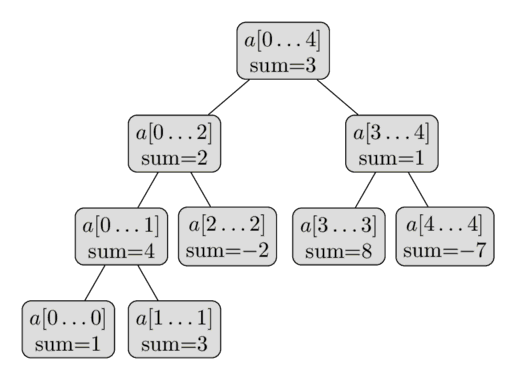
\includegraphics[width=8cm]{LPUU.png}% Joonise suurus, joonise fail
    \caption{Massiivil $a[1,3,-2,8,-7]$ põhineva lõikude puu struktuur}% Allkiri
    \allikas{Algorithms for Competitive Programming}% Allikas
    \label{CPH}% Selle järgi viidatakse, pärast käsku \caption
\end{figure}

Sellepärast et alates juurest paardub iga tipp kaheks tipuks(mis on kahendpuu tunnuseks), saame järeldada et $N$ suurusega massiivil üles ehitatud lõikude puu vajab maksimaalselt $4N$ tippu(juhul kui alustada indekseerimist 0-ist piisab ka $2N$ suurusega massiivist). \parencite{EMaxx}

Implementeerides on kasulik täheldada et kui $N$ ei ole kahe aste, ei ole tegu perfektse kahendpuuga, vaid ainult tasakaalustatud kahendpuuga. 

Lõikude puus juurtipu kõrguseks on $\Theta(\log N)$, ümardades üles. \parencite{EMaxx}

See on formaalselt selgitatav, kui teada mõnda asjaolu:

Tähistagu $h$ puu kõrgust ja $l_i$ tasemel $i$ olevate tippude arvu.
\begin{enumerate}
    \item $l_1 = 1$, ehk esimesel tasemel on üks tipp(juur).
    \item $l_k = 2l_{k−1}$, ehk igal tasemel on kaks korda rohkem tippe kui eelmisel tasemel.
    \item Eelmised võrrandid on teisendatavad kujule $l_k = 2^{k−1}$.
\end{enumerate}

Veel teame, et tippude arv $N$, on võrdne iga taseme tippude summaga:

$1 + 2^1 + 2^2 + 2^3 + ... + 2^{h−1} = N$

Teama ka, et:

$1 + 2^1 + 2^2 + 2^3 + ... + 2^{h−1} = 2^h − 1$

Järelikult:
    
$2^h − 1 = N$

$2^h = N + 1$
 
$\log_2 2^h = \log_2 (N + 1)$

$h \log_2 2 = \log_2 (N + 1)$

$h = \log_2(N + 1)$

Saamegi et puu kõrgus on $\Theta(\log N)$. \parencite{height}

\section{Lõikude puu ehitamine}
Üldjuhul enne ehitamist on vaja otsustada esiteks et mis väärtust salvestab iga tipp, nagu nt lõikude summad. Teiseks peab leiduma viis kuidas ühendada kaks sugulastippu üheks tipuks nt $a[l_1...r_1]+a[l_2...r_2]=a[l_1...r_2]$. \parencite{EMaxx}

Ehitamisel alustatakse puu lehtedest, mis nagu enne mainitud on otseselt võrdsed massiivi elementidega, seejärel saab leida järgmised tipud ühendusfunktsiooniga kuni juureni välja. \parencite{EMaxx}

Ehitamise ajakeerukus on $O(N)$, eeldates et ühendfunktsiooni keerukus on konstantne, funktsiooni kutsutakse $N$ korda kogu protsessi käigus. \parencite{EMaxx}


\section{Enimlevinud tehted lõikude puuga ja nende keerukus}
Alustame selgitusest kuidas vastata summapäringutele, juhul kui sisendiks saame kaks täisarvu $l$ ja $r$.

Et seda teha alustame puu juurtipust. 

Juhul kui juurtipp vastab lõigule $a[l...r]$, siis lihtsalt tagastame tipus salvestatud väärtuse. \parencite{EMaxx}

Teine võimalus on et päritud lõik jääb täielikult kas parema või vasaku alampuu valdusesse. Siis valime relevantse tipu ja teostame rekursiivse algoritmi selle peal. \parencite{EMaxx}

Viimane võimalus on et päritud lõik jääb osaliselt juurtipust edasi vasaku alampuu valdusesse ja osaliselt parema alampuu valdusesse. Sellel juhul pole muud valikut kui teostada rekursiivne algoritm mõlemal tipul ja lõpuks liita tulemused. \parencite{EMaxx}

Et oleks lihtsam saada protsessist aru toome välja näidisolukorra massiivil $a[1,3,-2,8,-7]$ üles ehitatud lõikude puu abil. 
Tahame leida summat $\sum_{i=2}^{4} {a[i]}$.
Sinised tipud on külastatud, rohelised on need mida kasutame ka otseselt summa arvutamiseks.
Saame vastuseks $-2+1=-1$. \parencite{EMaxx}

\begin{figure}[H]% [] sisse märgitakse paigutus H
    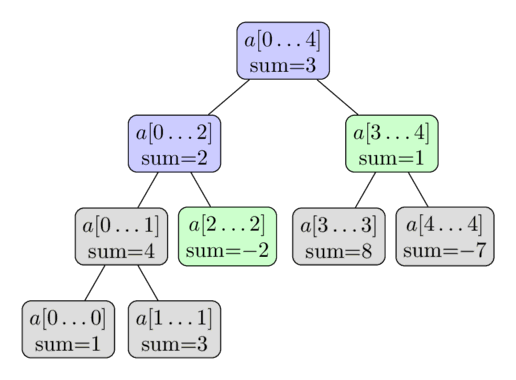
\includegraphics[width=8cm]{SLPUU.png}% Joonise suurus, joonise fail
    \caption{Massiivil $a[1,3,-2,8,-7]$ põhineva lõikude puu struktuur summapäringutele relevantselt värvituna}% Allkiri
    \allikas{Algorithms for Competitive Programming}% Allikas
    \label{joonislol}% Selle järgi viidatakse, pärast käsku \caption
\end{figure}

Miks on algoritmi ajaline keerukus $O(\log N)$? Sellepärast et igal tasemel külastame maksimaalselt $4$ tippu ja puu pikkus on $O(\log N)$ s.t kokku külastame maksimaalselt $4\log N$ tippu. \parencite{EMaxx}

Miks $4$? Esiteks kuni $4$ tasemeni puu tipust on teada et ei ole võimalik külastada ühel tasemel rohkem kui $4$ tippu sellepärast et tegu on kahendpuuga ehk tasemete tippude arvu saab kujutada geomeetrilise jadana ${1, 2, 4, 8, 16...}$. Edasistel tasemetel on põhjus selgitatav selle kaudu et päringus küsitakse pideva lõigu summat s.t et meil on teada et päringu lõik katab täielikult ära keskmised tipud ehk teise sõnaga võib päring jätkuda ainult kas kõige vasak- või parempoolsest tipust mitte mõlemast(!), ja need omakorda jagunevad maksimaalselt $4$ tipuks. See kõik mis on mainitud kehtib muidugi olukorras kus puu läbimine on otsustanud hargneda kaheks. \parencite{EMaxx}

Nüüd teiseks käsitleme niinimetatud uuendamispäringut kus me tahame lõikude puu kontekstis teha operatsiooni $a[i]=x$, kus x on mingi vabalt valitud täisarv, mis jääb andmetüübi piiridesse. \parencite{EMaxx}

Sellepärast et uuendada on vaja igal tasemel ainult ühte tippu ja juurtipu pikkus on $\log N$, on teada et ajakeerukus on $O(\log N)$.
On lihtne täheldada, et operatsiooni saab implementeerida rekursiivselt. Näiteks funktsioonile edastatakse juurtipp, ja rekursiivselt kutsub ennast välja ühel lapstipul, kuni lõpuni mingi puu leheni välja. Seejärel arvutatakse välja uuendatud puutippude väärtused. \parencite{EMaxx}


Üks olukord oleks näiteks selline kus toimub uuendus $a[2]=3$, joonisel rohelised tipud on need mida külastatakse ja uuendatakse.

\begin{figure}[H]% [] sisse märgitakse paigutus H
    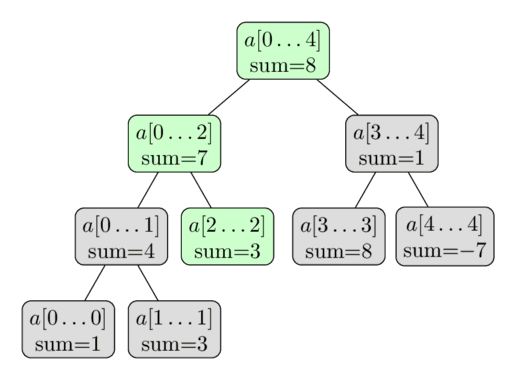
\includegraphics[width=8cm]{ULPUU.png}% Joonise suurus, joonise fail
    \caption{Massiivil $a[1,3,-2,8,-7]$ põhineva lõikude puu struktuur uuenduspäringutele relevantselt värvituna}% Allkiri
    \allikas{Algorithms for Competitive Programming}% Allikas
    \label{EMaxx}% Selle järgi viidatakse, pärast käsku \caption
\end{figure}

\section{Lõikude puu implementatsioon}

Alustame sellest et kuidas salvestada lõikude puud, kasutame selleks massiivi kuhu salvestame lõikude summad kujul kus juurtipu väärtus on salvestatud asukohal indeksiga $1$(kui alustada loendamist $1$-st), selle lapstippude väärtused on asukohtadel indeksiga $2$ ja $3$ jne. On lihtne täheldada et tipu $i$ vasakpoolne laps on asukohal indeksiga $2i$ ja parempoolne laps asukohal $2i+1$. \parencite{EMaxx}

Nagu enne mainitud on maksimaalne tippude arv $4N$, see tähendab et defineerime massiivi antud suurusega:
\begin{cclol}
// üldjuhul maksimaalne n suurus mida on ülesandes vaja
int MAXN = 2e5;
//
int t[4*MAXN];
\end{cclol}
\begin{kk}[H]% [] sisse märgitakse paigutus H
    \caption{Implementatsioon}% Allkiri
    \allikas{Autori implementatsioon}% Allikas
    \label{EMaxx}% Selle järgi viidatakse, pärast käsku \caption
    \end{kk}
Nüüd defineerime rekursiivse funktsiooni parameetritega, sisendmassiiv $a[]$, praegu vaadeldava tipu indeks $v$ ning praeguse lõigu piirelementide indeksid $tl$(vasakpoolne) ja $tr$(parempoolne).
\begin{cclol}
void build(int a[], int v, int tl, int tr) {
    if (tl == tr) {
        t[v] = a[tl];
    } else {
        int tm = (tl + tr) / 2;
        build(a, v*2, tl, tm);
        build(a, v*2+1, tm+1, tr);
        t[v] = t[v*2] + t[v*2+1];
    }
}
\end{cclol}
 \begin{kk}[H]% [] sisse märgitakse paigutus H
    \caption{Implementatsioon}% Allkiri
    \allikas{Algorithms for Competitive Programming}% Allikas
    \label{EMaxx}% Selle järgi viidatakse, pärast käsku \caption
    \end{kk}
Nagu on vajalik kutsutakse see funktsioon alustuseks juurtipu parameetritega: $v=1$, $tl=0$ ja $tr=n-1$.

Defineerime ka summapäringu funktsiooni, kus lisaks juurtipu parameetritele võtame sisendiks päritava lõigu piirid $l$ ja $r$.
\begin{cclol}
int sum(int v, int tl, int tr, int l, int r) {
    if (l > r) 
        return 0;
    if (l == tl && r == tr) {
        return t[v];
    }
    int tm = (tl + tr) / 2;
    return sum(v*2, tl, tm, l, min(r, tm))
           + sum(v*2+1, tm+1, tr, max(l, tm+1), r);
}
\end{cclol}
 \begin{kk}[H]% [] sisse märgitakse paigutus H
    \caption{Implementatsioon}% Allkiri
    \allikas{Algorithms for Competitive Programming}% Allikas
    \label{EMaxx}% Selle järgi viidatakse, pärast käsku \caption
    \end{kk}
Viimaseks toon välja uuenduspäringu kus lisaks juurtipu parameetritele võtame sisendiks muudetava elemendi positsiooni $pos$ ja elemendi uuendatud väärtuse $new$\textunderscore$val$.
\begin{cclol}
void update(int v, int tl, int tr, int pos, int new_val) {
    if (tl == tr) {
        t[v] = new_val;
    } else {
        int tm = (tl + tr) / 2;
        if (pos <= tm)
            update(v*2, tl, tm, pos, new_val);
        else
            update(v*2+1, tm+1, tr, pos, new_val);
        t[v] = t[v*2] + t[v*2+1];
    }
}
\end{cclol}
 \begin{kk}[H]% [] sisse märgitakse paigutus H
    \caption{Implementatsioon}% Allkiri
    \allikas{Algorithms for Competitive Programming}% Allikas
    \label{EMaxx}% Selle järgi viidatakse, pärast käsku \caption
    \end{kk}

\subsubsection{Ülesanded}
\begin{itemize}
    \item CSES - Dynamic Range Sum Queries(uurimistöö autori lahendus on peatükis 2.2.1.3., näidiskood iteratiivne(täpsemalt peatükis Iteratiivne implementatsioon))
    \item CSES - Range Update Queries(uurimistöö autori lahendus on peatükis 2.2.1.4., näidiskood iteratiivne(täpsemalt peatükis Iteratiivne implementatsioon))
    \item \href{https://codeforces.com/problemset/problem/356/A}{Codeforces - Knight Tournament(Keskmise raskusastmega(***))}
    \item Codeforces EDU - Nested Segments(uurimistöö autori lahendus on peatükis 2.2.2.5., näidiskood iteratiivne(täpsemalt peatükis Iteratiivne implementatsioon))
    \item Codeforces EDU - Intersecting segments(uurimistöö autori lahendus on peatükis 2.2.2.6., näidiskood iteratiivne(täpsemalt peatükis Iteratiivne implementatsioon))
    \item CSES - Subtree Queries(uurimistöö autori lahendus on peatükis 2.2.2.9., näidiskood rekursiivne)
    \item \href{https://cses.fi/problemset/task/1748}{CSES - Increasing Subsequence II(Suhteliselt raske(****))}
    \item Poola Informaatikaolümpiaad 2014 - Cards(uurimistöö autori lahendus on peatükis 2.2.2.11., näidiskood rekursiivne)
\end{itemize}
\subsection{Mälutõhus $build()$ implementatsioon}

Selles alapeatükis toon välja mälutõhusa implementatsiooni, kuigi enamus juhtudel on varem väljatoodud implementatsioon piisavalt vähese mälu nõudlusega(Codeforces-is enamasti sobib eelnev sest mälulimiidiks on $256$ MB).

Varasemad implementatsioonis kasutasime $O(4\cdot N)$ mälu, kuigi lõikude puu $N$ elemendiga massiivist vajab ainult $2N-1$ tippu. Sellest saab järeldada, et mõned indeksid jäävad puu ehitamisel kasutamata. \parencite{EMaxx}

Uues implementatsioonis nummerdame puu tipud Euleri ringreisi(inglise keeles Euler tour traversal, leiab infot ka nime pre-order traversal all) järjekorras ja kirjutame kõik tipud üksteise kõrvale(Lisa 3).

Vaatame tippu indeksiga $v$, mis vastutab lõigu $[l...r]$ eest, ning kasutame $mid =  \frac{l+r}{2}$. On lihtne täheldada et vasakpoolse lapse indeks on $v+1$, mis hoiab informatsiooni lõigu $[l, mid]$ kohta s.t $v+1$ alampuus on $2\cdot(mid-l+1)-1$ tippu. Seda teades saab leida $v$ parempoolse lapse indeksi valemiga $v+2\cdot(mid-l+1)$. \parencite{EMaxx}

Nende optimisatsioonide abil saame ruumikeerukuseks $O(2N)$, kus $N$ on tippude arv. \parencite{EMaxx}



\section{Lõikude puude omaduste laiendamine keeruliste päringute võimaldamiseks}

Selles peatükis käsitleme keerulisemaid päringuid, tähtis on täheldada, et paljud päringutüübid on oluliselt keerulisemad ja nõuavad programmeerijalt kõrgemat taset ja võib-olla on tegu liiga suure hüppega eelnevast peatükist.

\subsection{Maksimumi ja miinimumi leidmine lõigus}

Alustame maksimumi leidmisest mingis lõigus. Selle päringu võimaldamiseks ei ole vajalik lõikude puu tavapärase struktuuri muutmine, aga peame muutma kuidas arvutatakse $t[v]$ enne mainitud $build$(ehitamine) ja $update$(uuendus) funktsioonides. $t[v]$ nüüd salvestab vastava lõigu maksimaalse väärtuse ehk tipude väärtused on võrdsed mingi lõigu maksimumidega. Samuti peame muutma kuidas $sum$(summa) funktsioonis arvutatakse tagastatav väärtus(asendas summa arvutamise maksimaalse leidmisega). \parencite{EMaxx}

On lihtne märgata, et peaaegu samamoodi käib miinimumi leidmine. Veel saab leida sarnaselt suurima ühisteguri(edaspidi GCD/SÜT) ja vähima ühiskordse(edaspidi LCM/VÜK) lõikude kohta. 

Selle jaoks salvestame igas tipus relevantse GCD/LCM, ühendamine on võimalik mõlema tippu GCD/LCM leidmisega. \parencite{EMaxx}

\subsubsection{Ülesanded}
\begin{itemize}
    \item CSES - Dynamic Range Minimum Queries/Codeforces EDU - Segment tree for the minimum(uurimistöö autori lahendus on peatükis 2.2.1.1./2.2.1.2., näidiskood iteratiivne(täpsemalt peatükis Iteratiivne implementatsioon))
    \item Codeforces EDU - Number of minimums to segment(uurimistöö autori lahendus on peatükis 2.2.2.1., näidiskood iteratiivne(täpsemalt peatükis Iteratiivne implementatsioon))
    \item Codeforces EDU - Applying max on a segment(uurimistöö autori lahendus on peatükis 2.2.2.2., näidiskood rekursiivne)
    \item Codeforces EDU - Segment with the maximum sum(uurimistöö autori lahendus on peatükis 2.2.2.7., näidiskood rekursiivne)
\end{itemize}

\subsection{$0$-de hulga leidmine lõigus ja $k$-nda nulli indeksi leidmine}

Teine levinum kuid keerulisem päringu tüüp on $0$-de arvu leidmine mingis lõigus, alamülesandeks on $k$-nda nulli indeksi leidmine.
Seekord nagu arvata on massiivis $t$ salvestatud nullide arv mingi lõigu kohta. \parencite{EMaxx}

On lihtne täheldada, kuidas lahendada ülesande esimene osa kasutades ideid summapäringutest. Teise alamülesande -- $k$-nda nulli indeksi leidmine käib järgnevalt -- alustame juurtipust, liigume vasakule või paremale lapstipule olenevalt sellest kumba lõik sisaldab $k$-ndat nulli, et seda teada alustame sellest et vaatame mitut nulli sisaldab vasakpoolne lõik, kui see arv on suurem või võrdne $k$-ga siis järelikult valime vasakpoolse lapstipu kui mitte siis parempoolse. Tähtis on ka täheldada et kui valida parempoolne lapstipp peame lahutama vasakpoolse lõigu nullide arvu $k$-st. \parencite{EMaxx}

Järgnevas implementatsioonis tagastame $-1$ kui nullide arv terves massiivis on väiksem kui $k$. \parencite{EMaxx}
\begin{cclol}
int find_kth(int v, int tl, int tr, int k) {
    if (k > t[v])
        return -1;
    if (tl == tr)
        return tl;
    int tm = (tl + tr) / 2;
    if (t[v*2] >= k)
        return find_kth(v*2, tl, tm, k);
    else 
        return find_kth(v*2+1, tm+1, tr, k - t[v*2]);
}
\end{cclol}
 \begin{kk}[H]% [] sisse märgitakse paigutus H
    \caption{Implementatsioon}% Allkiri
    \allikas{Algorithms for Competitive Programming}% Allikas
    \label{EMaxx}% Selle järgi viidatakse, pärast käsku \caption
    \end{kk}

\subsubsection{Ülesanded}
\begin{itemize}
    \item Codeforces EDU - K-th one(uurimistöö autori lahendus on peatükis 2.2.2.3., näidiskood rekursiivne)
\end{itemize}

\subsection{Leiame lõigu prefiksi mille summa on suurem kui või võrdne \texorpdfstring{$x$}{TEXT}}
Järgmine päringutüüp on järgnev -- antud sisendiks täisarv $x$ peame me leidma väiksema indeksi $i$, mis rahuldab tingimust et esimese $i$ elemendi summa massiivis $a[]$ on võrdne või suurem kui $x$.

Ülesande saab lahendada kasutades kahendotsignut(inglise keeles binary search), kuid selle lahenduse ajakeerukus ei ole optimaalne($O(\log^2 N)$)\parencite{usaco}.

Teine variant on kasutada ideid eelmisest ülesandetüübist kasutades lõikude puud ning lahendada ülesanne ajakeerukusega $O(\log N)$. \parencite{EMaxx}

\subsubsection{Ülesanded}
\begin{itemize}
    \item Codeforces EDU - First element at least X(uurimistöö autori lahendus on peatükis 2.2.2.4., näidiskood rekursiivne)
    \item  \href{https://codeforces.com/edu/course/2/lesson/4/2/practice/contest/273278/problem/D}{Codeforces EDU - First element at least X - 2(Lihtne)}
\end{itemize}
\subsection{Esimese \texorpdfstring{$x$}{TEXT}-st suurema arvu indeksi leidmine vahemikus}
Viimane niimoodi lahendatav meie poolt käsitletav päringutüüp on järgnev -- antud täisarv $x$ ja vahemik massiivis $a[]$(täisarvude $l$ ja $r$ abil), leia vähim $i$ vahemikus $a[l...r]$ kus $a[i]$ on suurem kui $x$. 

Lihtsaim ja soovitatud lahendus ülesandele kasutab samat ideed mis eelmises ülesandes, lõikude puus liikudes vasakule või paremale olenevalt sellest mis on vasakpoolses lapstipus maksimaalne väärtus. Vastuse saame ajakeerukusega $O(\log N)$. \parencite{EMaxx}

\subsection{Salvestame lõigud puu tippudes}

Hulganisti lahendusi avaneb kasutades uut meetodit, salvestame lõigud täielikult puu tippudesse(inglise keeles Merge Sort Tree). Ruumikeerukus ja ajakeerukus on $O(N\log N)$. Lõigud saab omakorda jällegi lõikude puus salvestada vastavalt ülesandele mistahes andmestruktuuris. \parencite{EMaxx}

\subsubsection{Vähima arvu leidmine lõigus $a[l...r]$ mis on võrdne või suurem kui täisarv $x$}
Alguses peame implementeerima uutmoodi lõikude puu, selle jaoks, igasse tippu salvestame sorteeritud(suurenev) lõigu. Tegu on ideelt samasuguse rekursiivse funktsiooniga nagu varem kirjeldatud. 
Uutmoodi käib tippude ühendamine, selle jaoks on meil vaja ühendada kaks sorteeritud listi üheks, õnneks on C++ STL-s olemas implementatsioon sellest algoritmist nime $merge$ all. \parencite{EMaxx}

\begin{cclol}
vector<int> t[4*MAXN];

void build(int a[], int v, int tl, int tr) {
if (tl == tr) {
    t[v] = vector<int>(1, a[tl]);
} else { 
    int tm = (tl + tr) / 2;
    build(a, v*2, tl, tm);
    build(a, v*2+1, tm+1, tr);
    merge(t[v*2].begin(),t[v*2].end(),t[v*2+1].begin(),t[v*2+1].end(),
             back_inserter(t[v]));
}
}
\end{cclol}
 \begin{kk}[H]% [] sisse märgitakse paigutus H
    \caption{Implementatsioon}% Allkiri
    \allikas{Algorithms for Competitive Programming}% Allikas
    \label{EMaxx}% Selle järgi viidatakse, pärast käsku \caption
    \end{kk}
Mingis lõigus vähima arvu leidmine, mis vastab eelmainitud tingimusele, käib kahendotsingu abil seda võimaldab muidugi see, et lõik on sorteeritud.
Lihtne on ka täheldada et sisendlõik on jagatud mitmesse tippu, siis on vaja leida mõlemas leida sobiv arv ning seejärel leida miinimum nendest mõlemast.
Kahendotsingu ajakeerukus ühe lõigu peal on $O(\log N)$, millest saab järeldada et terve päringu ajakeerukus on $O(\log^2 N)$. \parencite{EMaxx}

Vastusfunktsiooni sisendiks saame lõigu piirindeksid $l$ ja $r$, massiivi $a[]$ ja täisarvu $x$.
\begin{cclol}
int query(int v, int tl, int tr, int l, int r, int x) {
if (l > r)
    return INF;
if (l == tl && r == tr) {
    vector<int>::iterator pos=lower_bound(t[v].begin(), t[v].end(), x);
    if (pos != t[v].end())
        return *pos;
    return INF;
}
int tm = (tl + tr) / 2;
return min(query(v*2, tl, tm, l, min(r, tm), x), 
            query(v*2+1, tm+1, tr, max(l, tm+1), r, x));
}
\end{cclol}
 \begin{kk}[H]% [] sisse märgitakse paigutus H
    \caption{Implementatsioon}% Allkiri
    \allikas{Algorithms for Competitive Programming}% Allikas
    \label{EMaxx}% Selle järgi viidatakse, pärast käsku \caption
    \end{kk}
$INF$ tähistab arvu mille väärtus on kindlasti suurem kui kõik väärtused massiivis.

\paragraph{Ülesanded}
\begin{itemize}
    \item \href{https://oj.uz/problem/view/COCI17_deda}{COCI - Deda(Suhteliselt raske(****))}
\end{itemize}

\paragraph{Optimeerimine murdosalise kaskaadiga}

Meetodit saab kiirendada ligikaudu ajakeerukuseni $O(\log N)$ kasutades tehnikat nimega murdosaline kaskaad(inglise keeles fractional cascading).

Lihtsamaks arusaamiseks alustame sellest, et selle asemel et teha kahendotsingut mitu korda, saaksime seda teha vaid üks kord, et seda võimaldada ühendame mitu sorteeritud listi üheks, salvestame ka mitmendal kohal oli element igas algnevas listis, kujul $x[i...i+k]$ kus $x$ on algse massiivi element, $i$ selle indeks algses massiivis ning $k$ on algsete massiivide arv. Sellel juhul oleks ruumikeerukus $O(kN)$, kus $N$ on ühendatud massiivi elementide arv. \parencite{EMaxx}

Murdosalise kaskaadiga saab vähendada selle ruumikeerukus $O(n)$-ni. Ajakeerukus on jätkuvalt veel $O(\log N+k)$. \parencite{cascade}

Võttega saab sarnaselt optimiseerida ka tavapärast iteratiivset otsingualgoritmi. \parencite{brown}

\subsection{Lõikude uuendamine, laisk laienemine}

Varasemalt käsitlesime uuenduspäringuid ainult ühel elemendil, kuid sama ajakeerukusega($O(\log N)$) võimaldab lõikude puu ka terve lõigu uuendamist. \parencite{EMaxx}

Alustame liitmisest, s.t peame liitma vahemikule $a[l...r]$ arvu $x$. Peaksime võimaldama ka vastamist päringule kujul: mis on $a[i]$ väärtus?

Et täita päringut efektiivselt, salvestame puu igasse relevantsesse tippu arvu $x$. Näiteks kui mul tuleb päring parameetritega $x=3$, $l=0$ ja $r=n-1$, siis peaksime salvestama juurtipus väärtuse $3$. \parencite{EMaxx}

Juhul kui tuleb päring mis küsib $a[i]$ väärtust, peame lihtsalt läbima puu ja liitma kõik arvud mida kohtame tee peal. \parencite{EMaxx}
\begin{cclol}
void build(int a[], int v, int tl, int tr) {
    if (tl == tr) {
        t[v] = a[tl];
    } else {
        int tm = (tl + tr) / 2;
        build(a, v*2, tl, tm);
        build(a, v*2+1, tm+1, tr);
        t[v] = 0;
    }
}

void update(int v, int tl, int tr, int l, int r, int add) {
    if (l > r)
        return;
    if (l == tl && r == tr) {
        t[v] += add;
    } else {
        int tm = (tl + tr) / 2;
        update(v*2, tl, tm, l, min(r, tm), add);
        update(v*2+1, tm+1, tr, max(l, tm+1), r, add);
    }
}

int get(int v, int tl, int tr, int pos) {
    if (tl == tr)
        return t[v];
    int tm = (tl + tr) / 2;
    if (pos <= tm)
        return t[v] + get(v*2, tl, tm, pos);
    else
        return t[v] + get(v*2+1, tm+1, tr, pos);
}
\end{cclol}
 \begin{kk}[H]% [] sisse märgitakse paigutus H
    \caption{Implementatsioon}% Allkiri
    \allikas{Algorithms for Competitive Programming}% Allikas
    \label{EMaxx}% Selle järgi viidatakse, pärast käsku \caption
    \end{kk}
Teine päringutüüp saaks olla selline kus soovitakse et omistaksime lõigu $a[l...r]$ iga elemendi mingile arvule väärtuse $p$. Nagu enne eeldame et võidakse ka küsida $a[i]$ väärtust. 

Et võimaldada seda on meil vaja salvestada iga puu tipus kas iga element massiivis on võrdne s.t et igas relevantses tipus on arv $p$. Sellest saab ka järeldada et terve alampuu sisaldab ka ainult seda arvu, jättes alampuu tippudele $p$ salvestamise ära(seda nimetatakse ka "laisaks" uuenduseks). \parencite{EMaxx}

Näiteks juhul kui saame päringu et omistaksime terve massiivi väärtusele $p$ siis märgime ära ainult juurtipu.\parencite{EMaxx}

Tähtis on täheldada, et juhul kui nüüd teine päring tahab et omistaksime lõigule $a[l...n/2]$ mingi muu väärtuse $x$, siis peaksime juure parempoolse lapse väärtuseks märkima $x$, aga vasakpoole lapse väärtuseks hoopis $p$. Seda saab teha niimoodi et kui juurele lisati väärtus $p$ lükkame selle väärtuse edasi ka selle lastele, ning eemaldame märke juurtipult, seejärel saame lihtsalt parempoolse lapse väärtuse muuta $x$-ks. \parencite{EMaxx}

Implementeerime $push()$ funktsiooni, mis tegeleb väärtuse lükkamisega lastele. Selle kutsume päringu alguses kõikidel tipudel peale lehtede. \parencite{EMaxx}
\begin{cclol}
void push(int v) {
    if (marked[v]) {
        t[v*2] = t[v*2+1] = t[v];
        marked[v*2] = marked[v*2+1] = true;
        marked[v] = false;
    }
}

void update(int v, int tl, int tr, int l, int r, int new_val) {
    if (l > r) 
        return;
    if (l == tl && tr == r) {
        t[v] = new_val;
        marked[v] = true;
    } else {
        push(v);
        int tm = (tl + tr) / 2;
        update(v*2, tl, tm, l, min(r, tm), new_val);
        update(v*2+1, tm+1, tr, max(l, tm+1), r, new_val);
    }
}

int get(int v, int tl, int tr, int pos) {
    if (tl == tr) {
        return t[v];
    }
    push(v);
    int tm = (tl + tr) / 2;
    if (pos <= tm) 
        return get(v*2, tl, tm, pos);
    else
        return get(v*2+1, tm+1, tr, pos);
}
\end{cclol}
 \begin{kk}[H]% [] sisse märgitakse paigutus H
    \caption{Implementatsioon}% Allkiri
    \allikas{Algorithms for Competitive Programming}% Allikas
    \label{EMaxx}% Selle järgi viidatakse, pärast käsku \caption
    \end{kk}
*Implementatsiooni saab mõnevõrra loogilisemaks muuta, kasutades tõeväärtustega massiivi.

\subsubsection{Ülesanded}
\begin{itemize}
    \item \href{https://codeforces.com/problemset/problem/446/C}{Codeforces - DZY Loves Fibonacci Numbers(Raske(****))}
    \item \href{https://codeforces.com/edu/course/2/lesson/5/2/practice/contest/279653/problem/C}{Codeforces EDU - Bitwise OR and AND(Lihtne(**))}
    \item Eesti Informaatikaolümpiaad 2022/2023 II valikvõistlus - Kaardid(uurimistöö autori lahendus on peatükis 2.2.2.8., rekursiivne)
    \item USACO Platinum - Counting Haybales(uurimistöö autori lahendus on peatükis 2.2.2.10., rekursiivne)
\end{itemize}

\subsection{Kõrgematele dimensioonidele üldistamine}

Laiendamine on teoreetiliselt üsnagi lihtne, lõikude puu salvestab lõikude asemel veel järgmisi lõikude puid.

\subsubsection{2D lõikude puu}
Sisendiks saame maatriksi $a[0...n-1][0...m-1]$, ja proovime leida mingi alammaatriksi $a[x_1...x_2][y_1...y_2]$ summa ja võimaldada päringuid kujul $a[x][y]=p$.
Alguses lihtsalt defineerime lõikude puu $x$ koordinaadi abil, siis sellepärast et $x$ koordinaat on juba seotud lõiguga $[l...r]$, s.t et töötame ribaga $a[l...r][0...m-1]$, selle alusel rajamegi järgmise lõikude puu. Väiksemad puud rajame $y$ koordinaadi alusel(võib ka muidugi vastupidi teha). \parencite{EMaxx}

Abijoonistel on tähtis teada et ülesannet on alustatud hoopis $y$ koordinaatidega puu loomisest\parencite{CPH}.
\begin{figure}[H]% [] sisse märgitakse paigutus H
    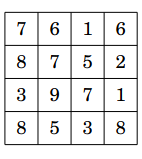
\includegraphics[width=5cm]{maatriks.png}% Joonise suurus, joonise fail
    \caption{Maatriks}% Allkiri
    \allikas{Competitive Programmer’s Handbook}% Allikas
    \label{CPH}% Selle järgi viidatakse, pärast käsku \caption
\end{figure}

\begin{figure}[H]% [] sisse märgitakse paigutus H
    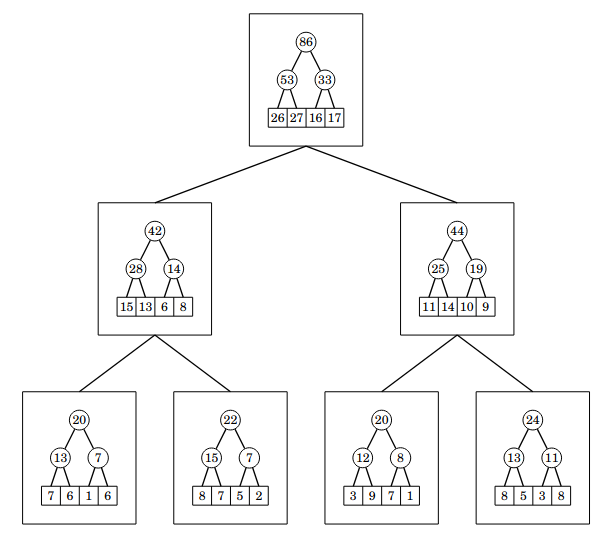
\includegraphics[width=16cm]{2DLPUU.png}% Joonise suurus, joonise fail
    \caption{2D lõikude puu maatriksi põhjal}% Allkiri
    \allikas{Competitive Programmer’s Handbook}% Allikas
    \label{CPH}% Selle järgi viidatakse, pärast käsku \caption
\end{figure}

\paragraph{Ülesanded}
\begin{itemize}
    \item \href{https://codeforces.com/problemset/problem/869/E}{Codeforces - The Untended Antiquity(Raske(****))}
    \item Rahvusvaheline Informaatikaolümpiaad 2013 - Game(vt peatükk 2.2.2.14.)
\end{itemize}
\subsection{Jäädvustav lõikude puu}
Jäädvustavaks andmestruktuuriks nimetatakse andmestruktuuri mis mäletab pärast muutmist ikka veel eelmiseid parameetreid \parencite{opik}.

Lõikude puus tahame vältida terve puu kopeerimist pärast igat modifikatsiooni, aga samaaeg soovime säilitada $O(\log N)$ ajakeerukuse lõigupäringuid tehes. \parencite{EMaxx}

On teada et, iga uuenduspäring lõikude puus põhjustab ainult $O(\log N)$ tippude muutmist alates juurtipust. 
Kui salvestame lõikude puu viitadena(inglise keeles pointers), siis selle asemel et muuta tippude väärtusi teeme lihtsalt uued tipud. Nüüd teame et, iga uuenduspäringuga peame looma $O(\log N)$ uut tippu, kaasa arvatud juurtipu.
\parencite{EMaxx}
\begin{cclol}
struct Vertex {
    Vertex *l, *r;
    int sum;

    Vertex(int val) : l(nullptr), r(nullptr), sum(val) {}
    Vertex(Vertex *l, Vertex *r) : l(l), r(r), sum(0) {
        if (l) sum += l->sum;
        if (r) sum += r->sum;
    }
};

Vertex* build(int a[], int tl, int tr) {
    if (tl == tr)
        return new Vertex(a[tl]);
    int tm = (tl + tr) / 2;
    return new Vertex(build(a, tl, tm), build(a, tm+1, tr));
}

int get_sum(Vertex* v, int tl, int tr, int l, int r) {
    if (l > r)
        return 0;
    if (l == tl && tr == r)
        return v->sum;
    int tm = (tl + tr) / 2;
    return get_sum(v->l, tl, tm, l, min(r, tm))
         + get_sum(v->r, tm+1, tr, max(l, tm+1), r);
}

Vertex* update(Vertex* v, int tl, int tr, int pos, int new_val) {
    if (tl == tr)
        return new Vertex(new_val);
    int tm = (tl + tr) / 2;
    if (pos <= tm)
        return new Vertex(update(v->l, tl, tm, pos, new_val), v->r);
    else
        return new Vertex(v->l, update(v->r, tm+1, tr, pos, new_val));
}
\end{cclol}
 \begin{kk}[H]% [] sisse märgitakse paigutus H
    \caption{Implementatsioon}% Allkiri
    \allikas{Algorithms for Competitive Programming}% Allikas
    \label{EMaxx}% Selle järgi viidatakse, pärast käsku \caption
    \end{kk}
Et kiiresti liikuda erinevate juurtippude vahel salvestame need massiivi.
Kirjeldatud meetodi abil saab peaaegu igas olukorras luua jäädvustav andmestruktuur. 

Jäädvustava lõikude puu $modify()$ funktsioon kasutab $O(\log N)$ mälu.

\subsubsection{Ülesanded}
\begin{itemize}
    \item \href{https://www.spoj.com/problems/KQUERY/}{SPOJ - KQUERY(Keskmise raskusastmega}
\end{itemize}
\subsubsection{$k$-da väikseima numbri leidmine lõigus}

$k$-da väikseima numbri leidmist lõigus saab võimaldada ka lihtsalt kahendotsingu ja ennem käsitletud tehnika abil (kus lõikude puus salvestame nt terved massiivi vahemikud), kuid siis oleks ajakeerukus iga päringu kohta $O(\log^3 N)$, mis on suboptimaalne. \parencite{EMaxx}

Lahendades ülesande jäädvustava lõikude puuga saame ühe päringu ajakeerukuseks $O(\log N)$. \parencite{EMaxx}

Et toetada arusaamist, alustame lihtsamast olukorrast: käsitleme ainult massiive, kus kehtib tingimus $0 \leq a[i] < N$, ning tahame ainult leida $k$-ndat väikseimat elementi mingis $a$ prefiksis. 

Kasutame $a$ jaoks 1-põhist indekseerimist.

Lõikude puu loendab kõik nähtud numbrid, s.t et lõikude puus salvestame justkui massiivi histogrammi. 
Puu lehtedes salvestame kui tihti väärtused $O...N-1$ ilmuvad massiivis, ülejäänud tipud salvestavad kui palju numbreid mingis vahemikus on massiivis.  \parencite{EMaxx}

Teisisõnu teeme tavapärase lõikude puu koos summapäringutega üle massiivi histogrammi.

Aga selle asemel et teha $N$ lõikude puud iga prefiksi kohta, loome ühe jäädvustava lõikude puu.

Alguses on meil tühi lõikude puu(kõik väärtused on $0$), millele suunab $root_0$, ja lisame elemendid $a[1]...a[N]$ järjest. Iga modifikatsiooniga saame uue juurtipu, kutsume $root_i$(puu juur pärast esimese $i$ elemendi lisamist).
Lõikude puu juurega $root_i$, sisaldab histogrammi $a[1...i]$. Nagu enne mainitud töötab see meetod ajakeerukusega $O(\log N)$. \parencite{EMaxx}

Nüüd käsitleme lühidalt igal tingimusel töötavat implementatsiooni, kus lõikude puu esindab histogrammi elementidest vahemikus $[l...r]$.
Nüüd saab iga tipp $[l...r]$ olema võrdne $root_r$ puu tipu ja $root_l-1$ tipu vahega.

Siin on modifitseeritud $build$, $update$, ja $find \_ kth$ funktsioonid:
\begin{cclol}
Vertex* build(int tl, int tr) {
    if (tl == tr)
        return new Vertex(0);
    int tm = (tl + tr) / 2;
    return new Vertex(build(tl, tm), build(tm+1, tr));
}

Vertex* update(Vertex* v, int tl, int tr, int pos) {
    if (tl == tr)
        return new Vertex(v->sum+1);
    int tm = (tl + tr) / 2;
    if (pos <= tm)
        return new Vertex(update(v->l, tl, tm, pos), v->r);
    else
        return new Vertex(v->l, update(v->r, tm+1, tr, pos));
}

int find_kth(Vertex* vl, Vertex *vr, int tl, int tr, int k) {
    if (tl == tr)
        return tl;
    int tm = (tl + tr) / 2, left_count = vr->l->sum - vl->l->sum;
    if (left_count >= k)
        return find_kth(vl->l, vr->l, tl, tm, k);
    return find_kth(vl->r, vr->r, tm+1, tr, k-left_count);
}
\end{cclol}
\begin{kk}[H]% [] sisse märgitakse paigutus H
    \caption{Implementatsioon}% Allkiri
    \allikas{Algorithms for Competitive Programming}% Allikas
    \label{EMaxx}% Selle järgi viidatakse, pärast käsku \caption
    \end{kk}

Järgnev on jäädustava lõikude puu implementatsioon, massiivi $a$ peal, elementidega vahemikus $[0...MAX \_ VALUE]$:
\begin{cclol}
int tl = 0, tr = MAX_VALUE + 1;
std::vector<Vertex*> roots;
roots.push_back(build(tl, tr));
for (int i = 0; i < a.size(); i++) {
    roots.push_back(update(roots.back(), tl, tr, a[i]));
}

//find the 5th smallest number 
//from the subarray [a[2], a[3], ..., a[19]]
int result = find_kth(roots[2], roots[20], tl, tr, 5);
\end{cclol}
\begin{kk}[H]% [] sisse märgitakse paigutus H
    \caption{Implementatsioon}% Allkiri
    \allikas{Algorithms for Competitive Programming}% Allikas
    \label{EMaxx}% Selle järgi viidatakse, pärast käsku \caption
    \end{kk}

Seoses massiivi elementidele seatud piirangutega: tegelikult saame kasutada igat massiivi ühe võtte abil(inglise keeles index compression). Väikseimale elemendile massiivis seadistame väärtuse $0$, järgmisele $1$ jne. Saame kasutada nt $map$(nt C++ või Python) andmestruktuuri, mis konverteerib väärtuse selle indeksiks või vastupidi ajakeerukusega $O(\log N)$.


\subsection{Dünaamiline lõikude puu} 
Peamine idee seisneb selles et selle asemel et salvestada kõik tipud loome tippe ainult siis kui vaja.
Ülesannetes kus päringu lõik on maksimaalselt $10^6$ on tavaline lõikude puu täitsa sobilik aga kui seda arvu ületada siis on tulemuseks $MLE$(Memory Limit Exceeded), siis peaksime kasutama dünaamilist lõikude puud.
Optimisatsioon seisneb uues ruumikeerukuses $O(M\log N)$, kus $N$ on tippude arv ja $M$ päringute hulk. Päringukeerukus on ikkagi $O(\log N)$. \parencite{EMaxx}

Järgnevas implementatsioonis võimaldame kahte päringutüüpi, positsioonile väärtuse liitmine(algselt kõik 0) ja mingis vahemikus kõikide arvude summa leidmine. \parencite{EMaxx}
Puu juureks on $Vertex(0, N)$.
\begin{cclol}
struct Vertex {
    int left, right;
    int sum = 0;
    Vertex *left_child = nullptr, *right_child = nullptr;

    Vertex(int lb, int rb) {
        left = lb;
        right = rb;
    }

    void extend() {
        if (!left_child && left + 1 < right) {
            int t = (left + right) / 2;
            left_child = new Vertex(left, t);
            right_child = new Vertex(t, right);
        }
    }

    void add(int k, int x) {
        extend();
        sum += x;
        if (left_child) {
            if (k < left_child->right)
                left_child->add(k, x);
            else
                right_child->add(k, x);
        }
    }

    int get_sum(int lq, int rq) {
        if (lq <= left && right <= rq)
            return sum;
        if (max(left, lq) >= min(right, rq))
            return 0;
        extend();
    return left_child->get_sum(lq, rq) + right_child->get_sum(lq, rq);
    }
};
\end{cclol}
 \begin{kk}[H]% [] sisse märgitakse paigutus H
    \caption{Implementatsioon}% Allkiri
    \allikas{Algorithms for Competitive Programming}% Allikas
    \label{EMaxx}% Selle järgi viidatakse, pärast käsku \caption
    \end{kk}
Laiendada võimalusi on ka muidugi võimalik, nagu nt lisades lõikude uuendamise päringu võimalus, laisa laienemise(inglise keeles lazy propagation) abil.

\subsubsection{Ülesanded}
\begin{itemize}
    \item \href{https://oj.uz/problem/view/IZhO12_apple}{IZHO 2012 - Monkey and Apple-Trees(Keskmise raskusastmega)}
    \item \href{https://oj.uz/problem/view/Balkan15_HAPPINESS}{Balkan OI 2015 - Happiness(Raske)}
    \item \href{https://dmoj.ca/problem/ioi05p3}{IOI 2005 - Mountain(Raske)}
\end{itemize}
\section{Iteratiivne implementatsioon} 
Iteratiivne implementatsioon on tihti eelistatud põhjusel, et see võib väiksema konstandi tõttu olla oluliselt kiirem, näiteks kui mõlema lähenemise ajakeerukus on $O(1)$ siis peaaegu alati on rekursiivne lahendus ikkagi ressurssikulukam/aeglasem.
Enamik eelistab siiski rekursiivset implementatsiooni põhjusel, et see on levinum, ning loogilisem(see on subjektiivne, ning autor on vastupidisel arvamusel).

\subsection{Lõigul summa leidmine ja elemendi väärtuse uuendamine}

\begin{figure}[H]% [] sisse märgitakse paigutus H
    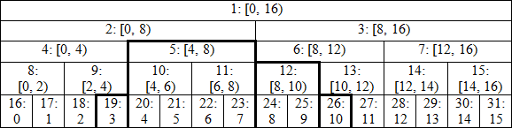
\includegraphics[width=12cm]{LIHTPUU.png}% Joonise suurus, joonise fail
    \caption{}% Allkiri
    \allikas{Codeforces. Efficient and easy segment trees}% Allikas
    \label{joonis}% Selle järgi viidatakse, pärast käsku \caption
\end{figure}
Jooniselt on näha et puu üldine struktuur on sama mis uurimistöö varasemates peatükkides kasutusel, kuid eeldame praegu et massiivi pikkus on kahe aste s.t et saame perfektse lõikude puu. Näiteks juhul kui peame leidma vastuse summapäringule intervalil $[3...11)$, siis liidame tippude $19$, $5$, $12$ ja $26$(märgitud paksus kirjas) väärtused. \parencite{cfpuu}

NB! Kasutamine intervali notatsiooni $[)$ s.t et intervali $[l...r)$ juhul räägime lõigust, mis algab $l$-st(kaasaarvatud) ja lõppeb $r-1$-ga(kaasaarvatud). Indekseerimine on 0-põhine.

\begin{cclol}
const int N = 1e5;  // limit for array size
int n;  // array size
int t[2 * N];

void build() {  // build the tree
  for (int i = n - 1; i > 0; --i) t[i] = t[i<<1] + t[i<<1|1];
}

void modify(int p, int value) {  // set value at position p
  for (t[p += n] = value; p > 1; p >>= 1) t[p>>1] = t[p] + t[p^1];
}

int query(int l, int r) {  // sum on interval [l, r)
  int res = 0;
  for (l += n, r += n; l < r; l >>= 1, r >>= 1) {
    if (l&1) res += t[l++];
    if (r&1) res += t[--r];
  }
  return res;
}

int main() {
  scanf("%d", &n);
  for (int i = 0; i < n; ++i) scanf("%d", t + n + i);
  build();
  modify(0, 1);
  printf("%d\n", query(3, 11));
  return 0;
}
\end{cclol}
 \begin{kk}[H]% [] sisse märgitakse paigutus H
    \caption{Iteratiivse lõikude puu põhifunktsioonid}% Allkiri
    \allikas{Efficient and easy segment trees}% Allikas
    \label{cfpuu}% Selle järgi viidatakse, pärast käsku \caption
    \end{kk}

Implementatsioon on lahti seletatud kolmes osas:
\begin{enumerate}
    \item Puu lehed on salvestatud pidevalt alustades indeksiga $N$, element indeksiga $i$ vastab puus tipule indeksiga $i+N$.
    \item Puu ehitamisel, sellepärast et vanemtipu indeks on alati suurem kui lapstipu indeks, saame tippe töödelda kahanevad järjekorras. Bititehe funktsioonis $build()$ on võrdne operatsiooniga $t[i] = t[2\cdot i] + t[2\cdot i+1]$.
    \item Uuenduspäringu korral liigume puust üles, teades et tipu $p$ vanemtipp on $p/2$($p>>1$), bititehe $p^1$ võimaldab liikuda lapstippude indeksite $2\cdot i$ ja $2\cdot i+1$ vahel.
\end{enumerate}
\parencite{cfpuu}

Peamine idee on järgmine -- kui $l$, intervali vasakpoolne piir, on paaritu($l\&1$) järelikult $l$ on tipu parempoolne laps. Siis meie interval sisaldab tipp $l$-i aga mitte selle vanemat. Lisame seejärel $t[l]$-i ja liigume $l$-i vanemast paremale assigneerides $l=(l+1)/2$, kui $l$ on paarisarv, on tegu vasakpoolse lapsega ja interval sisaldab ka vanemat(kui parempoolne piir ei takista), siis me lihtsalt liigutame seda tehes operatsiooni $l=l/2$. Sarnaselt teeme parempoolse piiriga. Lõpetame kui piirid kohtuvad. \parencite{cfpuu}

Autor koostas ka joonise intervalil $[1, 6)$ tehtud operatsiooni kohta, kus punasega märgitud tipud jäävad lõigust välja(kuid on külastatud), lillad ja rohelised moodustavad lõigu:
\begin{figure}[H]% [] sisse märgitakse paigutus H
    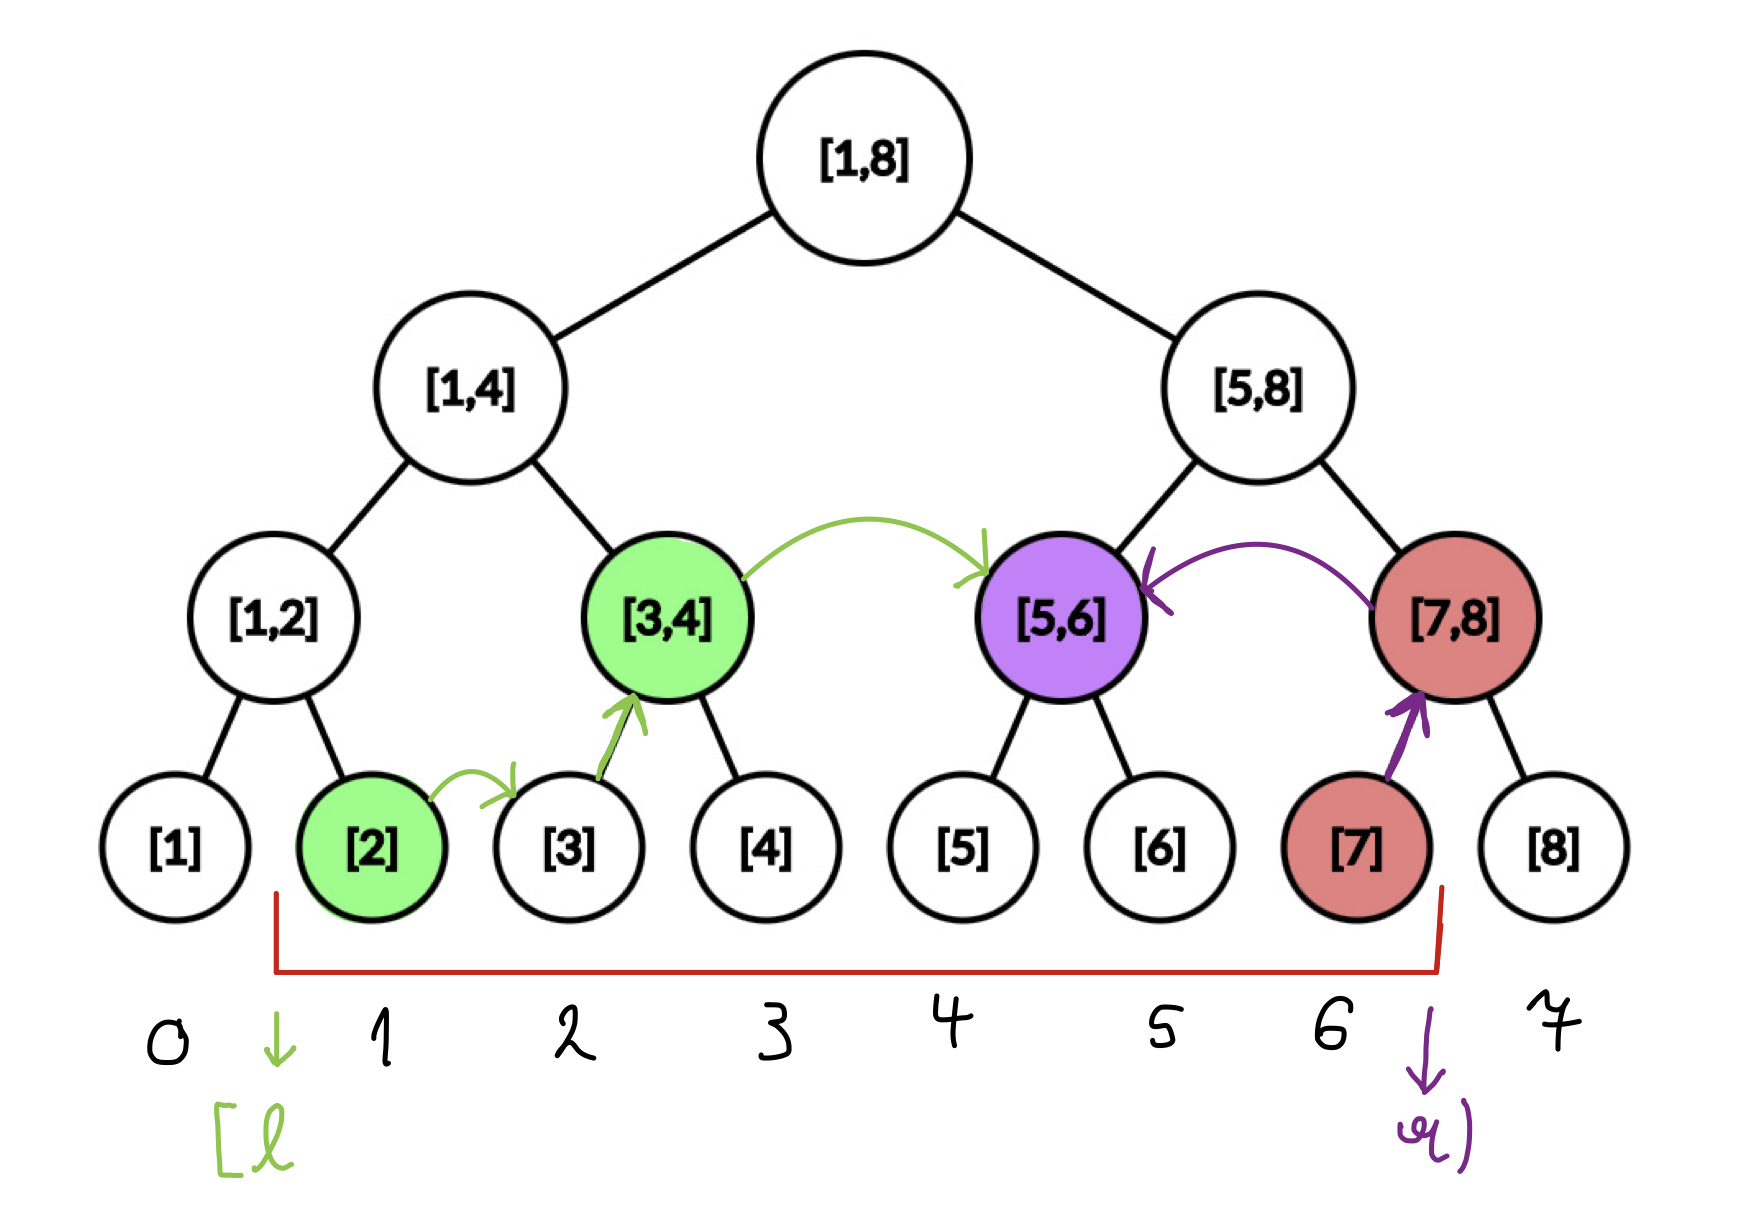
\includegraphics[width=12cm]{jonis2.png}% Joonise suurus, joonise fail
    \caption{Päring parameetritega 1 ja 6}% Allkiri
    \allikas{Autori koostatud joonis CS Academy ja GoodNotes abil}% Allikas
    \label{joonis}% Selle järgi viidatakse, pärast käsku \caption
\end{figure}


On huvitav täheldada, et kood töötab ka kui $N$ on paaritu. \parencite{cfpuu}
Sellel juhul on kuigi selgitus palju keerulisem. 
Puu parameetriga $n=13$ on kujutatud järgnevalt:
\begin{figure}[H]% [] sisse märgitakse paigutus H
    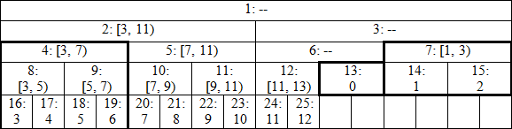
\includegraphics[width=12cm]{LIHTPUU2.png}% Joonise suurus, joonise fail
    \caption{}% Allkiri
    \allikas{Codeforces. Efficient and easy segment trees}% Allikas
    \label{joonis}% Selle järgi viidatakse, pärast käsku \caption
\end{figure}

Tegu sellisel juhul ei ole kuigi enam ühe puuga, vaid mitme perfektse kahendpuuga: juur $2$ ja kõrgus $4$, juur $7$ ja kõrgus $2$, juur $12$ ja kõrgus $2$, juur $13$ ja kõrgus $1$. 
Arusaama toetamiseks toon välja näidispäringu -- olgu meil antud interval $[0...7)$ ja parameetrid $l=13$, $r=20$. Teeme operatsiooni $l\&1 => add\_t[13]$ ning piirid muutuvad $l=7$, $r=10$. Seejärel teeme $l\&1 => add\_t[7]$, saame $l=4$, $r=5$ ja selle tagajärjel on tipud samal kõrgusel. Peale seda saame $r\&1 => add\_t[4 = --r]$ ja $l=2$, $r=2$ s.t. et algoritm on lõpetanud oma töö edukalt. \parencite{cfpuu}

Veel üks iteratiivne ja samal loogikal põhinev implementatsioon, kui ei taha bititehetega tegeleda on järgnev:
\begin{cclol}
int sum(int a, int b) {
a += n; b += n;
int s = 0;
while (a <= b) {
if (a%2 == 1) s += tree[a++];
if (b%2 == 0) s += tree[b--];
a /= 2; b /= 2;
}
return s;
}

void add(int k, int x) {
k += n;
tree[k] += x;
for (k /= 2; k >= 1; k /= 2) {
tree[k] = tree[2*k]+tree[2*k+1];
}
\end{cclol}
 \begin{kk}[H]% [] sisse märgitakse paigutus H
    \caption{Implementatsioon}% Allkiri
    \allikas{Competitive Programmer’s Handbook}% Allikas
    \label{CPH}% Selle järgi viidatakse, pärast käsku \caption
    \end{kk}

\subsection{Lõigule väärtuse liitmine ja elemendi väärtuse leidmine}
Mainitud operatsioone saab ka teha laisa laienemisega, kuid praegusel juhul ei ole see tegelikult vajalik.

Peame lihtsalt modifitseerima varem käsitletud funktsioone:
\begin{cclol}
void modify(int l, int r, int value) {
  for (l += n, r += n; l < r; l >>= 1, r >>= 1) {
    if (l&1) t[l++] += value;
    if (r&1) t[--r] += value;
  }
}

int query(int p) {
  int res = 0;
  for (p += n; p > 0; p >>= 1) res += t[p];
  return res;
}
\end{cclol}
\begin{kk}[H]% [] sisse märgitakse paigutus H
    \caption{Implementatsioon}% Allkiri
    \allikas{Efficient and easy segment trees}% Allikas
    \label{CPH}% Selle järgi viidatakse, pärast käsku \caption
    \end{kk}

On tähtis täheldada, et algselt, enne modify operatsiooni on puus kõikide tippude peale lehtede väärtused $0$.

Kui mingil hetkel pärast muudatusi on meil vaja kontrollida kõiki massiivi elemente, saame muudatused lükata lehtedele, kasutades allpool olevat koodi. Pärast seda saame lihtsalt läbida elemente alates indeksist $N$. Keerukus $O(N_logN)$ asemel $O(N)$, sarnasel põhjusel, kui teha $N$ muudatuse asemel $build()$.

\begin{cclol}
void push() {
  for (int i = 1; i < n; ++i) {
    t[i<<1] += t[i];
    t[i<<1|1] += t[i];
    t[i] = 0;
  }
}
\end{cclol}
\begin{kk}[H]% [] sisse märgitakse paigutus H
    \caption{Implementatsioon}% Allkiri
    \allikas{Efficient and easy segment trees}% Allikas
    \label{CPH}% Selle järgi viidatakse, pärast käsku \caption
    \end{kk}
On tähtis täheldada, et sedasorti kood töötab ainult juhul kui operatsioonid on kommutatiivsed, ehk operatsioonide järjekorrast ei olene tulemus.

Sobivad operatsioonide kombinatsioonid on näiteks:
\begin{table}[H]
\caption{Sobivad operatsioonid}% Pealkiri
\label{tabel2}% Tabelile viitamine
\scalebox{1}{
\begin{tabular}
{r|r}% r - paremjoondatud tulp, | - püstjoon
\hline% Horisontaalne joon
Uuendamine & Leidmine\\
\hline
Korrutamine & Liitmine\\
Liitmine & min/max leidmine\\
AND operatsioon & OR operatsioon\\
\hline
\end{tabular}
}
\allikas{Autori kogutud andmed}% Viide
\end{table}

Kui see omadus ei ole rahuldatud siis peame kasutama laiska uuendamist.
\subsection{Laisk laienemine} 
Laisk laienemine võimaldab ka mittekomutatiivseid operatsioone.
Esiteks, meil on vaja lisaks veel ühte muutujat ja massiivi:
\begin{cclol}
int h = sizeof(int) * 8 - __builtin_clz(n);
int d[N];  
\end{cclol}
\begin{kk}[H]% [] sisse märgitakse paigutus H
    \caption{Implementatsioon}% Allkiri
    \allikas{Efficient and easy segment trees}% Allikas
    \label{CPH}% Selle järgi viidatakse, pärast käsku \caption
    \end{kk}
$h$ on puu kõrgus, ehk 'most significant bit' muutujas $n$. $d[]$ on massiiv mis on peaaegu identne koopia massiivist $t[]$, ainust erinevus seisneb sellest, et ei salvesta puulehti, tänu millele on vaja defineerida ainult $N$ suurusega massiiv(lisaks massiivile $t[]$).

Enne saime väita, et $t[i]$ salvestab endas alati kõige viimatisemat informatsiooni lõigu $i$ kohta. Laisa laienemisega peame korrektsete andmete saamiseks enne seda uuendama lõigu andmeid, seda teeme liikudes tipust $i$ kuni juurtipuni. Eeldame, et $t[i]$ sisaldab juba $d[i]$, nii et alustame mitte $i$-st, vaid selle otsesest vanemast.

Tulles tagasi esimese näite juurde, kus on intervall $[3, 11)$, kuid nüüd tahame muuta kõiki selle intervalli sees olevaid elemente. Selleks muudame $t[i]$ ja $d[i]$ tippudes $19$, $5$, $12$ ja $26$. Hiljem, kui meilt küsitakse väärtust näiteks tipus $22$, peame muutusi propageerima tipust $5$ mööda puud alla. Pange tähele, et meie muudatused võivad mõjutada $t[i]$ väärtusi ka ülevalpool puul: tippu $19$ mõjutavad tipud $9$, $4$, $2$ ja $1$, tippu $5$ mõjutavad $2$ ja $1$. Järgmine asjaolu on meie operatsioonide ajalise keerukuse seisukohalt tähtis:

Muutmine intervalil $[l, r)$ mõjutab massiivi $t[]$ väärtusi ainult ääre lehtede vanemates: $l+n$ and $r+n-1$.

Millest on see põhjustatud? Vasakpoolse serva töötlemisel on tipp, mida me oma tsüklis muudame, alati selle vanema parempoolne laps. Siis on kõik eelnevad muudatused tehtud sama vanema vasakpoolse lapse alampuule. Vastasel juhul töötleksime mõlema lapse asemel vanemat. See tähendab, et praegune otsene vanem on ka lehe $l+n$ vanem. Samasugused argumendid kehtivad ka parempoolse ääre kohta.


Järgnev koodilõik näitab ära kuidas kasutada eelnevaid ideid, et teha lõigul liitmise ja lõigul maksimumi leidmise operatsioone samal puul.

\begin{cclol}
void apply(int p, int value) {
  t[p] += value;
  if (p < n) d[p] += value;
}

void build(int p) {
  while (p > 1) p >>= 1, t[p] = max(t[p<<1], t[p<<1|1]) + d[p];
}

void push(int p) {
  for (int s = h; s > 0; --s) {
    int i = p >> s;
    if (d[i] != 0) {
      apply(i<<1, d[i]);
      apply(i<<1|1, d[i]);
      d[i] = 0;
    }
  }
}

void inc(int l, int r, int value) {
  l += n, r += n;
  int l0 = l, r0 = r;
  for (; l < r; l >>= 1, r >>= 1) {
    if (l&1) apply(l++, value);
    if (r&1) apply(--r, value);
  }
  build(l0);
  build(r0 - 1);
}

int query(int l, int r) {
  l += n, r += n;
  push(l);
  push(r - 1);
  int res = -2e9;
  for (; l < r; l >>= 1, r >>= 1) {
    if (l&1) res = max(res, t[l++]);
    if (r&1) res = max(t[--r], res);
  }
  return res;
}
\end{cclol}
\begin{kk}[H]% [] sisse märgitakse paigutus H
    \caption{Implementatsioon}% Allkiri
    \allikas{Efficient and easy segment trees}% Allikas
    \label{CPH}% Selle järgi viidatakse, pärast käsku \caption
    \end{kk}
Vaatleme funktsioone ühekaupa:
\begin{enumerate}
   \item apply funktsioon uuendab nn laisa puu ja ka tavapuu väärtusi. $p<n$ abil kontrollime et $p$ ei oleks leht.

   \item $build$ funktsioon uuendab kõiki mingi tipu vanemaid.

   \item $push$ funktsioon lükkab/uuendab muutused juurtipust alla tipu $p$-ni. Vanemad on $p$ prefiksid kahendsüsteemis.

   \item $inc$ funktsioon liidab lõigule mingi väärtuse, uuendades laisa uuendamise meetodi kohaselt seda mis vaja.

   \item $query$ funktsioon leiab maksimum lõigul, kuid enne seda uuendab massiivis $t[]$ vajalike andmeid. Piisab push funktsiooni kasutamisest ääre tippude otsestel vanematel.

\end{enumerate}
Kõikide funktsioonide ajakeerukus on $O(\log N)$.

See on kuigi lihtsaim näide põhjustel, et:
\begin{enumerate}
   \item Operatsioonid on kommutatiivsed.
   \item Tipu uuendamisel ei vaja teade, et millisele intervalile see vastab.
\end{enumerate}

\subsubsection{Elemendi väärtuse uuendamine ja lõigul summa leidmine}
Järgmises näites käsitleme olukorda, kus need tingimused ei ole täidetud.
Alustame väärtuse muutmisest ja summa leidmisest.

Võtame kasutusele kaks uut funktsiooni:
\begin{cclol}
void calc(int p, int k) {
  if (d[p] == 0) t[p] = t[p<<1] + t[p<<1|1];
  else t[p] = d[p] * k;
}

void apply(int p, int value, int k) {
  t[p] = value * k;
  if (p < n) d[p] = value;
}
\end{cclol}
\begin{kk}[H]% [] sisse märgitakse paigutus H
    \caption{Implementatsioon}% Allkiri
    \allikas{Efficient and easy segment trees}% Allikas
    \label{CPH}% Selle järgi viidatakse, pärast käsku \caption
    \end{kk}
Need on lihtsad $O(1)$ funktsioonid et arvutada väärtus tipul $p$ ja teha muutusi. 

Autor selgitab paari muutust järgnevalt:
\begin{enumerate}
   \item Kontrollime, et $d[p] = 0$. Selle saab asendada tõeväärtustega massiiviga.

   \item Meil on uus parameeter $k$, mis tähistab tipule $p$ vastava intervali pikkust.
\end{enumerate}

Peame muutma ka $build$ ja $push$ funktsioone. Kombineerime varasemalt käsitletud funktsioonide funktsionaalsust:
\begin{cclol}
void build(int l, int r) {
  int k = 2;
  for (l += n, r += n-1; l > 1; k <<= 1) {
    l >>= 1, r >>= 1;
    for (int i = r; i >= l; --i) calc(i, k);
  }
}

void push(int l, int r) {
  int s = h, k = 1 << (h-1);
  for (l += n, r += n-1; s > 0; --s, k >>= 1)
    for (int i = l >> s; i <= r >> s; ++i) if (d[i] != 0) {
      apply(i<<1, d[i], k);
      apply(i<<1|1, d[i], k);
      d[i] = 0;
    }
}
\end{cclol}
\begin{kk}[H]% [] sisse märgitakse paigutus H
    \caption{Implementatsioon}% Allkiri
    \allikas{Efficient and easy segment trees}% Allikas
    \label{CPH}% Selle järgi viidatakse, pärast käsku \caption
    \end{kk}
Mõlemad funktsiionid töötavad igal intervalil ajakeerukusega $O(\log(n) + |r - l|)$. 

Muuta andmeid mingil intervalil saame järgnevalt:
\begin{cclol}
push(l, r);
...  // teeme mida tahame elementidega intervalil [l, r)
build(l, r);
\end{cclol}
\begin{kk}[H]% [] sisse märgitakse paigutus H
    \caption{Implementatsioon}% Allkiri
    \allikas{Efficient and easy segment trees}% Allikas
    \label{CPH}% Selle järgi viidatakse, pärast käsku \caption
    \end{kk}

Nüüd selgitatakse kuidas need funktsioonid töötavad. Esiteks, tähelda, et saame teha $r$ += $n-1$, et arvutada vanemaid korrektselt. Põhjusel, et salvestame oma puud taseme kaupa, on lihtne salvestada praeguse intervali taset, mis on alati $2$ aste. buildi abil liigume ülevalt alla, siis initsialeerime $k=2$ (mitte $1$-ks, sest alustame, nagu ennegi, lehtede otsestest vanematest) ja korrutame muutujat igal tasemel kahega. push läheb, vastupidi, alt üles, siin oleneb $k$ algne väärtus puu kõrgusest, ning jagame seda igal tasemel kahega.

Otsesed päringule vastamiseks mõeldud funktsioonid ei muutu eelnevaga võrreldes eriti, peale kahe asja mida tuleks $modify$ funktsioonis silmas pidada:
\begin{enumerate}
   \item Põhjusel, et operatsioonide järjekord on nüüd oluline, peame me tegema kindlaks, et teel juurest uuendatavate tippudeni ei ole vanu muutusi. Lahendus on lihtsalt $push$ funktsiooni kutsumine enne modifikatsioonide tegemist.
   \item Peame mingil moel salvestama $k$ väärtust.
\end{enumerate}
\begin{cclol}
void modify(int l, int r, int value) {
  if (value == 0) return;
  push(l, l + 1);
  push(r - 1, r);
  int l0 = l, r0 = r, k = 1;
  for (l += n, r += n; l < r; l >>= 1, r >>= 1, k <<= 1) {
    if (l&1) apply(l++, value, k);
    if (r&1) apply(--r, value, k);
  }
  build(l0, l0 + 1);
  build(r0 - 1, r0);
}

int query(int l, int r) {
  push(l, l + 1);
  push(r - 1, r);
  int res = 0;
  for (l += n, r += n; l < r; l >>= 1, r >>= 1) {
    if (l&1) res += t[l++];
    if (r&1) res += t[--r];
  }
  return res;
}
\end{cclol}
\begin{kk}[H]% [] sisse märgitakse paigutus H
    \caption{Implementatsioon}% Allkiri
    \allikas{Efficient and easy segment trees}% Allikas
    \label{CPH}% Selle järgi viidatakse, pärast käsku \caption
    \end{kk}
\subsubsection{Väike optimisatsioon}
Üks ebaeffektiivne asi mida teeme on järgnev, me liigume kolm korda üle peaaegu täpselt samade tippude: korra puust alla liikudes push abil, kaks korda üles liikudes. Me saame seda optimiseerida, kuid selle tulemusena muutub kood oluliselt keerulisemaks:
\begin{cclol}
void modify(int l, int r, int value) {
  if (value == 0) return;
  push(l, l + 1);
  push(r - 1, r);
  bool cl = false, cr = false;
  int k = 1;
  for (l += n, r += n; l < r; l >>= 1, r >>= 1, k <<= 1) {
    if (cl) calc(l - 1, k);
    if (cr) calc(r, k);
    if (l&1) apply(l++, value, k), cl = true;
    if (r&1) apply(--r, value, k), cr = true;
  }
  for (--l; r > 0; l >>= 1, r >>= 1, k <<= 1) {
    if (cl) calc(l, k);
    if (cr && (!cl || l != r)) calc(r, k);
  }
}
\end{cclol}
\begin{figure}[H]% [] sisse märgitakse paigutus H
    \caption{Implementatsioon}% Allkiri
    \allikas{Efficient and easy segment trees}% Allikas
    \label{CPH}% Selle järgi viidatakse, pärast käsku \caption
    \end{figure}
Tõeväärtused märgivad, et kas me tegime juba uuendusi paremal või vasakul poolel. 

Illustreerimiseks on järgnev pilt: 

\begin{kk}[H]% [] sisse märgitakse paigutus H
    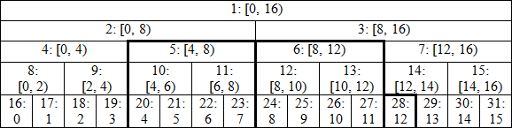
\includegraphics[width=12cm]{lastlazy.png}% Joonise suurus, joonise fail
    \caption{Modifikatsioonid lõikude puul}% Graafi struktuur
    \allikas{Efficient and easy segment trees}% Allikas
    \label{graaf}% Selle järgi viidatakse, pärast käsku \caption
    \end{kk}

Me kutsume funktsiooni modify intervalil $[4, 13)$:
\begin{enumerate}
   \item $l = 20$, $r = 29$, kutsume apply($28$);
   \item $l = 10$, $r = 14$, kutsume calc($14$) — esimene tipp paremalpool praegust intervali on eelmise uuendatud tipu vanem;
   \item $l = 5$, $r = 7$, kutsume calc($7$) seejärel apply($5$) and apply($6$);
   \item $l = 3$, $r = 3$, esimene tsükkel on lõppenud.
\end{enumerate}

Nüüd on võibolla arusaadavam miks on vaja teha - -$l$, põhjusel, et me peame ikkagi arvutama uued väärtused tippudes $2$, $3$ ja $1$.
Lõpetame kui $r > 0$ sest on võimalik, et $l = 1$, $r = 1$ peale esimest tsüklit, ehk peame uuendame juurtippu, aga - -$l$ tulemusena $l = 0$.

Võrreldes eelmise implementatsiooniga, me väldime üleliigseid funktsioonide kutsumisi calc($10$), calc($5$) ja calc($1$).




\chapter{Lõikude puu abil ülesannete lahendamine}
Selles peatükis on antud praktilisem ülevaade lõikude puu ja seotud tehnikatega ülesannete lahendamisest võistlusprogrammeerimises.
Esimeses alapeatükis teeb autor selgeks millal on mõistlik kasutada lõikude puu andmestruktuuri, ning määrab ära millal on see üldse võimalik. 
Alapeatükis 2.2. selgitab autor erinevate lõikude puu abil lahendatavate ülesannete lahenduskäiku. Alapeatükis 2.3. jagab autor enda kogemuse põhjal nõuandeid võistlusel parema tulemuse saavutamiseks. Alapeatükis 2.4. kirjeldab autor kahe informaatikaolümpiaadile omase struktuuriga ülesande koostamise protsessi.
\section{Millistes ülesannetes on mõistlik kasutada lõikude puud?} 
Lõikude puu on andmestruktuur mida saab kasutada monoididega $(S, \cdot: S \times S \to S, e \in S)$, s.o, algebraline struktuur, mis täidab järgmisi omadusi:
\begin{itemize}
    \item assotsiatiivsus: $(a \cdot b) \cdot c$ = $a \cdot (b \cdot c)$ iga $a, b, c \in S$ kohta.
    \item leidub ühikelement: $a \cdot e$ = $e \cdot a$ = $a$ iga $a \in S$ kohta.
\end{itemize}

Sellepärast, et soovime võimaldada kahte sorti päringuid, peame arvestama mis sorti operatsiooni teeme rohkem. Näiteks, kui üks päringutüüp on haruldane, optimiseeriksime ainult teist päringutüüpi, seda on suhteliselt lihtne teha:

\begin{itemize}
    \item Kui me hooliksime ainult massiivi uuendamisoperatsiooni ajakeerukusest, kasutaksime tavapärast massiivi, mis toetab random access massiivi.
    \item Kui tähtis oleks ainult summa leidmise kiirus mingil lõigil kasutaksime prefiksi summa võtet, sest see toetaks selle operatsiooni täitmist ajakeerukusega O(1).
\end{itemize}

Mõlemal korral teeme ühte operatsiooni ajakeerukusega $O(1)$, aga teist operatsiooni $O(n)$ ajakeerukusega. Juhul kui teeme mõlemaid operatsioone umbes sama palju saame teha me kompromissi. Lõikude puud võimaldavad teha täpselt seda, võimaldades $O(\log n)$ ajakeerukust mõlema päringu korral.

\parencite{AC}

On olukordi, kus lõikude puu kasutamine on ainus võimalus ülesannet lahendada, kuigi enamus juhtudel kui väga tahta saab ka ilma.
Näiteks summapäringute korral saab kasutada ka naiivset lähenemist tavalise massiiviga(näiteks  std::vector/std::array), või kasutada lõikude puust lihtsamat võtet nimega prefiksi summa(inglise keeles prefix sum/partial sum).

Järgnevas tabelis on välja toodud erinevad meetodid millega asendada lõikude puud ja nende mitmel tasandil.
\begin{table}[H]
\caption{Lõikude puu asendamine}% Pealkiri
\label{tabel1}% Tabelile viitamine
\scalebox{0.75}{
\begin{tabular}
{r|r|r|r|r|r}% r - paremjoondatud tulp, | - püstjoon
\hline% Horisontaalne joon
Operatsiooni tüüp & Lõikude puu & Massiiv & Prefiksi summa & Hõre tabel & Fenwicki puu\\
\hline
Uuendamine & $O(\log N)$ & $O(1)$ & $O(N)$ & $O(N\log N)$ & $O(\log N)$\\
Summapäring & $O(\log N)$ & $O(N)$ & $O(1)$ & $O(\log N)$ & $O(\log N)$\\
Min/Max leidmine & $O(\log N)$ & $O(N)$ & X & $O(1)$ & $O(\log N)$\\
Implementatsiooni lihtsus & Raske & Lihtne & Lihtne & Keskmine & Raske\\
Implementatsiooni pikkus & Pikk & Lühike & Lühike & Keskmine & Keskmine\\
Intuitiivne & Jah & Jah & Jah & Ei & Ei\\
Selle abil lahendatavaid ülesandeid & Palju & Palju & Vähe & Vähe & Keskmiselt\\
Ruumikeerukus & $O(N)$ & $O(N)$ & $O(N)$ & $O(N\log N)$ & $O(N)$\\
\hline
\end{tabular}
}
\allikas{Autori kogutud andmed}% Viide
\end{table}


Nagu tabelist on näha, on lõikude puu suurimateks eelisteks suur selle abil lahendatavate ülesannete hulk, intuitiivsus ja samaaeg hea keskmine ajakeerukus(muidu kasutaksime lihtsalt massiivi).

Tihti leidub ka lihtsaimaid andmestruktuure standardteegis, nagu nt unordered\_set(C++), millele on omane ajakeerukus $O(1)$, väga paljude operatsioonide korral(kuigi nende operatsioonide konstant on suhteliselt suur). 
Nende implementeerimise lihtsuse tõttu, on tihti mõistlik kasutada hoopis standardteegi andmestruktuure, aga võistlusprogrammeerimisülesannete keerukus seisnebki tihti selles et peab looma oma andmestruktuuri, ning ülesannete loojad soovivadki teha selle vajalikuks(selle jaoks uurivad, mis andmestruktuurid on praegu saadval, nt C++ STL-s).

Siia on lisatud ka tabel, mis on täpsemalt orienteeritud Fenwicki puu ja lõikude puu erinevustele:
\begin{table}[H]
\caption{Lõikude puu ja Fenwicki puu võrdlus, autori tõlgitud}
\begin{tabular}{|l|l|l|}
\hline
Omadus/Funktsioon                         & Fenwicki puu    & Lõikude puu     \\ \hline
Massiivist puu ehitamine                  & $O(n+m)$        & $O(n)$          \\ \hline
Muutumatus massiivis lõigu summa leidmine & Saab lihtsamalt & Saab lihtsamalt \\ \hline
Muutuvas massiivis min/max leidmine       & Limiteeritud    & Jah             \\ \hline
Muutuvas massiivis lõigu summa leidmine   & Jah             & Jah             \\ \hline
Lõigu väärtuse leidmise ajakeerukus       & $O(\log m)$     & $O(\log n)$     \\ \hline
Elemendi uuendamise ajakeerukus           & $O(\log m)$     & $O(\log n)$     \\ \hline
Lõigu väärtuse uuendamise ajakeerukus     & $O(\log m)$     & $O(\log n)$     \\ \hline
Standardse implementatsiooni pikkus       & Palju lühem     & Palju pikem     \\ \hline
Modifitseeritud implementatsiooni pikkus  & Pikk            & Pikk            \\ \hline
\end{tabular}  
\allikas{CP Algorithms 4}
\end{table}


Järgnevates tabelites on märgitud võimalikud $N$-i suurused mingi ajakeerukuse ja standardse ülesande ajalimiidi korral\parencite{timecomplexity}. 


\begin{table}[H]% [] sisse märgitakse paigutus H
   \caption{Ajakeerukuste tabel 1, autori tõlgitud}% Allkiri
    \begin{tabular}{|l|l|}
\hline
$n$                & Sobilikud ajakeerukused        \\ \hline
$n\le 10$          & $O(n!), O(n^7), O(n^6)$        \\ \hline
$n\le 20$          & $O(2^n\cdot n), O(n^5)$        \\ \hline
$n\le 80$          & $O(n^4)$                       \\ \hline
$n\le 400$         & $O(n^3)$                       \\ \hline
$n\le 7500$        & $O(n^2)$                       \\ \hline
$n\le 7\cdot 10^4$ & $O(n\sqrt{n})$                 \\ \hline
$n\le 5\cdot 10^5$ & $O(n\log n)$                   \\ \hline
$n\le 5\cdot 10^6$ & $O(n)$                         \\ \hline
$n\le 10^{18}$       & $O(\log ^2n), O(\log n), O(1)$ \\ \hline
\end{tabular}
    \allikas{USACO Guide}% Allikas
    \label{timecomplexity}% Selle järgi viidatakse, pärast käsku \caption viitamine tabeliga
\end{table}


\begin{table}[H]% [] sisse märgitakse paigutus H
   \caption{Ajakeerukuste tabel 2, autori tõlgitud}% Allkiri
    \begin{tabular}{|l|l|l|}
\hline
$n$               & Suurim sobilik ajakeerukus & Näited                                          \\ \hline
$\le [10..11]$    & $O(n!), O(n^6)$            & Permutatsioonide arvutamine                     \\ \hline
$\le [15..18]$    & $O(2^n\cdot n^2)$          & Rändkaupmehe DP                                 \\ \hline
$\le [18..22]$    & $O(2^n\cdot n)$            & Bitimaski DP                                    \\ \hline
$\le 100$         & $O(n^4)$                   & DP kolme dimensiooniga                          \\ \hline
$\le 400$         & $O(n^3)$                   & Floyd Warshalli algoritm                        \\ \hline
$\le 2\cdot 10^3$ & $O(n^2\log _2 n)$          & 2D tsükkel+mingi puu andmestruktuur             \\ \hline
$\le 10^4$        & $O(n^2)$                   & Erinevad sorteerimisalgoritmid                  \\ \hline
$\le 10^6$        & $O(n\log _2 n)$            & Mestimissortimine, lõikude puu ehitamine        \\ \hline
$\le 10^8$        & $O(n), O(\log _2 n), O(1)$ & Esineb harva, kuid siis tasub I/O optimeerida \\ \hline
\end{tabular}
    \allikas{CP Algorithms 3}% Allikas
    \label{idk}% Selle järgi viidatakse, pärast käsku \caption viitamine tabeliga
\end{table}


Tabel on ehitatud üles ka teadmisele, et keskmiselt suudavad võistlusprogrammeerimisele omased hindamis-serverid teha $10^8$ operatsiooni sekundis. Algoritmi tegelik kiirus ei kuigi pea täpselt vastama tabelis märgitud relevantsele ajakeerukesele, vaid võib ka olla kiirem või aeglasem.

Määrata kas ülesandes nõutakse lõikude puud või mitte, saab näiteks, esmalt uurides kas üldse on vaja kasutada mingit lõikude puu poolt võimaldatud võtet, seejärel leides võrdlus-tabelist(või internetist) selle operatsiooni ajakeerukuse, ning viimasena vaadates ajakeerukuset tabelist(ja ülesandest), kas ajakeerukus sobib ülesandes antud $N$-i suuruse korral.

\begin{extra}
Kui ajalimiit ülesandel on piisavalt leebe, siis tasub muidugi proovida ka lühemat, arusaadavamat või lahendajale lihtsamat algoritmi.
\end{extra}
\begin{extra}
Vahepeal saab pragmade(arvutile antud juhised, et arvuti saaks optimiseerida koodi, (vt Lisa 7)) abil suruda ka läbi teoorias liiga aeglase lahenduse, eriti, kui tegu on naiivse või ettearvatava lahendusega, mida on kompilaatoril lihtne optimeerida.
\end{extra}

\section{Ülesannete lahendused ja selgitused} 
Selles peatükis selgitab autor mitmete lõikude puuga lahendatavate ülesannete mõttekäiku, lisatud on ka implementatsioonid, vajadusel joonised.
Ülesanded on jaotatud temaatika järgi, ning iga ülesande juurde on märgitud ka raskusaste skaalal 1-5 tärni(*).
Autor on implementatsioonid üldjuhul kirjutanud iteratiivselt.
Ülesanded on leitavad platvormidel CSES, Codeforces, AtCoder ja nii edasi, ning autor on lisanud iga ülesande juurde\textit{ hyperlingid} veebilehele, kus saab neid esitada.
Olümpiaaditüüpi ülesandeid leidub veel platvormidel nagu näiteks, oj.uz, Kattis, ning ka erinevates CMS judge'i \textit{fork'ides}.
\begin{extra}
Mälulimiite ja ajalimiite mainitakse, ainult juhul kui need on ebastandardsed -- ehk ei ole vastavalt 512 megabaiti ja 1 sekund.
\end{extra}
\subsection{Standardsed ülesanded}
Esimeses alapeatükis on toodud välja erinevaid standardseid ülesandeid koos autori poolt kirjutatud lahendustega.
\begin{prereq}
Lõikude puu(peatükid 1.1-1.5)
\end{prereq}
Standardsed on ülesanded seepärast, et need testivad otseseid teadmisi töö esimesest peatükist, ning ei nõua laiamahulist algoritmide/andmestruktuuride modifitseerimist, ega ka uute ideede tuletamist.
\subsubsection{Dynamic Range Minimum Queries, CSES, *} 
\begin{extra}
Ülesannet saab esitada \href{https://cses.fi/problemset/task/1649}{CSES platvormil}.
\end{extra}
\begin{prereq}
Lõikude puul miinimumi leidmine
\end{prereq}
\begin{Text}
Ülesandes antakse sisendiks $n$ täisarvu, ja peame tegema $q$($1\le n,q\le 2\cdot10^9$) operatsiooni kujul: 
\begin{enumerate}
    \item Uuenda väärtus positsioonil $k$($1\le k\le n$) $u$-ks($1\le x_i,u\le 10^9$).
    \item Tagasta minimaalne väärtus lõigul $[a...b]$($1\le a\le b\le n$).
\end{enumerate}

\parencite{min}
\end{Text}
\begin{Input}
 Esimesel real on kaks täisarvu $n$ ja $q$: massiivi suurus ja päringute arv.

 Teisel real on $n$ täisarvu $x_1,x_2,...,x_n$: massiivi elementide väärtused.

 Seejärel, antakse $q$ rida päringuid: igaüks kujul $1$ $k$ $u$ või $2$ $a$ $b$.
\end{Input}

\begin{Output}
Väljasta vastus igat teist tüüpi päringule.
\end{Output}

\textbf{Näidissisend
}
\begin{verbatim}
8 4
3 2 4 5 1 1 5 3
2 1 4
2 5 6
1 2 3
2 1 4
\end{verbatim}

\textbf{Näidisväljund}

\begin{verbatim}
2
1
3
\end{verbatim}



\begin{vihje}
$min()$ on kommutatiivne ehk lihtsalt kasuta tavapärast lõikude puud lõigul miinimumi leidmiseks.
\end{vihje}
\begin{solution}
Selgitus on leitav peatükis maksimumi ja miinimumi leidmine lõigus, ja peatüki iteratiivne implementatsioon alapeatükis lõigul summa leidmine.
\end{solution}

\begin{cclol}
#include <bits/stdc++.h>

using namespace std;

#pragma GCC optimize("O3,unroll-loops")
#pragma GCC target("avx2,bmi,bmi2,popcnt,lzcnt")

const int MA = 2e5;
int n;
int t[2 * MA];

void build() {
for (int i = n - 1; i > 0; --i) t[i] = min(t[i << 1], t[i << 1 | 1]);
}

void modify(int p, int value) {
for (t[p += n] = value; p > 1; p >>= 1) t[p >> 1]=min(t[p], t[p ^ 1]);
}

int query(int l, int r) {
  int res = INT_MAX;
  for (l += n, r += n; l < r; l >>= 1, r >>= 1) {
    if (l & 1) res = min(res, t[l++]);
    if (r & 1) res = min(res, t[--r]);
  }
  return res;
}

int main(int argc, char ** argv) {
  ios_base::sync_with_stdio(false);
  cin.tie(NULL);
  int q;
  cin >> n >> q;
  for (int i = 0; i < n; ++i) cin >> t[i + n];

  build();

  int g, c, d;
  for (int i = 0; i < q; i++) {
    cin >> g >> c >> d;

    if (g == 1) modify(c - 1, d);
    else if (g == 2) cout << query(c - 1, d) << endl;
    else if (g == 2 && c == d) cout << t[c - 1 + n] << endl;
  }

  return 0;
}
\end{cclol}
 \begin{kk}[H]% [] sisse märgitakse paigutus H
    \caption{Lahendus   ülesandele Dynamic Range Minimum Queries}% Allkiri
    \allikas{Autori kirjutatud kood}% Allikas
    \label{mkm}% Selle järgi viidatakse, pärast käsku \caption
    \end{kk}

Programmi ajakeerukus on $O(N\log N)$.
\begin{extra}
Ei tohi unustada, et kasutatakse intervallinotatsiooni(s.t $[)$) ja ka $0$-põhist indekseerimist, ning tihti summade leidmisel on vaja kasutada suuremahulisi andmetüüpe nagu nt $long\ long$(Lisa 4).
\end{extra}
\begin{extra}
CSES süsteemis on avatud testid.
\end{extra}

\subsubsection{Segment tree for the minimum, Codeforces EDU, *}
\begin{extra}
Ülesannet saab esitada \href{https://codeforces.com/edu/course/2/lesson/4/1/practice/contest/273169/problem/B}{Codeforces platvormi EDU kursuste lehel}.
\end{extra}
\begin{prereq}
Lõikude puul miinimumi leidmine
\end{prereq}
\begin{extra}
See ülesanne on peaaegu identne eelmisega.
\end{extra}
\begin{Text}
Leia miinimum antud lõigul.

\parencite{semin}
\end{Text}

\begin{Input}
Algselt antakse sisendiks kaks täisarvu $n$ ja $m$ ($1\le n,m\le 1000001\le n,m\le 100000$), mis on vastavalt massiivi suurus ja päringute arv.
Järgmisena antakse siendiks $n$ numbrit $a
_i$, mis tähistavad massiivi algseid väärtusi($0\le a_i\le 10^9,0\le a_i\le 10^9$).
Järgmised $m$ rida sisaldavad operatsioonide kirjeldusi kujul:
\begin{enumerate}
\item $1$ $i$ $v$: muuda elemendi, mille indeks on $i$, $v$ väärtuseks ($0\le i<n, 0\le i<n$, $0\le v\le 10^9, 0\le v\le 10^9$).
\item $2$ $l$ $r$: leia miinimum loigus $l$...$r−1$($0\le l<r\le n$, $0\le l<r\le n$).
\end{enumerate}
\end{Input}
\begin{Output}
Väljasta iga teist tüüpi päringu vastus.
\end{Output}

\textbf{Näidissisend}

\begin{verbatim}
5 5
5 4 2 3 5
2 0 3
1 2 6
2 0 3
1 3 1
2 0 5
\end{verbatim}

\textbf{Näidisväljund}

\begin{verbatim}
2
4
1
\end{verbatim}



\begin{vihje}
$min()$ on kommutatiivne operatsioon ehk lihtsalt kasuta tavapärast lõikude puud lõigul miinimumi leidmiseks.
\end{vihje}

\begin{solution}
Selgitus on leitav peatükis maksimumi ja miinimumi leidmine lõigus, ja peatüki iteratiivne implementatsioon alapeatükis lõigul summa leidmine.
\end{solution}

\begin{cclol}
#include <bits/stdc++.h>

using namespace std;

#define ll long long
#define cint
const int

#pragma GCC optimize("O3,unroll-loops")
#pragma GCC target("avx2,bmi,bmi2,popcnt,lzcnt")

cint MM = 1e9 + 7;
cint MA = 2e5 + 5;

ll t[2 * MA];
int n;

void build() {
  for (int i = n - 1; i > 0; i--) {
    t[i] = min(t[i << 1], t[i << 1 | 1]);
  }
}

void modify(int x, int val) {
for (t[x += n] = val; x > 1; x >>= 1) t[x >> 1]=min(t[x], t[x ^ 1]);
}

ll sum(int l, int r) {
  ll smol = MM;
  for (l += n, r += n; l < r; l >>= 1, r >>= 1) {
    if (l & 1) smol = min(smol, t[l++]);
    if (r & 1) smol = min(smol, t[--r]);
  }
  return smol;
}

int main(int argc, char ** argv) {
  ios_base::sync_with_stdio(false);
  cin.tie(NULL);
  int m;
  cin >> n >> m;
  for (int i = 0; i < n; i++) {
    cin >> t[i + n];
  }
  build();
  for (int i = 0; i < m; i++) {
    int type;
    cin >> type;
    if (type == 1) {
      int x, v;
      cin >> x >> v;
      modify(x, v);
    } else {
      int l, r;
      cin >> l >> r;

      cout << sum(l, r) << endl;
    }
  }

  return 0;
}
    \end{cclol}
    \begin{kk}[H]
    \caption{Lahendus ülesandele Segment tree for the minimum}% Allkiri
    \allikas{Autori implementatsioon}% Allikas
    \end{kk}
    
Ajakeerukus on $O(N\log N)$.

\begin{extra}%useful notice
Codeforces EDU ei võimalda avatud teste, ning läbi lähevad tihti ka suboptimaalsed lahendused.
\end{extra}

\subsubsection{Dynamic Range Sum Queries, CSES, *}
\begin{extra}
Ülesannet saab esitada \href{https://cses.fi/problemset/task/1648}{CSES platvormil}.
\end{extra}
\begin{prereq}
Lõikude puul summa leidmine
\end{prereq}
\begin{Text}
Tuleb vastata $q$ päringule kujul:
\begin{enumerate}
\item Võttes sisendiks indeksi $k$ ja väärtuse $x$, määrata $k$-ndale elemendile väärtus $x$.
\item Kui on antud kaks indeksit $a$ ja $b$, leidke vahemiku $[a,b]$ elementide summa.
\end{enumerate}

$(1\le n,q\le 2\cdot 10^5)$

\parencite{sum}
\end{Text}

\begin{Input}
Esimesel real on kaks täisarvu $n$ ja $q$$(1\le n,q\le 2\cdot 10^5)$: massiivi suurus ja päringute arv.

Teisel real on antud $n$ täisarvu $x_1,x_2,...,x_n$$(1\le x_i,u\le 10^9)$: massiivi elementide väärtused.

Seejärel antakse $q$ päringut kujul $1$ $k$ $u$$(1\le k\le n)$ või $2\ a\ b$$(1\le a\le b\le n)$.
\end{Input}
\begin{Output}
Väljasta iga teist tüüpi päringu vastus.
\end{Output}

\textbf{Näidissisend}

\begin{verbatim}
8 4
3 2 4 5 1 1 5 3
2 1 4
2 5 6
1 3 1
2 1 4
\end{verbatim}

\textbf{Näidisväljund}

\begin{verbatim}
14
2
11
\end{verbatim}


\begin{vihje}
Ainus erinevus eelmise ülesandega võrreldes on see, et vajalikuks operatsiooniks on miinimumi leidmise asemel summa arvutamine.
\end{vihje}

\begin{vihje}
Kasute long long andmetüüpi.
\end{vihje}

\begin{cclol}
#include <bits/stdc++.h>

using namespace std;

#pragma GCC optimize("O3,unroll-loops")
#pragma GCC target("avx2,bmi,bmi2,popcnt,lzcnt")

const int N = 2e5;
int n;
long long t[2 * N];

void build() {
  for (int i = n - 1; i > 0; --i) t[i] = t[i << 1] + t[i << 1 | 1];
}

void modify(int p, int value) {
  for (t[p += n] = value; p > 1; p >>= 1) t[p >> 1] = t[p] + t[p ^ 1];
}

long long query(int l, int r) {
  long long res = 0;
  for (l += n, r += n; l < r; l >>= 1, r >>= 1) {
    if (l & 1) res += t[l++];
    if (r & 1) res += t[--r];
  }
  return res;
}

int main(int argc, char ** argv) {
  int q;
  cin >> n >> q;
  for (int i = 0; i < n; ++i) cin >> t[i + n];

  build();

  int g, c, d;
  for (int i = 0; i < q; i++) {
    cin >> g >> c >> d;

    if (g == 1) modify(c - 1, d);
    else if (g == 2) cout << query(c - 1, d) << endl;
  }

  return 0;
}
\end{cclol}
 \begin{kk}[H]% [] sisse märgitakse paigutus H
    \caption{Ülesande Dynamic Range Sum Queries lahendus}% Allkiri
    \allikas{Autori implementatsioon}% Allikas
    \label{mkm}% Selle järgi viidatakse, pärast käsku \caption
    \end{kk}

Ajakeerukus on $O(N\log N)$.

\subsubsection{Range Update Queries, CSES, **}
\begin{extra}
Ülesannet saab esitada \href{https://cses.fi/problemset/task/1651}{CSES platvormil}.
\end{extra}
\begin{prereq}
Lõikude puul ühe elemendi väärtuse leidmine(+ nn mass-change operations)
\end{prereq}

\begin{Text}
Pead täitma massiivil suurusega $n$ kahte liiki $q$ päringuid kujul:
\begin{enumerate}
\item Iga elemendi väärtuse suurendamine vahemikus $a...b$ $u$ võrra.
\item Väärtuse leidmine positsioonil indeksiga $k$.
\end{enumerate}

\parencite{update}
\end{Text}

\begin{Input}
Esimesel real on antud kaks täisarvu $n$ ja $q$: massiivi suurus ja päringute arv.

Teisel real on antud $n$ elementi $x_1,x_2,...,x_n$.

Seejärel on antud $q$ päringut kujul $1\ a\ b\ u$ või $2\ k$.
\end{Input}
\begin{Output}
Väljasta iga teist tüüpi päringu vastus.
\end{Output}

\textbf{Näidissisend}

\begin{verbatim}
8 3
3 2 4 5 1 1 5 3
2 4
1 2 5 1
2 4
\end{verbatim}

\textbf{Näidisväljund}

\begin{verbatim}
5
6
\end{verbatim}


\begin{vihje}
Lihtsalt modifitseeri standardseid implementatsioone, tegu on ikkagi kommutatiivsete operatsioonidega.
\end{vihje}

\begin{solution}
Ülesande implementatsioon ühtib implementatsiooniga leheküljel 34.
\end{solution}


\begin{cclol}
#include <bits/stdc++.h>

using namespace std;

#define cint
const int

#pragma GCC optimize("O3,unroll-loops")
#pragma GCC target("avx2,bmi,bmi2,popcnt,lzcnt")

cll ML = 1e18;
cint MN = 1e9;
cint MA = 2e5 + 10;
cint MM = 1e9 + 7;

vector < ll > t(2 * MA, 0);
int n;

void build() {
  for (int i = 0; i > 0; i--) t[i] = t[i << 1] + t[i << 1 | 1];
}

ll pointVal(int x) {
  ll res = 0;
  for (x += n; x > 0; x >>= 1) res += t[x];
  return res;
}

void add(int l, int r, int val) {
  for (l += n, r += n; l < r; l >>= 1, r >>= 1) {
    if (l & 1) t[l++] += val;
    if (r & 1) t[--r] += val;
  }
}

int main(int argc, char ** argv) {
  ios_base::sync_with_stdio(false);
  cin.tie(NULL);
  int m;
  cin >> n >> m;
  for (int i = 0; i < n; i++) {
    cin >> t[i + n];
  }
  build();
  for (int i = 0; i < m; i++) {
    int type;
    cin >> type;
    if (type == 1) {
      int l, r, val;
      cin >> l >> r >> val;
      l--;
      add(l, r, val);
    } else if (type == 2) {
      int x;
      cin >> x;
      x--;
      cout << pointVal(x) << endl;
    }
  }
  return 0;
}
    \end{cclol}
    \begin{kk}[H]
    \caption{CSES Range Update Queries}% Allkiri
    \allikas{Autori implementatsioon}% Allikas
    \end{kk}

Ajakeerukus on $O(N\log N)$.


\begin{extra}
See on viimane siin töös käsitletud standardne ülesanne, kui arvad, et vajad rohkem harjutamist sobib selleks kas Codeforces EDU esimene peatükk või range queries peatükk CSES Problemset'is. 
Kuid teoorias peaks nendest teadmistest piisama, et lahendada peaaegu kõiki lõikude puu ülesandeid, peale nende mis nõuavad laiska laienemist.
\end{extra}


    
\subsection{Raskemad ülesanded}
Siin peatükis on sedasorti ülesanded mis nõuavad natuke rohkem mõtisklemist, ning mis ei ole lahendatavad lihtsalt standardse implementatsiooni ümber kirjutamisega.
Selles peatükis on üldjuhul selgitused ka pikemad sest lahendused nõuavad pikemat mõttekäiku.
\begin{prereq}
Lõikude puu(peatükid 1.1-1.6)
\end{prereq}
\subsubsection{Number of minimums on a segment, Codeforces EDU, **}
\begin{extra}
Ülesannet saab esitada \href{https://codeforces.com/edu/course/2/lesson/4/1/practice/contest/273169/problem/C}{Codeforces platvormi EDU kursuste lehel}.
\end{extra}
\begin{prereq}
Lõigul miinimumi leidmine lõikude puu abil
\end{prereq}
\begin{Text}
Leia antud lõigul mitme elemendi väärtus on võrdne minimaalse elemendi väärtusega lõigul.

\parencite{minseg}
\end{Text}
\begin{Input}
Algselt antakse sisendiks kaks arvu $n$ ja $m$, kus $(1\le n,m\le 10^5)$, mis tähistavad massiivi suurust ja päringute arvu.
Järgneb $n$ elementi, massiivi $a[]$ elementide väärtused $a_i$$(0\le a_i\le 10^9)$.
Järgmisel real antakse $q$ päringut kujul:
\begin{enumerate}
\item $1$ $i$ $v$: muuda elemendi indeksiga $i$ väärtus võrdseks $v$ väärtusega$(0\le i<n, 0\le v\le 10^9)$.
\item $2$ $l$ $r$: leia elementide arv lõigus l...r−1, mis on võrdne $min(a_l...a_{r-1})$ väärtusega$(0\le l<r\le n)$.
\end{enumerate}

\end{Input}
\begin{Output}
Iga teist tüüpi päringu kohta väljasta kaks täisarvu: miinimum lõigul ja mitu elementi on võrdsed miinimumi väärtusega lõigul.
\end{Output}

\textbf{Näidissisend}

\begin{verbatim}
5 5
3 4 3 5 2
2 0 3
1 1 2
2 0 3
1 0 2
2 0 5
\end{verbatim}

\textbf{Näidisväljund}

\begin{verbatim}
3 2
2 1
2 3
\end{verbatim}



\begin{vihje}
Ülesande keeruliseimaks osaks on implementeerimine.
\end{vihje}

\begin{vihje}
Kasuta pair'e.
\end{vihje}

\begin{solution}
Peame salvestama igal lõigul kahte sorti andmeid, kasutades pair'e:
\begin{itemize}
\item Milline on minimaalne väärtus lõigul, ütleme et see on $min$.
\item Mitu elementi lõigul on võrdsed minimaalse väärtusega lõigul, utleme et see on $cnt$.
\end{itemize}

Kuidas arvutada väärtused?

Ütleme, et meil on ($m_1$, $c_1$) ja ($m_2$, $c_2$), ehk mõlema lõigu kohta $min$ ja $cnt$:
\begin{itemize}
\item Kui $m_1<m_2$, siis miinimum on $m_1$, ja sellega võrdsete elementide arv on $c_1$, siis kombineerides saame $m_1$, $c_1$. 
\item Sarnaselt, kui $m_1>m_2$, siis saame $(m_2,c_2)$. 
\item Kui $m1=m2$, siis miinimumid on võrdsed. Saame miinimumide arvuks uuel lõigul $c_1+c_2$, saame pair($m_1$, $c_1+c_2$).
\end{itemize}
\end{solution}

Idee on üsna lihtne põhjusel, et mõlemad operatsioonid on kommutatiivsed, implementatsioon võib kuigi muutuda natuke tüütuks:
\begin{cclol}
#include <bits/stdc++.h>

using namespace std;

#define cint
const int
#define pii pair < int, int >

#pragma GCC optimize("O3,unroll-loops")
#pragma GCC target("avx2,bmi,bmi2,popcnt,lzcnt")

cint MA = 2e5 + 10;

vector < pair < int, int >> t(MA, pair < int, int > {});
int n;

void build() {
  for (int i = n - 1; i > 0; i--) {
    t[i].first = min(t[i << 1].first, t[i << 1 | 1].first);
    if (t[i << 1].first < t[i << 1 | 1].first) {
      t[i].second = t[i << 1].second;
    } else if (t[i << 1].first > t[i << 1 | 1].first) {
      t[i].second = t[i << 1 | 1].second;
    } else {
      t[i].second = t[i << 1].second + t[i << 1 | 1].second;
    }
  }
}

void modify(int x, int val) {
  for (t[x += n].first = val; x > 1; x >>= 1) {
    t[x >> 1].first = min(t[x].first, t[x ^ 1].first);
    if (t[x].first < t[x ^ 1].first) {
      t[x >> 1].second = t[x].second;
    } else if (t[x].first > t[x ^ 1].first) {
      t[x >> 1].second = t[x ^ 1].second;
    } else {
      t[x >> 1].second = t[x].second + t[x ^ 1].second;
    }
  }
}

pair < int, int > mn(int l, int r) {
  pii pp = {
    MM,
    0
  };
  for (l += n, r += n; l < r; l >>= 1, r >>= 1) {
    if (l & 1) {
    if (t[l].first < pp.first) pp.second = t[l].second;
    else if (t[l].first == pp.first) pp.second += t[l].second;
    pp.first = min(pp.first, t[l++].first);
    }
    if (r & 1) {
    if (t[r - 1].first < pp.first) pp.second = t[r - 1].second;
    else if (t[r - 1].first == pp.first) pp.second += t[r - 1].second;
    pp.first = min(pp.first, t[--r].first);
    }
  }
  return pp;
}

int main(int argc, char ** argv) {
  ios_base::sync_with_stdio(false);
  cin.tie(NULL);
  int m;
  cin >> n >> m;
  for (int i = 0; i < n; i++) {
    cin >> t[i + n].first;
    t[i + n].second = 1;
  }
  build();
  for (int i = 0; i < m; i++) {
    int type;
    cin >> type;
    if (type == 1) {
      int x, v;
      cin >> x >> v;
      modify(x, v);
    } else {
      int l, r;
      cin >> l >> r;

      pii ans = mn(l, r);
      cout << ans.first << " " << ans.second << endl;
    }
  }

  return 0;
}
    \end{cclol}
    \begin{kk}[H]
    \caption{Lahendus ülesandele Number of minimums on a segment}% Allkiri
    \allikas{Autori implementatsioon}% Allikas
    \end{kk}

Ajakeerukus on $O(N\log N)$.


\subsubsection{Applying max to segment, Codeforces EDU, **}
\begin{extra}
Ülesannet saab esitada \href{https://codeforces.com/edu/course/2/lesson/5/1/practice/contest/279634/problem/B}{Codeforces platvormi EDU kursuste lehel}.
\end{extra}
\begin{prereq}
Lõikude puu abil lõigul miinimumi ja maksimumi leidmine
\end{prereq}

\begin{Text}
Antud on massiiv $n$ elemendiga, kus algselt on iga elemendi väärtus võrdne nulliga.

Pead täitma kahte sorti päringuid:
\begin{enumerate}
\item iga $i$ kohta lõigul $l...r-1$ tee operatsioon $a_i=max(a_i, v)$, kus $v$ on antud.
\item leia indeksiga $i$ elemendi väärtus.
\end{enumerate}

\parencite{inseg}
\end{Text}
\begin{Input}
Algselt antakse sisendiks kaks arvu $n$ ja $m$, massiivi suurus ja päringute arv $(1\le n,m\le 10^5)$.
Sellel järgneb $m$ operatsiooni kujul:
\begin{itemize}
\item $1\ l\ r\ v$: iga $i$ kohta lõigul $l..r-1$ tee operatsioon $a_i=max(a_i,v)$$(0\le l<r\le n; 0\le v\le 10^9)$,
\item $2\ i$: leia indeksiga $i$$(0\le i<n)$ elemendi väärtus.
\end{itemize}

\end{Input}
\begin{Output}
Väljasta iga teist tüüpi päringu vastus.
\end{Output}

\textbf{Näidissisend}

\begin{verbatim}
5 5
1 0 3 3
2 1
1 2 4 4
2 3
2 4
\end{verbatim}

\textbf{Näidisväljund}

\begin{verbatim}
3
4
0
\end{verbatim}


\begin{vihje}
Ülesande lahendus on sarnane varem tutvustatud ülesande Range Update Queries lahendusele, lihtsalt asendame look funktsioonis liitmise maksimumi leidmisega, see töötab põhjusel, et max on samuti kommutatiivne operatsioon.
\end{vihje}

\begin{cclol}
#include <bits/stdc++.h>

using namespace std;

#pragma GCC optimize("O3,unroll-loops")
#pragma GCC target("avx2,bmi,bmi2,popcnt,lzcnt")

vector < int > t(2 * MA, 0);
int n;

void mx(int l, int r, int val) {
  for (l += n, r += n; l < r; l >>= 1, r >>= 1) {
    if (l & 1) {
      t[l] = max(t[l], val);
      l++;
    }
    if (r & 1) {
      r--;
      t[r] = max(t[r], val);
    }
  }
}

int look(int x) {
  int res = 0;
  for (x += n; x > 0; x >>= 1) res = max(res, t[x]);
  return res;
}

int main() {
  ios_base::sync_with_stdio(false);
  cin.tie(NULL);
  int m;
  cin >> n >> m;
  for (int i = 0; i < m; i++) {
    int type;
    cin >> type;
    if (type == 1) {
      int l, r, val;
      cin >> l >> r >> val;
      mx(l, r, val);
    } else {
      int x;
      cin >> x;
      cout << look(x) << endl;
    }
  }

  return 0;
}
    \end{cclol}
    \begin{kk}[H]
    \caption{Codeforces, Applying MAX on a segment}% Allkiri
    \allikas{Autori implementatsioon}% Allikas
    \end{kk}

Ajakeerukus on $O(N\log N)$.


\subsubsection{K-th one, Codeforces EDU, **}
\begin{extra}
Ülesannet saab esitada \href{https://codeforces.com/edu/course/2/lesson/4/2/practice/contest/273278/problem/B}{Codeforces platvormi EDU lehel}.
\end{extra}
\begin{prereq}
Lõikude puuga $k$-nda elemendi leidmine
\end{prereq}
\begin{Text}
Ülesandes on vaja leida leida massiivis $k$-nda ühe asukoht.

\parencite{14}
\end{Text}

\begin{Input}
Algselt antakse sisendiks kaks täisarvu $n$ ja $m$$(1\le n, m\le 10^5)$: massiivi suurus ja päringute arv.

Järgmisel real on n arvu $a_i$ massiivi $a[]$ algsed väärtused, kus $a_i\in\{0, 1\}$.

Sellele järgneb $m$ päringut kujul:
\begin{itemize}
\item $1$ $i$: muuda elemendi indeksiga $i$ väärtus vastupidiseks, s.t $0\rightarrow 1$ või $1\rightarrow 0$. 
\item $2$ $k$: leia k-ndas $1$(kasutusel on nullipõhine indekseerimine, ning samuti on alati garanteeritud, et massiivis on piisavalt $1$ väärtusega elemente).
\end{itemize}
\end{Input}
\begin{Output}
Iga teist tüüpi päringu kohta väljasta otsitava ühe indeks(alustades loendamist nullist).
\end{Output}

\textbf{Näidissisend}

\begin{verbatim}
5 7
1 1 0 1 0
2 0
2 1
2 2
1 2
2 3
1 0
2 0
\end{verbatim}

\textbf{Näidisväljund}

\begin{verbatim}
0
1
3
3
1
\end{verbatim}


\begin{vihje}
Piisab standardsetest lõikude puu operatsioonidest.
\end{vihje}

\begin{solution}
Peamine idee on järgnev: kasutame summaoperatsiooni võimaldavat lõikude puud. Elemendi väärtusi muudame samuti standardsel viisil. 
$k$-nda ühe leidmine on sarnane vasakpoolseima prefiksi leidmine mille summa on võrdne $k+1$. 

Algoritm ise on üsna lihtne.

Ütleme, et meil on vaja leida k-ndas üks lõigul $[l,r)$:
\begin{itemize}
\item Kui $r=l+1$, siis leidsime soovitud $1$. 
\item Vastasel juhul, me vaatleme summat vasakpoolsel alamlõigul. 
\item Kui $k<s$, siis k-ndas üks on vasakpoolses alampuus. 
\item Teisel juhul, me peame alustama otsingut ühele indeksiga $k−s$ parempoolses alampuus. Nagu teada, on elemendi leidmise ajakeerukus $O(\log n)$. 
\end{itemize}
Näiteks, me ehitame lõikude puu summa operatsiooniga:
\begin{itemize}
\item Teeme $find(3)$. 
\item Me alustame juures, lõigul $[0,8)$, ja otsime kolmandat ühte. 
\item Nüüd vaatame vasakpoolset alamlõiku $[0,4)$ ja saame, et selle summa on $2$, mis on vähem kui $k+1=4$. 
\item Järelikult, liigume alla parempoolsele alamlõigule $[4,8)$ ja otsime $k−2=3−2=1$ -- ühte sellel lõigul.
\item Vasakpoolsel alamlõigul $[4,6)$, on summa $2$, mis on vähem kui või võrdne $k+1=1+1=2$, siis see asub alamlõigus $[4,6)$.
\item Lõpuks, vasakpoolsel alamlõigul $[4,5)$,summa on $1$, mis on samuti vähem kui $2$, see tähendab, et otsitav $1$ on parempoolses alamlõigus.
\end{itemize}

\begin{figure}[H]% [] sisse märgitakse paigutus H
    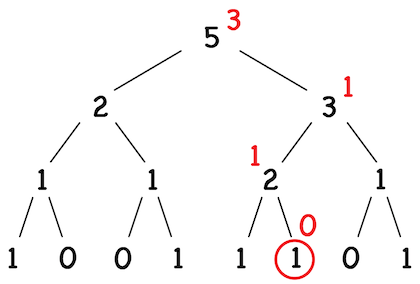
\includegraphics[width=12cm]{kth.png}% Joonise suurus, joonise fail
    \caption{$k$-nda elemendi leidmine}% Allkiri
    \allikas{Codeforces EDU}% Allikas
    \label{joonis}% Selle järgi viidatakse, pärast käsku \caption
\end{figure}
\end{solution}
Järgnev on üks viis kuidas implementeerida seda lahendust:
\begin{cclol}
#include <bits/stdc++.h>

using namespace std;
#define ll long long

ll glb;
void build_tree(ll * a, ll  s, ll e, ll * tree, ll  index) {
  if (s == e) {
    tree[index] = a[s];
    return;
  }
  ll int mid = (s + e) / 2;
  build_tree(a, s, mid, tree, 2 * index);
  build_tree(a, mid + 1, e, tree, 2 * index + 1);
  tree[index] += tree[2 * index] + tree[2 * index + 1];
  return;
}

ll query(ll * tree, ll ss, ll se, ll & k, ll index) {
  if (glb != -1 || tree[index] == 0)
    return INT_MAX;

  if (tree[index] < k) {
    k -= tree[index];
    return INT_MAX;
  }
  if (ss == se) {
    glb = ss;
    return ss;
  }
  ll int mid = (ss + se) / 2;
  ll int left = query(tree, ss, mid, k, 2 * index);
  ll int right = query(tree, mid + 1, se, k, 2 * index + 1);
  return min(left, right);
}
void point_update(ll * tree, ll ss, ll se, ll i, ll inc, ll index) {
  if (i > se || i < ss)
    return;
  if (ss == se) {
    tree[index] = inc;
    return;
  }
  ll int mid = (ss + se) / 2;
  point_update(tree, ss, mid, i, inc, 2 * index);
  point_update(tree, mid + 1, se, i, inc, 2 * index + 1);
  tree[index] = tree[2 * index] + tree[2 * index + 1];
  return;
}
void solve() {
  int n, q;
  cin >> n >> q;

  ll a[n];
  for (int i = 0; i < n; i++)
    cin >> a[i];
  ll tree[4 * n + 1] = {
    0
  };

  build_tree(a, 0, n - 1, tree, 1);

  while (q--) {
    ll num, l;
    cin >> num >> l;
    if (num == 1) {
      point_update(tree, 0, n - 1, l, !a[l], 1);
      a[l] = !a[l];
    } else {
      l++;
      glb = -1;
      ll x = query(tree, 0, n - 1, l, 1);
      cout << x << endl;
    }

  }

}
int main() {
  ios_base::sync_with_stdio(false);
  cin.tie(NULL);

  ll int t = 1;
  while (t--) {
    solve();
  }

  return 0;
}
\end{cclol}
\begin{kk}[H]% [] sisse märgitakse paigutus H
    \caption{Implementatsioon}% Allkiri
    \allikas{Manan Ghetia GitHub}% Allikas
    \label{EMaxx}% Selle järgi viidatakse, pärast käsku \caption
    \end{kk}
\subsubsection{First element at least X, Codeforces EDU, **}
\begin{extra}
Ülesannet saab esitada \href{https://codeforces.com/edu/course/2/lesson/4/2/practice/contest/273278/problem/C}{Codeforces platvormi EDU lehel}.
\end{extra}
\begin{prereq}
Lõikude puu abil esimese elemendi leidmine, mille väärtus on vähemalt $x$.
\end{prereq}
\begin{Text}
Ülesandes on vaja leida minimaalne indeks $j$, kus $a[j]\ge x$.

\parencite{14.1}
\end{Text}

\begin{Input}
Esimesel real on kaks täisarvu $n$ ja $m$$(1\le n,m\le 10^5)$: massiivi suurus ja päringute arv. Järgmisel real on $n$ arvu $a_i$$(0\le a_i\le 10^9)$, massiivi elementide algsed väärtused. 

Sellele järgnevad $m$ rida kahte sorti päringuid:
\begin{itemize}
    \item $1$ $i$ $v$ -- muuda indeksiga $i$ elemendi väärtus võrdseks arvu $v$$(0\le i\le n; 0\le v\le 10^9)$ väärtusega.
    \item $2$ $x$ -- leia minimaalne indeks $j$ kujul, et $a_j\geq x$, kui sellist elementi ei ole väljasta hoopis $-1$, kasutame 0-põhist indekseerimist. 
\end{itemize}
\end{Input}
\begin{Output}
Väljasta iga teist tüüpi päringu vastus.
\end{Output}


\textbf{Näidissisend}

\begin{verbatim}
5 7
1 3 2 4 6
2 2
2 5
1 2 5
2 4
2 8
1 3 7
2 6
\end{verbatim}

\textbf{Näidisväljund}

\begin{verbatim}
1
4
2
-1
3
\end{verbatim}


\begin{vihje}
Lähenemine on sarnane eelmisele ülesandele.
\end{vihje}

\begin{solution}
Algselt teeme sama mis eelmises ülesanded: 
\begin{enumerate}
\item Ehitame lõikude puu, mis toetab $max$ operatsiooni.
\item Selle jaoks, et otsida elementi lõigus, kui seal on $max$ vähemalt väärtusega $x$, liigume alla vasakpoolsele alampuule,teisel juhul, me liigume alla parempoolsele alampuule.
\end{enumerate}


Nüüd selgitame uut ja keerulisemat osa:
\begin{itemize}
\item Peame vastama päringule -- $first\_above(x,l)$: leiame esimese elemendi mis on $l$-st parem pool ning suurem või võrdne $x$-ga.
\item Selle leidmiseks teeme rekursiivselt järgnevat: oletame, et tahame leida lõigul taolist elementi. 
\item Kui maksimaalne vasakpoolsel alamlõigul on väiksem või suurem kui $x$ ja lõik lõikub lõiguga $[l,n)$, seejärel alustame liikumist rekursiivselt vasakust alampuust, kui me ei leia elementi vasakpoolses alamlõigus, siis jätkame parempoolsel alamlõigul. Päring täidetakse siis logaritmilise ajakeerukusega. 
\end{itemize}
Algoritmi ajakeeukus on $O(\log n)$.
\end{solution}

\begin{cclol}
#include <bits/stdc++.h>
using namespace std;
#define ll long long

ll gb=-1;
void build_tree(ll *a, ll s, ll e, ll *tree, ll index)
{
	if(s==e)
	{
		tree[index] = a[s];
		return;
	}
	ll int mid = (s+e)/2;
	build_tree(a,s,mid,tree,2*index);
	build_tree(a,mid+1,e,tree,2*index+1);
	tree[index] = max(tree[2*index],tree[2*index+1]);
	return;
}
void query(ll int *tree,ll int ss,ll int se,ll x ,ll int index)
{
	
	if(tree[index]<x)
	return;
	if(gb>=0)
	return;
	if(ss==se)
	{
		if(tree[index]>=x)
		gb=ss;
		return;
	}
	ll int mid = (ss + se)/2;
	 query(tree,ss,mid,x,2*index);
	 query(tree,mid+1,se,x,2*index+1);
	 return;
}
void point_update(ll *tree,ll ss,ll se,ll i,ll inc,ll index)
{
	if(i>se || i<ss)
	return;
	if(ss == se)
	{
		tree[index] = inc;
		return;
	}
	ll int mid = (ss + se)/2;
	point_update(tree,ss,mid,i,inc,2*index);
	point_update(tree,mid+1,se,i,inc,2*index+1);
	tree[index] = max(tree[2*index],tree[2*index+1]);
	return;
}

void solve()
{
	int n,q;
	cin>>n>>q;
	
	ll a[n];
	for(int i=0;i<n;i++)
	cin>>a[i];
	ll tree[4*n+1]={0};
	build_tree(a,0,n-1,tree,1);

	while(q--)
	{
		ll num;
		cin>>num;
		if(num==1)
		{
			ll l,r;
			cin>>l>>r;
			point_update(tree,0,n-1,l,r,1);
			
		}
		else
		{
			ll x;
			cin>>x;
			gb=-1;
			query(tree,0,n-1,x,1);
			cout<<gb<<endl;
		}
		
	}

}
int main()
{
	ios_base::sync_with_stdio(false); 
    	cin.tie(NULL); 
  
    ll int t=1;
	while(t--)
	{  
      solve();
    }

	return 0;
}
\end{cclol}
\begin{kk}[H]% [] sisse märgitakse paigutus H
    \caption{Rekursiivne implementatsioon ülesandele First element at least X}% Allkiri
    \allikas{Manan Ghetia GitHub}% Allikas
    \label{EMaxx}% Selle järgi viidatakse, pärast käsku \caption
    \end{kk}

\subsubsection{Nested Segments, Codeforces EDU, ***}
\begin{extra}
Ülesannet saab esitada \href{https://codeforces.com/edu/course/2/lesson/4/3/practice/contest/274545/problem/C}{Codeforces platvormi EDU lehel}.
\end{extra}
\begin{prereq}
Lõikude puu implementatsioon
\end{prereq}
\begin{Text}
Ülesandes on sisendina $2n$ elementi kus iga element $1...n$ esineb massiivis kaks korda. 
Vaja on leida elementide hulk kujul, $xyyx$(või $yxxy$), kus $x$ ja $y$ on mõlemad väärtuselt võrdsed kindla elemendiga massiivis(ehk leia lõikude arv mis on täielikult teise lõigu sees).

\parencite{neseg}
\end{Text}
\begin{Input}
Esimesel real on täisarv $n$$(1\le n\le 10^5)$, teisel real on $2n$ täisarvu. On garanteeritud, et iga number $1...n$  esineb massiivis kaks korda.
\end{Input}
\begin{Output}
Väljasta $n$ arvu, kus $i$-ndas arv on võrdne lõikude arvuga, mis on täielikult $i$-nda lõigu sees.
\end{Output}

\textbf{Näidissisend}

\begin{verbatim}
5
5 1 2 2 3 1 3 4 5 4
\end{verbatim}

\textbf{Näidisväljund}

\begin{verbatim}
1 0 0 0 3 
\end{verbatim}


\begin{vihje}
Seekord, on ülesanne implementatsioonilt suhteliselt lihtne, kuid enne peab tabama ära, mis on peamine idee.
\end{vihje}

\begin{vihje}
Liigume lineaarselt vasakult paremale, ning teeme korduvalt mingit operatsiooni massiivil?
\end{vihje}

\begin{vihje}
Kuidas saaks meid aidata algselt nullidega täidetud massiiv?
\end{vihje}

\begin{vihje}
Milliseid lõikude puu operatsioone on meil vaja?
\end{vihje}
\begin{solution}
Me liigume mööda elemente vasakult paremale.
Lõigu $x$ kohta, on vastus lõikude arv mis on enne seda juba täielikult läbitud.

Algoritm oleks järgnev:
\begin{enumerate}
\item Olgu meil arv $x$. Kui me praegu vaatleme vasakut $x$-i, siis me ei tee midagi.
\item Teisel juhul, me arvestame lõikude arvu kahe $x$ vahel. 
\item Peame salvestama iga elemendi kohta selle vasakpoolse külje.
\item Kui seda teha on $x$-le vastav päring võrdne summaga vastaval lõigul.
\item Kui see on arvutatud, siis salvestame vasakpoolse $x$ juurde 1(algselt 0).
\end{enumerate}

Autor koostas arusaama toetamiseks ka järgneva joonise, mis kujutab massiivi seisundit parast kõikidele operatsioonidele vastamist:
\begin{figure}[H]% [] sisse märgitakse paigutus H
    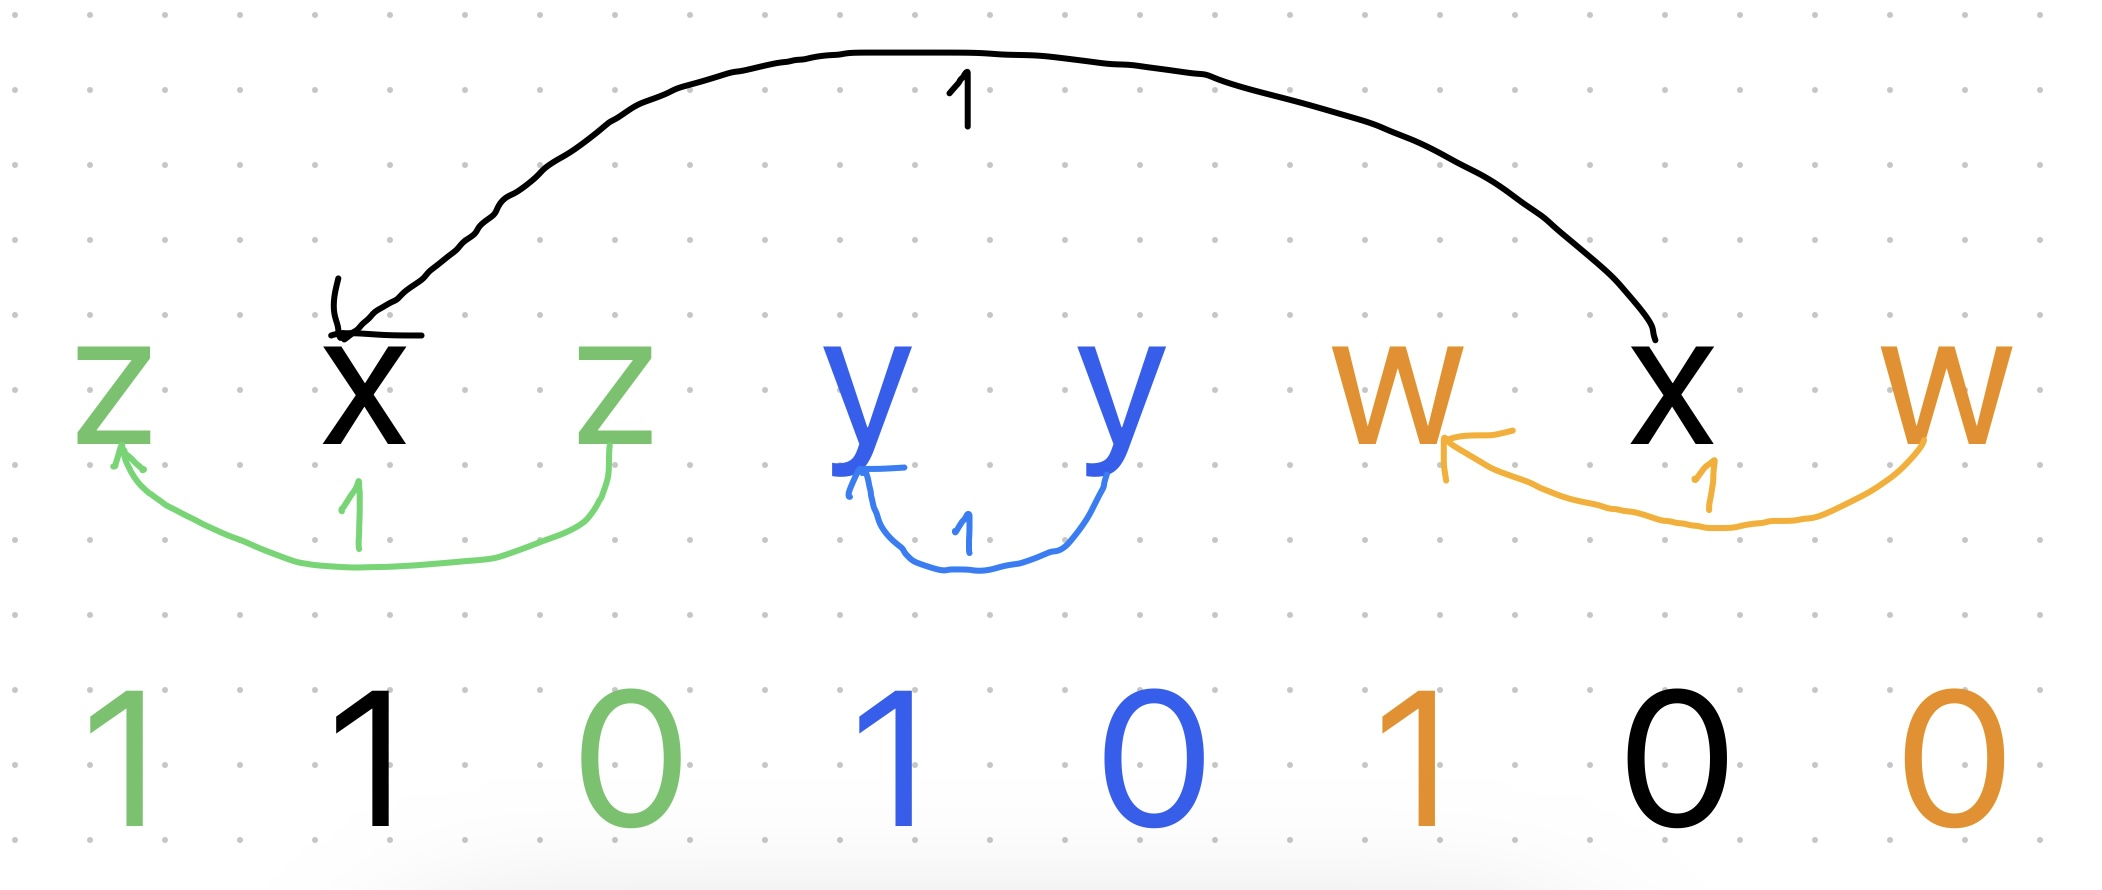
\includegraphics[width=12cm]{nested.jpeg}% Joonise suurus, joonise fail
    \caption{Autori koostatud joonis Freeform abil}% Allkiri
    \allikas{Autori erakogu}% Allikas
    \label{joonis}% Selle järgi viidatakse, pärast käsku \caption
\end{figure}
\end{solution}

\begin{cclol}
#include <bits/stdc++.h>

using namespace std;

#define cint
const int

#pragma GCC optimize("O3,unroll-loops")
#pragma GCC target("avx2,bmi,bmi2,popcnt,lzcnt")

cint MA = 2e5 + 10;

vector < int > t(4 * MA, 0);
int n;

void build() {
  for (int i = n - 1; i > 0; i--) t[i] = t[i << 1] + t[i << 1 | 1];
}

void modify(int x, int val) {
  for (t[x += n] = val; x > 1; x >>= 1) t[x >> 1] = t[x] + t[x ^ 1];
}

int sum(int l, int r) {
  int res = 0;
  for (l += n, r += n; l < r; l >>= 1, r >>= 1) {
    if (l & 1) res += t[l++];
    if (r & 1) res += t[--r];
  }
  return res;
}

int main(int argc, char ** argv) {
  ios_base::sync_with_stdio(false);
  cin.tie(NULL);
  cin >> n;
  n *= 2;
  vector < int > v(n);
  for (int i = 0; i < n; i++) {
    cin >> v[i];
  }
  map < int, pair < int, int >> m;
  vector < int > ans(n / 2);
  for (int i = 0; i < n; i++) {

    m[v[i]].first++;
    if (m[v[i]].first == 1) m[v[i]].second = i;
    if (m[v[i]].first == 2) {
      ans[v[i] - 1] = sum(m[v[i]].second, i + 1);
      modify(m[v[i]].second, 1);
    }
  }
  for (auto u: ans) {
    cout << u << " ";
  }
  return 0;
}
    \end{cclol}
    \begin{kk}[H]
    \caption{Codeforces, Nested segments}% Allkiri
    \allikas{Autori implementatsioon}% Allikas
    \end{kk}
Algoritmi ajakeerukus on $O(N\log N)$.


\subsubsection{Intersecting segments, Codeforces EDU, ***}
\begin{extra}
Ülesannet saab esitada \href{https://codeforces.com/edu/course/2/lesson/4/3/practice/contest/274545/problem/D}{Codeforces platvormi EDU lehel}.
\end{extra}

\begin{prereq}
Loikude puu implementatsioon
\end{prereq}
\begin{Text}
Sisendiks antakse $2n$(kus iga element esineb kaks korda) elementi samamoodi nagu eelmises ülesandes, kuid nüüd on vaja leida elementide arv kujul $xyxy$(iga lõigu kohta), kus $x$ ja $y$ on kindlad elemendid massiivis(ehk leia lõikuvate lõikude arv).

\parencite{inseg}
\end{Text}
\begin{Input}
Esimesel real on $n$$(1\le n\le 10^5)$ täisarvu, teisel real on $2n$ täisarvu. On garanteeritud, et iga arv $1..n$ esineb massiivis kaks korda.
\end{Input}
\begin{Output}
Väljasta $n$ arvu, kus $i$-ndas arv tähistab mitu lõiku lõikuvad lõiguga $i$,
\end{Output}

\textbf{Näidissisend}

\begin{verbatim}
5
5 1 2 2 3 1 3 4 5 4
\end{verbatim}

\textbf{Näidisväljund}

\begin{verbatim}
1 0 1 1 1 
\end{verbatim}


\begin{vihje}
Implementatsioon sarnaneb eelmisele ülesandele.
\end{vihje}

\begin{vihje}
Millistel juhtudel nüüd lisame ja kustutame ühtesi?
\end{vihje}

\begin{vihje}
Mis kasu oleks massiivi mõlemat pidi läbimisest?
\end{vihje}
\begin{solution}
Kasutame taaskord algselt nullidega täidetud massiivi.

Lõikude $x$ ja $y$ kohta saab meil olla kahte eri sorti lõikumisi, $xyxy$ ja $yxyx$.
Esiteks leiame lõikude hulga $x$ kohta, liigume lineaarselt vasakult paremale.
Siis leiame lõikude hulga $y$ kohta, liigume vastupidi, paremalt vasakule.
Mõlemat pidi leitud lõikude summa saab olema meie vastus.
Täpsemalt lõigu $x$ kohta saab meie vastus olema lõikude arv mida me ei ole veel täielikult vaadelnud(näinud ainult vasakut külge), ehk sellised lõigus kus üks pool jääb kahe $x$ vahele.

Algoritm on järgnev:
\begin{itemize}
\item Kui me vaatleme hetkel lõigu vasakult poolt siis märgime selle asukohale ühe.
\item Kui vaatleme paremat poolt, siis leiame summa näiteks lõigu $x$ vahel, ning märgime vasakpoole külje võrdseks nulliga.
\end{itemize}

Autor koostas arusaama toetamiseks ka järgneva joonise, mis kujutab massiivi seisundit parast kõikidele operatsioonidele vastamist:
\begin{figure}[H]% [] sisse märgitakse paigutus H
    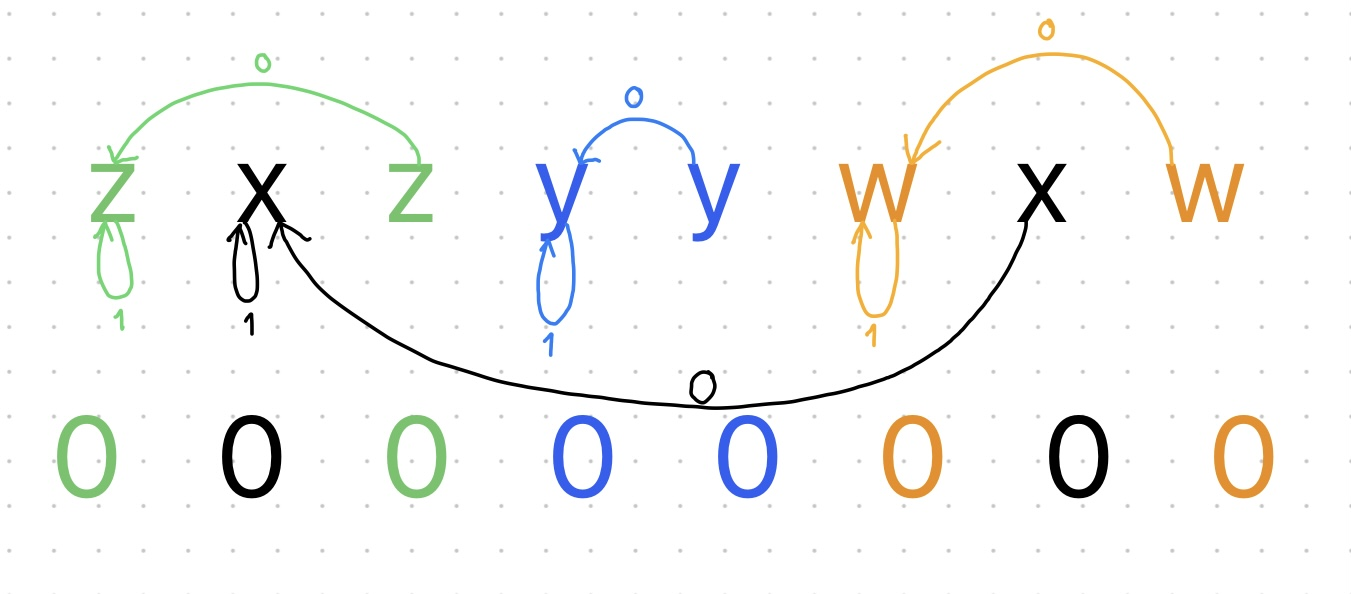
\includegraphics[width=12cm]{intersecting.jpeg}% Joonise suurus, joonise fail
    \caption{Autori koostatud joonis Freeform abil}% Allkiri
    \allikas{Autori erakogu}% Allikas
    \label{joonis}% Selle järgi viidatakse, pärast käsku \caption
\end{figure}

\end{solution}

\begin{cclol}
#include <bits/stdc++.h>

using namespace std;

#define cint
const int

#define pii pair < int, int >
#pragma GCC optimize("O3,unroll-loops")
#pragma GCC target("avx2,bmi,bmi2,popcnt,lzcnt")

cint MA = 2e5 + 10;

vector < int > t(4 * MA, 0);
int n;

void build() {
  for (int i = n - 1; i > 0; i--) {
    t[i] = t[i << 1] + t[i << 1 | 1];
  }
}

void modify(int x, int val) {
  for (t[x += n] = val; x > 1; x >>= 1) t[x >> 1] = t[x] + t[x ^ 1];
}

int sum(int l, int r) {
  int res = 0;
  for (l += n, r += n; l < r; l >>= 1, r >>= 1) {
    if (l & 1) res += t[l++];
    if (r & 1) res += t[--r];
  }
  return res;
}

int main(int argc, char ** argv) {
  ios_base::sync_with_stdio(false);
  cin.tie(NULL);
  cin >> n;
  n *= 2;
  vector < int > v(n);
  for (int i = 0; i < n; i++) cin >> v[i];
  vector < int > ans(n / 2, 0);
  map < int, pii > m;
  for (int i = 0; i < n; i++) {
    m[v[i]].first++;
    if (m[v[i]].first == 1) {
      modify(i, 1);
      m[v[i]].second = i;
    } else if (m[v[i]].first == 2) {
      modify(m[v[i]].second, 0);
      ans[v[i] - 1] += sum(m[v[i]].second, i + 1);
      m[v[i]].first = 0;
    }

  }
  reverse(v.begin(), v.end());
  for (int i = 0; i < n; i++) {
    m[v[i]].first++;
    if (m[v[i]].first == 1) {
      modify(i, 1);
      m[v[i]].second = i;
    } else if (m[v[i]].first == 2) {
      modify(m[v[i]].second, 0);
      ans[v[i] - 1] += sum(m[v[i]].second, i + 1);
    }

  }

  for (auto u: ans) {
    cout << u << " ";
  }
  return 0;
}
    \end{cclol}
    \begin{kk}[H]
    \caption{Codeforces, Intersecting segments}% Allkiri
    \allikas{Autori implementatsioon}% Allikas
    \end{kk}
Ajakeerukus on $O(N\log N)$
\subsubsection{Segment with the maximum sum, Codeforces EDU,  ***}
\begin{extra}
Ülesannet saab esitada \href{https://codeforces.com/edu/course/2/lesson/4/2/practice/contest/273278/problem/A}{Codeforces platvormi EDU lehel}.
\end{extra}
\begin{prereq}
Lõikude puu implementatsioon
\end{prereq}
\begin{Text}
Selles ülesandes on vaja leida lõik mille summa on maksimaalne.

\parencite{9}
\end{Text}
\begin{Input}
Esimesel real on kaks täisarvu arvu $n$ ja $m$$(1\le n, m\le 10^5)$.
Teisel real on $n$ elementi $a_i$$(-10^9\le a_i\le 10^9)$: massiivi $a[]$ algsed väärtused.

Selle järgneb $m$ päringut kujul $i$ $v$, kus peame muutma elemendi indeksiga $i$ väärtuse $v$$(0\le i<n;-10^9\le v\le 10^9)$ väärtuseks.
\end{Input}
\begin{Output}
Väljasta $m+1$ rida: maksimaalse summaga lõik enne operatsioone ja pärast iga operatsiooni. Tähtis on täheldada, et lõik võib ka olla "tühi"(siis oleks summa 0).
\end{Output}

\textbf{Näidissisend 1}

\begin{verbatim}
5 2
5 -4 4 3 -5
4 3
3 -1
\end{verbatim}

\textbf{Näidisväljund 1}

\begin{verbatim}
8
11
7
\end{verbatim}



\textbf{Näidissisend 2}

\begin{verbatim}
4 2
-2 -1 -5 -4
1 3
3 2
\end{verbatim}

\textbf{Näidisväljund 2}

\begin{verbatim}
0
3
3
\end{verbatim}


\begin{vihje}
Igas tipus peab salvestama mitut erinevat tüüpi informatsiooni.
\end{vihje}

\begin{vihje}
Joonista paberil näiteid, võibolla on märgata mis seaduspärad kehtivad tippude uuendamisel.
\end{vihje}

\begin{solution}
Ütleme, et meil on lõik $x$, mis on jagatud kaheks võrdseks pooleks.
Me tahame lõigu $x$ kohta leida väärtuse $seg$: maksimaalne alamlõigu summa lõigul. Teades ainult $seg_1$ ja $seg_2$ (vastused mõlema lõigu kohta) me ei saa kohe leida $seg$ väärtust, põhjusel, et suurima summaga lõik võib läbida mõlemat lapstipu lõiku.
Teame, et sellise lõikumise korral koosneb optimaalne alamlõik vasakpoolse lõigu suffiksist ja parempoolse lõigu prefiksist.
Hoiame mõlema lõigu kohta veel kahte väärtust: $pref$ ja $suf$: prefiks ja suffiks maksimaalse väärtusega. Siis saad leida $seg$ järgnevalt: $seg=max(seg_1,seg_2,suf_1+pref_2)$.


\begin{figure}[H]% [] sisse märgitakse paigutus H
    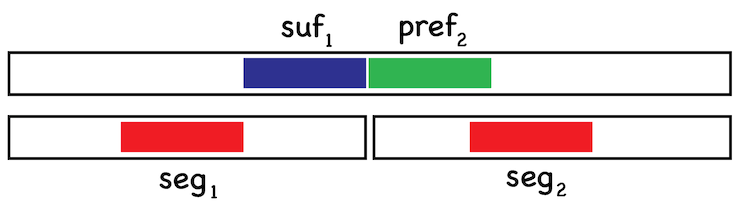
\includegraphics[width=12cm]{sumseg.png}% Joonise suurus, joonise fail
    \caption{Joonis mis kujutab lõikude prefikseid ja suffikseid}% Allkiri
    \allikas{Codeforces EDU}% Allikas
    \label{joonis}% Selle järgi viidatakse, pärast käsku \caption
\end{figure}

Nüüd peame arvutama $pref$ ja $suf$.
$pref$ ja $suf$ leitakse sarnaselt.
Maksimaalne prefiks on võrdne, kas vasakpoolse lõigu maksimaalse prefiksiga, või koosneb tervest vasakust lõigust ja maksimaalsest prefiksist paremal pool.
Lisame veel iga tipu kohta väärtuse $sum$, mis on võrdne summaga lõigul. Siis $pref=max(pref_1,sum_1+pref_2)$, sarnaselt $suf=max(suf_2,sum_2+suf_1)$.
Lõpuks saame leida $sum$ valemiga: $sum=sum_1+sum_2$.
Sarnaselt, saame lisada andmestruktuurile lisaoperatsiooni $max\_subsegment(l,r)$: leia maksimaalse summaga lõik vahemikus $l..r$.
\end{solution}

\begin{cclol}
#include <bits/stdc++.h>

using namespace std;
#define ll long long
#define max3(a, b, c) max(max(a, b), c)
struct tre {
  ll suf, pref, seg, sum;
};
vector < tre > tree(400001);
tre merge(tre a, tre b) {
  tre t = {
    max(b.suf, b.sum + a.suf),
    max(a.pref, a.sum + b.pref),
    max3(a.seg, b.seg, a.suf + b.pref),
    a.sum + b.sum
  };
  return t;
}
void build_tree(ll int * a, ll int s, ll int e, ll int index) {
  if (s == e) {
    if (a[s] > 0)
      tree[index] = {
        a[s],
        a[s],
        a[s],
        a[s]
      };
    else
      tree[index] = {
        0,
        0,
        0,
        a[s]
      };
    return;
  }
  ll int mid = (s + e) / 2;
  build_tree(a, s, mid, 2 * index);
  build_tree(a, mid + 1, e, 2 * index + 1);
  tree[index] = merge(tree[2 * index], tree[2 * index + 1]);
  return;
}

void point_update(ll ss, ll  se, ll i, ll inc, ll index) {
  if (i > se || i < ss)
    return;
  if (ss == se) {
    if (inc > 0)
      tree[index] = {
        inc,
        inc,
        inc,
        inc
      };
    else
      tree[index] = {
        0,
        0,
        0,
        inc
      };
    return;
  }
  ll int mid = (ss + se) / 2;
  point_update(ss, mid, i, inc, 2 * index);
  point_update(mid + 1, se, i, inc, 2 * index + 1);
  tree[index] = merge(tree[2 * index], tree[2 * index + 1]);
  return;
}

void solve() {
  int n, q;
  cin >> n >> q;

  ll a[n];
  for (int i = 0; i < n; i++)
    cin >> a[i];

  build_tree(a, 0, n - 1, 1);
  cout << tree[1].seg << endl;

  while (q--) {
    ll num, l;
    cin >> num >> l;
    point_update(0, n - 1, num, l, 1);
    cout << tree[1].seg << endl;
    a[num] = l;
  }

}
int main() {
  ios_base::sync_with_stdio(false);
  cin.tie(NULL);

  ll int t = 1;
  while (t--) {
    solve();
  }

  return 0;
}
\end{cclol}
 \begin{kk}[H]% [] sisse märgitakse paigutus H
    \caption{Rekursiivne implementatsioon ülesandele Segment with the maximum sum}% Allkiri
    \allikas{Manan Ghetia GitHub}% Allikas
    \label{EMaxx}% Selle järgi viidatakse, pärast käsku \caption
    \end{kk}
Ajakeerukus on $O(N\log N)$.

\subsubsection{Kaardid, EIO 2022/23 II valikvõistlus, ****}
\begin{extra}
Ülesannet kahjuks ei saa enam esitada, kuid \href{eio.ee}{EIO} lehel on olemas testid ülesandele.
\end{extra}
\begin{prereq}
Laisk laienemine
\end{prereq}
\begin{Text}
.pdf fail ülesandest on täismahus kättesaadav(vt Lisa 15). \parencite{10}
\end{Text}

Võistlusel piisas kahe esimese alamülesande lahendamiseks naiivsest jõumeetodist.
Autori implementatsioon jäi viimases alamülesandes ajahätta maksimaalselt $0,1$ sekundiga.
 \begin{cclol}
#include <bits/stdc++.h>

using namespace std;

#pragma GCC optimize("O3,unroll-loops")
#pragma GCC target("avx2,bmi,bmi2,popcnt,lzcnt")

int m[25001];

int main() {
  ios_base::sync_with_stdio(false);
  cin.tie(NULL);
  int n;
  cin >> n;
  vector < int > v(6 * n);
  for (int i = 0; i < 3 * n; i++) {
    cin >> v[i];
  }
  for (int i = 0; i < 3 * n; i++) {
    v[i + 3 * n] = v[i];
  }
  vector < pair < int, int >> a;

  for (int j = 0; j < 3 * n; j++) {
    int tAns = 0;
    int cards = 0;
    for (int i = j; i < j + 3 * n; i++) {
      m[v[i]]++;
      if (m[v[i]] == 3) {
        m[v[i]] = 0;
        cards -= 2;
      } else {
        cards++;
      }
      tAns = max(tAns, cards);
    }
    a.pb({
      tAns,
      j + 1
    });
    memset(m, 0, sizeof(m));
  }
  sort(a.begin(), a.end());
  cout << a[0].first << " ";
  int cc = 0;
  for (auto u: a) {
    if (u.first == a[0].first) cc++;
    else break;
  }
  cout << cc << endl;
  for (auto u: a) {
    if (u.first == a[0].first) cout << u.second << " ";
    else break;
  }
  return 0;
}
    \end{cclol}
    \begin{kk}[H]
    \caption{44 punkti kood}% Allkiri
    \allikas{Autori implementatsioon}% Allikas
    \end{kk}

Kood teeb halvimal juhul $(N^2)/2$ operatsiooni ehk ajakeerukuseks on $O(N^2)$.

\begin{solution}
$100$ punkti lahendus kasutab laiska laienemeist lõikude puul. 
Laisa laienemise vajadus tuleneb sellest, et ülesandes on vaja teha nii lõigu uuendamisoperatsioone kui ka lõigu väärtuse saamise operatsioone(inglise keeles Range Update Range Query).

Ülesande lahendamiseks on vaja uuendada vahemikku, et märkida ära mitu kaardi sul on käes mingis kindlas vahemikus(liites või lahutades 1).
Seejärel saab vaadata uuesti massiivilt, mis on uus maksimum(soovime leida maksimaalse arvu kaarte, mis meil on käes kui alustada mingist indeksist kaartide korjamist).

Selline lahendus võtab halvimal juhul aega $0,2$ sekundit, ning omab ajakeerukust $O(N\log N)$.
\end{solution}
\begin{cclol}
#include<iostream>

#include<vector>

#include<cmath>

#include<unordered_map>

#include<algorithm>

#define INT_MAX 1e9 + 5

#define left(i)(i << 1) + 1
#define right(i)(i << 1) + 2

using namespace std;

typedef vector < int > vi;
typedef vector < vi > vvi;
typedef unordered_map < int, vi > mp_ivi;

class SegmentTree {
  private: vi tree,
  lazy;
  int n;
  public: SegmentTree(int sz) {
    n = sz;
    tree.assign(4 * n, 0);
    lazy.assign(4 * n, 0);
  }

  void propagate(int idx, int l, int r) {
    tree[idx] += lazy[idx];
    if (l != r) {
      lazy[right(idx)] += lazy[idx];
      lazy[left(idx)] += lazy[idx];
    }
    lazy[idx] = 0;
  }

  void update_range(int idx, int l, int r, int L, int R, int val) {
    propagate(idx, l, r);
    if (l > r || r < L || R < l || R < L) return;
    if (L <= l && r <= R) {
      lazy[idx] += val;
      propagate(idx, l, r);
    } else {
      int mid = (l + r) / 2;
      update_range(left(idx), l, mid, L, min(mid, R), val);
      update_range(right(idx), mid + 1, r, max(mid + 1, L), R, val);
      tree[idx] = max(tree[left(idx)], tree[right(idx)]);
    }
  }

  void update_range(int l, int r, int val) {
    update_range(0, 0, n - 1, l, r, val);
  }

  int max_query(int idx, int l, int r, int L, int R) {
    propagate(idx, l, r);
    if (l > r || r < L || R < l || R < L) return -1;
    if (L <= l && r <= R) {
      return tree[idx];
    } else {
      int mid = (l + r) / 2;
      return max(
        max_query(left(idx), l, mid, L, min(mid, R)),
        max_query(right(idx), mid + 1, r, max(mid + 1, L), R)
      );
    }
  }

  int max_query(int l, int r) {
    return max_query(0, 0, n - 1, l, r);
  }
};

int main() {
  ios_base::sync_with_stdio(false);
  cin.tie(0);

  int n;
  cin >> n;
  SegmentTree st(3 * n);

  vi cards(3 * n);
  vvi positions(n + 1);

  for (int i = 0; i < 3 * n; i++) {
    int a;
    cin >> a;
    cards[i] = a;
    positions[a].push_back(i);
  }

  for (int i = 1; i <= n; i++) {
    vi & tmp = positions[i];
    st.update_range(tmp[0], tmp[2] - 1, 1);
    st.update_range(tmp[1], tmp[2] - 1, 1);
  }

  vvi minimal_positions(3 * n + 1);
  vi cur_starts(n + 1, 0);
  int min_val = INT_MAX;

  for (int i = 0; i < 3 * n; i++) {
    vi & tmp = positions[cards[i]];
    int cur_start = cur_starts[cards[i]];
    cur_starts[cards[i]]++;

    int swappable = (cur_start + 2) % 3;
    if (cur_start < swappable) {
      st.update_range(tmp[cur_start], tmp[swappable] - 1, -1);
      st.update_range(tmp[swappable], 3 * n - 1, 2);
      st.update_range(0, tmp[cur_start] - 1, 2);
    } else {
      st.update_range(tmp[cur_start], 3 * n - 1, -1);
      st.update_range(0, tmp[swappable] - 1, -1);
      st.update_range(tmp[swappable], tmp[cur_start] - 1, 2);
    }
    int tmpi = st.max_query(0, 3 * n - 1);
    if (i + 2 > 3 * n)
      minimal_positions[tmpi].push_back(1);
    else
      minimal_positions[tmpi].push_back(i + 2);
    min_val = min(min_val, tmpi);
  }
  vi & minimal_pos = minimal_positions[min_val];
  int s = min_val, k = minimal_pos.size();
  cout << s << ' ' << k << '\n';
  sort(minimal_pos.begin(), minimal_pos.end());
  for (int i = 0; i < k - 1; i++) {
    cout << minimal_pos[i] << ' ';
  }
  cout << minimal_pos[k - 1] << '\n';

  return 0;
}
\end{cclol}
 \begin{kk}[H]
    \caption{100 punkti kood}% Allkiri
    \allikas{Kaasvõistleja Marten Mehide lahendus}% Allikas
    \end{kk}


\subsubsection{Subtree Queries, CSES, ****}
\begin{extra}
Ülesannet saab esitada \href{https://cses.fi/problemset/task/1137}{CSES platvormil}.
\end{extra}
\begin{prereq} 
Euler'i ringreisi leidmine graafis, puud, lõikude puu implementatsioon, sügavuti läbimine
\end{prereq}
\begin{Text}
Meil on $n$ tipuga juuritud. Tipud on nummerdatud $1,2,...,n$, ja tipp $1$ on juurtipp. Igal tipul on väärtus. 

Peame täitma päringuid kujul:
\begin{itemize}
\item $1$ $s$ $x$: muuda tipu $s$ väärtus $x$-i väärtuseks. 
\item $2$ $s$: leia tipu $s$ alampuu tippude väärtuste summa.
\end{itemize}

\parencite{13}
\end{Text}
\begin{Input}
Esimesel real on kaks täisarvu arvu $n$ ja $q$$(1\le n,q\le 2\cdot10^5)$: tippude arv ja päringute arv.

Teisel real on $n$ täisarvu $v_1,v_2,...,v_n$: iga tipu $1..n$ väärtused$(1\le v_i,x\le 10^9)$.

Sellele järgneb $n-1$ rida kujul $a$ $b$$(1\le a,b,s\le n)$, mis tähistab külge tippude $a$ ja $b$ vahel.

Seejärel on $q$ rida päringuid kujul $1\ s\ x$ või $2\ s$.
\end{Input}
\begin{Output}
Väljasta iga teist tüüpi päringu vastus.
\end{Output}

\textbf{Näidissisend}

\begin{verbatim}
5 3
4 2 5 2 1
1 2
1 3
3 4
3 5
2 3
1 5 3
2 3
\end{verbatim}

\textbf{Näidisväljund}

\begin{verbatim}
8
10
\end{verbatim}



Näidissisend vastab kujutatud graafile:
\begin{figure}[H]% [] sisse märgitakse paigutus H
    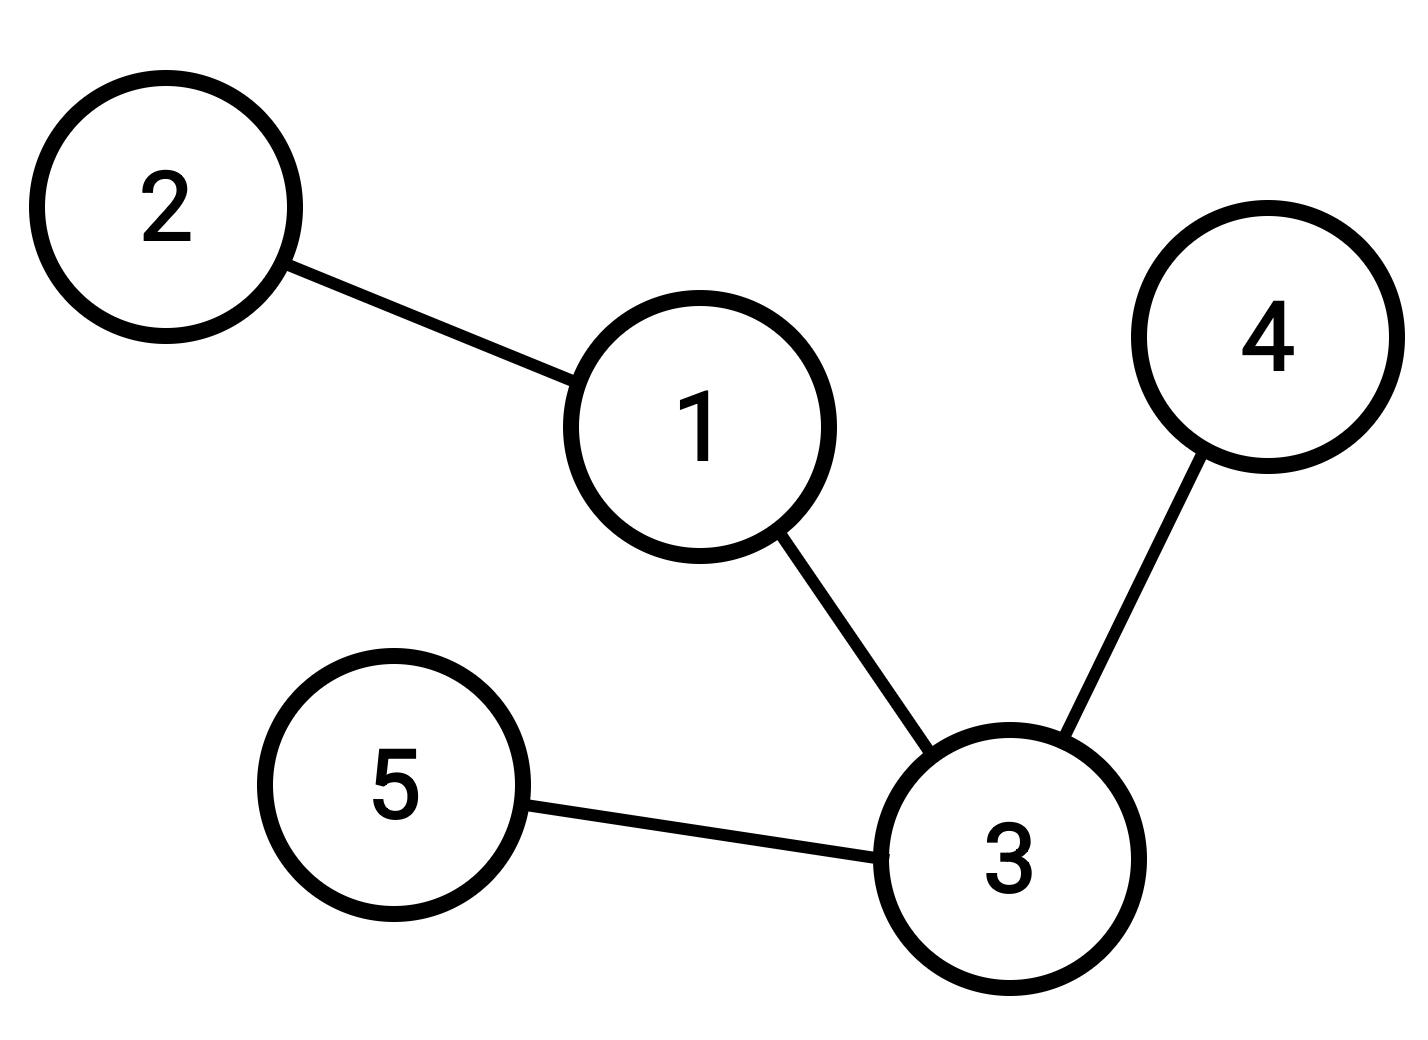
\includegraphics[width=10cm]{ntpuu.jpeg}% Joonise suurus, joonise fail
    \caption{Näidispäringule vastav puu}% Allkiri
    \allikas{USACO Guide}% Allikas
    \label{joonis}% Selle järgi viidatakse, pärast käsku \caption
\end{figure}

\begin{vihje}
Leia Euler'i ringreis.    
\end{vihje}

\begin{vihje}
Kasuta abimassiive.
\end{vihje}

\begin{vihje}
Kasuta lõikude puu standardseid operatsioone, et leida summasid ja muuta väärtusi sellel puul.
\end{vihje}

\begin{solution}
Alustuseks jooksutame puul sügavuti otsingut, et leida Euler'i ringreis.
Selle tulemusena saame $[\texttt{st}[i], \texttt{en}[i]]$, mis sisaldab kõiki vahemike $[\texttt{st}[j] ja \texttt{en}[j]]$ iga $j$ kohta $i$ alampuus. Samuti, $\texttt{en}[i]-\texttt{st}[i]+1$ on võrdne alampuu $i$ suurusega.
\begin{cclol}
const int MX = 2e5 + 5;
vector < int > adj[MX];
int timer = 0, st[MX], en[MX];

void dfs(int node, int parent) {
  st[node] = timer++;
  for (int i: adj[node]) {
    if (i != parent) {
      dfs(i, node);
    }
  }
  en[node] = timer - 1;
}
\end{cclol}
\begin{kk}[H]% [] sisse märgitakse paigutus H
    \caption{Implementatsioon}% Allkiri
    \allikas{USACO Guide}% Allikas
    \label{EMaxx}% Selle järgi viidatakse, pärast käsku \caption
    \end{kk}
    
Kasutame selgitamisel ka varasemat näidispäringut.

Enne sügavuti otsingut, on massiivid $\texttt{st}$ ja $\texttt{en}$ täidetud nullidega. 
Järgnevas visualisatsioonis, tähistab esimene rida tippude indekseid, teine rida tähistab $\texttt{st}$, ning kolmas tähistab $\texttt{en}$.

Käime nüüd operatsioonid ükshaaval läbi:

\begin{figure}[H]% [] sisse märgitakse paigutus H
    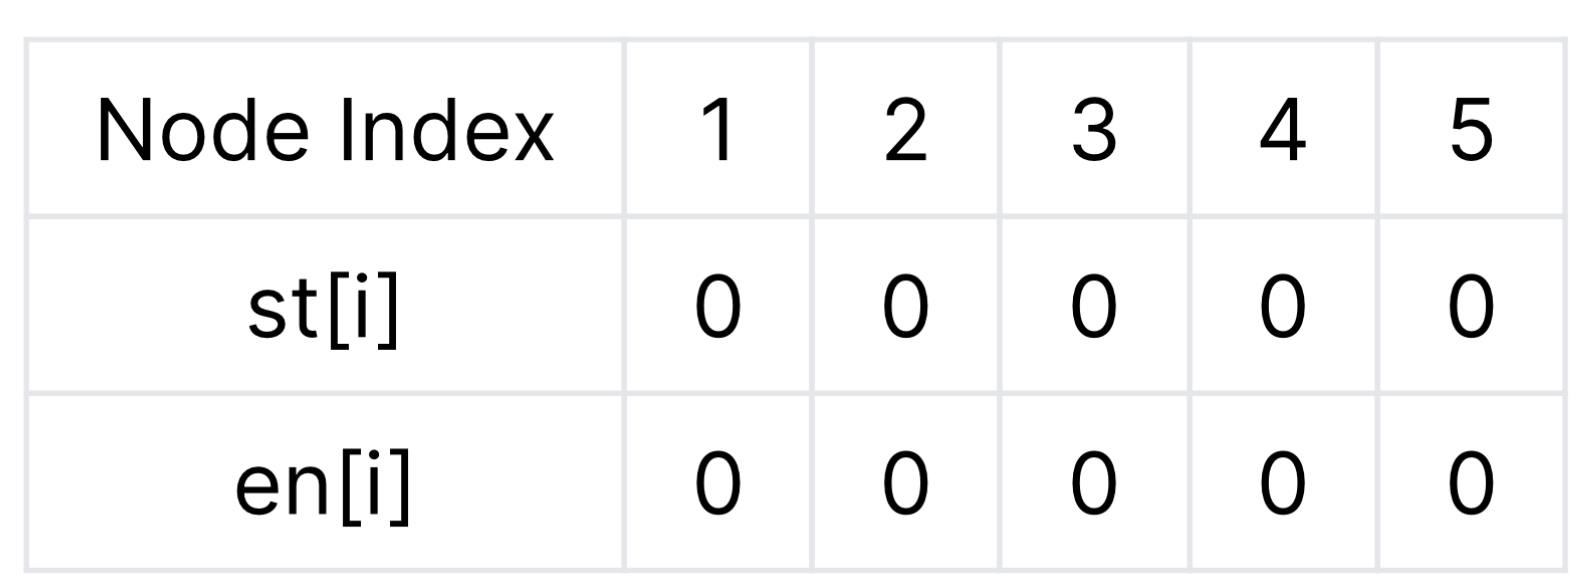
\includegraphics[width=12cm]{first.jpeg}% Joonise suurus, joonise fail
    \caption{Massiiv kui timer on 0}% Allkiri
    \allikas{USACO Guide}% Allikas
    \label{joonis}% Selle järgi viidatakse, pärast käsku \caption
\end{figure}

Seepärast et kutsume $\text{dfs}(1, 0)$, me muudame $\texttt{st}[1]$ võrdseks praeguse timer'i väärtusega $0$. Seejärel kutsume funktsioonid $\text{dfs}(2, 1)$ ja
$\text{dfs}(3, 1)$.

\begin{figure}[H]% [] sisse märgitakse paigutus H
    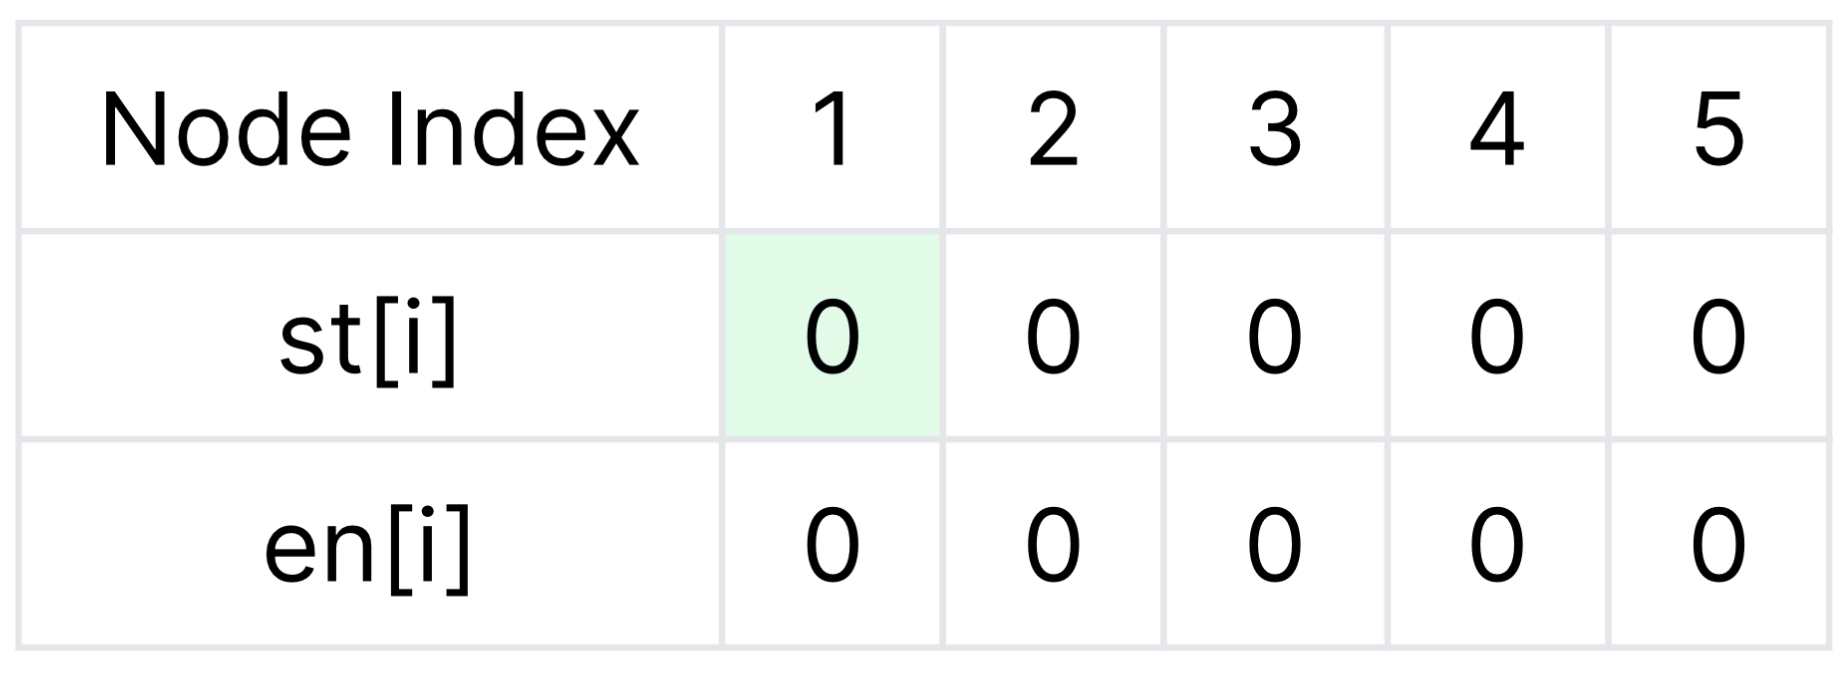
\includegraphics[width=12cm]{second.jpeg}% Joonise suurus, joonise fail
    \caption{Massiiv kui timer on 1}% Allkiri
    \allikas{USACO Guide}% Allikas
    \label{joonis}% Selle järgi viidatakse, pärast käsku \caption
\end{figure}

Nüüd $\text{dfs}(2, 1)$ ja $\text{dfs}(3, 1)$. 
See ei ole tähtis mis järjekorras me neid operatsioone teeme, ehk alustame,
$\text{dfs}(2, 1)$. Põhjusel, et taimeri väärtus on 1, me teeme $\texttt{st}[2]=1$ ja suurendame taimeri väärtust ühe võrra. Kuid, sellepärast, et tipul $2$ ei ole lapsi, me ei kutsu
$\text{dfs}$. Selle asemel, me teeme $\texttt{en}[2]=1$, sest taimeri praegune väärtus on 2.

\begin{figure}[H]% [] sisse märgitakse paigutus H
    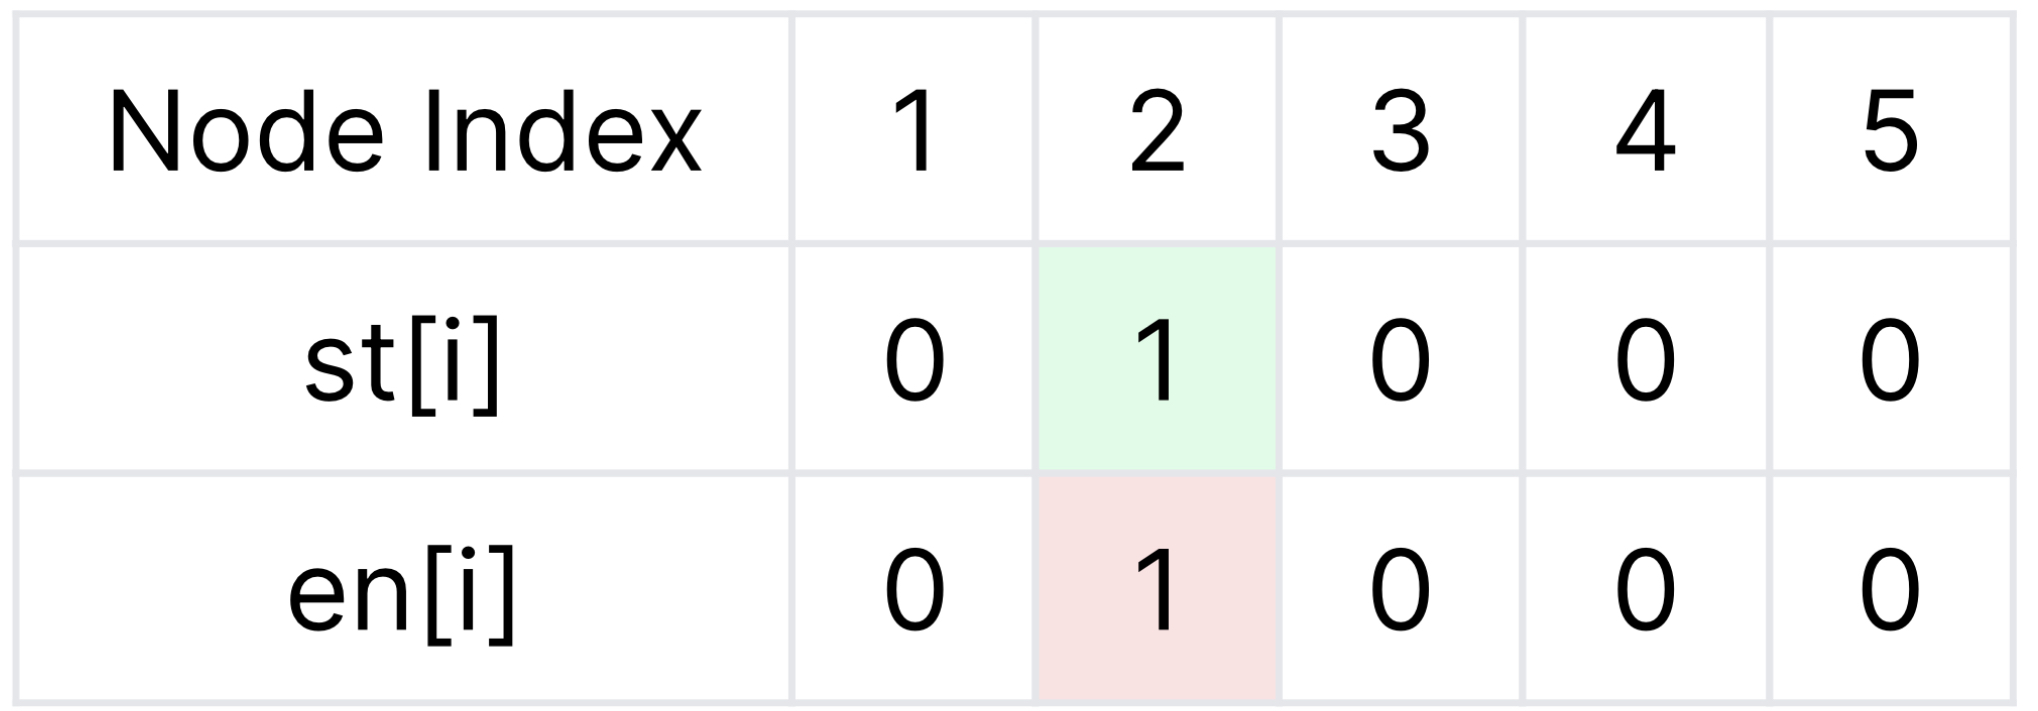
\includegraphics[width=12cm]{third.jpeg}% Joonise suurus, joonise fail
    \caption{Massiiv kui timer on 2}% Allkiri
    \allikas{USACO Guide}% Allikas
    \label{joonis}% Selle järgi viidatakse, pärast käsku \caption
\end{figure}

Nüüd teeme $\text{dfs}(3, 1)$. 
Nagu ennegi, me muudame
$\texttt{st}[3]$ väärtuse võrdseks taimeri väärtusega(praegusel juhul 2) ja suurendamine taimeri väärtust ühe võrra. 
Seejärel, kutsume funktsioonid $\text{dfs}(4, 3)$ ja
$\text{dfs}(5, 3)$.

\begin{figure}[H]% [] sisse märgitakse paigutus H
    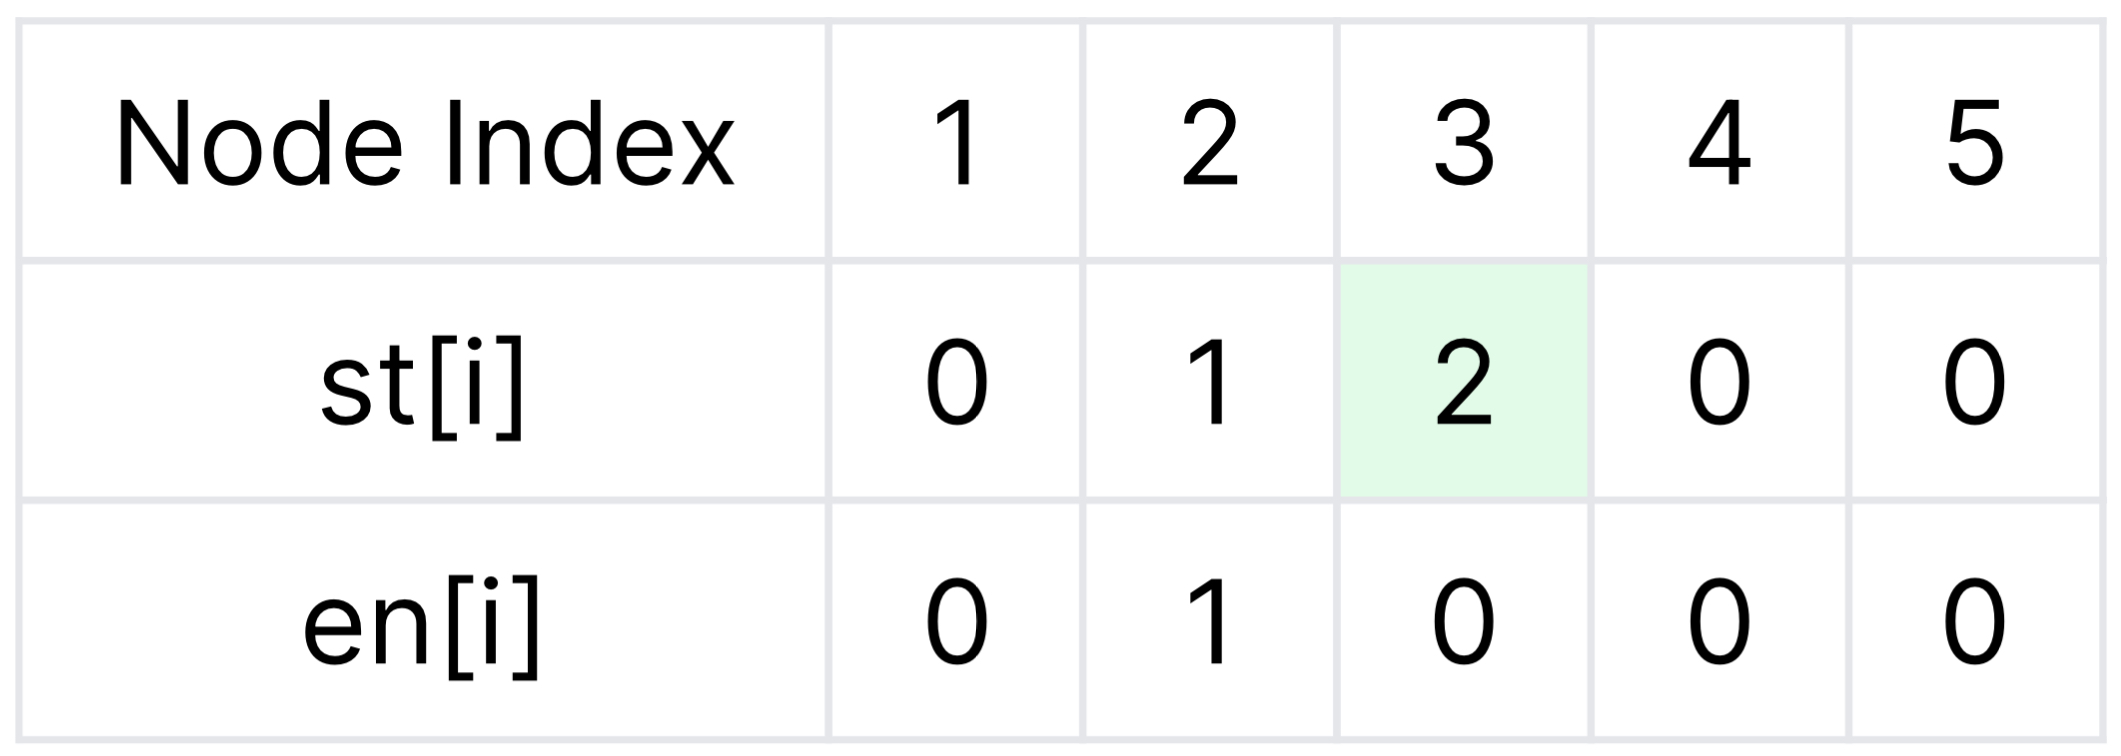
\includegraphics[width=12cm]{fourth.jpeg}% Joonise suurus, joonise fail
    \caption{Massiiv kui timer on 3}% Allkiri
    \allikas{USACO Guide}% Allikas
    \label{joonis}% Selle järgi viidatakse, pärast käsku \caption
\end{figure}

Nüüd käsitleme kutsumisi $\text{dfs}(4, 3)$ ja $\text{dfs}(5, 3)$. 
Esiteks, me teeme $\text{dfs}(4, 3)$ muutes $\texttt{st}[4]$ võrdseks taimeri väärtusega(praegusel juhul 3) ja suurendades taimeri väärtust ühe võrra. 
Siis, sest tipul $4$ pole lapsi, teeme $\texttt{en}[4]=3$.

Nüüd on taimeri väärtus 4, and we $\text{dfs}(5, 3)$. Sarnaselt eelnevaga, teeme $\texttt{st}[5]=4$. 
Tipp $5$ puuduvad lapsed,
teeme $\texttt{en}[5]=4$.


\begin{figure}[H]% [] sisse märgitakse paigutus H
    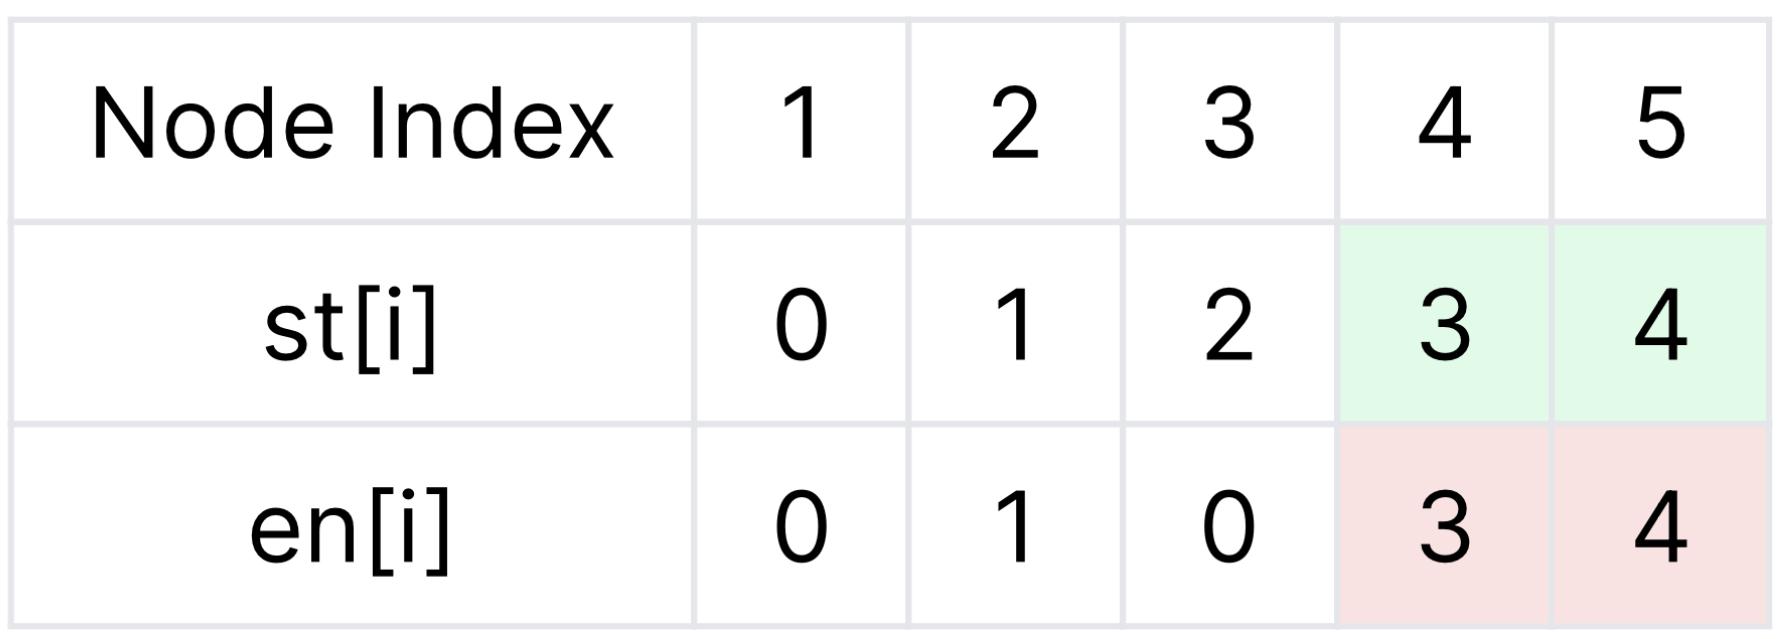
\includegraphics[width=12cm]{fifth.jpeg}% Joonise suurus, joonise fail
    \caption{Massiiv kui timer on 5}% Allkiri
    \allikas{USACO Guide}% Allikas
    \label{joonis}% Selle järgi viidatakse, pärast käsku \caption
\end{figure}
Nüüd lõpetuseks teeme $\texttt{en}[\text{node}] = \text{timer} - 1$
kutsumisi. Esiteks lahendame tipp $3$, tehes $\texttt{en}[3]=4$.Teeme sama tipp $1$ juhul, $\texttt{en}[1]=4$. 
Nüüd on sügavuti otsing lõppenud.
\begin{figure}[H]% [] sisse märgitakse paigutus H
    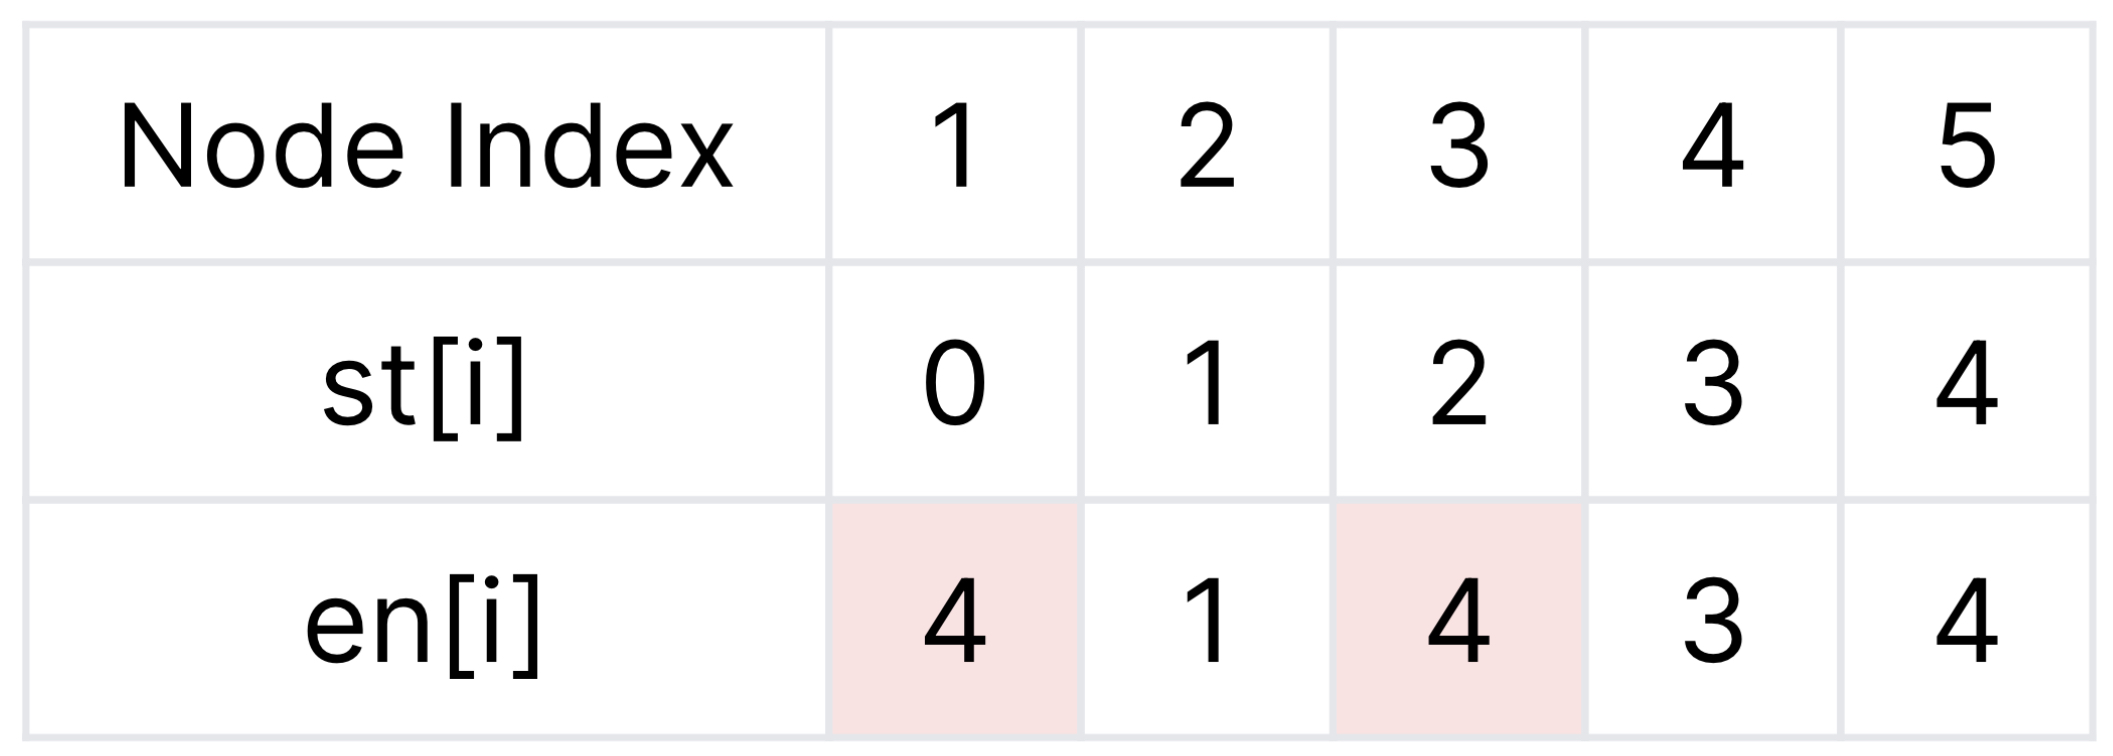
\includegraphics[width=12cm]{sixth.jpeg}% Joonise suurus, joonise fail
    \caption{Massiiv kui timer on 5}% Allkiri
    \allikas{USACO Guide}% Allikas
    \label{joonis}% Selle järgi viidatakse, pärast käsku \caption
\end{figure}
\end{solution}
Kasutame lõikude puud, et leida summasid ja muuta elementide väärtuseid:
\begin{cclol}
template < class T > struct Seg { // comb(ID,b) = b
  const T ID = 0;
  T comb(T a, T b) {
    return a + b;
  }
  int n;
  vector < T > seg;
  void init(int _n) {
    n = _n;
    seg.assign(2 * n, ID);
  }
  void pull(int p) {
    seg[p] = comb(seg[2 * p], seg[2 * p + 1]);
  }
  void upd(int p, T val) { // set val at position p
    seg[p += n] = val;
    for (p /= 2; p; p /= 2) pull(p);
  }
  T query(int l, int r) { // sum on interval [l, r]
    T ra = ID, rb = ID;
    for (l += n, r += n + 1; l < r; l /= 2, r /= 2) {
      if (l & 1) ra = comb(ra, seg[l++]);
      if (r & 1) rb = comb(seg[--r], rb);
    }
    return comb(ra, rb);
  }
};

Seg < ll > S;
int v[MX];

int main() {
  int n, q;
  cin >> n >> q;
  FOR(i, 1, n + 1) cin >> v[i];
  F0R(i, n - 1) {
    int a, b;
    cin >> a >> b;
    adj[a].pb(b), adj[b].pb(a);
  }
  dfs(1, 0);
  S.init(n);
  FOR(i, 1, n + 1) S.upd(st[i], v[i]);
  F0R(i, q) {
    int t;
    cin >> t;
    if (t == 1) {
      int s, x;
      cin >> s >> x;
      S.upd(st[s], x);
    } else {
      int s;
      cin >> s;
      cout << S.query(st[s], en[s]) << "\n";
    }
  }
}
\end{cclol}
\begin{kk}[H]% [] sisse märgitakse paigutus H
    \caption{Rekursiivne lahendus ülesandele Subtree Queries}% Allkiri
    \allikas{USACO Guide}% Allikas
    \label{EMaxx}% Selle järgi viidatakse, pärast käsku \caption
    \end{kk}


\begin{extra}
Rohkem sarnaseid ülesandeid leidub USACO Guide Gold alapeatükis Trees.
\end{extra}


\subsubsection{Counting Haybales, USACO Platinum 2015 detsember, *****}
\begin{extra}
Ülesannet saab esitada \href{http://www.usaco.org/index.php?page=viewproblem2&cpid=578}{USACO ametlikul veebilehel}.
\end{extra}
\begin{prereq}
Laisk laienemine
\end{prereq}
\begin{Text}
Põllumees Joonas proovib palgata töölisi kes korraldaksid asju ümber tema talus, aga siiamaani on kõik alla andnud nähes keerulisi juhiseid mida Põllumees Joonas nõudis, et nad järgiks. Jäetud üksipäi, ta saab aru, et ta on võibolla teinud projekti keerulisemaks kui vajalik. Palun aita tal järgida oma enda juhiseid, et lõpetada projekt.

Põllumees Joonase talu koosneb $N$ põllumaast mis on ridamisi, nummerdatud $1...N$. Igal põllumaal saab olla ükskõik mis arv heinakuhje.
Põllumees Joonase juhised jaotuvad järgnevalt:
\begin{itemize}
    \item Antud lõik põllumaid, lisa igale põllumaale üks heinakuhi.
    \item Antud lõik põllumaid,  leia minimaalne arv heinakuhje põllumaadel antud vahemikus.
    \item Antud lõik põllumaid,  leia mitu heinakuhja on antud vahemikus kokku.
\end{itemize}

\parencite{11}
\end{Text}
\begin{Input}
Esimesel real on antud kaks positiivset täisarvu, $N$($1\le N\le 2\cdot 10^5$) ja $Q$($1\le Q\le 10^5$).

Järgneb $N$ rida millel on mitte-negatiivsed täisarvud suurusjärgus kuni $10^5$,  millest igaüks tähistab mitu heinakuhja on algselt igal põllumaal.

Järgmisel $Q$ real on üks kirjatäht(M, P või S), ning kaks positiivset täisarvu $A$ ja $B$($1\le A\le B\le N$), või kolm positiivset täisarvu $A, B$ ja $C$($1\le A\le B\le N$; $1\le C\le 10^5$). Kolm positiivset täisarvu antakse ainult juhul kui eelnevalt antud kirjatäht oli P.

\end{Input}
\begin{Output}
\begin{itemize}
    \item Kui antud kirjatäht on M, väljasta minimaalne arv heinakuhje vahemikus $A...B$.
    \item Kui antud kirjatäht on P,  lisa $C$ heinakuhja igale põllumaale vahemikus $A...B$.
    \item Kui antud kirjatäht on S, väljasta mitu heinakuhja on vahemikus $A...B$  kokku.
\end{itemize}
\end{Output}



\textbf{Näidissisend}

\begin{verbatim}
4 5
3 1 2 4
M 3 4
S 1 3
P 2 3 1
M 3 4
S 1 3
\end{verbatim}

\textbf{Näidisväljund}

\begin{verbatim}
2
6
3
8
\end{verbatim}


\begin{solution}
Selles ülesandes antakse meile $N$ täisarvust koosnev loend ja peame toetama kolme järgnevat päringutüüpi:

\begin{enumerate}
    \item Arvutage loendis oleva intervalli minimaalne arv.
    \item Arvutage loendis oleva intervalli kõigi arvude summa.
    \item Suurenda loendi intervalli iga arvu mõne arvu $K$ võrra.
\end{enumerate}

Alustuseks kirjeldame andmestruktuuri, mis toetab kahte esimest päringutüüpi $O(\log N)$ ajakeerukusega.

Arvestades esialgset loendit, säilitame teatud intervallide hulga jaoks minimaalse arvu selles intervallis ja kõigi selle intervalli arvude summa. 

Kasutatavate intervallide loend on järgmine:
\begin{itemize}
    \item $[1,N]$ on hulgas.
    \item Kui $[a,b]$ on hulgas $a<b$-ga, siis $c=⌊{(a+b)}/2⌋$, $[a,c]$ ja $[c+1,b]$ on hulgas.
\end{itemize}


On hea täheldada ,et selles hulgas on $O(N)$ intervalle. 
Lihtsuse huvides saab ette kujutada, et me ehitame kahendpuu, kus puu juur vastab intervallile $[1,N]$ ja selle miinimumile/summale, puude lehed on kõik intervallid kujul $[i,i]$ nende miinimumide/summadega, ning intervalli $[a,b]$ vasak ja parem lapstipp on vastavalt $[a,c]$ ja $[c+1,b]$.

Arvestades intervallide $[a,c]$ ja $[c+1,b]$ miinimumi, on intervalli $[a,b]$ miinimum nende kahe minimaalne väärtus. Sarnase loogika järgi on intervalli $[a,b]$ summa intervallide $[a,c]$ ja $[c+1,b]$ summa.

Kirjeldame nüüd üksikasjalikult, kuidas esimest operatsiooni toetada – teist operatsiooni toetatakse väga sarnase loogikaga.

Arvestades intervalli $[l,r]$, mille jaoks tahame arvutada selle intervalli minimaalse arvu, kaaluge üldiselt, kuidas puu konkreetne intervall võib aidata meil vastata esimesele päringule. Kui selle sõlme intervall on rangelt meie intervalli sees, siis selle intervalli miinimum on selle intervalli minimaalse arvu "kandidaat" ja me ei pea selle lapsi kontrollima. Kui intervall selles sõlmes on rangelt väljaspool seda intervalli, siis ignoreerime seda intervalli. Vastasel juhul peame rekursiivselt vaatama intervalli kahte last. Kui oleme puu läbi otsimise lõpetanud, tagastame lihtsalt minimaalse kandidaadi.

Kui alustame seda protsessi juurest, võib puu iga tase anda maksimaalselt kaks kandidaati ja me saame naasta ainult kahest teisest sõlmest puu madalamale tasemele. Kui puu antud tasemelt oleks leitud kolm kandidaati, siis kahel neist kandidaatidest peaks olema ühine vanem ja oleksime võinud analüüsi lühendada, kontrollides just seda intervalli. Samamoodi peavad tipud, kus me pöörduksime tagasi madalamale tasemele, olema kehtivast kandidaadist otse vasakul või paremal. Seetõttu kontrollime ainult $O(\log N)$ tippu.

Teine operatsioon toimib sisuliselt samamoodi, ainult et me liidame "kandidaadid".

Jääb üle toetada kolmandat operatsiooni. Kui värskendame seda andmestruktuuri naiivselt, värskendades iga asjakohast tippu, kuna seal on $O(N)$ intervalle, siis see jookseks $O(N)$ ajakeerukusega, ega oleks parem kui naiivne lahendus, mis säilitab ainult elementide loendi.

Sellest mööda saamiseks lisame intervallile koos miinimumi ja summaga veel ühe väärtuse - "$lisa$", mis on algselt iga intervalli kohta null. Säilitame invarianti, et kui antud intervalli $lisa$ on $K$, siis peame suurendama iga selle intervalli arvu $K$ võrra. Need liituvad, seega kui intervalli $[1,2]$ $lisa$ on $2$ ja intervalli $[1,4]$ $lisa$ on $3$, siis tuleb intervalli $[1,2]$ numbreid tegelikult suurendada $5$ võrra.

Iga arvu suurendamiseks vahemikus $[l,r]$ $K$ võrra, alustaksime sama protsessi, kõndides puu juurest alla lehtedeni. Kui vaatame intervalli, mis on väljaspool $[l,r]$, siis võime seda ignoreerida. Kui intervall kattub osaliselt $[l,r]$-ga, peame rekursiivselt kontrollima intervalli lapsi. Kui intervall on rangelt teise intervalli sees, suurendage sammu $K$ võrra ja lõpetage seal. 
Huvitav juhtum on see, kui intervall kattub osaliselt teiste intervallidega.

Sel juhul võib antud intervallil olla varasema päringu $lisa$, mida tuleb liita intervalli igale numbrile. Sellises olukorras suurendame selle intervalli iga numbrit, suurendades iga kahe lapse arvu antud arvu võrra, ja seejärel määrame praeguse intervalli $lisa$ nulliks. Pärast seda rakendame rekursiivselt kahele lapsele $lisa$. Vaatame seejärel lapsi, et uuendada praeguse intervalli miinimumi ja summat.

Esimesed kaks toimingut ei muutu oluliselt nüüd kui peame kolmandat toimingut toetama -- peamine erinevus seisneb selles, et kui meil on vaja mõlemat last rekursiivselt kontrollida, tuleb kahe lapse puhul $lisa$ rakendada ja seejärel jooksvat intervalli uuesti uuendada.

Sama loogika järgi nagu esimese operatsiooni selgituses, kontrollib kolmas operatsioon ainult $O(\log N)$ tippu ja töötab seetõttu $O(\log N)$ ajakeerukusega.

Seda andmestruktuuri tuntakse laisa laianemisega vahemikupuuna(inglise keeles\textit{ lazy propagation range tree}). Nimetame seda vahemikupuuks, kuna puu iga tipp talletab teavet aluseks oleva loendi vahemiku kohta ja laisa levimise osa tuleb sisse, sest kui taotleme loendi uuendamist (antud juhul intervalli suurendamist), uuendame võimalikult vähe tippe, jälgides samal ajal vajadust uuendada rohkem tippe.

\end{solution}

\begin{extra}
Järgnev implementatsioon võib kohati erineda selgitatud lahendusest.
\end{extra}
\begin{cclol}
#include <vector>
#include <algorithm>
#include <iostream>
#include <set>
#include <cmath>
#include <map>
#include <random>
#include <cassert>
#include <ctime>
#include <cstdlib>
#include <limits.h>

using namespace std;
const int MOD = 1e9;

class Node {
  public: int64_t tot;
  int64_t mn;
};

Node merge(Node left, Node right) {
  return {
    left.tot + right.tot,
    min(left.mn, right.mn)
  };
}

struct segmentTree {
  vector < Node > vec;
  vector < int64_t > addLater;

  void push(int v, int l, int r) {
    addLater[2 * v + 1] += addLater[v];
    vec[2 * v + 1].mn += addLater[v];
    vec[2 * v + 1].tot += addLater[v] * (r - ((l + r) / 2 + 1) + 1);
    addLater[2 * v] += addLater[v];
    vec[2 * v].mn += addLater[v];
    vec[2 * v].tot += addLater[v] * ((l + r) / 2 - l + 1);
    addLater[v] = 0;
  }

  const Node INF = {
    0,
    LLONG_MAX
  };

  void upd(int dum, int tl, int tr, int l, int r, int64_t val) {
    if (tr < l || tl > r) {
      return;
    }
    if (tl >= l && tr <= r) {
      addLater[dum] += val;
      vec[dum].mn += val;
      vec[dum].tot += (tr - tl + 1) * val;
      return;
    }
    push(dum, tl, tr);
    int mid = (tl + tr) >> 1;
    upd(2 * dum, tl, mid, l, r, val);
    upd(2 * dum + 1, mid + 1, tr, l, r, val);
    vec[dum] = merge(vec[2 * dum], vec[2 * dum + 1]);
  }

  void upd(int l, int r, int val) {
    upd(1, 0, (int) vec.size() / 2 - 1, l, r, val);
  }

  Node get(int dum, int tl, int tr, int & l, int & r) {
    if (tl > r || tr < l) {
      return INF;
    }
    if (tl >= l && tr <= r) {
      return vec[dum];
    }
    push(dum, tl, tr);
    int tm = (tl + tr) >> 1;
return merge(get(dum*2, tl, tm, l, r),get(dum*2+1, tm+1, tr, l, r));
  }

  Node get(int l, int r) {
    return get(1, 0, (int) vec.size() / 2 - 1, l, r);
  }

  void resz(int n) {
    int sz = ((1 << (int) ceil(log2(n))));
    vec.resize(sz * 2);
    addLater.resize(sz * 2);
  }

};

int main() {
  freopen("haybales.in", "r", stdin);
  freopen("haybales.out", "w", stdout);
  ios_base::sync_with_stdio(false);
  cin.tie(NULL);
  int N, D;
  cin >> N >> D;
  segmentTree st;
  st.resz(N);
  for (int i = 0; i < N; i++) {
    int x;
    cin >> x;
    st.upd(i, i, x);
    //cout << st.get(i, i).tot << '\n';
  }
  while (D--) {
    char c;
    cin >> c;
    if (c == 'M') {
      int l, r;
      cin >> l >> r;
      l--, r--;
      cout << st.get(l, r).mn << '\n';
    } else if (c == 'P') {
      int l, r, v;
      cin >> l >> r >> v;
      l--, r--;
      st.upd(l, r, v);
    } else if (c == 'S') {
      int l, r;
      cin >> l >> r;
      l--, r--;
      cout << st.get(l, r).tot << '\n';
    }
  }
}
\end{cclol}
 \begin{kk}[H]% [] sisse märgitakse paigutus H
    \caption{Implementatsioon ülesandele Counting Haybales}% Allkiri
    \allikas{Kasutaja Olympia lahendus}% Allikas
    \label{EMaxx}% Selle järgi viidatakse, pärast käsku \caption
    \end{kk}

\subsubsection{Cards, Poola Informaatikaolümpiaad 2014, *****}
\begin{extra}
Ülesannet saab esitada POI ametlikus hindamissüsteemis \href{https://szkopul.edu.pl/problemset/problem/qpsk3ygf8MU7D_1Es0oc_xd8/site/?key=statement}{Szkopuł} .
\end{extra}
\begin{extra}
Mälulimiit on selles ülesandes 64 megabaiti, ajalimiit on siiski 1 sekund.
\end{extra}
\begin{Text}
Laual on $n$ kaarti kindlas järjekorras. Igal kaardil on kaks täisarvu, üks mõlemal poolel.
Algselt on kõik kaardid ühtepidi. Ning nüüd! Byteasar,  õilis illusionist, kavatseb teha mitu korda oma tuntud triki -- Kahendotsingu Kaardimanipulatsioon. 
Kuid, et seda teha, on tal siiski vaja et numbrid kaartidel oleks mitte-kahanevas järjekorras. See tähendab, et Byteasar peab võib-olla mõned kaardid ümber pöörama niimoodi, et nähtaval on hoopiski numbrid teisel poolel.

Lisaks nõuab triki tegemine ühte pealtvaatajat publik seast. Aga muidugi, kõik ei soovi Byteasarile edu, ning nad on publiku sisse paigutanud hulganisti spioone. 
Iga selline spioon, pärast lavale kutsumist, vahetaks kahe kaarti asukohad laual ära välkkiirusel. Peale igat sellist vahetamist saab Byteasar muidugi ikkagi pöörata kaartidel teised pooled, aga ei ole kindel, et ta trikk, Kahendotsingu Kaadimanipulatsioon, on enam võimalik. Sellisel juhul, peaks suursugune Byteasar taanduma tavapärastele trikkidele nagu jänese mütsist tõmbamine, ja muidugi sa ei tahaks seda!

Kirjuta programm, mis määrab pärast igat pahatahtlikku kaardivahetust kas Byteasar saab ikkagi oma trikki sooritada.

\parencite{12}
\end{Text}
\begin{Input}
Esimesel real on üksainus täisarv $n$ ($2\le $n$\le 2\cdot 10^5$), kaartide hulk. 
$n$ sellele järgnevat rida kirjeldavad kaarte kaardil olevas järjestuses. $i$-ndal real nendest on kaks täisarvu $x_i$ ja $y_i$($0\le x_i, y_i\le 10^7$), eraldatud tühikuga. Need on arvud mis on kirjas $i$-nda kaardi peal: $x_i$ on kirjas tagumisel poolel, ja $y_i$ nähtaval poolel.
On võimalik, et algsel järjestusel on juba võimatu trikki sooritada.

Selle järgneb rida, kus on üksainus täisarv $m$($1\le m\le 10^6$), mis tähistab pahatahtlike kaardivahetuste arvu. $m$ sellele järgnevat rida kirjeldavad neid vahetusi: $j$-ndal real on kaks täisarvu $a_j$ ja $b_j$($1\le a_j, b_j\le n$) eraldatud tühikuga, tähistades, et spioon vahetab ära kaardid $a_j$ ja $b_j$.
\end{Input}
\begin{Output}
Programm peaks väljastama $m$ rida, igaühel kas TAK(jah poola keeles) või NIE(ei poola keeles). 
$j$-ndal real peaks olema TAK kui Byteasar saab tekitada mitte-kahaneva järjestuse pöörates kaarte teistpidi pärast $j$-ndat vahetust. Kui mitte, siis peaks programm väljastama NIE.
\end{Output}



\textbf{Näidissisend}

\begin{verbatim}
4
2 5
3 4
6 3
2 7
2
3 4
1 3
\end{verbatim}

\textbf{Näidisväljund}

\begin{verbatim}
NIE
TAK
\end{verbatim}


\begin{solution}
Ülesanne on lahendatav lõikude puu abil ajakeerukusega $O(N\log N)$.

Iga tipu kohta vahemikus $[l, r]$, me salvestame kas on võimalik järjestada kaardid $l...r$ niimoodi, et me kas:
\begin{itemize}
    \item ei pööra kaarte $l$ ja $r$ teistpidi
    \item ei pööra kaarti $l$, aga pöörame kaarti $r$
    \item pöörame kaarti $l$, aga ei pööra kaarti $r$
    \item pöörame kaarti $l$ ja samuti pöörame kaarti $r$
\end{itemize}

Me saame salvestada neid olekuid $2\cdot2$ maatriksis $bool[2][2]$, kus esimene dimensioon hoiab, et kas me pöörame kaarti $l$ ja teine dimensioon hoiab, et kas pöörame kaarti $r$.

Et leida olekud kindla lõikude puu tipu kohta, peame, käime läbi kõik võimalikud olekud vasakpoolse lapstipu ($a, b$) jaoks, ning kõik võimalikud olekud meie parempoolse lapstipu ($c, d$) jaoks. Kui üleminek $b$-lt $c$-le on võimalik, siis järelikult sobib ($a, d$), sest me kaalume ainult otsasi.

Et teha vahetusoperatsiooni indeksitega $i$ ja $j$, me lihtsalt vahetame kaardid indeksitel $i$ ja $j$.
Me saame lihtsalt uuesti arvutada kõik tipud lõikude puus, mis on seotud kas $i$ või $j$-ga. 
Põhjusel, et meil on umbes $O(\log N)$ vahemikku lõikude puus, mis sisaldavad $i$ või $j$ -- on see operatsioon ajakeerukusega $O(\log N)$.

Lisaks, peame me ka väljastama kas me saame koostada mitte-kahaneva järjestuse kaartidest.
Siis teeme lihtsalt:
kui ükskõik milline olekutest meie lõikude puu juurtipus(mis katab $[1, n]$) on võimalik, siis meie vastus on TAK, vastasel juhul NIE.\parencite{POIS}
\end{solution}
\begin{cclol}
#include <bits/stdc++.h>

using namespace std;

const int N = 1 << 18;

int n, q, aa[N][2];
bool tt[N << 1][2][2];

void pull(int i, int l, int r) {
  memset(tt[i], 0, sizeof(tt[i]));
  int j = i << 1, k = i << 1 | 1;
  int m = (l + r) >> 1;
  for (int a = 0; a < 2; ++a)
    for (int b = 0; b < 2; ++b)
      for (int c = 0; c < 2; ++c)
        for (int d = 0; d < 2; ++d)
          if (tt[j][a][b] && tt[k][c][d] && aa[m][b] <= aa[m + 1][c])
            tt[i][a][d] = 1;
}

void build(int k = 1, int l = 0, int r = n - 1) {
  if (l == r) {
    tt[k][0][0] = tt[k][1][1] = 1;
    return;
  }
  int m = (l + r) >> 1;
  build(k << 1, l, m);
  build(k << 1 | 1, m + 1, r);
  pull(k, l, r);
}

void update(int i, int k = 1, int l = 0, int r = n - 1) {
  if (l == r) {
    tt[k][0][0] = tt[k][1][1] = 1;
    return;
  }
  int m = (l + r) >> 1;
  if (i <= m) update(i, k << 1, l, m);
  else update(i, k << 1 | 1, m + 1, r);
  pull(k, l, r);
}

int main() {
  scanf("%d", & n);
  for (int i = 0; i < n; ++i) {
    scanf("%d%d", aa[i], aa[i] + 1);
  }
  build();
  scanf("%d", & q);
  while (q--) {
    int i, j;
    scanf("%d%d", & i, & j);
    swap(aa[--i], aa[--j]);
    update(i), update(j);
    bool ok = tt[1][0][0] || tt[1][0][1] || tt[1][1][0] || tt[1][1][1];
    printf("%s\n", ok ? "TAK" : "NIE");
  }
}
\end{cclol}
\begin{kk}[H]% [] sisse märgitakse paigutus H
    \caption{Näidisimplementatsioon ülesandele Cards}% Allkiri
    \allikas{Dong Liu vabavara lahendus}% Allikas
    \label{EMaxx}% Selle järgi viidatakse, pärast käsku \caption
    \end{kk}

\subsubsection{Growing Trees, Balti Informaatikaolümpiaad 2011, *****}
\begin{extra}
Ülesannet saab esitada veebilehel \href{https://oj.uz/problem/view/BOI11_grow}{oj.uz}.
\end{extra}
\begin{prereq}
Laisk laienemine, kahendotsing
\end{prereq}
\begin{Text}
Egonil on $N$ õunapuuga aed. Ta kohustuste hulka kuulub kahte sorti ülesannete täitmine: puude väetamine ja puude kohta statistika arvutamine.

Puude väetamiseks on tal mitu pudelit \textbf{MegaTurboVäetist}, mis, kui puistada puu peale, põhjustab automaatselt ühe sentimeetrist pikkuse kasvu. Igal pudelil on piiratud mahtuvus $c_i$, mis määrab ära mitmel puul seda saab kasutada. Veel on igal pudelil määratud minimaalne puude kõrgus $h_i$ mille peal seda saab kasutada.
Seepärast, et Egon tahab, et kõik ta puud oleks võimalikult kõrged, puistab ta alati väetist $c_i$ väikseimale puule, puude seast mille pikkus on vähemalt $h_i$ sentimeetrit.

Kui Egon arvutab statistikat puude kohta peab ta määrama ära mitme puu kõrgus on mingis antud vahemikus. Egon on praegusel hetkel hõivatud aiatöödega, ehk ta küsis sinult abi programmi kirjutamisega, mis arvutab statistikat täitmist vajavate ülesannete põhjal.
\end{Text}

\begin{Input}
Esimesel real on kaks täisarvu $N$ ja $M$$(1\le N,M\le 10^5)$: puude arv ja ülesannete arv. Teisel real on jada $N$ täisarvust vahemikus $[1,N]$, mis tähistavad puude algseid kõrgusi sentimeetrites. Järgmisel $M$ real on ülesanded nende kronoloogilises järjestuses. Igaüks nendest ridadest algab ühe kirjatähega $t_i$$(t_i=F$ või $t_i=C)$, mis tähistab ülesande tüüpi.

Kui $t_i=F$, siis järgneb kaks täisarvu $c_i$ ja $h_i$$(1\le c_i\le N; 0\le h_i\le 10^9)$. Selline sisend tähendab, et Egon puistab pudelitäie \textbf{MegaTurboVäetist} $c_i$ väikseimale puule mille kõrgus on vähemalt $h_i$ sentimeetrit. Kui puid mis on piisavalt kõrged on vähem kui $c_i$, siis ta puistab väetist kõigile puudele, mis vastavad tingimusele, ning viskab ülejäänud pudeli ära.

Kui $t_i=C$, siis järgneb kaks täisarvu $min_i$ ja $max_i$$(1\le min_i\le max_i\le 10^9)$. Need arvud tähistavad, et Egonil on vaja arvutada mitme puu kõrgus $H$$(min_i\le H\le max_i)$ on $min_i$ ja $max_i$ sentimeetri vahel.
\end{Input}
\begin{Output}
Iga $C$ tüüpi ülesande kohta väljasta üks rida, millel on õunapuude arv sobiva kõrgusega. Päringutele peab vastama samas järjekorras kui on ülesandes küsitud.
\end{Output}

\textbf{Näidissisend}

\begin{verbatim}
5 7
1 3 2 5 2
F 2 1
C 3 6
F 2 3
C 6 8
F 2 1
F 2 2
C 3 5
\end{verbatim}

\textbf{Näidisväljund}

\begin{verbatim}
3
0
5
\end{verbatim}

\parencite{GT}

\begin{solution}
Kasutame massiivi $a$, mis on sorteeritud kasvavalt pikkuse järgi. Et vastata $C$ tüüpi päringule, saame lihtsalt teha kahendotsingut päringu otspunktide peal.

Nüüd peame lihtsalt toetama uuendamist. Esiteks teeme kahendotsingu esimese positsiooni $l$ peal, kus $a[l]\ge h$. Las $r=l+c-1$. Peame nüüd lihtsalt liitma vahemikule $[l,r]$ ühe, samaaegselt hoides $a$-d sorteerituna.

Kuid, me ei saa siiski liita kõigile elementidele vahemikus $1$-e, sest see võib mõjutada massiivi sorteeritust. See juhtub ainult siis kui mingi indeks $i\in [l,r]$, kus $a[i]=a[r+1]$; kui me liidame vahemikule $[l,r]$, siis $a[i]>a[r+1]$, mis on inversioon.

Et vältida seda viga, otsime veel ühe vahemiku $[l', r']$, kus $a[i]=a[r]$  iga $i\in [l',r']$ kohta; selle jaoks saame kasutada kahendotsingut. Seepärast, et iga $j<i$ puhul on $a[j]>a[i]$, saame liita $[l,l'-1]$ esimesena. Seejärel sest peame liitma $c$ elemendile, jääb meil üle $c-(l'-l)$ elementi. Me liidame vahemikule $[r'-(c-(l'-l))+1, r']$ ühe.

Selle operatsiooni tulemusel ei teki inversioone, sest $a[r'+1]$ on suurem kui $a[r']$ enne uuendamist: pärast uuendamist oleks massiiv mitte-kahanev.

Uuendamise ja päringute täitmiseks sobib laisa laienemisega lõikude puu, kuid piisaks ka Fenwicki puust. \parencite{GTS}
\end{solution}


\begin{cclol}
#include <bits/stdc++.h>

using namespace std;

#define N 100000

int n, q, a[N], bit[N];

void add(int l, int r, int x) { // add x to [l, r]
  if (r < l) return;
  for (; l < n; l |= l + 1) bit[l] += x;
  for (++r; r < n; r |= r + 1) bit[r] -= x;
}
int query(int i) { // point query at i
  int sum = 0;
  for (; i >= 0; i &= i + 1, --i) sum += bit[i];
  return sum;
}
/* from Benq */
template < class T, class U > T firstTrue(T lo, T hi, U f) {
  assert(lo <= hi);
  ++hi; // assuming f is increasing
  while (lo < hi) { // find first index such that f is true
    T mid = lo + (hi - lo) / 2;
    f(mid) ? hi = mid : lo = mid + 1;
  }
  return lo;
}

int main() {
  ios::sync_with_stdio(false);
  cin.tie(NULL);

  cin >> n >> q;
  for (int i = 0; i < n; ++i) cin >> a[i];
  sort(a, a + n);
  for (int i = 0; i < n; ++i) add(i, i, a[i]);
  for (int i = 0; i < q; ++i) {
    char c;
    int a, b;

    cin >> c >> a >> b;
    if (c == 'F') {
      int l = firstTrue(0, n - 1, [ & ](int i) {
        return query(i) >= b;
      });
      if (l == n) // found nothing
        continue;
      int r = l + a - 1;
      if (r >= n - 1) {
        add(l, n - 1, 1);
        continue;
      }
      int x = query(r);
      int l_ = firstTrue(l, n - 1, [ & ](int i) {
        return query(i) >= x;
      });
      int r_ =
        firstTrue(l_, n - 1, [ & ](int i) {
          return query(i) > x;
        }) - 1;
      add(l, l_ - 1, 1);
      add(r_ - (a - (l_ - l)) + 1, r_, 1);
    } else {
      int l = firstTrue(0, n - 1, [ & ](int i) {
        return query(i) >= a;
      });
      int r = firstTrue(0, n - 1, [ & ](int i) {
        return query(i) > b;
      });
      cout << r - l << '\n';
    }
  }
}
\end{cclol}
\begin{kk}[H]% [] sisse märgitakse paigutus H
    \caption{Näidisimplementatsioon ülesandele Growing Trees}% Allkiri
    \allikas{Dong Liu lahendus ülesandele}% Allikas
    \label{EMaxx}% Selle järgi viidatakse, pärast käsku \caption
    \end{kk}

Implementatsiooni ajakeerukus on $O(N\log N+Q\log ^2 N)$.

\subsubsection{Bubble Sort 2, Jaapani Informaatikaolümpiaadi lahtine võistlus 2017/2018,  *****}
\begin{extra}
Ülesannet saab esitada veebilehel \href{https://oj.uz/problem/view/JOI18_bubblesort2}{oj.uz}.
\end{extra}
\begin{prereq}
Laisk laienemine,
\end{prereq}
\begin{extra}
See ülesanne on \textbf{väga} raske.
\end{extra}
\begin{Text}
Mullsortimine(inglise keeles \textit{bubble sort}) on algoritmi arvude sorteerimiseks. Oletame, et meil on vaja sorteerida jada $A_0,A_1,...,A_{N-1}$ pikkusega $N$ mitte-kahanevad järjekorras. Mullsortimine vahetab kahe kõrvuti oleva elemendi asukohad siis kui need ei ole õigesti järjestatud. Vahetusi tehakse korduvalt jada läbi käies. Täpsemalt, vahetame $A_i$ ja $A_{i+1}$ kui $A_i>A_{i+1}$, $i=0,1,...,N-2$ kohta selles järjekorras. On teada, et ükskõik millist jada on võimalik sorteerida mitte-kahanevad järjekorras pärast mingi arvu käike. Jada $A$ kohta defineerime käikude arvu kui käikude arvuna mida on vaja, et sorteerida $A$ eelneva algoritmi järgi.

Hironasel on jada $A$ pikkusega $N$. Ta töötleb $Q$ päringut kus ta muudab $A$ elementide väärtuseid. Täpsemalt öeldes, $(j+1)$-ndas päringus$(0\le j\le Q-1)$, on $A_{x_j}$ väärtus muudetud $V_j$-ks.
Hironase tahab teada mitu käiku mullisorti peab ta sooritama pärast iga päringut.

\textbf{Näide}

Olgu meil jada $A=\{1,2,3,4\}$ pikkusega $N=4$ ja $Q=2$ päringut: $X=\{0,2\}$, $V=\{3,1\}$.
\begin{enumerate}
    \item Esimeses päringus muudetakse $A_0$ väärtus $3$-ks. Saame $A=\{3,2,3,4\}$.
    \item Teises päringus muudetakse $A_2$ väärtus $1$-ks. Saame $A=\{3,2,1,4\}$.
\end{enumerate}

Mullsortimine töötab $A=\{3,2,3,4\}$ korral järgnevalt:
\begin{itemize}
    \item $A$ ei ole sorteeritud, algab esimene käik. Seepärast, et $A_0>A_1$, vahetame need üksteisega, ning saame $A=\{2,3,3,4\}$. Sellepärast, et $A_1\le A_2$, ei vaheta me neid üksteisega, ning $A_2\le A_3$ korral samamoodi.
    \item $A$ on nüüd sorteeritud, lõppeb mullsortimine.
\end{itemize}

See tähendab, et mullsortimise käikude arv on 1, $A=\{3,2,3,4\}$ korral.
Mullsortimine $A=\{3,2,1,4\}$ korral:
\begin{itemize}
    \item $A$ ei ole sorteeritud, algab esimene käik. Seepärast, et $A_0>A_1$, vahetame need, et saada $A=\{2,3,1,4\}$. Sest $A_1>A_2$ vahetame need, et saada $A=\{2,1,3,4\}$. Sellepärast, et $A_2\le A_3$, ei vaheta neid.
    \item $A$ ei ole veel sorteeritud, algab teine käik. Sellepärast, et $A_0>A_1$, vahetame need, et saada $A=\{1,2,3,4\}$. Seepärast, et $A_1\le A_2$, ning $A_2\le A_3$, ei tee me vahetusi enam.
    \item  $A$ on nüüd sorteeritud mitte-kahanevalt, algoritm lõpetab oma töö.
\end{itemize}

See tähendab, et käikude arv massiivi $A=\{3,2,1,4\}$ korral on 2.

\end{Text}

\begin{subtasks}

\begin{table}[H]
\caption{Alamülesannete piirangud, autori tõlgitud}% Pealkiri
\label{tabel1}% Tabelile viitamine
\begin{tabular}{|l|l|l|l|l|}
\hline
Alamülesanne & Punktid & $N$                 & $Q$                & $A,V$                                                          \\ \hline
1            & 17      & $1\le N\le 2000$    & $1\le Q\le 2000$   & $1\le A_i,V_j\le 1 000 000 000$                                \\ \hline
2            & 21      & $1\le N\le 8000$    & $1\le Q\le 8000$   & $1\le A_i,V_j\le 1000 000 000$ \\ \hline
3            & 22      & $1\le N\le 50 000$  & $1\le Q\le 50000$  & $1\le A_i,V_j\le 100$                                          \\ \hline
4            & 40      & $1\le N\le 500 000$ & $1\le Q\le 500000$ & $1\le A_i,V_j\le 1000000000$                                   \\ \hline
\end{tabular}
\allikas{JOI 2017/2018 lahtine võistlus}% Viide
\end{table}

\end{subtasks}

\textbf{Päringu töötlemine}

Implementeeri funktsioon $countScans$, et vastata $Q$ päringule.

$countScans(A,X,V)$:
\begin{itemize}
    \item $A$: massiiv täisarvudest suurusega $N$, tähistamaks algseid massiivi elemente.
    \item $X,V$: massiiv täisarvudest suurusega $Q$ -- tähistab päringuid.
    \item See funktsioon peaks tagastama massiivi $S$ täisarvudega, mille suurus on $Q$. Iga $0\le j\le Q-1$ kohta, peab $S_j$ olema võrdne käikude arvuga sorteerimisel kohe pärast $(j+1)$-nda päringu töötlemist.
\end{itemize}

Sisendit loetakse järgnevas formaadis:
\begin{itemize}
    \item Esimene rida: $N\ Q$
    \item Teine rida: $A_0,A_1,...,A_{N-1}$
    \item Rida $3+j$$(0\le j\le Q-1)$: $X_j\ V_j$
\end{itemize}

Hindamissüsteem väljastab $countScans$ tulemuse järgnevalt:
\begin{itemize}
    \item Rida $1+j$$(0\le j\le Q-1)$: $S_j$
\end{itemize}

\parencite{JOI}

\begin{solution}
Lisades $(v\ddot{a}ike\ arv)\cdot i$, $i$-ndale arvule jadas, saame eeldada, et kõik jada väärtused on üksteisest erinevad.

Iga elemendi kohta jadas vaatleme hulka $\{elemendid,\ mis\ on\ v\ddot{a}iksema\ indeksiga\ kuid\ suuremad\}$. Kui see hulk ei ole tühi pärast käiku, siis liigub element ühe võrra ettepoole. Järelikult, maksimaalne väärtus hulgal $\{elemendid,\ mis\ on\ v\ddot{a}iksema\ indeksiga\ kuid\ suuremad\}$ on käikude arv mullsortimisega. Maksimaalse väärtuse saab võtta ainult nurkadel, mis on all kõige paremal pool kumeras kattes. Nende nurkade kohta kehtib võrrand:
\[(elemendid,\ mis\ on\ v\ddot{a} iksema\ indeksiga\ kuid\ suuremad)=i-(elemendid\ mis\ on\ v\ddot{a} iksemad\ kui\ A_i)\]
Teiste nurkade kohta kehtib võrratus:
\[(elemendid,\ mis\ on\ v\ddot{a}iksema\ indeksiga\ kuid\ suuremad)>i-(elemendid\ mis\ on\ v\ddot{a}iksemad\ kui\ A_i)\]
Järelikult:

\[max\{i-(elemendid\ mis\ on\ v\ddot{a}iksemad\ kui\ A_i)\mid i=0,1,...,N-1\}\]

Piisab sellest, et hoida väärtust:
\[i-(elemendid,\ mis\ on\ v\ddot{a}iksema\ indeksiga\ kuid\ suuremad)>i-(elemendid\ mis\ on\ v\ddot{a}iksemad\ kui\ A_i)\]
iga $i$ kohta, ning uuendada ja arvutada maksimaalne väärtus efektiivselt. Sellepärast, et $i$ ei muutu, saame lihtsalt arvutada $i$ iga päringu kohta. Et uuendada võrrandit:
\[-(elemendid,\ mis\ on\ v\ddot{a}iksema\ indeksiga\ kuid\ suuremad)>i-(elemendid\ mis\ on\ v\ddot{a}iksemad\ kui\ A_i)\]
iga päringu kohta, saame lisada $+1$ või $-1$ igale elemendile jadas, mis sisaldab $A_i$.

Kasutades lõikude puud saab eelnevalt mainitud operatsioone teha ajakeerukusega $O(\log (N+Q))$ päringu kohta. Koordinaatide pakkimine/kompresseerimine võtab aega $O((N+Q)\log (N+Q))$, järelikult on kumulatiivne ajakeerukus $O((N+Q)\log (N+Q))$.\parencite{JOIS}
\end{solution}

\begin{cclol}
#include <algorithm>
#include <cstdio>
#include <cstdlib>
#include <iostream>
#include <vector>

using namespace std;

const int MAXN = 1e6 + 5;
int maxn[MAXN * 4 + 10], lazy[MAXN * 4 + 10];

void pushup(int rt) {
  maxn[rt] = max(maxn[rt << 1], maxn[rt << 1 | 1]);
}
void pushdown(int rt) {
  if (lazy[rt]) {
    maxn[rt << 1] += lazy[rt], maxn[rt << 1 | 1] += lazy[rt];
    lazy[rt << 1] += lazy[rt], lazy[rt << 1 | 1] += lazy[rt];
    lazy[rt] = 0;
  }
}
void update(int L,int R,int I,int l = 1,int r = MAXN,int rt = 1){
  if (L <= l && r <= R) {
    maxn[rt] += I, lazy[rt] += I;
    return;
  }
  int m = (l + r) / 2;
  pushdown(rt);
  if (L <= m) update(L, R, I, l, m, rt << 1);
  if (R > m) update(L, R, I, m + 1, r, rt << 1 | 1);
  pushup(rt);
}
int query(int L, int R, int l = 1, int r = MAXN, int rt = 1) {
  if (L <= l && r <= R)
    return maxn[rt];
  int m = (l + r) / 2, ans = -1e9, placed = 0;
  pushdown(rt);
  if (L <= m) {
    ans = query(L, R, l, m, rt << 1);
    placed = 1;
  }
  if (R > m) {
    if (placed) ans = max(ans, query(L, R, m + 1, r, rt << 1 | 1));
    else ans = query(L, R, m + 1, r, rt << 1 | 1);
  }
  return ans;
}
void p_update(int x, int I, int len = MAXN) {
  int v = query(x, x);
  update(x, x, I - v);
}

typedef pair < int, int > pr;
#define mp make_pair
pr pool[MAXN];
int tot;

struct BIT {
  int t[MAXN + 20];
  void update(int x, int I) {
    while (x <= MAXN)
      t[x] += I, x += x & -x;
  }
  int query(int x) {
    int ans = 0;
    while (x) ans += t[x], x -= x & -x;
    return ans;
  }
}
T;

void compress(int & x, int id) {
  x = lower_bound(pool + 1, pool + tot + 1, mp(x, id)) - pool;
}
vector <int> countScans(vector <int> A,vector <int> X,vector <int> V) {
  int Q = X.size(), N = A.size();
  std::vector < int > answer(Q);
  for (int i = 0; i < N; i++)
    pool[++tot] = mp(A[i], i);
  for (int i = 0; i < Q; i++)
    pool[++tot] = mp(V[i], X[i]);
  sort(pool + 1, pool + tot + 1);
  tot = unique(pool + 1, pool + tot + 1) - pool - 1;
  for (int i = 0; i < N; i++)
    compress(A[i], i), T.update(A[i], 1);
  for (int i = 0; i < Q; i++)
    compress(V[i], X[i]);
  for (int i = 0; i < 4 * MAXN + 10; i++)
    maxn[i] = -1e7;
  for (int i = 0; i < N; i++) {
    p_update(A[i], i - T.query(A[i] - 1));
  }
  for (int i = 0; i < Q; i++) {
    int src = A[X[i]];
    if (src == V[i]) {
      answer[i] = query(1, MAXN);
      continue;
    }
    T.update(src, -1);
    T.update(V[i], 1);
    p_update(src, -1e7);
    p_update(V[i], X[i] - T.query(V[i] - 1));
    if (src < V[i]) {
      if (src + 1 <= V[i] - 1) update(src + 1, V[i] - 1, 1);
    } else {
      if (V[i] + 1 <= src - 1) update(V[i] + 1, src - 1, -1);
    }
    A[X[i]] = V[i];
    answer[i] = query(1, MAXN);
  }
  return answer;
}
\end{cclol}
\begin{kk}[H]% [] sisse märgitakse paigutus H
    \caption{Näidisimplementatsioon ülesandele Bubble Sort 2}% Allkiri
    \allikas{Reiss Ren lahendus ülesandele}% Allikas
    \label{EMaxx}% Selle järgi viidatakse, pärast käsku \caption
    \end{kk}

\subsubsection{Game, Rahvusvaheline Informaatikaolümpiaad 2013,  *****}
\begin{extra}
Ülesannet saab esitada veebilehel \href{https://oj.uz/problem/view/IOI13_game}{oj.uz}.
\end{extra}
\begin{prereq}
2D lõikude puu, hõre lõikude puu
\end{prereq}
\begin{extra}
See ülesanne on \textbf{väga} raske.
\end{extra}

\begin{Text}
Bazza ja Shazza mängivad mängu. Mängulaual on ruudustik, millel on $R$ rida indekseeritud $0,...,R-1$, ning $C$ veergu indekseeritud $0,...,C-1$. $(P,Q)$ tähistab ruutu reas $P$ ja veerus $Q$. Iga ruut sisaldab mitte-negatiivset täisarvu, ja mängu alguses kõik need täisarvud on võrdsed nulliga.

Igal ajahetkel, võib Bazza:
\begin{itemize}
    \item uuendada ruudu $(P, Q)$ väärtust.
    \item küsida Shazzalt, et ta arvutaks suurima ühisteguri kõikidest täisarvudest antud alamruudustikus, mille vastasnurgad on $(P,Q)$ ja $(U,V)$(kaasa arvatud).
\end{itemize}

Bazza teeb $N_U+N_Q$ käiku(uuendades ruute $N_U$ korda ja esitades küsimusi $N_Q$ korda) enne seda kui tal hakkab igav ja läheb välja kriketit mängima.

Sinu ülesanne on nuputada välja õiged vastused.

\textbf{Näide}

Ütleme, et $R=2$ ja $C=3$, ning Bazza alustab järgnevate uuendusoperatsioonidega:
\begin{itemize}
    \item Uuenda ruudu $(0,0)$ väärtus $20$-ks.
    \item Uuenda ruudu $(0,2)$ väärtus $15$-ks.
    \item Uuenda ruudu $(1,1)$ väärtus 12-ks.
\end{itemize}

\begin{figure}[H]% [] sisse märgitakse paigutus H
    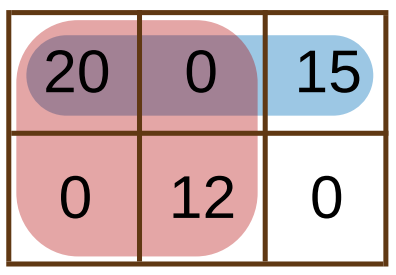
\includegraphics[width=5cm]{ioiruut1.png}% Joonise suurus, joonise fail
    \caption{Ruudustik pärast operatsioone}% Allkiri
    \allikas{IOI 2013}% Allikas
    \label{CPH}% Selle järgi viidatakse, pärast käsku \caption
\end{figure}
Ülemisel pildil on kujutatud ruudustiku pärast eelnevaid operatsioone. Bazza võib seejärel pärida suurimat ühistegurit järgmistes alamruudustikes:
\begin{itemize}
    \item Vastasnurgad on $(0,0)$ ja $(0,2)$: kolm täisarvu selles alamruudustikus on $20$, $0$ ja $15$, ning nende SÜT on $5$.
    \item Vastasnurgad on $(0,0)$ ja $(1,1)$: neli täisarvu selles alamruudustikus on $20$, $0$, $0$ ja $12$,ning nende SÜT on $4$.
\end{itemize}

Nüüd teeb Bazza järgnevad uuendamisoperatsioonid:
\begin{itemize}
    \item Muudab ruudu $(0,1)$ väärtuse $6$-ks.
    \item Muudab ruudu $(1,1)$ väärtuse $14$-ks.
\end{itemize}

\begin{figure}[H]% [] sisse märgitakse paigutus H
    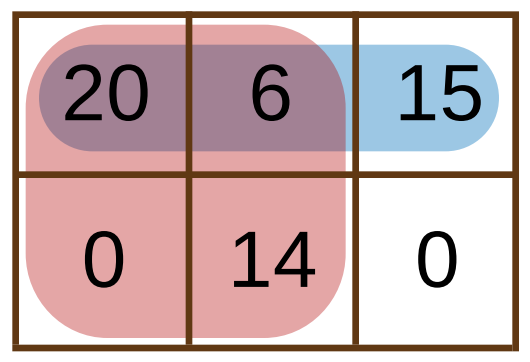
\includegraphics[width=5cm]{ioiruut2.png}% Joonise suurus, joonise fail
    \caption{Ruudustik pärast operatsioone 2}% Allkiri
    \allikas{IOI 2013}% Allikas
    \label{CPH}% Selle järgi viidatakse, pärast käsku \caption
\end{figure}
Ülemisel joonisel on kujutatud ruudustik pärast uuendusi. Bazza võib nüüd pärida SÜT väärtust järgnevates alamruudustikes uuesti:
Vastasnurgad on $(0,0)$ ja $(0,2)$: kolm täisarvu alamruudustikus on $20$, $6$ ja $15$, ning nende SÜT on $1$.
Vastasnurgad on $(0,0)$ ja $(1,1)$: neli täisarvu alamruudustikus on $20$, $6$, $0$ ja $14$, ning nende SÜT on $2$.

Nüüd on Bazza teostanud $N_U=5$ uuendust ja $N_Q$ küsimist.

\textbf{Implementatsiooni juhis}

Sa peaksid esitama faili implementeerides järgmised funktsioonid $init()$ ja $update()$, ning $calculate()$, nagu selgitatud allpool.

On lubatud kasutada kopeeritud SÜT leidmise funktsiooni.

Funktsioon $init()$ peab sisendit võtma kujul:
$void\ init(int\ R,\ int\ C)$, kus $R$ on ridade arv ja $C$ on veergude arv.

Seda funktsiooni kutsutakse ainult programmi initsialiseerimiseks.

Funktsioon $update()$ peab sisendit võtma kujul:
$void\ update(int\ P,\ int\ Q,\ long\ long\ K)$, kus $P$$(0\le P\le R-1)$ on ruudu rida, $Q$$(0\le Q\le C-1)$ on ruudu veerg, ning $K$$(0\le K\le 10^{18})$ on ruudule määratud väärtus.


Funktsioon $calculate()$ peab sisendit võtma kujul:
$long\ long\ calculate(int\ P,\ int\ Q,\ int\ U,\ int\ V)$ , kus $P$$(0\le P\le R-1)$ on alamruudustiku ülemise vasakpoolse nurga rida, $Q$$(0\le Q\le C-1)$ on ülemise vasakpoolse nurga veerg, $U$$(P\le U\le R-1)$ on alumise parempoolse nurga rida, ning $V$$(Q\le V\le C-1)$ on alumise parempoolse nurga veerg.
Lisaks peab see funktsioon tagastama antud alamaruudustiku SÜT, või $0$ juhul kui kõik alamruudustiku ruudud on väärtusega $0$.

\textbf{Alamülesanded}

Iga alamülesande kohta kehtib $0\le K\le 10^{18}$.

\begin{table}[H]
\caption{Alamülesannete piirangud, autori tõlgitud}% Pealkiri
\label{tabel1}% Tabelile viitamine
\begin{tabular}{|l|l|l|l|l|l|l|l|}
\hline
Alamülesanne & Punktid & $R$        & $C$          & $N_U$        & $N_Q$        & Ajalimiit & Mälulimiit \\ \hline
$1$          & $10$    & $\le 100$  & $\le 100$    & $\le 100$    & $\le 100$    & $13$ s    & $230$ MiB  \\ \hline
$2$          & $27$    & $\le 10$   & $\le 100000$ & $\le 250000$ & $\le 250000$ & $13$ s    & $230$ MiB  \\ \hline
$3$          & $26$    & $\le 2000$ & $\le 2000$   & $\le 250000$ & $\le 250000$ & $13$ s    & $230$ MiB  \\ \hline
$4$          & $17$    & $\le 10^9$ & $\le 10^9$   & $\le 250000$ & $\le 250000$ & $13$ s    & $230$ MiB  \\ \hline
$5$          & $20$    & $\le 10^9$ & $\le 10^9$   & $\le 250000$ & $\le 250000$ & $13$ s    & $230$ MiB  \\ \hline
\end{tabular}
\allikas{IOI 2013}% Viide
\end{table}

\textbf{Sisend}

Hindamisprogramm loeb sisendit failist \textbf{game.in}, selle faili formaat peab olema järgnev:
\begin{itemize}
    \item Rida 1: $R\ C\ N$
    \item Järgmised $N$ rida: üks käik rea kohta
\end{itemize}

Iga käik peab olema ühes formaadis allolevatest:
\begin{itemize}
    \item $update(P,Q,K):\ 1\ P\ Q\ K$
    \item $calculate(P,Q,U,V):\ 2\ P\ Q\ U\ V$
\end{itemize}

Enne läbi käidud näide oleks formaadis:
\begin{verbatim}
2 3 9
1 0 0 20
1 0 2 15
1 1 1 12
2 0 0 0 2
2 0 0 1 1
1 0 1 6
1 1 1 14
2 0 0 0 2
2 0 0 1 1
\end{verbatim}

Mis vastab tabelile:

\begin{figure}[H]% [] sisse märgitakse paigutus H
    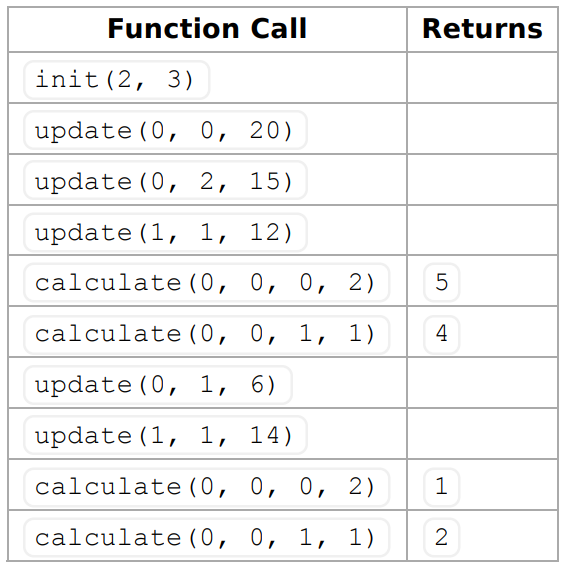
\includegraphics[width=10cm]{ioitabel.png}% Joonise suurus, joonise fail
    \caption{Tabel kus function call tähistab kutsutavat funktsiooni, return tähistab tagastatud väärtust}% Allkiri
    \allikas{IOI 2013}% Allikas
    \label{CPH}% Selle järgi viidatakse, pärast käsku \caption
\end{figure}

\begin{extra}
Ülesande lahendamiseks on kindlasti vaja teha globaalselt:
\begin{cclol}
#include "game.h"
\end{cclol}
\end{extra}

\parencite{IOI}
\end{Text}

\begin{vihje}
Mälu on tõenäoliselt pudelikael.
\end{vihje}

\begin{vihje}
100 punkti lahendusele on omane mälukeerukus $O(Q\log R)$.
\end{vihje}


\begin{solution}
1D variant sellest ülesandest on suhteliselt lihtsasti lahendatav: iga tipp salvesta oma laste SÜT-i(\textbf{kommutatiivne}). Põhjusel, et $R$ võib olla üsna suur, peab see olema hõre lõikude puu; alternatiivina saaks kasutada Fenwicki puud.

2D versioonis võib tunduda ahvatlev kasutada nelikpuud(igal tipul 4 last), kuid see ei taga polülogaritmilist ajakeerukust. 
80 punkti on võimalik kätte saada kasutades vahemikupuud(inglise keeles \textit{range tree}), täispunktide saamiseks on üks variant kasutada 2D hõredat lõikude puud -- optimeerides ajakeerukuse $O(N\log (vahemiku\ suurus))$-lt $O(N)$-ni.

Põhimõtteliselt ei tee me tippe lõikude puus juhul kui need ei ole puu lehed ka hoiavad ainult ühte lehte oma alampuus, sest need tipud on üleliigsed. Selle optimisatsiooni tulemusena saame lõikude puu $N$ lehega $2N-1$ tipuga.

Kasutades seda meetodit veergude lõikude puudel, saame mälukeerukuse $O(Q\log R)$.
Sellest piisab, et saada maksimumpunktid, ning implementatsioon on ka peatüki lõpus kättesaadav.

Kuid leidub veel üks viis, et saada ülesandes täispunktid, selleks on andmestruktuur, mis on põhimõtteliselt lõikude puu vahemikupuudest.
Töös olev näidisimplementatsioon kasutab modifitseeritud puhja(inglise keeles \textit{treap}), kus iga lõikude puu tipp salvestab puhja, ning tipu uuendamine tähendab $O(\log C)$ tipu väärtuse muutmist.

\parencite{IOIS1}\parencite{IOIS2}
\end{solution}

\begin{cclol}
#include "game.h"
#include <stdlib.h>

typedef long long ll;

static int R, C;

struct X_NODE {
X_NODE(int s,int e):s(s),e(e),left(0),right(0),value(0LL){}
	int s, e;
	X_NODE *left, *right;
	ll value;
};

struct Y_NODE {
	Y_NODE() : left(NULL), right(NULL), xtree(1, C) {}
	Y_NODE *left, *right;
	X_NODE xtree;
} *root;

ll gcd2(ll x, ll y) {
	if (y == 0) return x;
	return gcd2(y, x % y);
}

void init(int r, int c) {
	R = r, C = c;
	root = new Y_NODE();
}

void update2(X_NODE *node, int q, ll k) {
	int s = node->s, e = node->e, m = (s + e) >> 1;
	if (s == e) {
		node->value = k;
		return;
	}
	X_NODE **child = &(q <= m ? node->left : node->right);
	if (*child == NULL) {
		*child = new X_NODE(q, q);
		(*child)->value = k;
	} else if ((*child)->s <= q && q <= (*child)->e) {
		update2(*child, q, k);
	} else {
		do {
			if (q <= m) e = m;
			else s = m + 1;
			m = (s + e) >> 1;
		} while ((q <= m) == ((*child)->e <= m));
		X_NODE *nnode = new X_NODE(s, e);
		if ((*child)->e <= m) nnode->left = *child;
		else nnode->right = *child;
		*child = nnode;
		update2(*child, q, k);
	}
	node->value = gcd2(node->left ? node->left->value : 0,
	                   node->right ? node->right->value : 0);
}

ll query2(X_NODE *node, int s, int e) {
	if (node == NULL || node->s > e || node->e < s) return 0;
	if (s <= node->s && node->e <= e) { return node->value; }
return gcd2(query2(node->left,s,e),query2(node->right,s,e));
}

void update1(Y_NODE *node, int s, int e, int p, int q, ll k) {
	int m = (s + e) >> 1;
	if (s == e) {
		update2(&node->xtree, q, k);
		return;
	}
	if (p <= m) {
		if (node->left == NULL) node->left = new Y_NODE();
		update1(node->left, s, m, p, q, k);
	} else {
		if (node->right == NULL) node->right = new Y_NODE();
		update1(node->right, m + 1, e, p, q, k);
	}
	ll v = gcd2(node->left ? query2(&node->left->xtree,q,q):0,
	        node->right ? query2(&node->right->xtree,q,q):0);
	update2(&node->xtree, q, v);
}

void update(int p, int q, ll k) {
	++p, ++q;
	update1(root, 1, R, p, q, k);
}

ll query1(Y_NODE *node, int s, int e, int p, int q, int u, int v) {
	if (node == NULL || s > u || e < p) return 0;
	if (p <= s && e <= u) return query2(&node->xtree, q, v);
	int m = (s + e) >> 1;
	return gcd2(query1(node->left, s, m, p, q, u, v),
	            query1(node->right, m + 1, e, p, q, u, v));
}

ll calculate(int p, int q, int u, int v) {
	++p, ++q, ++u, ++v;
	return query1(root, 1, R, p, q, u, v);
}
\end{cclol}
\begin{kk}[H]
\caption{Implementatsioon ülesandele Game, mis kasutab optimeeritud 2D lõikude puud}% Allkiri
\allikas{Andi Qu vabavara implementatsioon}% Allikas
\end{kk}


\begin{cclol}
#include "game.h"

#include <bits/stdc++.h>
typedef long long ll;
using namespace std;

ll gcd(ll x, ll y) { return !y ? x : gcd(y, x % y); }
int rnd() { return ((rand()%(1 << 15)) << 16)+(rand() % (1 << 15));}

struct TreapNode {
	TreapNode *l, *r;
	int pos, key, mn, mx;
	ll val, g;

	TreapNode(int position, ll value) {
		l = r = nullptr;
		mn = mx = pos = position;
		key = rnd();
		val = g = value;
	}

	void update() {
		g = val;
		if (l) g = gcd(g, l->g);
		if (r) g = gcd(g, r->g);
		mn = (l ? l->mn : pos);
		mx = (r ? r->mx : pos);
	}
};

struct Treap {
	TreapNode *root;

	Treap() {
		root = nullptr;
		srand(rnd());
	}

void split(TreapNode *t,int pos,TreapNode *&l,TreapNode *&r){
		if (t == nullptr) {
			l = r = nullptr;
			return;
		}
		if (t->pos < pos) {
			split(t->r, pos, l, r);
			t->r = l;
			l = t;
		} else {
			split(t->l, pos, l, r);
			t->l = r;
			r = t;
		}
		t->update();
	}

	TreapNode *merge(TreapNode *l, TreapNode *r) {
		if (!l || !r) return l ? l : r;
		if (l->key < r->key) {
			l->r = merge(l->r, r);
			l->update();
			return l;
		} else {
			r->l = merge(l, r->l);
			r->update();
			return r;
		}
	}

	bool find(int pos) {
		TreapNode *t = root;
		while (t) {
			if (t->pos == pos) return true;
			if (t->pos > pos) t = t->l;
			else t = t->r;
		}
		return false;
	}

	void update(TreapNode *t, int pos, ll val) {
		if (t->pos == pos) {
			t->val = val;
			t->update();
			return;
		}
		if (t->pos > pos) update(t->l, pos, val);
		else update(t->r, pos, val);
		t->update();
	}

	void insert(int pos, ll val) {
		if (find(pos)) update(root, pos, val);
		else {
			TreapNode *l, *r;
			split(root, pos, l, r);
	root = merge(merge(l, new TreapNode(pos, val)), r);
		}
	}

	ll query(TreapNode *t, int st, int en) {
		if (t->mx < st || en < t->mn) return 0;
		if (st <= t->mn && t->mx <= en) return t->g;

		ll ans = (st <= t->pos && t->pos <= en ? t->val : 0);
		if (t->l) ans = gcd(ans, query(t->l, st, en));
		if (t->r) ans = gcd(ans, query(t->r, st, en));
		return ans;
	}
	ll query(int st, int en) {
		if (!root) return 0;
		return query(root, st, en);
	}
};

struct Segtree {
	Segtree *l, *r;
	Treap treap;
	int lo, hi;

	Segtree() { l = r = nullptr; }
	Segtree(int st, int en) {
		l = r = nullptr;
		lo = st, hi = en;
	}

	void new_left() {
		if (!l) l = new Segtree(lo, (lo + hi) / 2);
	}
	void new_right() {
		if (!r) r = new Segtree((lo + hi) / 2 + 1, hi);
	}
	void fix(int pos) {
		ll val = 0;
		if (l) val = gcd(val, l->treap.query(pos, pos));
		if (r) val = gcd(val, r->treap.query(pos, pos));
		treap.insert(pos, val);
	}

	void update(int x, int y, ll val) {
		if (hi < x || x < lo) return;
		if (lo == hi) {
			treap.insert(y, val);
			return;
		}

		if (x <= (lo + hi) / 2) {
			new_left();
			l->update(x, y, val);
		} else {
			new_right();
			r->update(x, y, val);
		}
		fix(y);
	}

	ll query(int t, int b, int st, int en) {
		if (hi < t || b < lo) return 0;
		if (t <= lo && hi <= b) return treap.query(st, en);

		ll ans = 0;
		if (l) ans = gcd(ans, l->query(t, b, st, en));
		if (r) ans = gcd(ans, r->query(t, b, st, en));
		return ans;
	}
};

Segtree segtree;

void init(int R, int C) {
	srand(12341234);
	segtree = Segtree(0, R - 1);
}

void update(int P, int Q, ll K) { segtree.update(P, Q, K); }

ll calculate(int P,int Q,int U,int V){return segtree.query(P,U,Q,V);}
\end{cclol}
\begin{kk}[H]
\caption{Implementatsioon ülesandele Game, mis kasutab optimeeritud lõikude puud Fenwicki puudest}% Allkiri
\allikas{Andi Qu vabavara implementatsioon}% Allikas
\end{kk}

\subsection{Ülesanded lisateemadele}
Nimekiri ülesannetest mille temaatika läheb natuke uurimistöö omast välja, kuid mis siiski on väga tugevalt seotud lõikude puu teooriaga, põhjusel, et mõlemad teevad päringuid lõikudel efektiivsemaks.
Eriti kasulikuks on osutunud andmestruktuur indekseeritud hulk(vt Lisa 13), mis on üllatavalt vähetuntud arvestades selle kasulikkust. Autor ei olnud teadlik andmestruktuurist enne töö koostamist, ning tutvus selle funktsionaalsusega töö käigus.


\subsubsection{Prefiksi summaga lahendatavad ülesanded}
Selles peatükis leidub selgitusi erinevatele prefiksi summa võttega lahendatavale ülesannetele, ning mainitakse ka vahepeal miks ei sobi käsitletud juhtudel lõikude puuga lahendus.
\begin{prereq}
Prefiksi summad(Lisa 11)
\end{prereq}
\paragraph{Subarray Divisibility, CSES, *}
\begin{extra}
Ülesannet saab esitada \href{https://cses.fi/problemset/task/1662}{CSES platvormil}.
\end{extra}
\begin{prereq}
Prefiksi summa leidmine(vt Lisa 11), jaguvus, alamhulga mõiste
\end{prereq}
\begin{Text}
Sisendine antakse $n$ täisarvu, ülesandeks on leida alamhulkade arv mille väärtuste summa jagub $n$-ga.

\parencite{div}
\end{Text}
\begin{Input}
Esimesel real on täisarv $n$: massiivi suurus.

Teisel real on $n$$(1\le n\le 2\cdot 10^5)$ täisarvu $a_1,a_2,...,a_n$$(-10^9\le a_i\le 10^9)$: massiivi elementide väärtused.
\end{Input}
\begin{Output}
Väljasta üks täisarv: omadusele vastavata alamhulkade arv.
\end{Output}

\textbf{Näidissisend}

\begin{verbatim}
5
3 1 2 7 4
\end{verbatim}

\textbf{Näidisväljund}

\begin{verbatim}
1
\end{verbatim}


\begin{vihje}
Lahenduse ajakeerukus on $O(n)$.
\end{vihje}


\begin{solution}
Peame leidam alamhulkade arvu mis jaguvad $N$-ga, teisisõnu peame leidma alamhulkade arvu mille summa on $0\ (mod\ N)$.

Kusjuures, iga alamhulga summat saab käsitleda kahe prefiksi vahena. 

Ütleme, et $sum$ on massiivi $a$ prefiksi summa $mod\ N$.

Teame, et:
\[sum(i,j)=sum(0,j)-sum(0,i-1)\]
Seepärast, et tahame leida $sum(i, j)$ hulka mis on võrdne $0\ (mod\ N)$, peab $sum(0,j)$ olema võrdne $sum(0,i-1)$, et nende vahe oleks 0.

Nüüd arvutame $pmod[i]$ -- prefiksite arv mis on võrdne jäägiga $i\ (mod\ N)$. Siis $i$ lisab paare:

$$
{\texttt{pmod}[i]\choose{2}} = \texttt{pmod}[i] \cdot (\texttt{pmod}[i] - 1) / 2
$$

Vastus on selle hulga summa iga $i$ kohta.
\end{solution}

Järgnev on autori implementatsioon:
\begin{cclol}
#include <bits/stdc++.h>

using namespace std;

#define ll long long

#pragma GCC optimize("O3,unroll-loops")
#pragma GCC target("avx2,bmi,bmi2,popcnt,lzcnt")

int main(int argc, char ** argv) {
  ios_base::sync_with_stdio(false);
  cin.tie(NULL);
  int n;
  cin >> n;
  ll num;
  ll preSum = 0;
  unordered_map < ll, int > m;
  m[0] = 1;
  ll ans = 0;
  for (int i = 0; i < n; i++) {
    cin >> num;
    preSum = (preSum + num) % n;
    if (preSum < 0) {
      preSum += n;
    }
    ans += m[preSum];
    m[preSum]++;
  }

  cout << ans;
  return 0;
}
}
\end{cclol}
\begin{kk}[H]
\caption{Implementatsioon ülesandele Subarray Divisibility}% Allkiri
\allikas{Autori implementatsioon}% Allikas
\end{kk}

\paragraph{Subarray Sums II, CSES, *}
\begin{extra}
Ülesannet saab esitada \href{https://cses.fi/problemset/task/1661}{CSES platvormil}.
\end{extra}
\begin{prereq}
Prefiksi summa leidmine(vt Lisa 11)
\end{prereq}
\begin{Text}
Sisendina antakse suurusega $n$ massiiv , peame leidma mitmel alamhulgal on summa $x$.

\parencite{sums}
\end{Text}
\begin{Input}
Esimesel real on kaks täisarvu $n$$(1\le n\le 2\cdot 10^5)$ ja $x$: massiivi suurus ja soovitud summa $x$$(-10^9\le x,a_i\le 10^9)$.

Teisel real on $n$ täisarvu $a_1,a_2,...,a_n$: massiivi elementide väärtused.
\end{Input}
\begin{Output}
Väljasta üks täisarv: omadusele vastavate alamhulkade arv.
\end{Output}

\textbf{Näidissisend}

\begin{verbatim}
5 7
2 -1 3 5 -2
\end{verbatim}

\textbf{Näidisväljund}

\begin{verbatim}
2
\end{verbatim}

\begin{solution}
Saame kasutada assotsiatiivset konteinerit, näiteks std::map, mis hoiab prefiksi summasid. Iga index $i$ kohta, saame leida prefiksiti arvu mille summa on võrdne $prefiksiSumma[i]-x$. Selle abil saame eemaldada prefiksi meie praegusest prefiksist, et ehitada alamhulk summaga $x$. Peale igat iteratsiooni lisame uue prefiksi summa konteinerisse.
\end{solution}


\begin{cclol}
#include <bits/stdc++.h>

using namespace std;

#define ll long long

#pragma GCC optimize("O3,unroll-loops")
#pragma GCC target("avx2,bmi,bmi2,popcnt,lzcnt")

int main(int argc, char ** argv) {
  ios_base::sync_with_stdio(false);
  cin.tie(NULL);
  int n, x;
  cin >> n >> x;
  ll num;
  ll preSum = 0;
  unordered_map < ll, int > m;
  m[0] = 1;
  ll ans = 0;
  for (int i = 0; i < n; i++) {
    cin >> num;
    preSum += num;
    ans += m[preSum - x];
    m[preSum]++;
  }

  cout << ans;
  return 0;
}
\end{cclol}
\begin{kk}[H]
\caption{Implementatsioon}% Allkiri
\allikas{Autori implementatsioon}% Allikas
\end{kk}

\paragraph{Forest Queries, CSES, **}
\begin{extra}
Ülesannet saab esitada \href{https://cses.fi/problemset/task/1652}{CSES platvormil}.
\end{extra}
\begin{prereq}
2D prefiksi summa võte(vt Lisa 12)
\end{prereq}
\begin{Text}
Antakse $n$ x $n$ ruudustik kujutamaks kaarti metsamaastikust. Iga ruut on kas tühi või sisaldab puud. Ülapoolsel vasakul nurgal on koordinaadid $(1, 1)$, ning vastasnurga ruudul on koordinaadid $(n, n)$.

Ülesandeks on täita $q$ päringut kujul -- kui palju puid on antud alamruudustiku sees kaardil?

\parencite{forest}
\end{Text}
\begin{Input}
Esimesel real on kaks täisarvu $n$ ja $q$$(1\le n\le 1000, 1\le q\le 2\cdot 10^5)$: kaardi suurus ja päringute arv.

Seejärel antakse sisendina $n$ rida, millest igaühel on $n$ kirjamärki, kus . on tühi ruut ja * on puu.

Sellele järgnevad $q$ rida päringuid. Igal real on neli täisarvu $y_1, x_1, y_2, x_2$$(1\le y_1\le y_2\le n; 1\le x_1\le x_2\le n)$, mis tähistavad alamruudustiku nurga koordinaate.

\end{Input}

\begin{Output}
Väljasta puude arv iga antud alamruudustiku sees.
\end{Output}



\textbf{Näidissisend}

\begin{verbatim}
4 3
.*..
*.**
**..
****
2 2 3 4
3 1 3 1
1 1 2 2
\end{verbatim}

\textbf{Näidisväljund}

\begin{verbatim}
3
1
2
\end{verbatim}


\begin{vihje}
Tegu on üsnagi standardse ülesandega, mille lahendamiseks pead lihtsalt oskama 2D prefiksi summa võtet.
\end{vihje}

\begin{solution}
Kood vastab valemile:
$$
\begin{aligned}
\sum_{i=a}^{A} \sum_{j=b}^{B} \texttt{arr}[i][j]=&\,\texttt{prefix}[A][B]
		- \texttt{prefix}[a-1][B] \\
		&- \texttt{prefix}[A][b-1] + \texttt{prefix}[a-1][b-1]
\end{aligned}
$$
Kus $a$ ja $A$ on alammaatriksi vasakpoolseim ja parempoolseim rida, ning $b$ ja $B$ veerud vastavalt samamoodi.
\end{solution}
\begin{cclol}
#include <bits/stdc++.h>

using namespace std;

#pragma GCC optimize("O3,unroll-loops")
#pragma GCC target("avx2,bmi,bmi2,popcnt,lzcnt")

int main(int argc, char ** argv) {
  ios_base::sync_with_stdio(false);
  cin.tie(NULL);
  int n;
  cin >> n;
  int arr[n + 1][n + 1];
  memset(arr, 0, sizeof(arr));
  int q;
  cin >> q;
  char temp;
  for (int i = 1; i < n + 1; i++) {
    for (int j = 1; j < n + 1; j++) {
      cin >> temp;
      if (temp == '*') arr[i][j]++;
    }
  }
  for (int i = 1; i < n + 1; i++) {
    partial_sum(arr[i], arr[i] + n + 1, arr[i]);
  }

  for (int i = 1; i < n + 1; i++) {
    int tot = 0;
    for (int j = 1; j < n + 1; j++) {
      tot += arr[j][i];
      arr[j][i] = tot;
    }
  }

  int a, b, c, d;
  for (int i = 0; i < q; i++) {
    cin >> a >> b >> c >> d;
cout << arr[c][d]-arr[a-1][d]-arr[c][b-1]+arr[a-1][b-1] << endl;
  }

  return 0;
}
\end{cclol}
\begin{kk}[H]
\caption{Implementatsioon}% Allkiri
\allikas{Autori implementatsioon}% Allikas
\end{kk}

\paragraph{Multiple of 2019, AtCoder, ***}
\begin{extra}
Ülesannet saab esitada \href{https://atcoder.jp/contests/abc164/tasks/abc164_d}{AtCoder platvormil}.
\end{extra}
\begin{prereq}
Prefiksu summa võte(vt Lisa 11), modulaararitmeetika(vt Lisa 10)
\end{prereq}
\begin{Text}
Sisendina antakse sõne $S$, mis koosneb arvudest $1$ kuni $9$.
Vaja on leida paaride arv$(i,j)$$(1\le i\le j\le |S|)$, millel on omadus:
\begin{itemize}
    \item Kümnendsüsteemis, tähemärgid sõnes $S$ vahemikus $i$ kuni $j$  moodustavad summa mis jagub $2019$-ga.
\end{itemize}

\parencite{16}
\end{Text}

\begin{Input}
$S$
\end{Input}

\begin{Output}
Väljasta paaride arv$(i,j)$$(1\le i\le j\le |S|)$, mis vastavad eelnevale omadusele.
\end{Output}

\textbf{Näidissisend 1}

\begin{verbatim}
1817181712114
\end{verbatim}

\textbf{Näidisväljund 1}

\begin{verbatim}
3
\end{verbatim}





\textbf{Näidissisend 2}

\begin{verbatim}
14282668646
\end{verbatim}

\textbf{Näidisväljund 2}

\begin{verbatim}
2
\end{verbatim}


\begin{extra}
Väga soliidne selgitus ülesande lahenduskäigust on kättesaadaval YouTube kanalil Errichto.
\end{extra}
\begin{solution}
Et salvestada sõne lõike, saame teha suffiksi massiivi $S$, kujul:
$${S_i = s_n + 10*s_{n-1} +100*s_{n-2} + ... + {10^{n-i}} \cdot s_{i}}$$

Näiteks, kui meie sõne oleks $1234$ ja $mod$ oleks $3$($2019$ asemel), oleks suffiksi massiiv:

$$[1234, 234, 34, 4, 0]$$

Arvestatakse ka tühja suffiksit.

See on kasulik põhjusel, et saame iga alamsõne $O(1)$ ajakeerukusega.
Ehk siis kui ${S_0} = 1234$ ja  ${S_3=4}$, s.t ${S_0}-{S_3} = 123 \cdot {10^1}$ või $1230$.

Samuti tähendab eelnev, et kui mõlemad ${S_0}(mod$ $M)=$ ${S_3}(mod$ $M)$(mõlemal suffiksil on samad jäägid), lahutades saame ${S_0}(mod$ $M)-$ ${S_3}(mod$ $M)=0$, mis omakorda tähendaks, et alamsõne jaguks $2019$-ga.

Ehk siis $1234$, ${S_0-{S_3}=1234(mod}$ $3)-4(mod$ $3)=1-1=0$. Seepärast, et lahutamisel saab nendest $0$, on alamsõne indeksist $0$ kuni $2$ arv, mis jagub antud $mod$-ga(näiteks $123$ jagub $3$-ga). 

Kuid peaksime ikkagi käime läbi iga paari võimalikke suffikseid $(i, j)$, mis tähendaks ajakeerukust $O(N^2)$. 
Aga me ei peagi teadma millisel suffiksil on mingi kindel jääk vaid hoopis kui paljudel suffiksitel on mingi kindel jääk.
Saame võtta ${N \choose K}$, ning valida kaks numbrit mis jaguvad same jäägiga $2019$, kus $N=$ mitu korda mingi jääk tekib, ehk $K=$ 2 (sest me valime kaks indeksit $i$ ja $j$).

Sellest saame järeldada, et vastus on kõikide jääkide hulk $0...2018$ massiivis ja ${N \choose 2}$.

Meie näites $1234$, näeks meie uus massiiv välja järgnevalt:

$[2, 3, 0]$

Kus iga index tähistab mingi jäägi hulka:
\begin{itemize}
\item Meil on $2$ suffiksit jäägiga $0$ kui jagada $3$, $[234, 0]$.
\item Saame $3$ suffiksit jäägiga $1$ kui jagada $3$, $[1234, 34, 4]$.
\item Ning meil ei ole suffikseid jäägiga $2$.
\end{itemize}

Saame, et nende kõikide arvude summa oleks ${2 \choose 2} + {3 \choose 2}=1+3=4$.

Juhul kui $N<K$, oleks see $0$, sest seal ei ole piisavalt suffikseid mis saaksid moodustada paari.

\end{solution}

\begin{cclol}
#include <bits/stdc++.h>

using namespace std;

#define ll long long

#pragma GCC optimize("O3,unroll-loops")
#pragma GCC target("avx2,bmi,bmi2,popcnt,lzcnt")

int main(int argc, char ** argv) {
  ios_base::sync_with_stdio(false);
  cin.tie(NULL);
  string s;
  cin >> s;
  int n = s.length();
  map < ll, int > m;
  ll pow = 1;
  ll num = 0;
  ll ans = 0;
  m[0] = 1;
  for (int i = n - 1; i >= 0; i--) {
    num = (num + (s[i] - '0') * pow) % 2019;
    pow = (pow * 10) % 2019;
    ans += m[num];
    m[num]++;
  }

  cout << ans;

  return 0;
}
\end{cclol}
\begin{kk}[H]
\caption{Implementatsioon}% Allkiri
\allikas{Autori implementatsioon}% Allikas
\end{kk}



\paragraph{Cow Hopscotch, USACO Gold lahtine võistlus 2010, *****}
\begin{extra}
Ülesanne on nii vana, et kahjuks seda esitada ei saa, kuid testid on kättesaadavad \href{https://codeforces.com/blog/entry/95032}{Codeforces blogis}.
\end{extra}
%\begin{extra}
%See ülesanne on nn Old Gold ülesanne, mis tähendab, et pärineb ajast kui USA informaatkaolümpiaadil veel ei olnud Platinum järku. Sellest tuleneb ka see, et ülesanne on Gold järku ülesande kohta ebatavaliselt raske.
%\end{extra}

\begin{Text}
Lehmad on nostalgilised lapsepõlve üle, ning otsustasid hakata mängima ka neile tuntud keksu. Nende mängus on rida $N$($3\le N\le 250000$) ruutudest, nummerdatud $1..N$.

Nagu iga hea mäng, on nende keksumängus auhinnad! Ruut $i$ on rahalise väärtusega $V_i$($-2\cdot 10^9\le V_i\le 2\cdot 10^9$). Lehmad tahavad teada kes suudab kõige rohkem raha teenida.

Reeglid on suhteliselt lihtsad:
\begin{itemize}
    \item Iga lehm alustab ruudul $0$, sellel ruudul puudub rahaline väärtus.
    \item Seejärel teeb lehm mingi hulga hüppeid ruudu $N$ poole(võib ka teha $0$ hüpet). Iga ruut mille peale ta langeb saab olla maksimaalselt $K$($2\le K\le N$) ruudu kaugusel eelnevast ruudust.
    \item Kui lehm soovib, sis võib ta ka pöörata ümber ja liikuda ükshaaval tagasi ruudu $0$ peale.
    \item Lehm kuigi ei tohi maanduda ühegi ruudu peale, kus ta on juba varem olnud liikudes $0$-st kaugemale.
    \item Peale ruudu $0$, peavad ruudud millele ta maandub tagasiteel eelnema ruutudele millele ta juba maandus $0$-st kaugenedes.
\end{itemize}

Lehm teenib raha niipalju kui on nende ruutude summa mille peale ta hüppas. Väljasta suurim rahasumma mida on lehmal võimalik teenida.

Ütleme, et meil on selline ruudurada, kus $K$ väärtus on $3$:
\begin{verbatim}
Ruudu num.:    0      1      2      3      4      5      6
             +---+  +---+  +---+  +---+  +---+  +---+  +---+
             |///|--|   |--|   |--|   |--|   |--|   |--|   |
             +---+  +---+  +---+  +---+  +---+  +---+  +---+
     Väär.:    -      0      1      2     -3      4      5
\end{verbatim}
Üks optimaalne viis lehmal hüpata oleks näiteks: $1[0], 3[2], 6[5], 5[4], 2[1], 0[0]$, raha teeniks lehm siis -- $0+2+5+4+1+0=12$.

Kui lehm hüppaks alguses näiteks: $0, 1, 2, 3, 4, ...$, siis tekiks olukord kus oleks võimatu lehmal leida tagasiteed, sest ei ole lubatud tagasiteel maanduda puutumata ruudule.

\parencite{18}
\end{Text}
\begin{Input}
Täisarvud $N$ ja $K$.
$2..N+1$ rida($i+1$) milles igaühel on üks täisarv $V_i$.
\end{Input}
\begin{Output}
Väljasta üks täisarv -- maksimaalne rahasumma mida on võimalik lehmal teenida.
\end{Output}



\textbf{Näidissisend}

\begin{verbatim}
6 3
0
1
2
-3
4
5
\end{verbatim}

\textbf{Näidisväljund}

\begin{verbatim}
12
\end{verbatim}


\begin{vihje}
Dünaamiline planeerimine.
\end{vihje}

\begin{solution}
Ülesande lahenduse dünaamilise planeerimise abil vastab valemile:
\[dp[i] = dp[j] + V[i] + V[i-1] + PrefiksiSumma[i-2] - PrefiksiSumma[j]\]
Iga $i-1-k \le j < i-1$ kohta.

Optimiseerida $O(N)$ keerukuseni saab max queue abil, pannes kõik $j$ väärtust ($dp[j]-PrefiksiSumma[j]$) max queue sisse.

Koodi lugemine teeb tõenäoliselt algoritmi arusaadavamaks.
\end{solution}
\begin{cclol}
#include <bits/stdc++.h>

using namespace std;

int N, K;
vector < long long > dp;
vector < long long > V;

struct maxqueue {
  deque < pair < long long, int >> dq;

  void insert_back(pair < long long, int > val) {
    while (!dq.empty() && dq.back().first <= val.first) {
      dq.pop_back();
    }
    dq.push_back(val);
  }
  void delete_front(int ind) {
    while (!dq.empty() && dq.front().second < ind) {
      dq.pop_front();
    }
  }
  long long get_max() {
    if (!dq.empty()) {
      return dq.front().first;
    } else {
      // change this
      return -1;
    }
  }
};

int main() {
  // sliding window of previous dp states
  // go from i to j?
  // ifstream cin("hop.in");

  cin >> N >> K;
  V.resize(N + 1);
  dp.resize(N + 1);
  for (int i = 1; i <= N; i++) {
    cin >> V[i];
  }

  vector < long long > nums(N + 1);
  for (int i = 1; i <= N; i++) {
    nums[i] = max(nums[i - 1], nums[i - 1] + V[i]);
  }

  // dp[j] = best solution for first j squares

  dp[1] = max(dp[0], V[1]);
  maxqueue maxQ;

  // go from i to j
  for (int i = 2; i <= N; i++) {
    // update dq
    maxQ.delete_front(i - K);
    // can only be i - 2, as i - 1 is used in dp[i]
    maxQ.insert_back({
      dp[i - 2] - nums[i - 2],
      i - 2
    });

    dp[i] = maxQ.get_max() + V[i] + V[i - 1] + nums[i - 2];
  }

  long long ans = 0;
  for (int i = 1; i <= N; i++) {
    ans = max(ans, dp[i] + nums[min(i - 1 + K, N)] - nums[i]);
  }
  cout << ans;
}
\end{cclol}
 \begin{kk}[H]% [] sisse märgitakse paigutus H
    \caption{Lahenduse implementatsioon ülesandele Cow Hopscotch}% Allkiri
    \allikas{Starcoder}% Allikas
    \label{EMaxx}% Selle järgi viidatakse, pärast käsku \caption
    \end{kk}
    
\subsubsection{Indekseeritud hulgaga lahendatavad ülesanded}
Siin on nimekiri sellistest ülesannetest mida on võimalik lahendada ka lõikude puuga ja fenwicki puuga, kuid indekseeritud hulgaga on see oluliselt lihtsam.
Rohkem infot andmestruktuuri kohta on lisas number 13.
See tähendab muidugi ka, et siin peatükis kehtib iga ülesande kohta:
\begin{prereq}
Indekseeritud hulk
\end{prereq}


\paragraph{List Removals, CSES, *}
\begin{extra}
Ülesannet saab esitada \href{https://cses.fi/problemset/task/1749}{CSES platvormil}.
\end{extra}
\begin{Text}
Sisendine antakse $n$ täisarvust koosnev massiiv. Vaja on eemaldada elemendid antud positsioonidel, ning tagastada eemaldatud elemendi väärtus.

\parencite{list}
\end{Text}
\begin{Input}
Esimesel real on täisarv $n$$(1\le n\le 2\cdot 10^5)$: masiivi suurus. Elemendid on nummerdatud $1,2,...,k$, kus $k$ on hetkel massiivi suurus.

Teisel real on $n$ täisarvu $x_1,x_2,...x_n$$(1\le x_i\le 10^9)$: elementide väärtused.

Viimasel real on $n$ täisarvu $p_1,p_2,...,p_n$$(1\le p_i\le n-i+1)$: eemaldavate elementide asukohad.
\end{Input}
\begin{Output}
Väljasta elemendid järjekorras milles need eemaldatakse.
\end{Output}


\textbf{Näidissisend}

\begin{verbatim}
5
2 6 1 4 2
3 1 3 1 1
\end{verbatim}

\textbf{Näidisväljund}

\begin{verbatim}
1 2 2 6 4
\end{verbatim}
\begin{extra}
Näidisväljundis on listi elemendid: $[2,6,1,4,2], [2,6,4,2], [6,4,2], [6,4], [4]$
 ja $[]$.
\end{extra}

\begin{solution}
$n$ on maksimaalselt $2\cdot 10^5$, sellest saab järeldada, et sobiksid ajakeerukused alates $O(N\log N)$ allapoole.
Algul võib tunduda, et ülesannet saab lahendada tavapärase massiiviga(nt std::array), kuid see ei sobi, sest massiivi suurus võib muutuda, ehk elemendid nihkuvad.

Pidades kõike eelnevat silmas peaks nüüd olema märgata, et ülesande lahendamiseks sobib ideaalselt indekseeritud hulk.
Sellepärast, et soovime hoida iga elemendi kohta kahte täisarvu, see on, indeksit ja väärtust, kasutame pair'i.
\end{solution}
\begin{cclol}    
#include <bits/stdc++.h>

using namespace std;

#pragma GCC optimize("O3,unroll-loops")
#pragma GCC target("avx2,bmi,bmi2,popcnt,lzcnt")

#define pii pair < int, int >

  #include <ext/pb_ds/assoc_container.hpp>

  using namespace __gnu_pbds;

typedef tree < pii, null_type, less < pii > , rb_tree_tag, 
tree_order_statistics_node_update > inset;

int main() {
  ios_base::sync_with_stdio(false);
  cin.tie(NULL);
  int n;
  cin >> n;
  inset tt;
  for (int i = 0; i < n; i++) {
    int x;
    cin >> x;
    tt.insert({
      i,
      x
    });
  }

  for (int i = 0; i < n; i++) {
    int j;
    cin >> j;
    j--;
    auto itr = tt.find_by_order(j);
    cout << ( * itr).second << " ";
    tt.erase(itr);
  }

  return 0;
}
    \end{cclol}
    \begin{kk}[H]
    \caption{CSES List Removals}% Allkiri
    \allikas{Autori implementatsioon}% Allikas
    \end{kk}

\paragraph{Inversions, Codeforces EDU, *}
\begin{extra}
Ülesannet saab esitada \href{https://codeforces.com/edu/course/2/lesson/4/3/practice/contest/274545/problem/A}{Codeforces platvormi EDU lehel}.
\end{extra}
\begin{Text}
Sisendina antakse permutatsioon $p_i$ mis koosneb $n$ elemendist, leidma peab iga $i$ kohta mitu $j$
on sellist, et $j<i$ ja $p_j > p_i$.

\parencite{24}
\end{Text}
\begin{Input}
Esimesel real on $n$$(1\le n\le 10^5)$, teisel real on $n$ täisarvu $p_i$.
On garanteeritud, et $p_i$ moodustab permutatsiooni numbridest $1..n$.
\end{Input}
\begin{Output}
Väljasta $n$ täisarvu, kus $i$-ndas arv on võrdne $j$ arvule, kus $j<i$ ja $p_j>p_i$.
\end{Output}

\textbf{Näidissisend}

\begin{verbatim}
5
4 1 3 5 2
\end{verbatim}

\textbf{Näidisväljund}

\begin{verbatim}
0 1 1 0 3 
\end{verbatim}


\begin{solution}
Järgnev on visualisatsioon ideest:
\begin{figure}[H]% [] sisse märgitakse paigutus H
    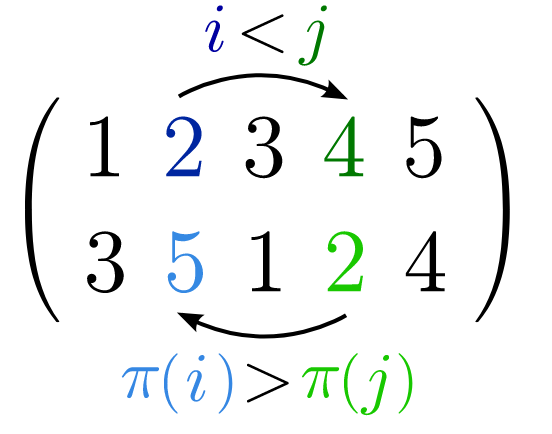
\includegraphics[width=9cm]{inverso.png}% Joonise suurus, joonise fail
    \caption{Inversioonid}% Graafi struktuur
    \allikas{Wikipedia. Inversions(computer science)}% Allikas
    \label{graaf}% Selle järgi viidatakse, pärast käsku \caption
    \end{figure}
Ülesannet saab lahendada sisendi võtmise käigus, ehk võttes sisse elemendi $x$ saame kohe kontrollida, kui palju erineb elemendi asukoht(indeks for tsüklis) elemendi asukohast indekseeritud hulgas -- see ongi inversioonide arv ühe elemendi kohta.
\end{solution}
\begin{cclol}
#include <bits/stdc++.h>

using namespace std;

#pragma GCC optimize("O3,unroll-loops")
#pragma GCC target("avx2,bmi,bmi2,popcnt,lzcnt")

#include <ext/pb_ds/assoc_container.hpp>

using namespace __gnu_pbds;
typedef tree < int, null_type, less < int > , rb_tree_tag, 
tree_order_statistics_node_update > inset;

int main(int argc, char ** argv) {
  ios_base::sync_with_stdio(false);
  cin.tie(NULL);
  int n;
  cin >> n;
  inset tt;

  for (int i = 0; i < n; i++) {
    int x;
    cin >> x;
    cout << i - tt.order_of_key(x) << " ";

    tt.insert(x);
  }

  return 0;
}
    \end{cclol}
    \begin{kk}[H]
    \caption{Codeforces, Inversions}% Allkiri
    \allikas{Autori implementatsioon}% Allikas
    \end{kk}

\paragraph{Salary Queries, CSES, **}
\begin{extra}
Ülesannet saab esitada \href{https://cses.fi/problemset/task/1144}{CSES platvormil}.
\end{extra}
\begin{Text}
Firmal on $n$ palgatud töötajat. Ülesandeks on pidada meeles palku ja vastata päringutele.

\parencite{salary}
\end{Text}
\begin{Input}
Esimesel real on kaks täisarvu $n$ ja $q$$(1\le n, q\le 2\cdot 10^5)$: töötajate arv ja päringute arv.
Töötajad on indekseeritud $1,2,...,n$.

Teisel real on $n$ täisarvu $p_1,p_2,...,p_n$$(1\le p_i\le 10^9)$: töötajate palgad.

   Sellele järgneb $q$ päringut kujul:
\begin{itemize}
\item $!$ $k$ $x$: muuda elemendi $k$$(1\le k\le n)$ väärtus $x$-ks$(1\le x\le 10^9)$.
\item $?$ $a$ $b$ : leia elementide hulk mille väärtus on vahemikus $a…b$$(1\le a\le b\le 10^9)$.
\end{itemize}
\end{Input}
\begin{Output}
Väljasta vastus iga $?$ tüüpi päringule.
\end{Output}

\textbf{Näidissisend}

\begin{verbatim}
5 3
3 7 2 2 5
? 2 3
! 3 6
? 2 3
\end{verbatim}

\textbf{Näidisväljund}

\begin{verbatim}
3
2
\end{verbatim}


\begin{solution}
Sellest ülesandest võib mõelda kui natuke keerulisemast variatsioonist eelmisest ülesandest.

Esiteks, kui kasutada lahenduses indekseeritud hulka, on meil vaja kasutada teist lisas 10 tutvustatud funktsiooni nimetusega $order\_of\_key()$.

Täpsemalt kasutame order of key funktsiooni et täita teist tüüpi päringut, mille toetamiseks, kasutame pair'e.

Esimese päringutüübi täitmiseks kustutame lihtsalt aegunud elemendi, ning lisame hulka uuendatud elemendi, ehk praegusel juhul kustutame $k$ eelmise väärtusega, lisame $k$ väärtusega $x$.
\end{solution}
\begin{cclol}
#include <bits/stdc++.h>

using namespace std;

#define cint
const int
#define pii pair < int, int >

#pragma GCC optimize("O3,unroll-loops")
#pragma GCC target("avx2,bmi,bmi2,popcnt,lzcnt")

cint MM = 1e9 + 7;

#include <ext/pb_ds/assoc_container.hpp>

using namespace __gnu_pbds;

typedef tree < pii, null_type, less < pii > , rb_tree_tag, 
tree_order_statistics_node_update > inset;

int main() {
  ios_base::sync_with_stdio(false);
  cin.tie(NULL);
  int n, q;
  cin >> n >> q;
  inset tt;
  vector < int > v(n);
  for (int i = 0; i < n; i++) {
    cin >> v[i];
    tt.insert({
      v[i],
      i
    });
  }
  for (int i = 0; i < q; i++) {
    char type;
    cin >> type;
    if (type == '!') {
      int x, val;
      cin >> x >> val;
      x--;
      tt.erase({
        v[x],
        x
      });
      v[x] = val;
      tt.insert({
        v[x],
        x
      });
    } else {
      int l, r;
      cin >> l >> r;
      int ans = tt.order_of_key({
        r,
        MM
      }) - tt.order_of_key({
        l,
        -MM
      });
      cout << ans << endl;
    }
  }

  return 0;
}
    \end{cclol}
    \begin{kk}[H]
    \caption{CSES, Salary Queries}% Allkiri
    \allikas{Autori implementatsioon}% Allikas
    \end{kk}
\paragraph{Mega Inversions, Kattis, ***}
\begin{extra}
Ülesannet saab esitada \href{https://open.kattis.com/problems/megainversions}{Kattis platvormil}.
\end{extra}
\begin{prereq}
Inversiooni mõiste
\end{prereq}
\begin{Text}
$n^2$ ülempiiri sorteerimisalgoritmidele on lihtne tuletada: lihtsalt võta kaks elementi, mis on üksteise suhtes valesti paigutatud ja vaheta nende asukohad.
Konrad leiutas algoritmi, mis ei võta mitte kaks valesti paigutatud elementi vaid hoopis kolm. See tähendab, võtab kolm elementi $a_i>a_j>a_k$ kus $i>j>k$ ja paigutab nad järjekorda $a_k, a_j, a_i$. Nüüd kui algses algoritmis oli sammude ülempiiriks maksimaalse inversioonide arvuga $\frac{n(n-1)}{2}$, Konrad on tõelises tupikus, sest ta ei suuda välja nuputada mis võiks olla ülempiir siis tema leiatud algoritmile. Ta soovib, et sa kirjutaksid programmi, mis leiab selliste kolmikpaaride arvu.

\parencite{19}
\end{Text}
\begin{Input}
Esimesel real antakse jada pikkus $n$$(1\le n\le 10^5)$.
Järgmisel real antakse jada kujul $a_1, a_2, ..., a_n$. 
Võib eeldada, et kõik $a_i\in[1,n]$.
\end{Input}
\begin{Output}
Väljasta kolmikpaaride arv.
\end{Output}


\textbf{Näidissisend 1}

\begin{verbatim}
3
1 2 3
\end{verbatim}

\textbf{Näidisväljund 1}

\begin{verbatim}
0
\end{verbatim}





\textbf{Näidissisend 2}

\begin{verbatim}
4
3 3 2 1
\end{verbatim}

\textbf{Näidisväljund 2}

\begin{verbatim}
2
\end{verbatim}



\begin{vihje}
Iga $j$ kohta arvuta $i$ ja $k$ eraldi.
\end{vihje}
\begin{vihje}
Kasuta kahte indekseeritud hulka, mis hoiavad pair'e.
\end{vihje}
\begin{extra}
Kui ikka ei läbi kood kõiki teste siis soovitab autor koostada teste.
\end{extra}

\begin{cclol}
#include <bits/stdc++.h>

#include <ext/pb_ds/assoc_container.hpp>

using namespace std;
using namespace __gnu_pbds;

typedef tree < pair<int, int>, null_type, less < pair<int, int> >, 
rb_tree_tag, tree_order_statistics_node_update > inset;

#define ll long long

const int MOD = 1e9 + 7;

int n;
ll hi[(int) 1e5], lo[(int) 1e5];
vector < int > v;
ll ans = 0;

int main() {
  ios_base::sync_with_stdio(0);
  cin.tie(0);
  cin >> n;
  v.resize(n);
  for (int i = 0; i < n; i++) cin >> v[i];

  inset T1;
  for (int i = 0; i < n; i++) {
    hi[i] = T1.size() - T1.order_of_key({v[i], MOD});
    T1.insert({v[i], i});
  }
  inset T2;
  for (int i = n - 1; i >= 0; i--) {
    lo[i] = T2.order_of_key({v[i],-MOD});
    T2.insert({v[i],i});
  }
  for (int i = 0; i < n; i++) ans += lo[i] * hi[i];
  cout << ans;
}
\end{cclol}
\begin{kk}[H]% [] sisse märgitakse paigutus H
    \caption{Implementatsioon lahendusest ülesandele Mega Inversions}% Allkiri
    \allikas{Autori implementatsioon}% Allikas
    \label{EMaxx}% Selle järgi viidatakse, pärast käsku \caption
    \end{kk}
\paragraph{Why Did the Cow Cross The Road III, USACO Gold 2017 veebruar, ***}
\begin{extra}
Ülesannet saab esitada \href{http://www.usaco.org/index.php?page=viewproblem2&cpid=719}{USACO ametlikul veebilehel}.
\end{extra}
\begin{Text}
Põllumees Joonase talu kuju on üsnagi ebatavaline -- suure ringikujulise teega mis jookseb ümber peapõllumaad, millel ta lehmad iga päev lebavad.
Igal hommikul lehmad ületavad seda teed jalutades põllumaa poole, ja iga õhtu nad lahkuvad põllumaalt ületades teed veelkord.

Nagu me muidugi teame, on lehmad rutiinsed loomad, ehk nad liiguvad üle tee iga päev samamoodi. Iga lehm mis jalutab põllumaale, lahkub põllumaalt sellest erineval kohal(kõik sellised kohad on lehma kohta unikaalsed). Põllumees Joonasel on $N$ lehma, nummerdatud $1...N$, s.t et seal on täpselt $2N$ ülekäigu kohta tee peal. Põllumees Joonas märgib need üles päripäeva -- kirjutades iga koha kohta üles selle lehma ID, lõpuks on tal kirjas $2N$ numbrit, kus igat numbrit on täpselt $2$. Ta ei kirjuta üles, millised kohad on nn lahkumiskohad ja vastupidi.

Vaatades oma kaarti ülekäigu kohtadest, tekib Põllumees Joonasele küsimus -- mitu korda võivad mingid lehma paarid üksteisega kohtuda päeva jooksul. Ta väidab, et lehmade paar ($a, b$) on kohtunud, juhul kui lehma $a$ teekond sisenemisest väljumiseni peab ületama lehma $b$ teed sisenemisest väljumiseni.

Palun anna Joonasele teada mitu sellist paari on lehmade hulgas.

\parencite{20}
\end{Text}
\begin{Input}
Esimesel real on $N$, ning sellele järgneb $2N$ rida, kus kõigil on märgitud lehma ID-ga lahkumis- ja sisenemiskoht.
\end{Input}
\begin{Output}
Väljasta kohtuvate lehmapaaride arv.
\end{Output}



\textbf{Näidissisend}

\begin{verbatim}
4
3
2
4
4
1
3
2
1
\end{verbatim}

\textbf{Näidisväljund}

\begin{verbatim}
3
\end{verbatim}


\begin{vihje}
Leia lehmade arv kujul $xyxy$, ehk:
Kui on antud algus- ja lõpp-punkt, leia selliste lehma arv mis alustavad üksteise vahel, kuid ei lahku sealt.
\end{vihje}

\begin{solution}
Kaks lehma $A$ ja $B$  lõikuvad juhul kui, järjest vaadates ettesattuvaid lahkumis- ja sisenemiskohti, tekib muster $ABAB$ või $BABA$. 

Sellest saame tuletada järgmise $O(N^2)$ algoritmi. Käi üle kõik lahkumis- ja sisenemiskohad, siis salvestame iga lehma kohta kas oleme seda lehma juba näinud.
Kui ei ole, siis lisame selle hulka. Vastasel juhul eemaldame selle hulgast, ning käime üle allesjäänud elementide hulgas. Seejärel loendame mitu nendest elementidest lisati alles pärast seda elementi mis just eemaldati hulgast.

Et optimeerida seda algoritmi $O(N^2)$-ist $O(N\log N)$-ni kasutame indekseeritud hulka.
\begin{kk}[H]% [] sisse märgitakse paigutus H
    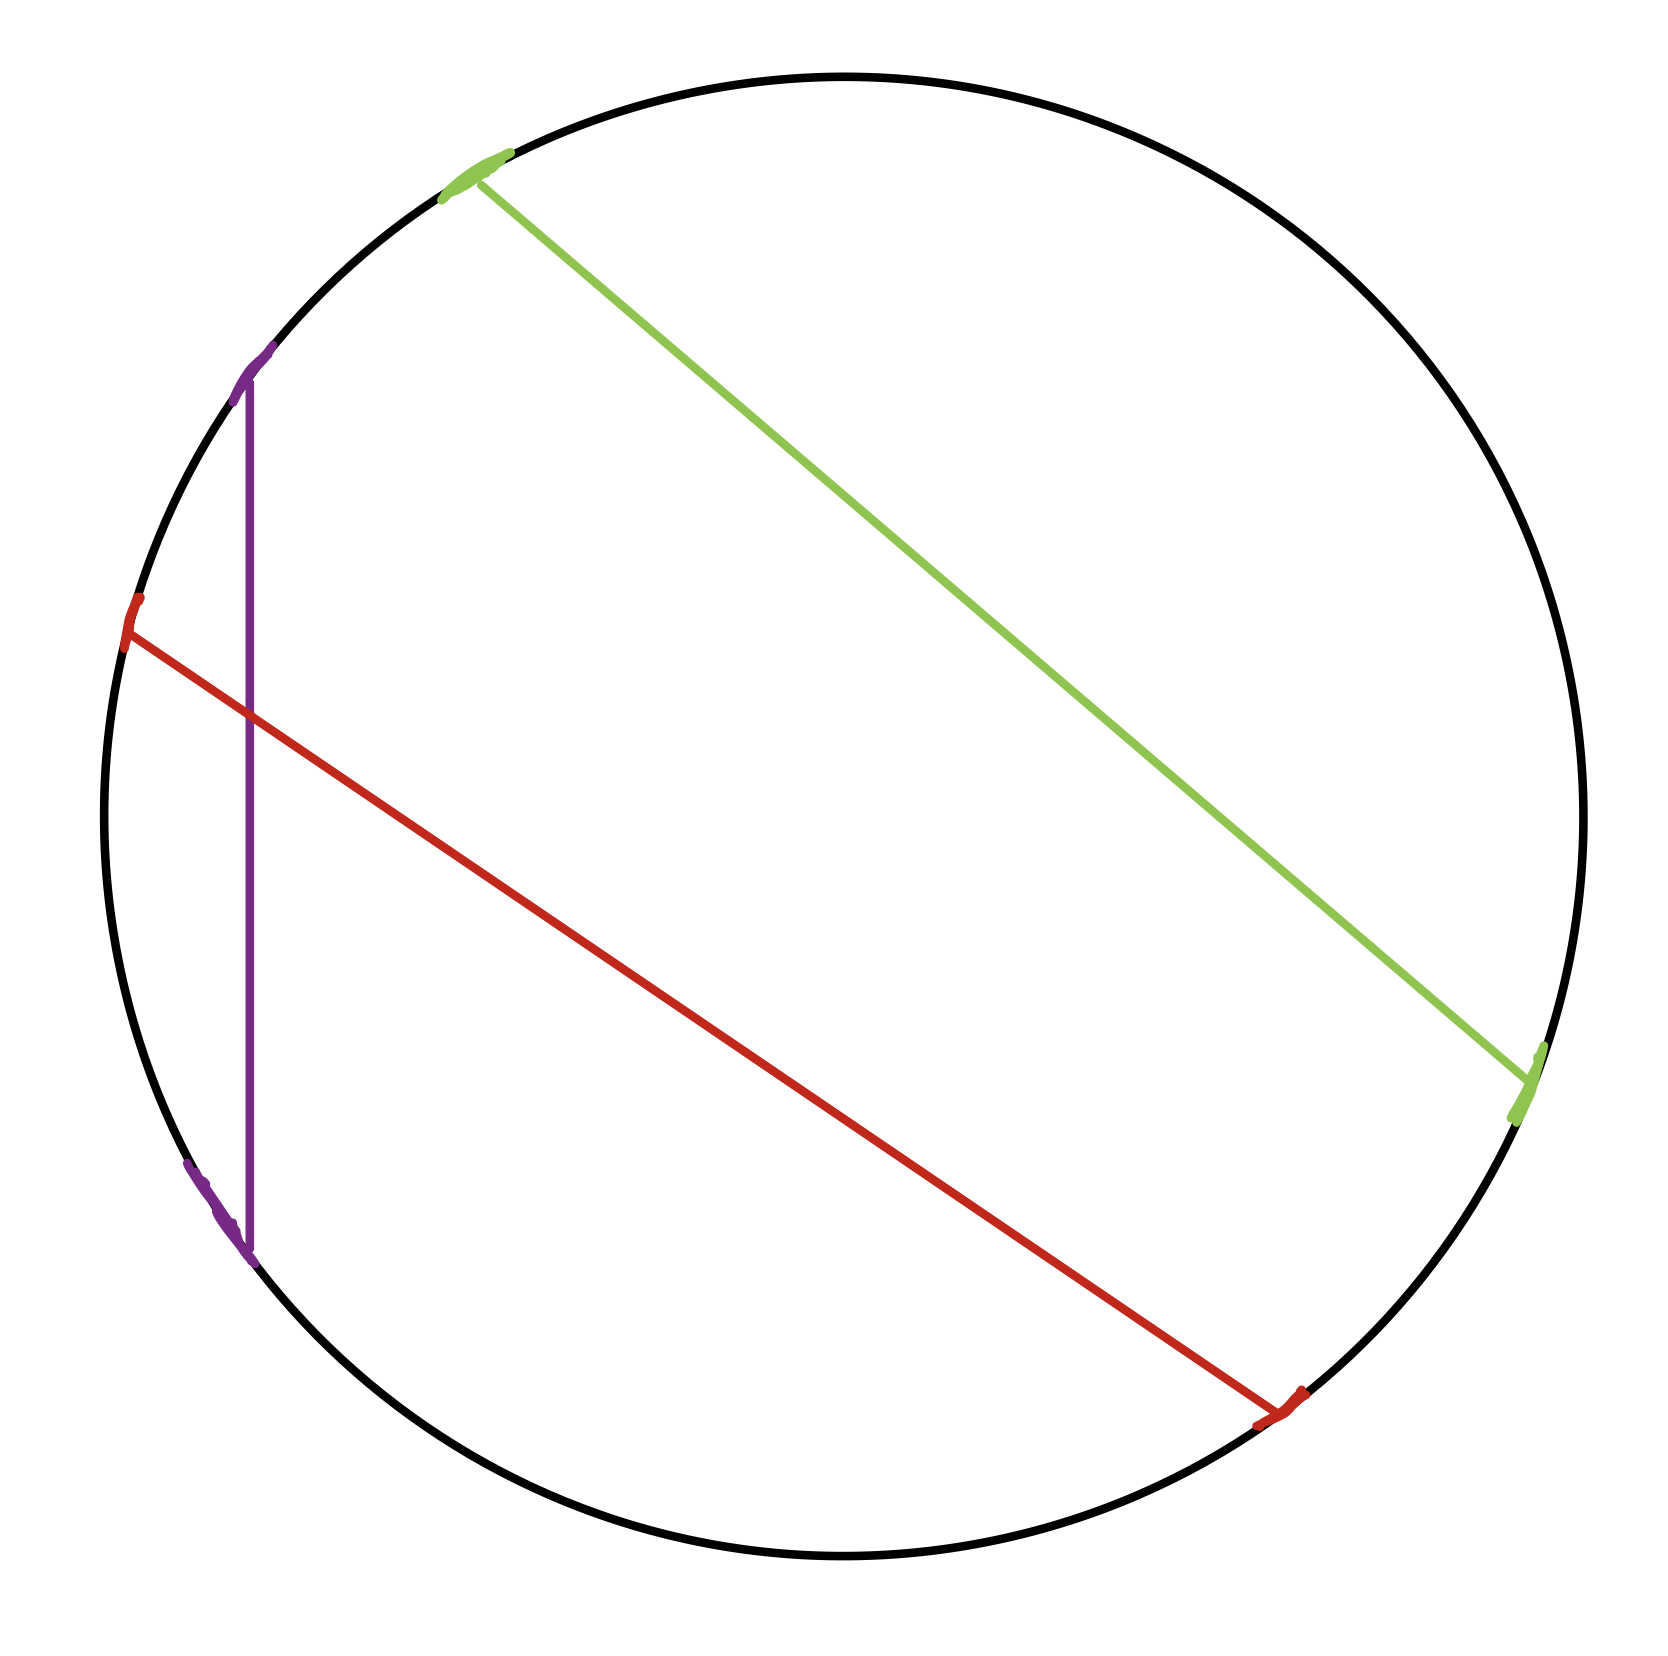
\includegraphics[width=8cm]{lehm.png}% Joonise suurus, joonise fail
    \caption{Lilla ja punase trajektooriga lehmad kohtuvad, rohelisega mitte}% Allkiri
    \allikas{Autori koostatud joonis GoodNotes abil}% Allikas
    \label{EMaxx}% Selle järgi viidatakse, pärast käsku \caption
\end{kk}
\end{solution}
\begin{cclol}
#include <bits/stdc++.h>

#include <ext/pb_ds/assoc_container.hpp>

#define pii pair < int, int >

 using namespace std;
using namespace __gnu_pbds;

typedef tree < int, null_type, less < int > , 
rb_tree_tag, tree_order_statistics_node_update > t;

int n;
bool aa[60000];
int z[60000];
int resp;

int main() {
  ios::sync_with_stdio(0);
  cin.tie(NULL);
  cin >> n;

  int c = 0;
  for (int i = 1; i < 2 * n; i++) {
    int a;
    cin >> a;

    if (aa[a]) {
      t.erase(z[a]);
      resp += t.sz() - t.order_of_key(z[a]);
      continue;
    }
    z[a] = ++c;
    t.insert(z[a]);
    aa[a] = 1;
  }

  cout << resp << endl;

  return 0;
}
\end{cclol}
\begin{kk}[H]% [] sisse märgitakse paigutus H
    \caption{Implementatsioon lahendusest ülesandele Circle Cross}% Allkiri
    \allikas{Autori implementatsioon}% Allikas
    \label{EMaxx}% Selle järgi viidatakse, pärast käsku \caption
    \end{kk}



\paragraph{Balanced Photo, USACO Gold 2017 jaanuar, ***}
\begin{extra}
Ülesannet saab esitada \href{http://www.usaco.org/index.php?page=viewproblem2&cpid=693}{USACO ametlikul veebilehel}.
\end{extra}
\begin{Text}
Põllumees Joonas rivistab oma $N$$(1\le N\le 10^5)$ lehma, et teha nendest pilti. Rivis asukohaga $i$ lehma pikkus on $h_i$, ning kõikide lehmade pikkused on erinevad.

Nagu kõikide tema lehmapiltidega, tahab Joonas, et see tuleks võimalikult ilus. Ta otsustab, et lehm $i$ näeb välja tasakaalustamata kui $L_i$ ja $R_i$ erinevad üksteisest rohkem kui kaks korda, kusjuures $L_i$ ja $R_i$ tähistavad vastavalt mitu lehma on pikemad kui $i$  lehmast vasakul ja lehmast paremal. See tähendab, et $i$ on tasakaalustamata kui $max(L_i,R_i)$ on rohkem kui kaks korda suurem kui $min(L_i, R_i)$.  Põllumees Joonas loodab, et halvimal juhul ainult mõned tema lehmadest on tasakaalustamata.

Palun aita Põllumees Joonasel leida tasakaalustamata lehmade arv.

\parencite{25}
\end{Text}
\begin{Input}
Esimesel real on $N$. Järgmisel $N$ real on $h_1,...,h_N$, millest igaüks on mittenegatiivne arv väärtusega kuni $10^9$.
\end{Input}
\begin{Output}
Väljasta tasakaalustamata lehmade arv.
\end{Output}

\textbf{Näidissisend}

\begin{verbatim}
7
34
6
23
0
5
99
2
\end{verbatim}

\textbf{Näidisväljund}

\begin{verbatim}
3
\end{verbatim}

\begin{extra}
Selles näites on tasakaalustamata lehmade pikkused 34, 5 ja 2.
\end{extra}

\begin{solution}
Me tahame leida iga lehma kohta kiiresti mitu temast pikemat lehma on temast vasakul ja paremal.

Et saavutada seda, liigume lineaarselt vasakult paremale, kasutades samaaegselt kahte indekseeritud hulka: mõlema poole jaoks üks.

Lahenduse ajakeerukuseks saame $O(N\log N)$.
\end{solution}

\begin{extra}
Meile ei sobi  std::set, sest see ei toeta indekseerimist. Lisaks, sest BBST(tasakaalustatud kahendpuu)/indekseeritud hulk ei toeta\textit{ random access}'it, on operatsioonid nagu std::distance lineaarse ajakeerukusega.
\end{extra}

\begin{cclol}
#include <bits/stdc++.h>

using namespace std;

#define ll long long
#define cint
const int

#pragma GCC optimize("O3,unroll-loops")
#pragma GCC target("avx2,bmi,bmi2,popcnt,lzcnt")

cint MA = 1e5 + 3;

#include <ext/pb_ds/assoc_container.hpp>

using namespace __gnu_pbds;
typedef tree < ll, null_type, less < ll > , rb_tree_tag, 
tree_order_statistics_node_update > inset;

int main(int argc, char ** argv) {
  ios_base::sync_with_stdio(false);
  cin.tie(NULL);
  ll n;
  cin >> n;
  array < ll, MA > arr;
  inset f;
  inset s;
  for (ll i = 0; i < n; i++) cin >> arr[i];
  array < ll, MA > smol;
  array < ll, MA > big;
  for (ll i = 0; i < n; i++) {
    smol[i] = max(0, abs((int)(i - f.order_of_key(arr[i]))));
    f.insert(arr[i]);
  }
  for (ll i = n - 1; i >= 0; i--) {
    big[i] = max(0, abs((int)(s.order_of_key(arr[i]) - (n - 1 - i))));
    s.insert(arr[i]);
  }
  ll ans = 0;
  for (ll i = 0; i < n; i++) {
  if(abs(smol[i]-big[i])>smol[i] || abs(smol[i]-big[i])>big[i]) ans++;
  }
  cout << ans;
  return 0;
}
    \end{cclol}
    \begin{kk}[H]
    \caption{USACO Gold, Balanced Photo}% Allkiri
    \allikas{Autori implementatsioon}% Allikas
    \end{kk}


\paragraph{Haircut, USACO Gold lahtine võistlus 2020, ***}
\begin{extra}
Ülesannet saab esitada \href{http://www.usaco.org/index.php?page=viewproblem2&cpid=1041}{USACO ametlikul veebilehel}.
\end{extra}
\begin{Text}
Tüdinenud oma praegusest soengust otsustab Põllumees Joonas saada uue soengu.  Tal on $N$ ($1\le N\le 10^5$) juuksekarva, ja juuksekarv $i$  on algselt pikkusega $A_i$ mikromeetrit  ($0\le A_i\le N$). Selgelt, tahab, et ta soeng oleks monotoonselt kasvav, ehk ta defineerib oma uue soengu "eepilisuse" inversioonide arvuna kujul: paarid ($i,j$), kus $i<j$ ja $A_i>A_j$.

Iga $j=0,1,…,N−1$ kohta,  Joonas tahab teada oma soengu eepilisust, juhul kui kõik juuksekarvad, mis on pikemad kui $j$ lõigatakse pikkuseni täpselt $j$.

\parencite{26}
\end{Text}

\begin{Input}
\[N\]
\[A_1, A_2, ..., A_N\]

\end{Input}

\begin{Output}
Iga  $j=0,1,…,N−1$ kohta, väljasta Joonase soengu eepilisus.
\end{Output}



\textbf{Näidissisend}

\begin{verbatim}
5
5 2 3 3 0
\end{verbatim}

\textbf{Näidisväljund}

\begin{verbatim}
0
4
4
5
7
\end{verbatim}


\begin{solution}
Iga $0≤j<N$ kohta me peame arvutama paaride arvu $(x,y)$ kus $x<y$,  $A[x]>A[y]$ ja $A[y]<j$. 
Piisab sellest, et arvutada $x<y$ hulk kus $A[x]>A[y]$ iga $y$ kohta; nimetame seda $n[y]$. 
Siis oleks vastus: $ans[j]=∑_{A[y]<j}n[y]$, saame kasutada prefiksi summa võtet.

$n[y]$ väärtuse iga $y$ kohta saab leida järgnevalt:
\begin{enumerate}
    \item  Tee $h=N$.
    \item   Salvesta indeksite hulka, mis on algselt tühi.
    \item  Iga $y$ kohta kus $A[y]=h$, märgi ära $y$ väärtuseks arv hulgas mille väärtus on väiksem kui $y$.
    \item  Iga $y$ kohta kus  $A[y]=h$, lisa hulka $y$.
    \item  Kui $h=0$, lõpeta programmi töö. Vastasel juhul, vähenda $h$ väärtust ühe võrra ja korda protsessi alates sammust 2.
\end{enumerate}

\begin{kk}[H]% [] sisse märgitakse paigutus H
    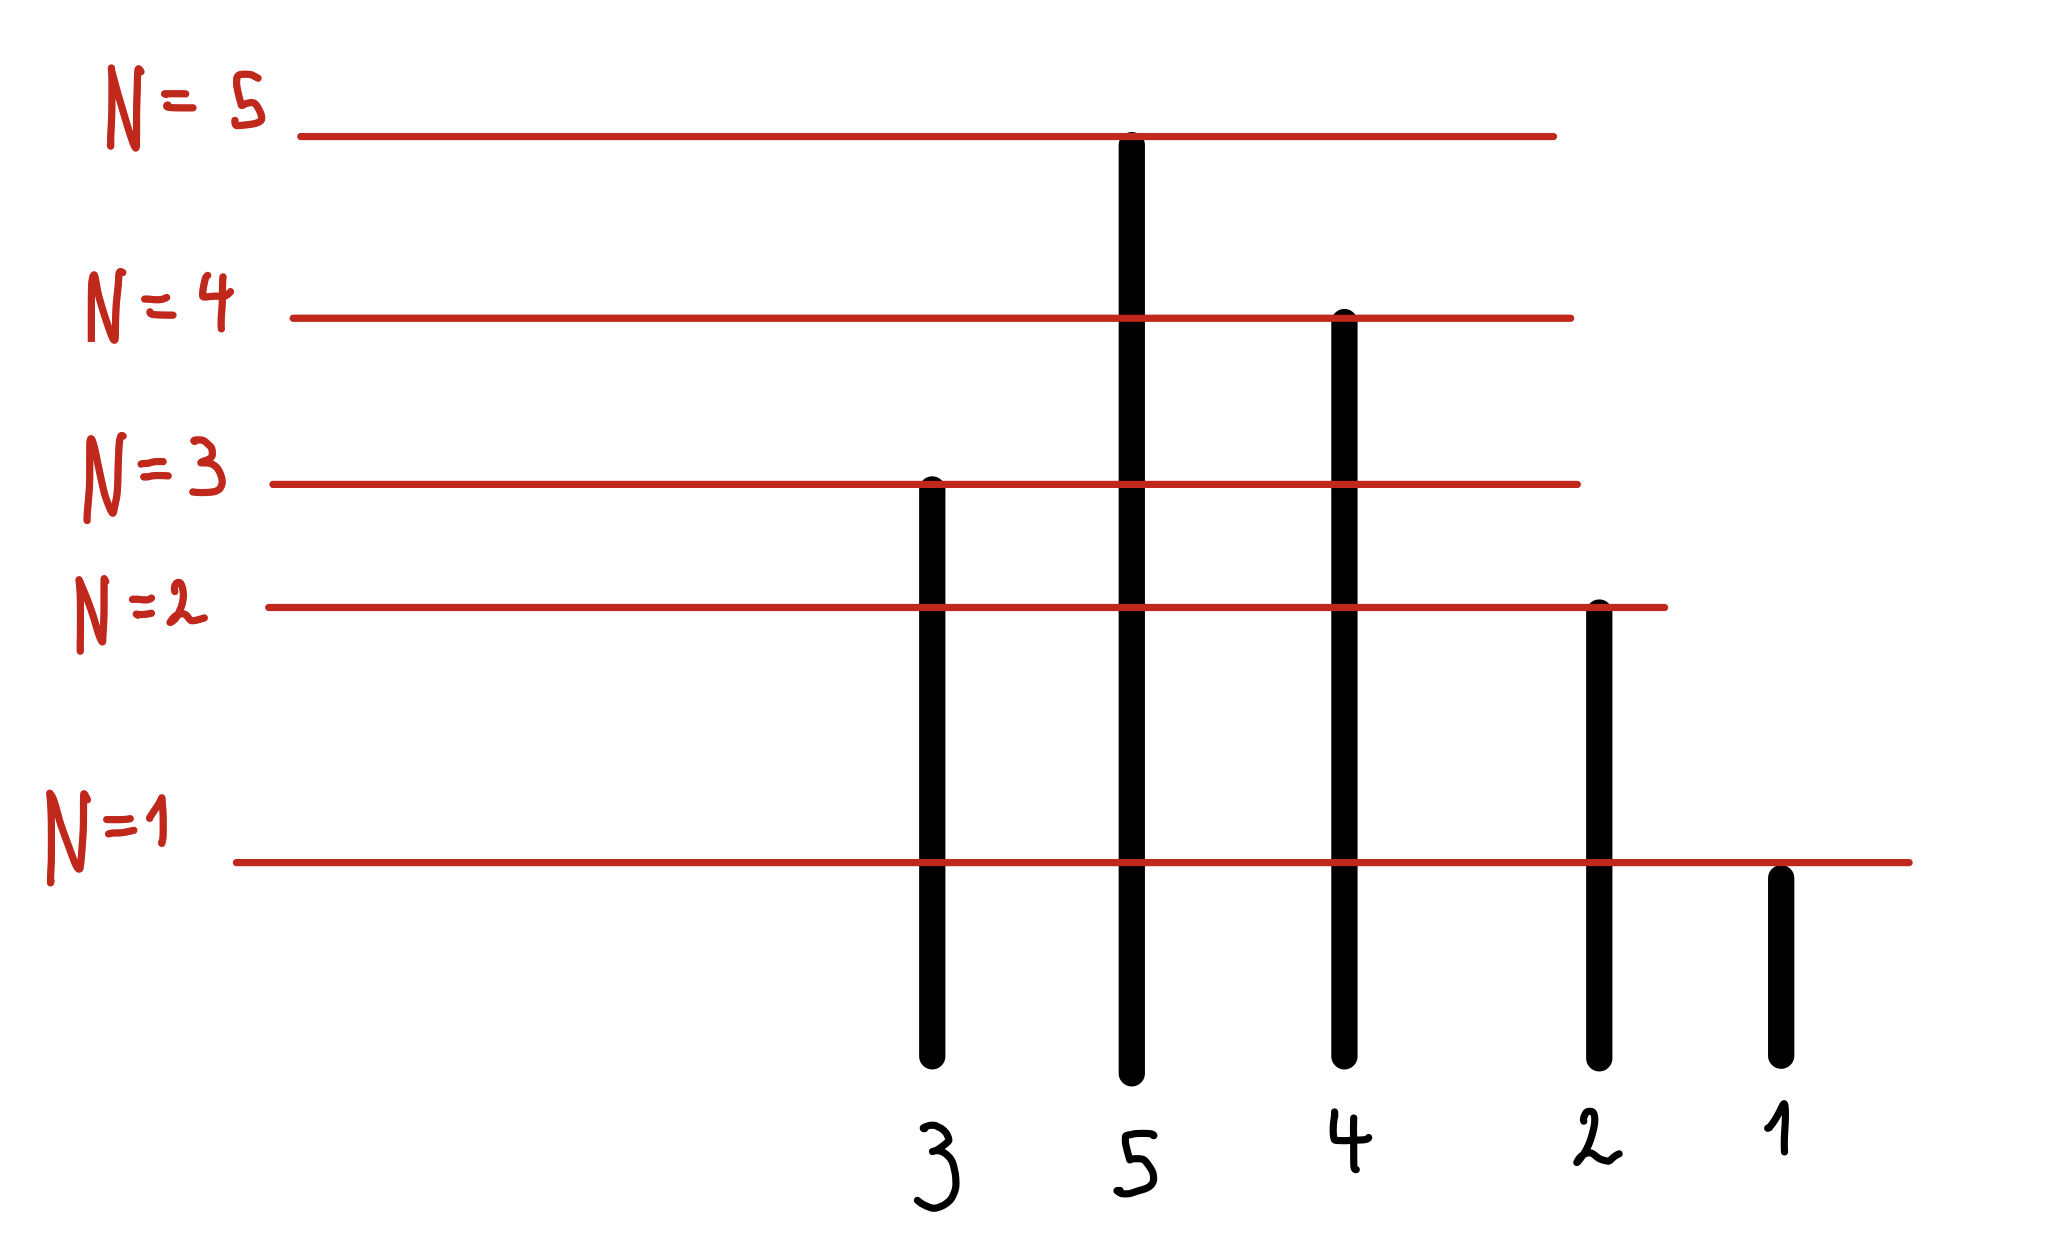
\includegraphics[width=8cm]{jooned.png}% Joonise suurus, joonise fail
    \caption{Juuksekarvade lõikamine}% Allkiri
    \allikas{Autori koostatud joonis GoodNotes abil}% Allikas
    \label{EMaxx}% Selle järgi viidatakse, pärast käsku \caption
\end{kk}

Selle jaoks sobib ideaalselt indekseeritud hulk.
\end{solution}

\begin{cclol}
#include "bits/stdc++.h"

using namespace std;

#include <ext/pb_ds/assoc_container.hpp>

using namespace __gnu_pbds;
typedef tree < int, null_type, less < int > , 
rb_tree_tag, tree_order_statistics_node_update > inset;

const int MA = 1e5 + 5;

int n;
long long Inv[MA];
vector < int > todo[MA];

int main() {
  ios_base::sync_with_stdio(false);
  cin.tie(NULL);
  int n;
  cin >> n;
  vector < int > A(n);
  for (int & t: A) cin >> t;
  for (int i = 0; i < n; ++i) todo[A[i]].push_back(i);
  inset T;
  for (int i = n; i >= 0; --i) {
    for (int t: todo[i]) Inv[i + 1] += T.order_of_key(t);
    for (int t: todo[i]) T.insert(t);
  }
  for (int i = 1; i < n; ++i) Inv[i] += Inv[i - 1];
  for (int i = 0; i < n; ++i) cout << Inv[i] << endl;
}
\end{cclol}
\begin{kk}[H]
    \caption{USACO Gold, Haircut}% Allkiri
    \allikas{Autori implementatsioon}% Allikas
    \end{kk}
\paragraph{Sleepy Cow Sorting, USACO Gold 2019 jaanuar, ****}
\begin{extra}
Ülesannet saab esitada \href{http://www.usaco.org/index.php?page=viewproblem2&cpid=898}{USACO ametlikul veebilehel}.
\end{extra}
\begin{Text}
Põllumees Joonas tahab järjestada oma $N$ lehma($1\le N\le 10^5$), nummerdatud $1…N$, enne seda kui lehmad liiguvad edasi hommikust sööma.
Praegusel hetkel, seisavad reas järjekorras $p_1,p_2,p_3,…,p_N$, ning Põllumees Joonas seisab lehma $p_1$ ees. Ta tahab järjestada lehmad niimoodi, et nad oleks järjekorras $1,2,3,…,N$, kus lehm 1 seisab Põllumees Joonase kõrval.

Täna on lehmad natuke väsinud, ehk ainus lehm, kes igal ajahetkel  kuulab Joonase juhiseid tähelepanelikult on lehm kes seisab otse Põllumees Joonase ees. Ühel ajahetkel, saab ta käskida sellel lehmal liikude $k$ samme reas edasi, iga $k$ kohta $1$ ja $N−1$ vahel(kaasa arvatud). $k$ lehma kellest see lehm möödub teevad talle eeskujulikult ruumi, et ta saaks jõuda reas nende taha.

Näiteks, ütleme, et $N=4$ ja lehmad on algselt reastatud järgnevalt:

Joonas: 4, 3, 2, 1 

Ainus lehm kes kuulab tähelepanelikult Joonast on lehm $4$. 
Kui ta annab talle juhised liikuda $2$ sammu read edasi, siis näeks rida välja selline:

Joonas: 3, 2, 4, 1 

Nüüd kuulab Joonast ainult lehm $3$, ehk praegusel ajahetkel ta saab anda lehmale $3$ juhise, ja nii edasi kuni kõik lehmad on korrektselt järjestatud.

Põllumees Joonas peab seesugust järjestamist ülimalt tähtsaks, et ta saaks minna tagasi oma majakesse ise hommikusööki nautima. 
Aita tal leida selline juhiste kombinatsioon, mis reastab lehmad võimalikult lühikese ajaga.

\parencite{27}
\end{Text}

\begin{Input}
Esimesel sisendireal on  $N$. 
Teisel real on $N$ tühikuga eraldatud täisarvu: $p_1,p_2,p_3,…,p_N$, tähistades esialgset lehmade järjestatust.
\end{Input}

\begin{Output}
Esimesel real peaks olema üksainus täisarv $K$, mis tähistab minimaalset aega, mida on vaja lehmade korrektselt järjestamiseks.
Teine rida peaks sisaldama $K$ tühikuga eraldatud täisarvu, $c_1,c_2,…,c_K$, igaüks vahemikus $1…N−1$. Lisaks, juhul kui $i$-ndal ajahetkel annab Põllumees Joonas juhised lehmale otse tema ees liikuda $c_i$ sammu read ettepoole, siis pärast $K$ ajahetke peaksid lehmad olema õigesti järjestatud.

Kui leidub mitu võimalust minimaalse ajaga korrektselt lehmad järjestada, väljasta ükskõik milline nendest.
\end{Output}



\textbf{Näidissisend}

\begin{verbatim}
4
1 2 4 3
\end{verbatim}

\textbf{Näidisväljund}

\begin{verbatim}
3
2 2 3
\end{verbatim}


\begin{solution}
Kui vastus on $k$, mida see tähendab? Kui vastus on $k$, siis üksgi lõplik $n-k$ lehmadest ei muuda oma järjekorda üksteise suhtes, ehk nad peavad olema juba korrektselt järjestatud.

Sellega saame $k$-le alampiiri. Selgub, et see annab ka vastuse, põhjusel, et saame sisestada ülejäänud lehmad oma õigetele positsioonidele viimase $k$ jooksul. 

Näiteks: $(3,4,5,2,(1,6))→(4,5,2,(1,3,6))→(5,2,(1,3,4,6))→(2,(1,3,4,5,6))→(1,2,3,4,5,6)$

Nüüd on vaja leida juhiste järjestus pikkusega $n-k$.  Esimene juhis oleks sorteeritud lehmade arv miinus üks ja sorteeritud lehmade arv korrektselt järjestatud suffiksis(millel on indeksid väiksemad kui praegu vaadeldaval lehmal) summa.  Varem toodud näites peaks esimene lehm liikuma $3+1$ sammu edasi.

Pärast eelmist juhist on esimene lehm järjestatud suffiksi osa, teeme rekursiivselt sama uuesti. Kuid selletaolise naiivse algoritmi ajakeerukuseks oleks $O(N^2)$.

Seda saab kiirendada andmestruktuuriga mis hoiab hulka $S\subseteq \{1,...,n\}$ ja võimaldab järgmisi operatsioone effektiivselt: 
\begin{enumerate}
    \item $x\in \{1,...,n\}$ kohta, sisesta $x$ $S$-i.
    \item $y\in \{1,...,n\}$, leia elementide arv $S$-is, mille väärtus on väiksem kui $y$.
\end{enumerate}

Selliseid andmestruktuure on mitmeid, kuid autori arvates on nendest lihsaim indekseeritud hulk.
\end{solution}
\begin{cclol}
#include <bits/stdc++.h>

using namespace std;

#include <ext/pb_ds/assoc_container.hpp>

using namespace __gnu_pbds;

typedef tree < int, null_type, less < int > , 
rb_tree_tag, tree_order_statistics_node_update > inset;

int main() {
  ios_base::sync_with_stdio(false);
  cin.tie(NULL);

  int N;
  cin >> N;
  vector < int > a(N);
  inset oset;
  for (int i = 0; i < N; i++) cin >> a[i];
  int ptr = N - 1;
  for (int i = N - 1; i >= 0; i--) {
    if (i == N - 1 || a[i] < a[i + 1]) {
      ptr--;
      oset.insert(a[i]);
    } else break;
  }
  cout << ptr + 1 << endl;
  for (int i = 0; i <= ptr; i++) {
    oset.insert(a[i]);
    if (i) cout << " ";
    cout << (oset.order_of_key(a[i]) + (ptr - i));
  }
  cout << endl;

  return 0;
}
\end{cclol}
\begin{kk}[H]
    \caption{USACO Gold, Sleepy Cow Sorting lahendus}% Allkiri
    \allikas{Autori implementatsioon}% Allikas
    \end{kk}
\section{Nõuandeid võistlusel hea tulemuse saavutamiseks}
Autor soovitab kasutada võistlusel lihtsalt seda võtet mis on kõige jõukohasem implementeerida, isegi olukorras kus selline lahendus ei ole piisavalt kiire, sest olümpiaadil saab siis tõenäoliselt mõned punktid alamülesande eest siiski.

Kui lihtsam lahendus on algselt napilt liiga aeglane, siis on ka võimalus, mõõta aega(vt Lisa 5), leides nn pudelikael, ning proovides optimeerida lahendust(vt Lisa 6, 7).

Olukorras, kus lahendus on piisavalt kiire, kuid töötab ainult mõningal korral, kuid saamata aru teksti lugedes milles on viga(tõenäoliselt valed indeksid), saab ka kasutada, testide genereerimist. Eriti hästi töötab mainitud võte siis kui kirjutada sama funktsionaalsusega koodist kaks versiooni, üks mis on vigane, kuid oleks teoorias võimeline andma ülesandes punkte, ja teine mis on liiga aeglane, kuid annab kindlasti õige vastuse. Seejärel saab genereeritud testid sisestada mõlemale programmile ja vaadata kus erineb vastus, niimoodi ongi kindel problemaatiline koht leitud.
Mainitud viis vigade leidmiseks on ajamahukas, kuid alati üsnagi tulemuslik, ehk see on parem ikkagi kui lihtsalt ekraani vahtimine.

Et võistlusel saada hea tulemus, on kõige tähtsam ikkagi harjutada lahendades varasemaid ülesandeid selleks on, juhul kui osata inglise keelt, internetis väga palju võimalusi.
\section{Autori koostatud ülesanded ja sellest tulenevad järeldused}

Autor koostas kõik ülesanded Polygon(Codeforces) süsteemi abil, ning on soovi korral esitatavad samal platvormil.

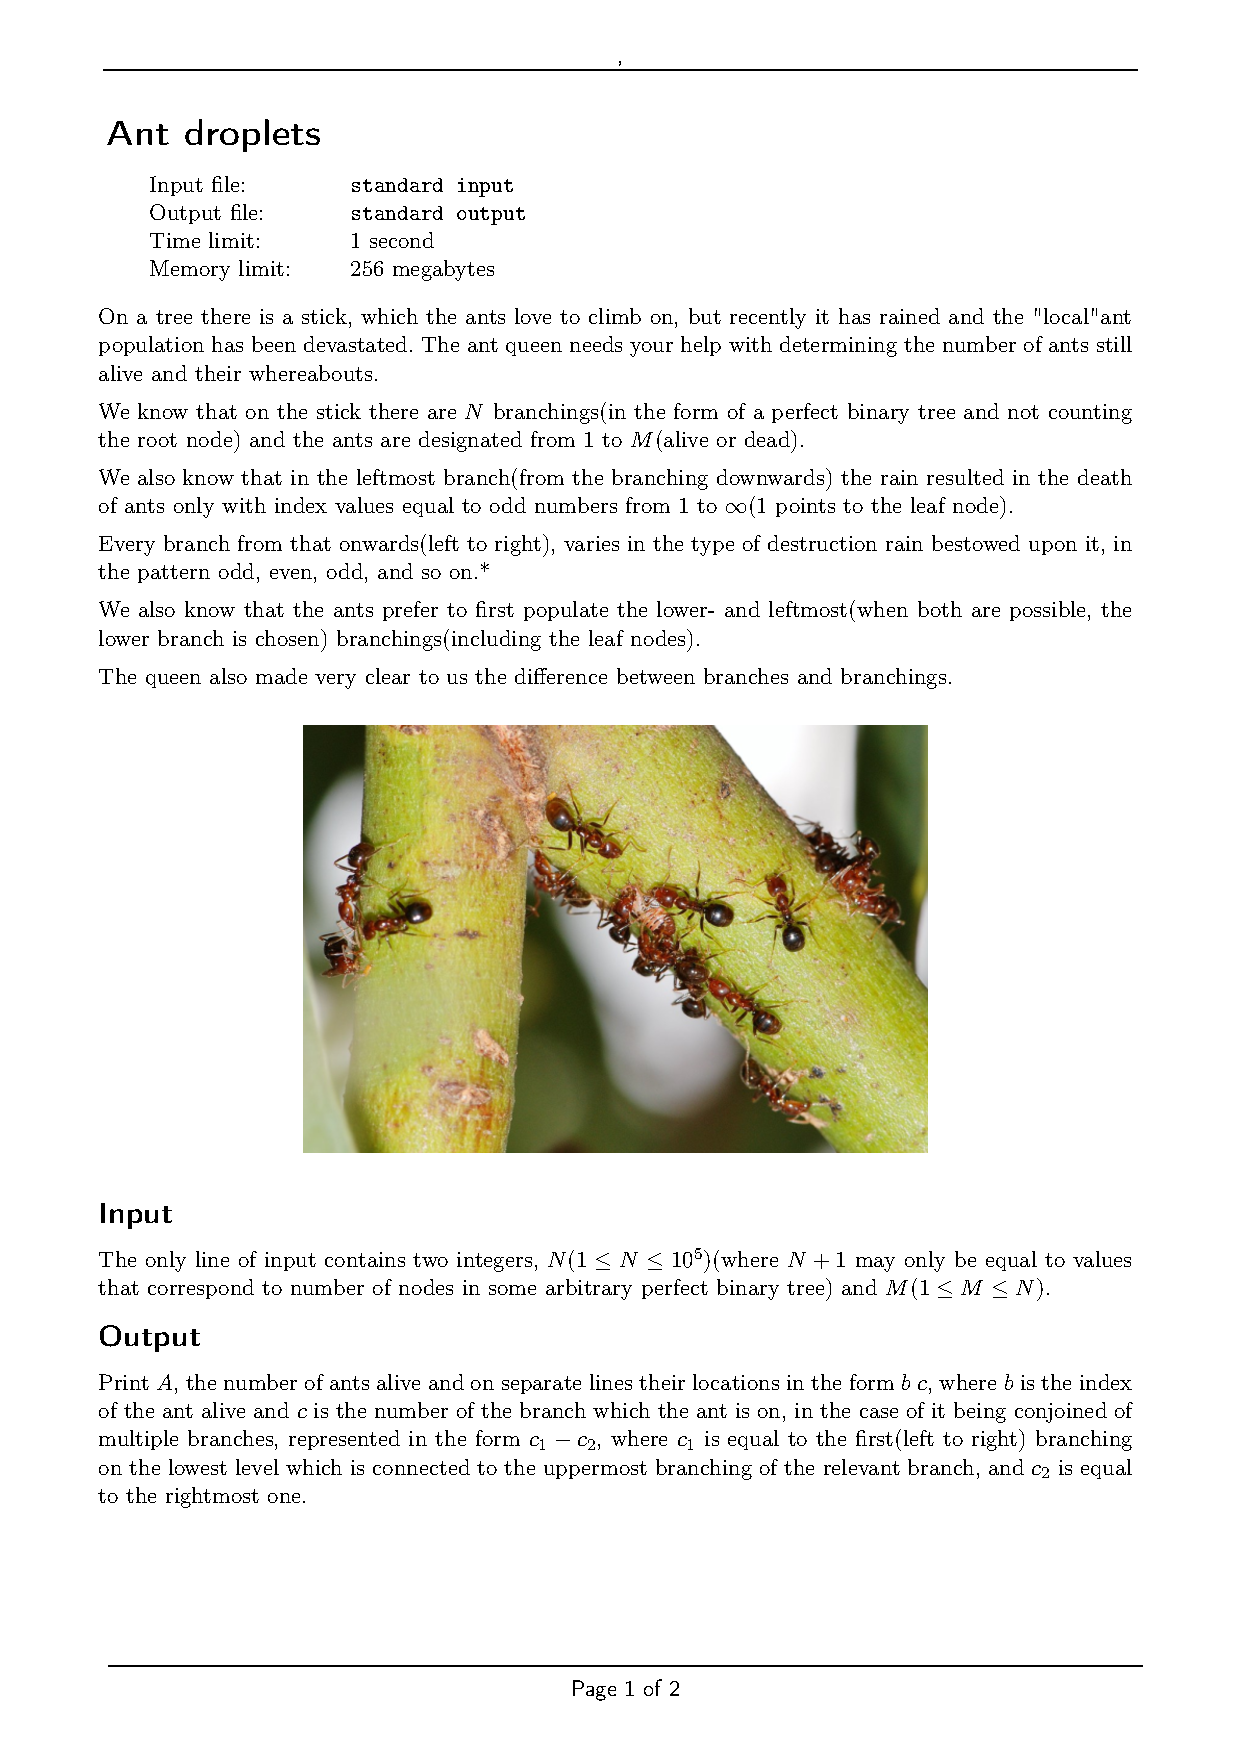
\includepdf[pages=-]{antdroplets.pdf}


Implementatsioon on väga lihtne kuigi valemi tuletamiseni on jõuda oluliselt raskem.
    \begin{cclol}
 #include <bits/stdc++.h>

 using namespace std;
 int main(int argc, char ** argv) {
   int n, m;
   cin >> n >> m;
   int x = min(n, m) / 2;
   cout << x << endl;
   for (int i = 1; i <= x; ++i) {
     cout << i * 2 << " " << i * 2 << endl;
   }
   return 0;
 }
    \end{cclol}
    \begin{kk}[H]% [] sisse märgitakse paigutus H
    \caption{Autori implementatsioon}% Allkiri
    \label{mkm}% Selle järgi viidatakse, pärast käsku \caption
    \end{kk}

    Implementatsiooni lihtsus tuleneb sellest et käsitleme perfektset kahendpuud, ning seda liiki puu järgib kindlaid mustreid, nagu nt tippude arv igal tasemel ülemiselt alumisele on võrdne kahe astmega ja moodustab geomeetrilise jada $2^0...2^T$, kus $T$ on tasemete arv. 
    Sellest on lihtne täheldada, et lehtede arv $lArv = \frac{N+1}{2}$, kus $N$ on tippude arv koos juurtipuga.

    Edasi minnes saab täheldada, et ainsad tipud kus peame üldse teada saama kas sipelgas jääb ellu või mitte on puu lehed, ning need ka on matemaatiliselt leitavad s.t et teame et iga paaris indeksiga puu lehel oleva sipelgas jäi ellu. Sellepärast et lehtede arv kahendpuus on alati paarisarv, saame järeldada et alumisel tasemel jäi sipelgaid ellu $M/2$, kus $M$ on algne sipelgate arv.

    Aga mida teha siis kui sipelgate arv on väiksem kui puu lehtede arv, siis on vastus ikkagi lihtsasti leitav, sellepärast et iga paaritu indeksiga sipelgas on surnud ning ei tohi neid arvestada, peame lihtsalt ümardama vastuse allapoole, mida nt C++ teeb automaatselt(kui proovida suruda komaarv, integer andmetüüpi).

    Selle jaoks, et teada kumbat olukorda, kasutame standardset $min()$ funktsiooni.

    Sipelgate indeksid saavad olla võrdsed ainult paarisarvudega, ning puu oksa(branch) indeks olla ainult võrdne sellel asetseva sipelga indeksiga(sest jälgime ainult puu lehti), seda teades väljastamegi lihtsalt kõik paarisarvud $\le x$ kahekordselt.


    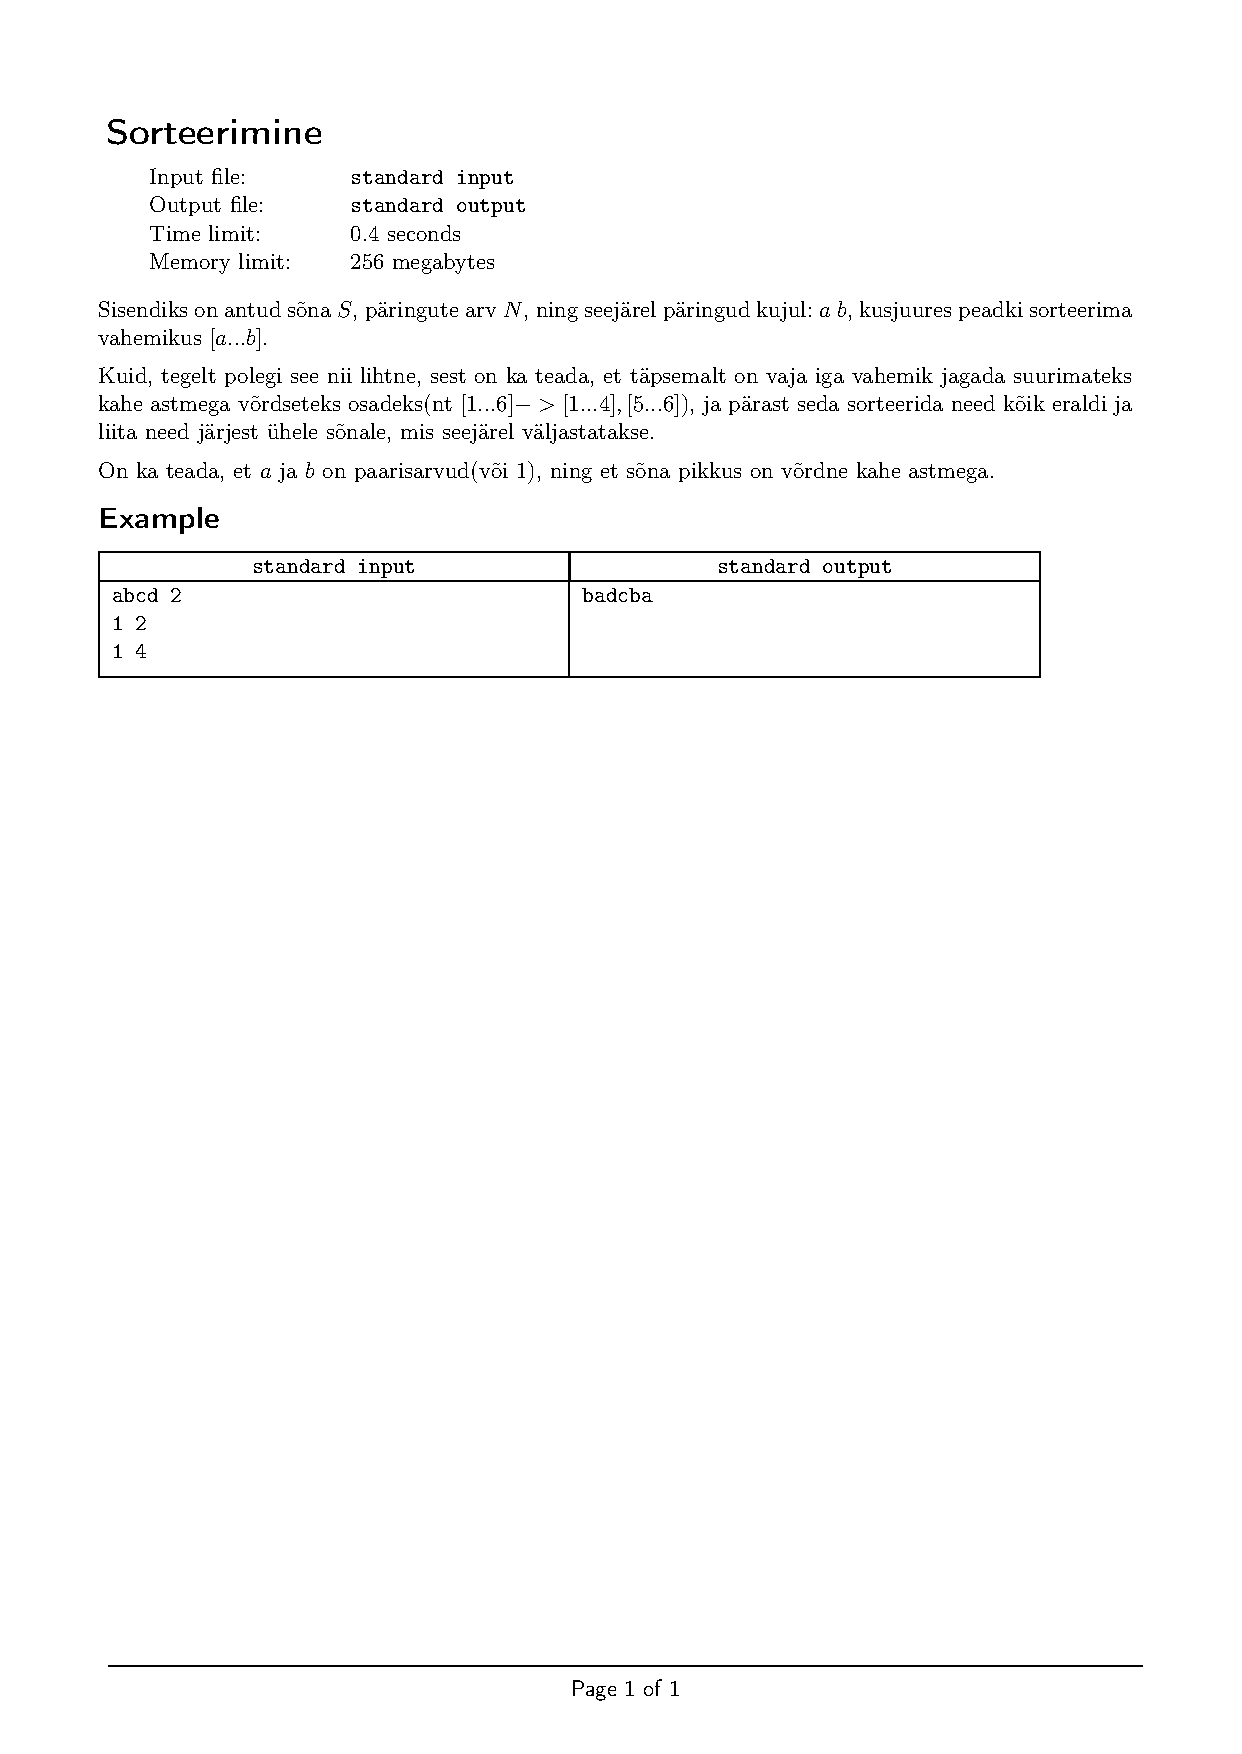
\includepdf[pages=-]{failin.pdf}

Esimene autori poolt loodud lõikude puuga lahendamiseks mõeldud ülesanne, osutuski lahendatavaks lihtsa valemiga ja nelja rea koodiga, kuid tegu oli siiski üsnagi huvitava lihtsamat sorti arvuteooria ülesandega, mis sobiks täitsa nt Eesti Informaatikaolümpiaadi lahtise võistluse esimeseks või teiseks ülesandeks.
Raskeks osutus kuigi arusaadava ja selge(ka kompaktse) teksti koostamine, millest saaksid kõik ühtemoodi aru.  

Õppides esimese vigadest, on teine autori poolt loodud ülesanne oluliselt lühema ja ka seepärast arusaadavama tekstiga. 
Ülesannet on ka oluliselt raskem lahendada ilma lõikude puuga.
Teise ülesande loomisele kulus oluliselt kauem aega, kui esimese loomisele, sest autor proovis tagada, et ülesanne on kiiresti lahendatav ainult lõikude puuga. 

Lahendus teisele ülesandele on jäetud lugejale koduseks tööks.

Autori järelduseks on see, et ülesannete loomine pole sugugi nii lihtne kui ta algselt arvas.

Lugedes Codeforces blogi seotud teemal, järeldab veel autor, et lihtsam on koostada ülesandeid kui sa toetud varasematele ülesannetele, tehes neid kas raskemaks või lihtsamaks omaduste/nõuete muutmisega \parencite{problemsetting}.

\addchap{Kokkuvõte}

Uurimistöös käsitleti lõikude puu andmestruktuuri ja selle kasutusvõimalusi võistlusprogrammeerimises. Praktilises osas koostas autor kaks lõikude puuga seotud ülesannet, andis nõuandeid võistlusprogrammeerimises selliste ülesannete lahendamiseks, tõi välja andmestruktuuri plusse ja miinuseid, ning lahendas ja selgitas mitmeid erinevaid lõikude puuga lahendatavaid ülesandeid.

Praktilises osas selgus, et lõikude puu on võistlusprogrammeerimises väga kasulik andmestruktuur nii kasutusvõimaluste ja ajakeerukuse poolest, kuid tegu on algajale ikkagi suhteliselt raskesti implementeeritava andmestruktuuriga ja enamasti saab seda asendada mingi sarnase, kuid lihtsama võttega. Eriti kasulikuks avastuseks oli autori arvates indekseeritud hulga andmestruktuur, mis on GNU kompilaatoriga kaasas, ning võimaldab väga lihtsalt, kuid efektiivselt teha paljusi operatsioone.

Uurimistöö käsitles teoreetilises osas põhiliselt kõiki senini võistlusprogrammeerimises kasutatud lõikude puuga seotud võtteid, kuid uurimistööd saab laiendada, tuues välja rohkem näiteid ja neid üksikasjalikumalt täiendades.


\printbibliography


\begin{appendices}

    \chapter{Graafiteooria põhimõisted}\label{lisa1}
    \normalsize
    Graaf on teoreetiline struktuur millele omane tunnud on tipud mis on omavahel ühendatud servadega.
    
    Graafi servad võivad olla ka kaalutud, s.t et servadel on arvuline väärtus mis kujutab mööda tippu liikumise "maksumust".

    Seostatud tipupaari nimetatakse naabertippudeks. \parencite{graaf}
    
    \begin{figure}[H]% [] sisse märgitakse paigutus H
    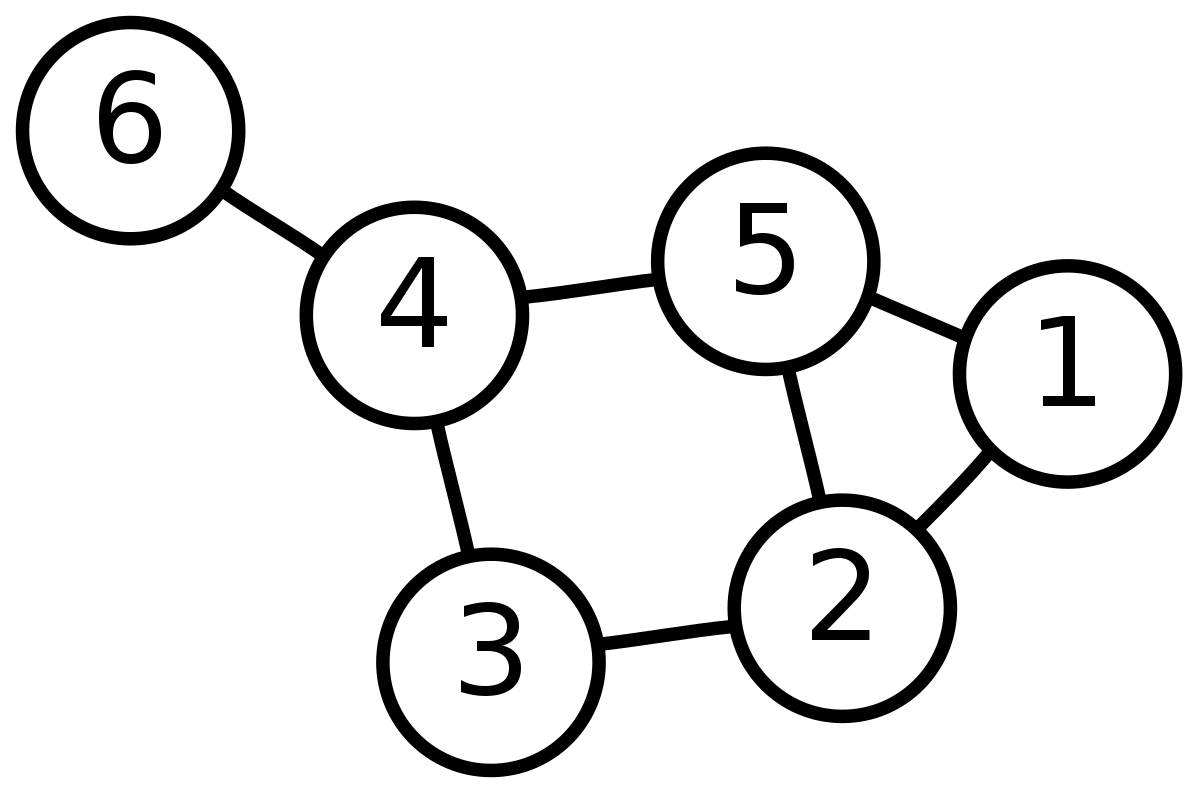
\includegraphics[width=8cm]{graaf.png}% Joonise suurus, joonise fail
    \caption{Graafi struktuur}% Graafi struktuur
    \allikas{Vikipeedia}% Allikas
    \label{graaf}% Selle järgi viidatakse, pärast käsku \caption
    \end{figure}



    \chapter{Graafitüüp nimetusega puu}\label{lisa2}
    \tiny
    \normalsize

    Puu on sidus ja tsükliteta graaf, s.t et graaf kuulub ühte sidususkomponenti, ehk liikudes mööda graafi servu on võimalik jõuda ühest tipust ükskõik millisesse teisse tippu, tsükliteta tähendab seda, et puuduvad "tsirkulaarsed" teekonnad, formaalsemalt tähendab see ka seda et servade arv on $N-1$, kus $N$ on tippude arv.

    Puu juurtipu määramine seisneb sellest et justkui riputatakse puu ühte tippu pidi seina külge, ehk puu juur on vabalt määratletud.

    Puu lapstippudeks nimetatakse juurtipuga puus, tipu naabertippe mis asuvad allpool, vanemtippud asuvad ülevalpool. \parencite{puu}
   
    \begin{figure}[H]% [] sisse märgitakse paigutus H
    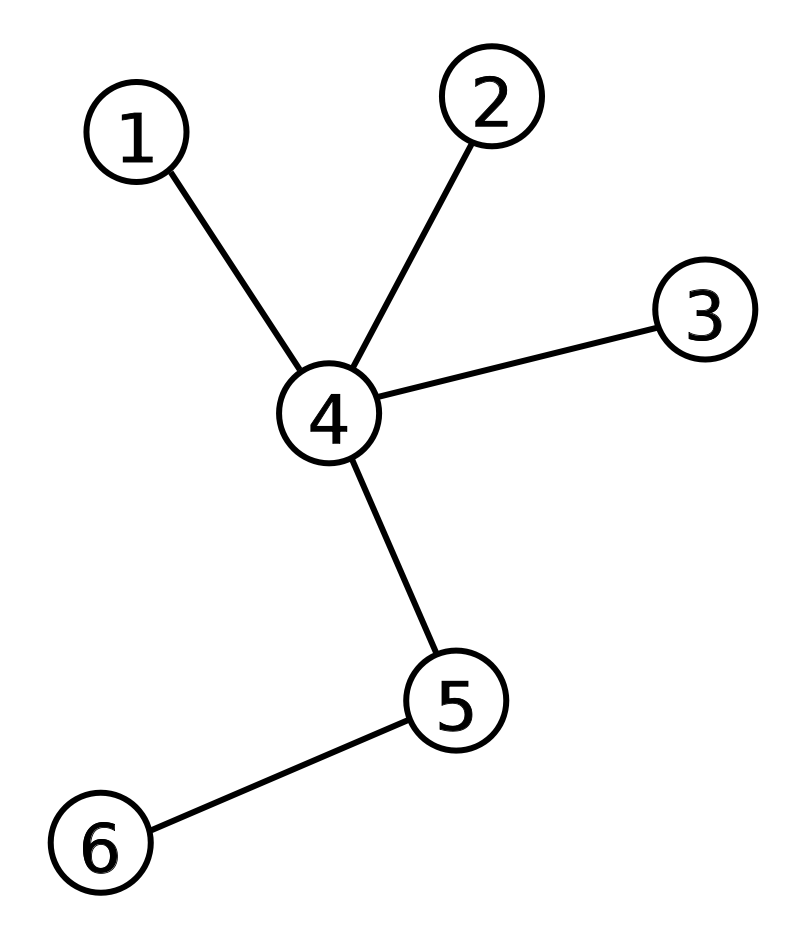
\includegraphics[width=8cm]{puu.png}% Joonise suurus, joonise fail
    \caption{Puu struktuur}% Allkiri
    \allikas{Vikipeedia}% Allikas
    \label{puu}% Selle järgi viidatakse, pärast käsku \caption
    \end{figure}

\chapter{Puu läbimise meetodid}\label{lisa3}
    \tiny
    \normalsize
    \begin{figure}[H]% [] sisse märgitakse paigutus H
    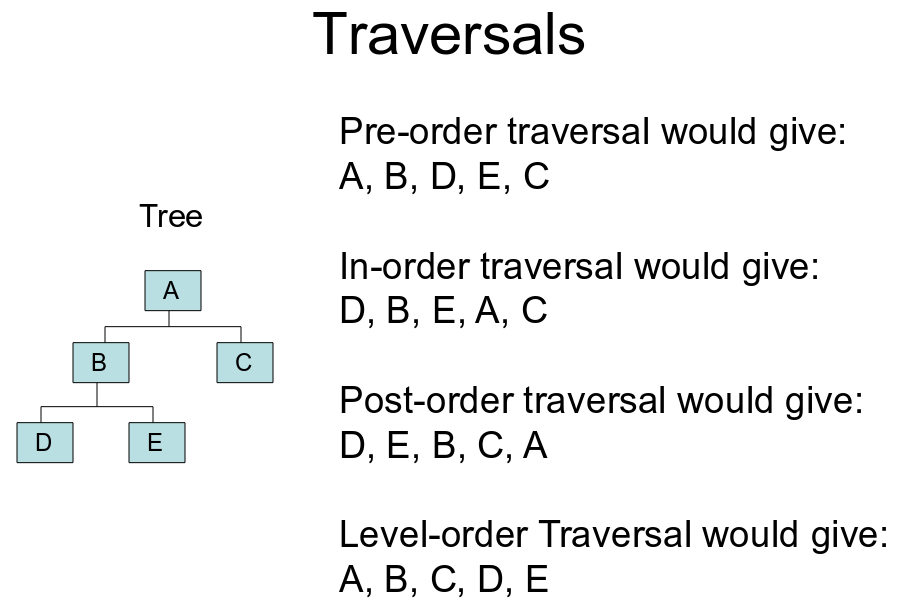
\includegraphics[width=14cm]{traversal.png}% Joonise suurus, joonise fail
    \caption{Puu läbimine}% Allkiri
    \allikas{Intermediate Computing with Data Structures CS210}% Allikas
    \label{pragmas}% Selle järgi viidatakse, pärast käsku \caption
    \end{figure}
    Joonisel on välja toodud erinevad puu läbimise meetodid ja selle põhjal ehitatav massiiv\parencite{cohen}.

\chapter{C++ fundamentaalsed andmetüübid}\label{lisa4}
    \tiny
    \normalsize
    
    \begin{table}[H]% [] sisse märgitakse paigutus H
    \caption{Andmetüübid}% Allkiri
    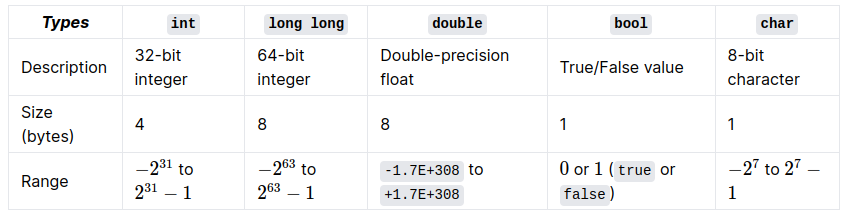
\includegraphics[width=14cm]{datatypes.png}% Joonise suurus, joonise fail
    \allikas{USACO Guide. Datatypes}% Allikas
    \label{pragmas}% Selle järgi viidatakse, pärast käsku \caption
    \end{table}

    Üldiselt võib ka lihtsalt terve programmi vältel igaks juhuks kasutada $long\ long$ andmetüüpi, erandiks on muidugi juhud, kui nt ülesandel on väiksed mälulimiidid, või on lihtsalt vaja luua, näiteks $10^5$ suurune massiiv.

    Kui kasutada suuremamahulisi andmetüüpe ainult mõnes kohas, siis on tähtis teada, et näiteks bitioperatsioonid või tehted kujul $(long long) a = (int) b$, võivad anda valeseid vastuseid.

    GCC kompileerija toetab ka $128$ bitist andmetüüpi, juhul kui arvuti riistvara võimaldab seda.
    
    Python'i kasutajatel ei ole üldjuhul vaja muretseda, sest tegu on interpreteeritava keelega, mis teeb integeride intialiseerimist oluliselt mugavamaks kiiruse arvel, ja toetab ka nn lõpmatu suurusega $bignum$ andmetüüpi\parencite{usaco2}.

 \chapter{Algoritmi kiiruse määramimine}\label{lisa5}
    \tiny
    \normalsize
    Kiirust saab lihtsati mõõta C++ teegiga $<chrono>$, teine lihtne võimalus, juhul kui algoritmi kasutav ülesanne on kättesaadav Codeforces(või Polygon) keskkonnas, on 
    kasutada Polygon Invocation süsteemi või Codeforces ülesande esitamist.

    \begin{cclol}
using namespace std::chrono_literals;

template < class DT = std::chrono::milliseconds,
  class ClockT = std::chrono::steady_clock >
  class Timer {
    using timep_t = decltype(ClockT::now());

    timep_t _start = ClockT::now();
    timep_t _end = {};

    public:
      void tick() {
        _end = timep_t {};
        _start = ClockT::now();
      }

    void tock() {
      _end = ClockT::now();
    }

   template < class duration_t = DT >
    auto duration() const {
    // Use gsl_Expects if your project supports it.
    assert(_end != timep_t {} && "Timer must toc before reading time");
    return std::chrono::duration_cast < duration_t > (_end - _start);
    }
};
    \end{cclol}
    \begin{kk}[H]
    \caption{Programmi jooksutamisaja mõõtmine millisekundites}% Allkiri
    \allikas{Nikos Athanasiou Stack Overflow vastus}% Allikas
    \end{kk}
    Vajalik on ka $Timer$'i nt nimega clock intialiseerimine, see tähendaks et saaksime kasutada järgnevat koodilõiku, et mõõta ja seejärel väljastada standardväljundiga aeg\parencite{nikos}.
    \begin{cclol}
// main()

clock.tick();
// mingi funktsioon
clock.tock();

cout << "Run time = " << clock.duration().count() << " ms\n";
    \end{cclol}
    \begin{kk}[H]
    \caption{Programmi jooksutamisaja mõõtmine millisekundites}% Allkiri
    \allikas{Nikos Athanasiou Stack Overflow vastus}% Allikas
    \end{kk}


 \chapter{Kiire I/O}\label{lisa6}
    \tiny
    \normalsize
    Kaks järgnevat rida koodi võivad oluliselt kiirendada koodi juhul, kui toimub palju arvude sisestamist või väljastamist.

    
    \begin{cclol}
    ios::sync_with_stdio(false); // main() funktsiooni sees!
    cin.tie(nullptr);
    \end{cclol}
    \begin{kk}[H]
    \caption{Kiire I/O}% Allkiri
    \allikas{Autori implementatsioon}% Allikas
    \end{kk}

    \parencite{fast1}
    \parencite{fast2}
    
    Väga tähtis on kuigi teada, et juhul kui lahendada interaktiivset ülesannet, ei saa seda koodilõiku kasutada, sest ei toimu $flush()$ operatsiooni(kui ise teha $flush()$, nt endl abil, siis saab) ja selle tulemusena ei saa onlne judge aru kas sisend on võetud, ning jääbki ootama nii kaua kuni väljastab veateate "Idleness limit exceeded".

    \chapter{C++ pragmad}\label{lisa7}
    \tiny
    \normalsize
    
    \begin{table}[H]% [] sisse märgitakse paigutus H
    \caption{Pragmade tabel}% Allkiri
    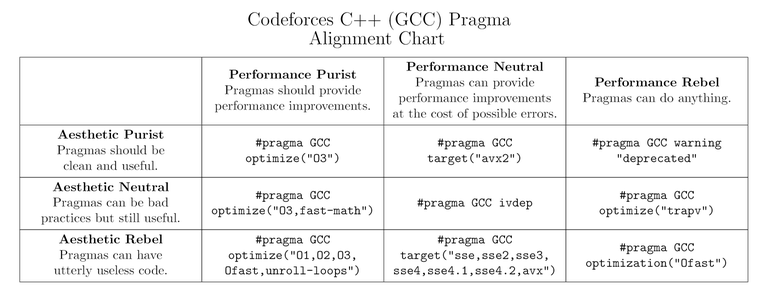
\includegraphics[width=17cm]{pragmatabel.png}% Joonise suurus, joonise fail
    \allikas{Codeforces. GCC Optimization Pragmas}% Allikas
    \label{pragmas}% Selle järgi viidatakse, pärast käsku \caption
    \end{table}
    
    Järgides ülemise tabeli nõuandeid, soovitab autor kasutada allpool kujutatud pragmade kombinatsiooni(kopeeri $main()$ funktsoonist väljapoole)\parencite{pragmas}.

\begin{cclol}
    #pragma GCC optimize("O3,unroll-loops")
    #pragma GCC target("avx2,bmi,bmi2,popcnt,lzcnt")
\end{cclol}
    \begin{kk}[H]
    \caption{Kasulikud pragmad}% Allkiri
    \allikas{Autori implementatsioon}% Allikas
    \end{kk}



        
   


    \chapter{Koordinaatide pakkimine}\label{lisa8}
    \tiny
    \normalsize
    Võte on kasulik juhul, kui hoolime ainult mingite asjade relatiivsest järjekorrast teljestikul ja arvude võimaliku väärtuse vahemik on palju suurem kui arvude arv ise, nt juhul kui antakse sisendiks koordinaadid maksimaalse väärtusega $10^9$, siis me ei hakka neid paigutama nii suurele massiivile, sest see võib hiljem põhjustada ajalimiidi ületamist(TLE), mälulimiidi ületamist(MLE), kui ka Stack Overflow'i.

    Autor soovitab neil, kes pole kindel, et nad said selgitusest aru proovida lahendada USACO Silver/Bronze division ülesannet nimega Load Balancing\parencite{load}.

\chapter{Ajakeerukus}\label{lisa9}
    \tiny
    \normalsize
Ajakeerukus on väga laialdaselt kasutus olev idee nii võistlusprogrammeerimises kui ka teoreetilises arvutiteaduses.

Võistlusprogrammeerimises on levinum notatsioon suure $O$ notatsioon, vahepeal kuigi kasutatakse ka $\Theta$ ja $\Omega$ notatsiooni.

Suure $O$ notatsioonist saab mõelda kui niinimetatud halvima juhu notatsioonist, ehk märgitakse ajakeerukust halvimal juhul, näiteks kui otsime massiivist arvu $x$, siis on võimalik, et leiame selle kohe, siis ei oleks ajakeerukus $O(1)$, vaid ikkagi $O(N)$ põhjusel, et eksisteeris ka võimalus, kus element $x$ asus massiivi teises otsas.

Suure $O$ notatsioonis ignoreeritakse ka konstante, mis tähendab, et kui vaatame kahte $O(1)$ ajakeerukusega operatsiooni, siis võib siiski nende tegelik jooksutamisaeg erineda põhjusel, et arvuti suudab teha ühte operatsiooni teha kiiremini kui teist.

Juhul, kui tuleb ülesannete lahendamisel ette, et programm on liiga aeglane, kuid olles täitse veendunud, et ajakeerukus on piisav, siis võibki põhjuseks olla suur konstant mingil operatsioonil.
\chapter{Modulaarne aritmeetika}\label{lisa10}
    \tiny
    \normalsize
Selles lisas on antud väga lühike kokkuvõte modulaararitmeetikast ja selle omadustest.

Modulaarne aritmeetika tegeleb arvude jääkidega, kus tehe kujul $x\ mod\ m$  on võrdne arvu $x$ jäägiga $m$-ga jagamisel.

Võistlusprogrammeerimises peamine modulaararitmeetika kasu tuleneb sellest, et tihti selle asemel, et teha tehteid arvudega ise saame lihtsalt teha samu tehteid nende jääkidega ilma vastust mõjutamata, näiteks võib juhtude, et mingi lõigu summa on nii suur, et ei mahu isegi unsigned long long andmetüüpi ära, kuid võttes igal liitmisel jäägi saame selle summa teha väga palju väiksemaks.

Siin on välja toodud mõned modulaarses aritmeetikas kehtivad seosed:

$$(a+b) \bmod m = (a \bmod m + b \bmod m) \bmod m$$

$$(a-b) \bmod m = (a \bmod m - b \bmod m) \bmod m$$

$$(a \cdot b) \pmod{m} = ((a \bmod m) \cdot (b \bmod m)) \bmod m$$

$$a^b \bmod {m} = (a \bmod m)^b \bmod m$$


 \chapter{Prefiksi summad}\label{lisa11}
    \tiny
    \normalsize
Prefiksi summa on võtte, mis võimaldab lõigul summa leidmist keerukusega $O(1)$, kuid massiivi ülesehitamine operatsioonide võimaldamiseks on ajakeerukusega $O(N)$ -- kus $N$ on massiivi suurus.

Naiivselt operatsioone tehes teame, et ajakeerukus oleks $O(NQ)$, kus $Q$ on päringute arv ja $N$ massiivi suurus.
Kui $N, Q \leq 10^5$, siis $NQ$ on kuni $10^{10}$, see kindlasti ei sobi.

Sellisel juhul saamegi kasutada prefiksi summat.
Selle võimaldamiseks defineerime massiivi nimega prefiks, kus märgime prefiks$[0]=0$ et vältida massiivi piiridest välja liikumist.
arr tähistab algset massiivi.

Leiame siis prefiksi summa järgnevalt:
$$
\texttt{prefix}[k]=\sum_{i=1}^{k} \texttt{arr}[i]
$$

Ehk iga k kohta teeme:
$$
\texttt{prefix}[k]=\texttt{prefix}[k-1]+\texttt{arr}[k]
$$

Saaksime teha järgnevat, et leida summa lõigul: 
$$
\sum_{i=L}^{R} \texttt{arr}[i] = \sum_{i=1}^{R} \texttt{arr}[i] - \sum_{i=1}^{L-1} \texttt{arr}[i]
$$

Kuid see on suboptimaalne, ning saame kasutada ära meie uut arvutatud massiivi: 
$$
\sum_{i=L}^{R} \texttt{arr}[i]= \texttt{prefix}[R]-\texttt{prefix}[L-1]
$$

Lihtne on täheldada, et ajakeerukus ongi selle juhul $O(N)$.

Käsitleme nüüd näidispäringut, kus $a = 2$ ja $b = 5$.
massiiviist on näha, et see oleks:
$$
\sum_{i=2}^{5} \texttt{arr}[i] = 6 + 4 + 2 + 5 = 17.
$$
\begin{figure}[H]% [] sisse märgitakse paigutus H
    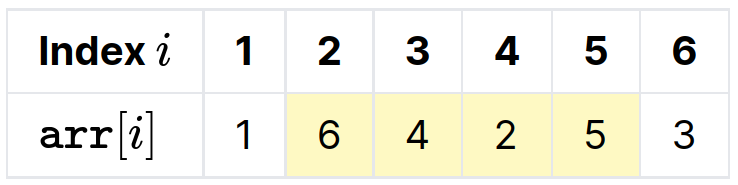
\includegraphics[width=8cm]{PrefixMassiiv1.png}% Joonise suurus, joonise fail
    \caption{Naiivselt leitud summa}% Allkiri
    \allikas{USACO Guide}% Allikas
    \label{EMaxx}% Selle järgi viidatakse, pärast käsku \caption
\end{figure}
Prefiksi summade abil saaksime teha:
$$
\texttt{prefix}[5] - \texttt{prefix}[1] = 18 - 1 = 17.
$$

\begin{figure}[H]% [] sisse märgitakse paigutus H
    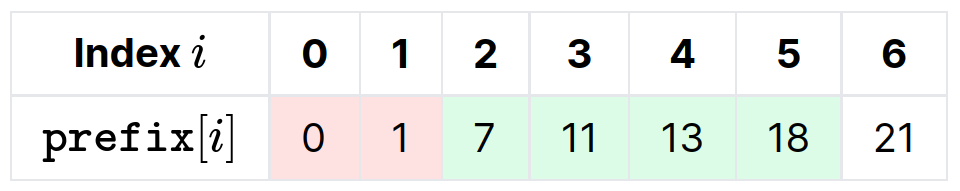
\includegraphics[width=8cm]{PrefiksMassiiv2.png}% Joonise suurus, joonise fail
    \caption{Prefiksi summa võttega leitud summa}% Allkiri
    \allikas{USACO Guide}% Allikas
    \label{EMaxx}% Selle järgi viidatakse, pärast käsku \caption
\end{figure}


\textbf{USACO ülesandeid prefiksi summade kohta}

\begin{itemize}
    \item USACO December 2015 Silver Problem 3: \href{http://usaco.org/index.php?page=viewproblem2&cpid=572}{Breed Counting} 
    \item USACO January 2016 Silver Problem 2:\href{http://usaco.org/index.php?page=viewproblem2&cpid=595}{Subsequences Summing to Sevens} 
    \item USACO December 2017 Silver Problem 1: \href{http://www.usaco.org/index.php?page=viewproblem2&cpid=762}{My Cow Ate My Homework} 
    \item USACO January 2017 Silver Problem 2: \href{http://www.usaco.org/index.php?page=viewproblem2&cpid=691}{Hoof, Paper, Scissors} 
    \item (Lisa 12) USACO February 2019 Silver Problem 2: \href{http://www.usaco.org/index.php?page=viewproblem2&cpid=919}{Painting the Barn} 
    \item Subarray Divisibility(vt peatükk 2.2.3.1.1.)
    \item Subarray Sums II(vt peatükk 2.2.3.1.2.)
    \item Multiple of 2019(vt peatükk 2.2.3.1.4.)
    \item Forest Queries(vt peatükk 2.2.3.1.3.)
    \item Cow Hopscotch(vt peatükk 2.2.3.1.5.)
\end{itemize}


    \chapter{2D prefiksi summad}\label{lisa12}
    \tiny
    \normalsize
Siin käsitleme kuidas leida $O(NQ)$, ajakeerukusega summat 2D massiivil.
Ütleme, et meil on järgnev massiiv:
  \begin{figure}[H]% [] sisse märgitakse paigutus H
    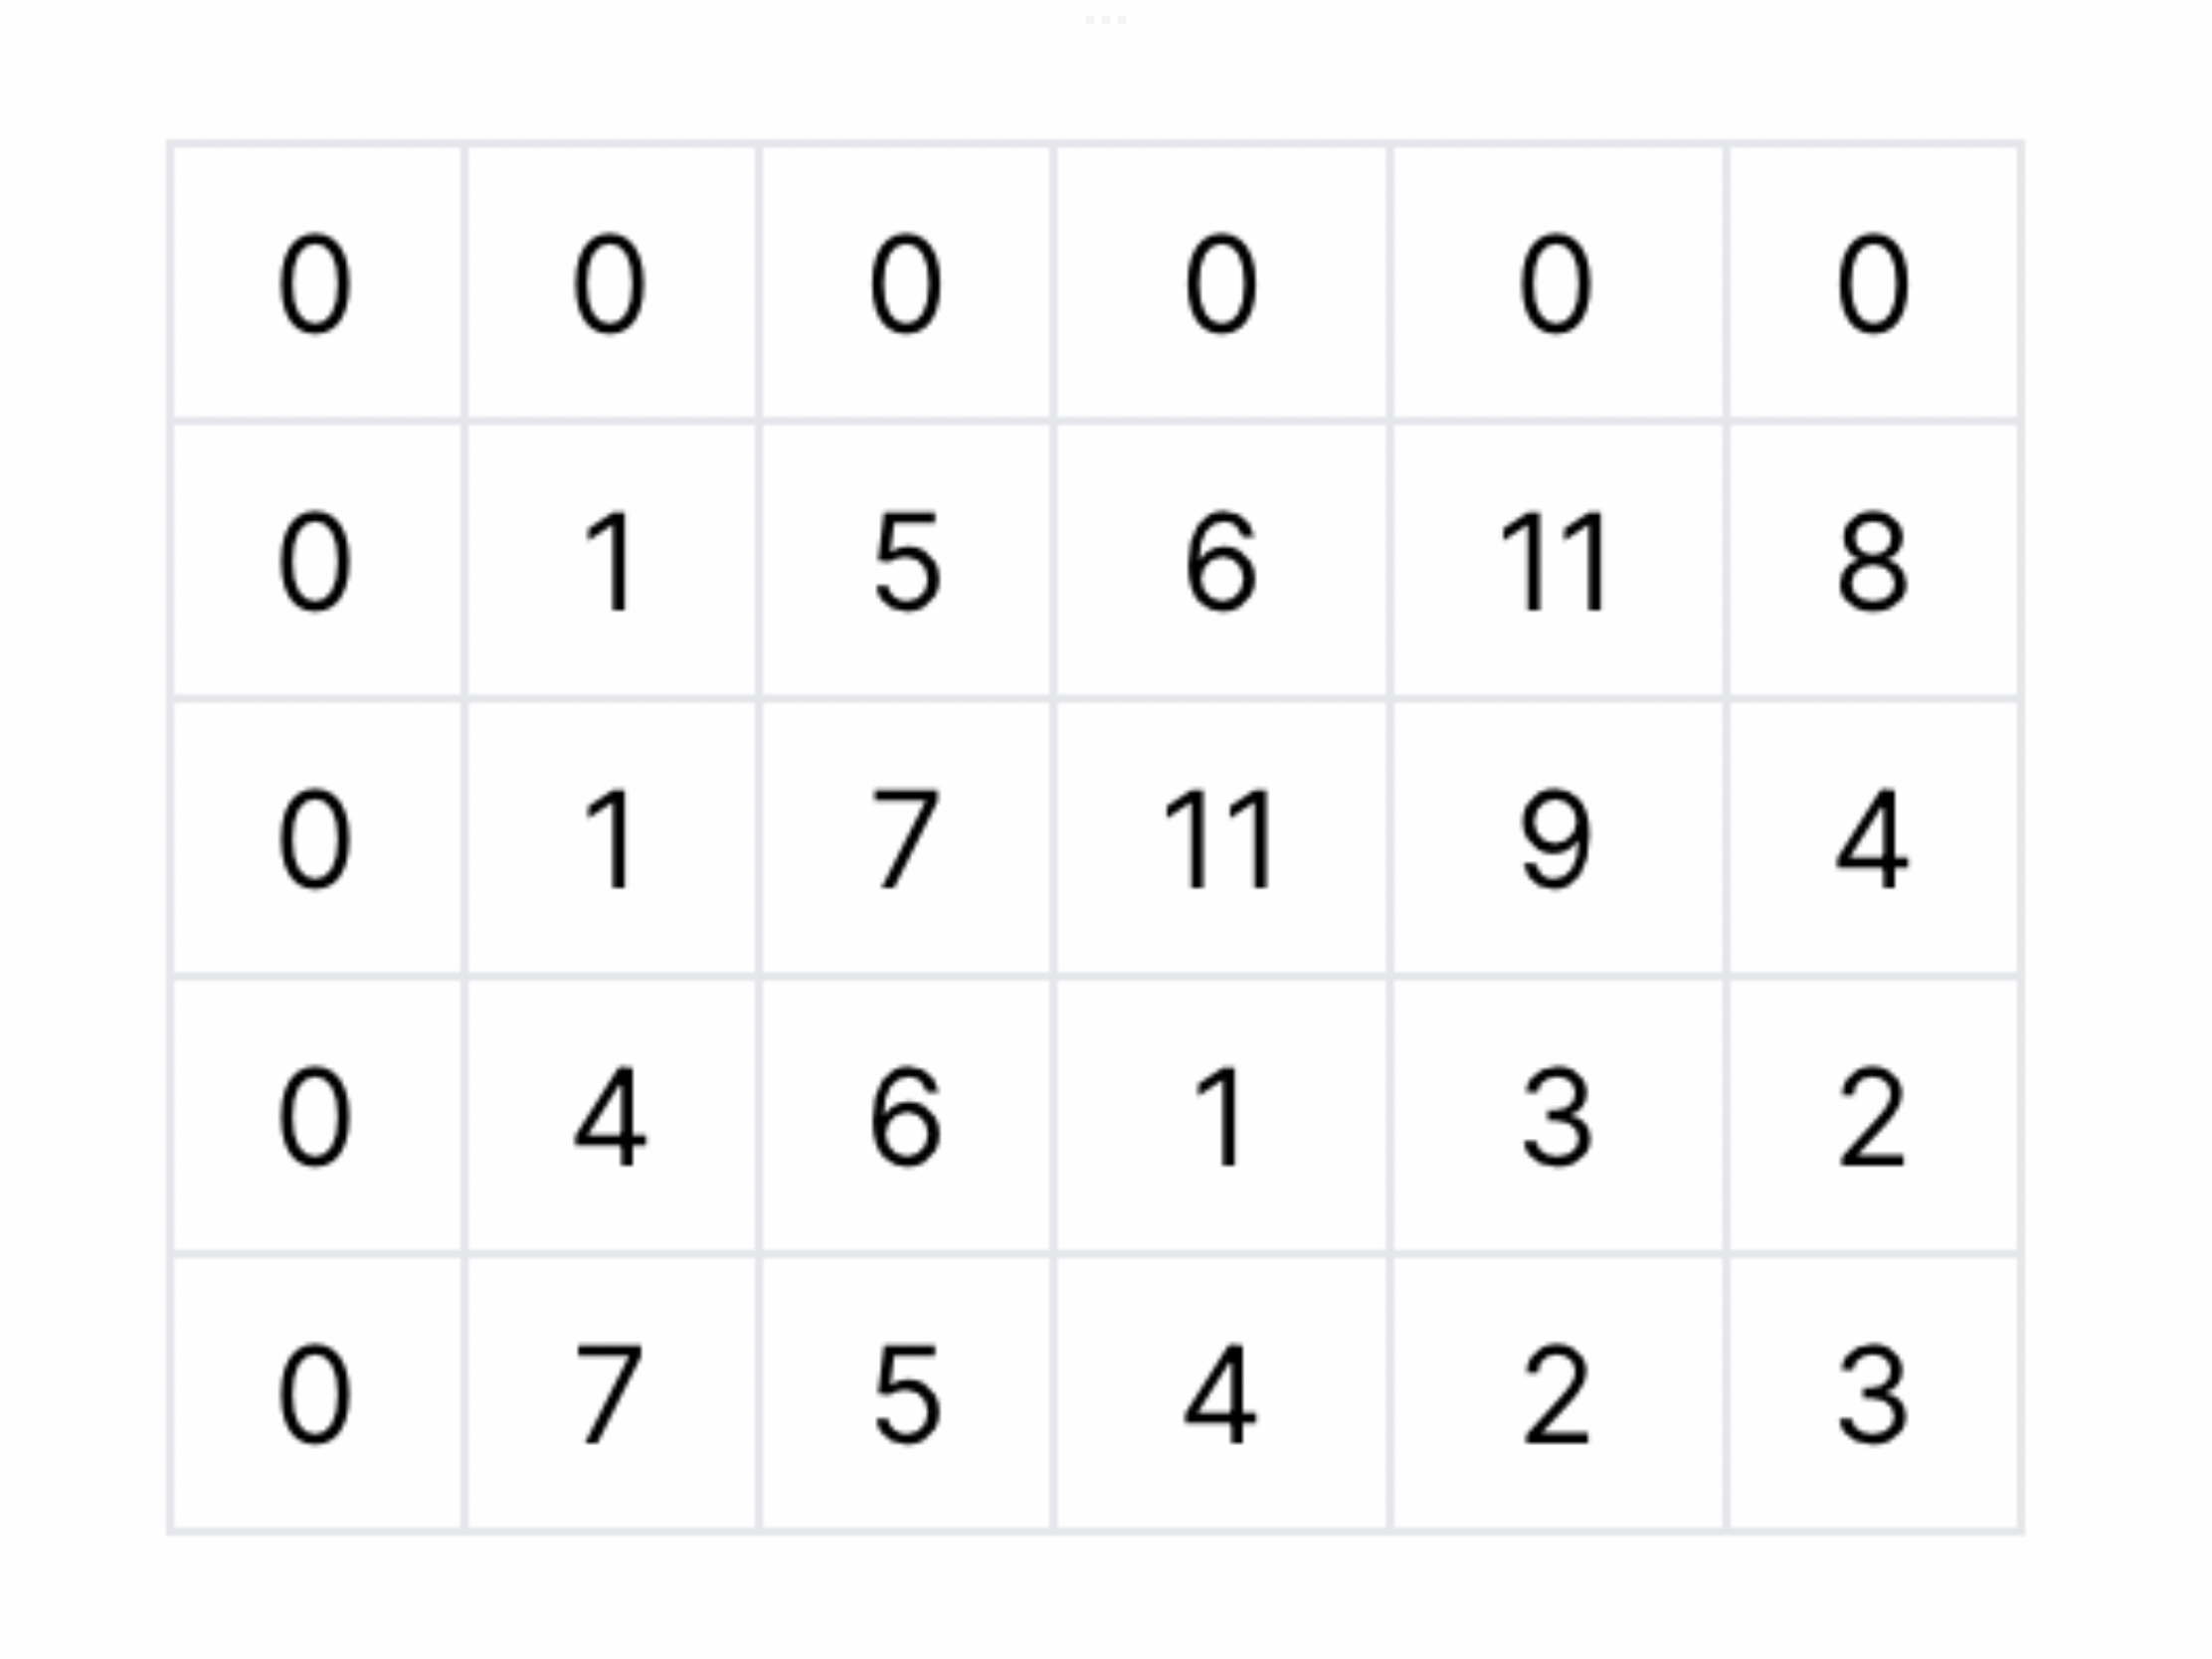
\includegraphics[width=8cm]{pr1.png}% Joonise suurus, joonise fail
    \caption{Algne massiiv}% Allkiri
    \allikas{USACO Guide}% Allikas
    \label{EMaxx}% Selle järgi viidatakse, pärast käsku \caption
\end{figure}
Kui leida summa naiivselt oleks ajakeerukuseks $O(QNM)$, kus $Q$ on päringute arv, $N$ on ridade arv, ning $M$ on veergude arv.
\begin{figure}[H]% [] sisse märgitakse paigutus H
    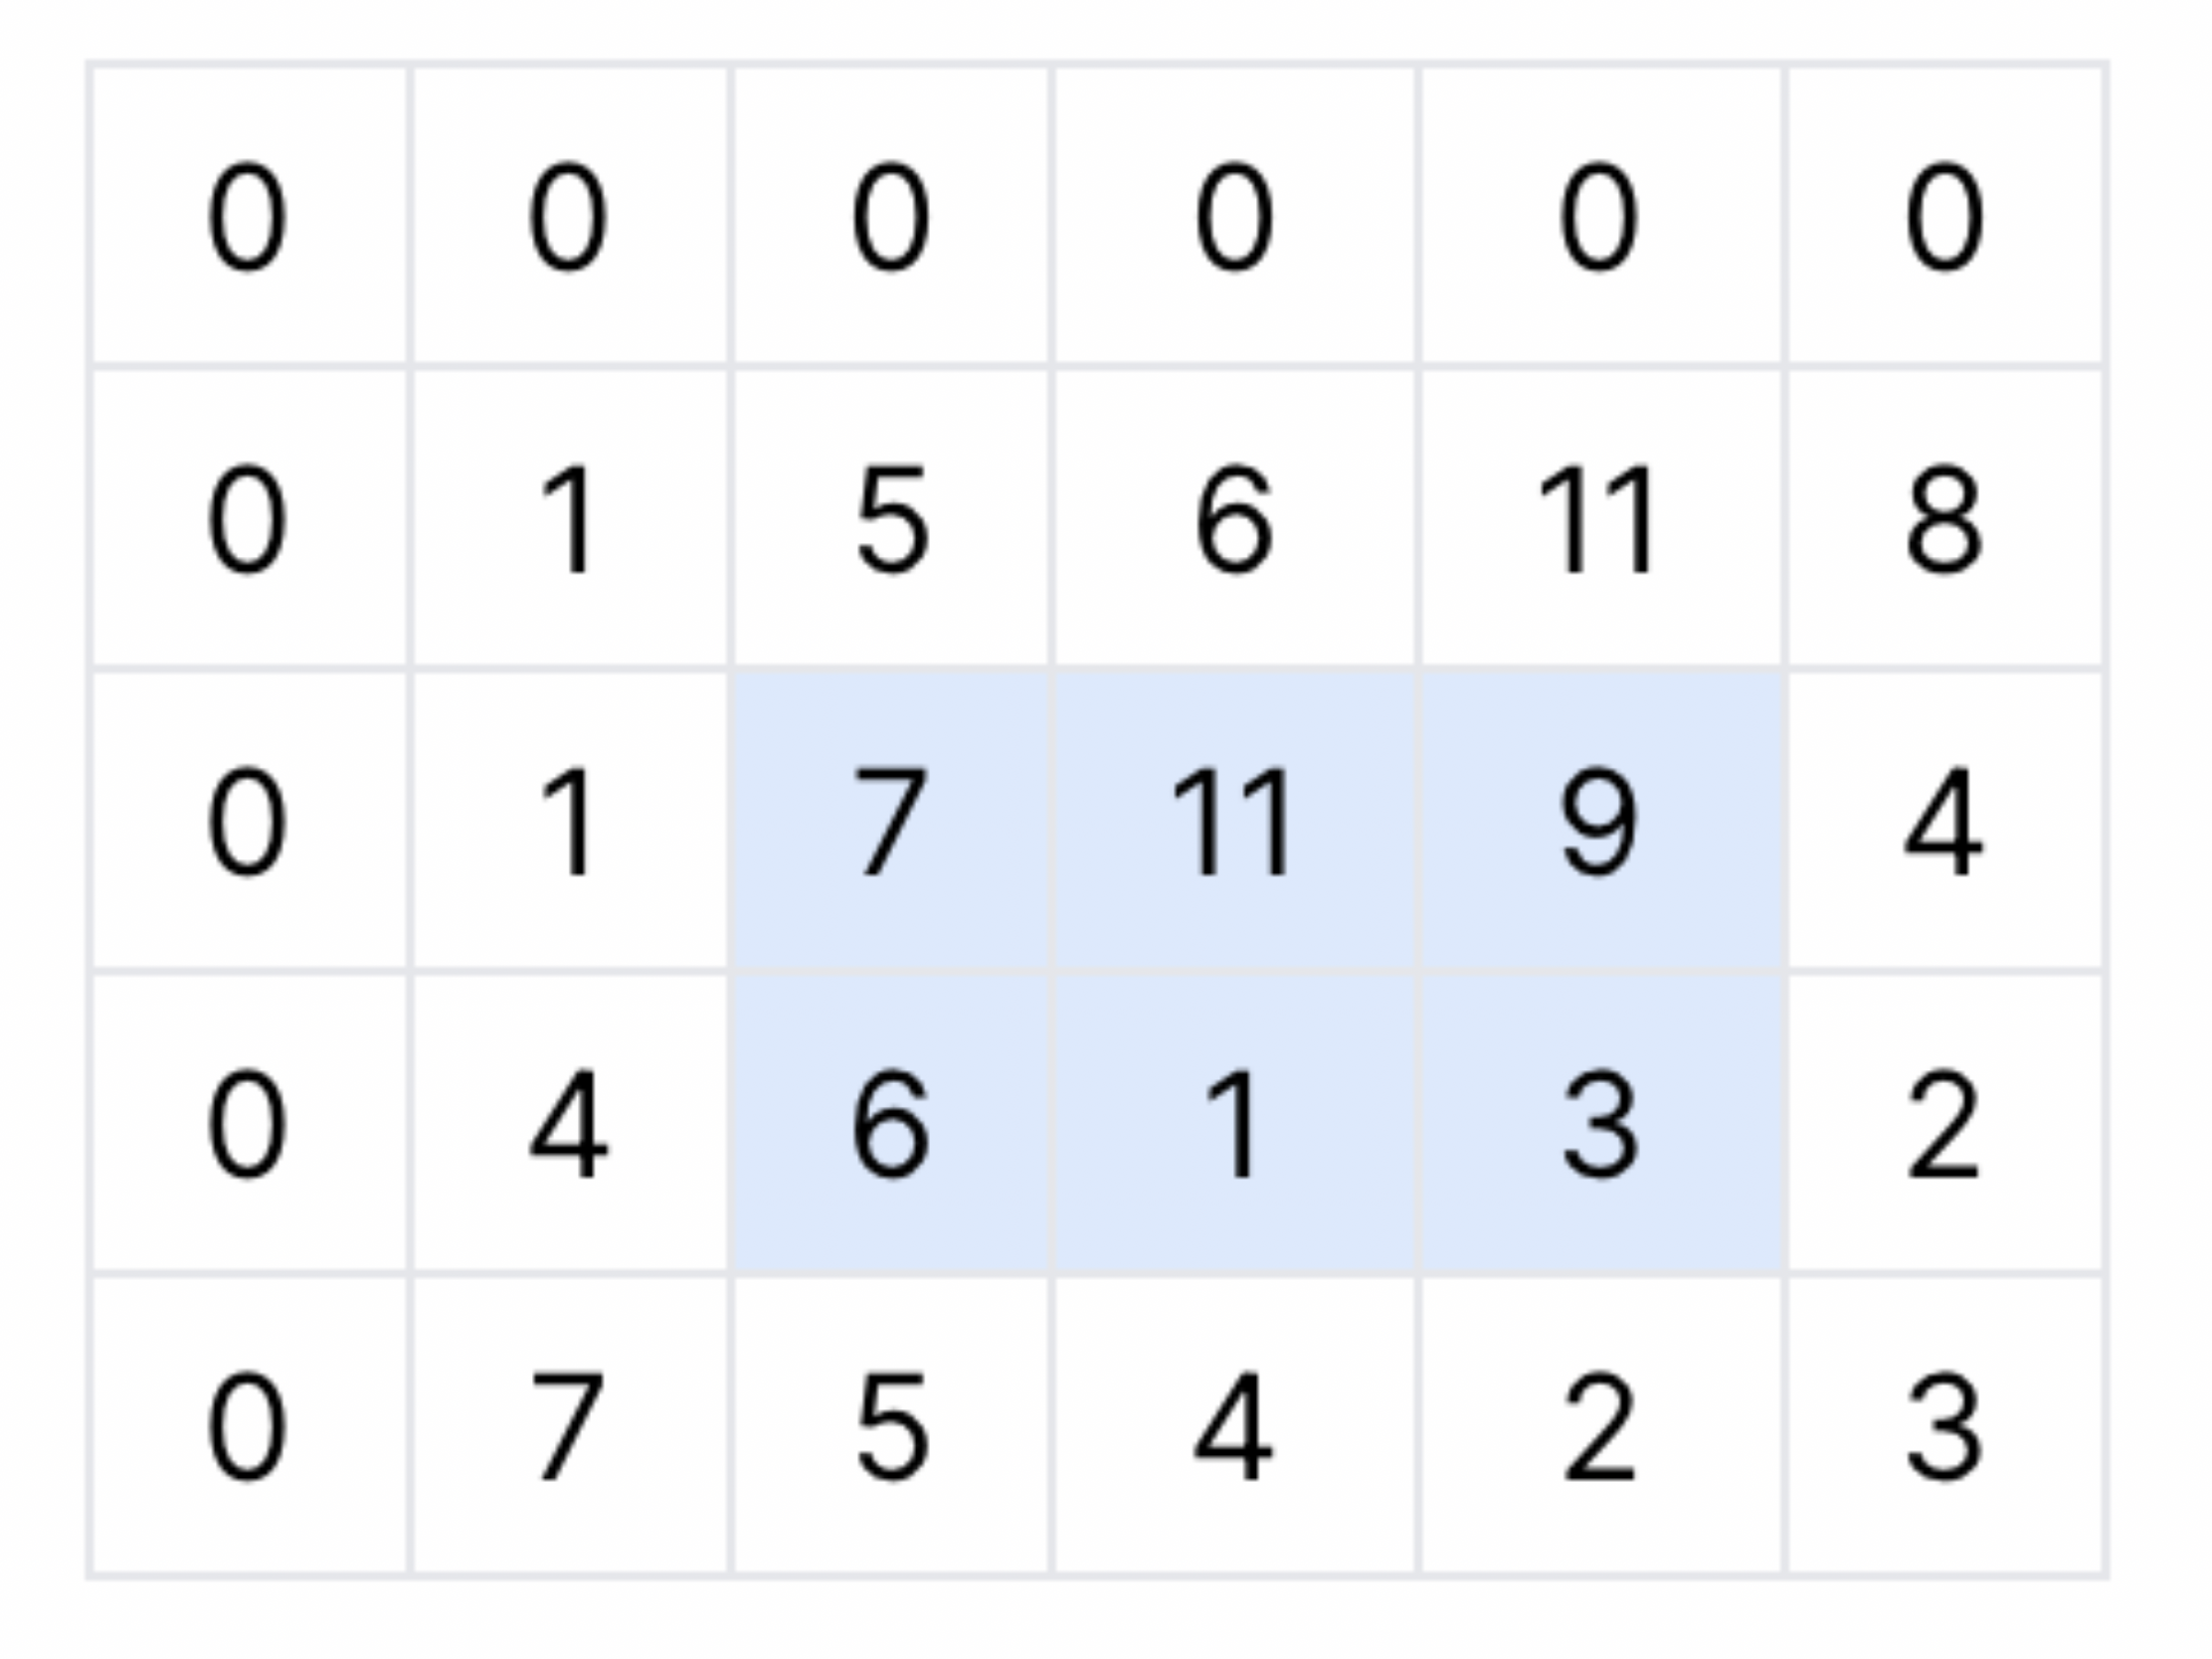
\includegraphics[width=8cm]{pr4.png}% Joonise suurus, joonise fail
    \caption{Vaadeldav alammaatriks}% Allkiri
    \allikas{USACO Guide}% Allikas
    \label{EMaxx}% Selle järgi viidatakse, pärast käsku \caption
\end{figure}

Esimene optimisatsioon mida võiks märgata, on lihtsalt leida iga $N$ rea kohta eraldi prefiksi summa, siis oleks ajakeerukuses $O(QN)$, kuid see ei ole siiski optimaalne.

\begin{figure}[H]% [] sisse märgitakse paigutus H
    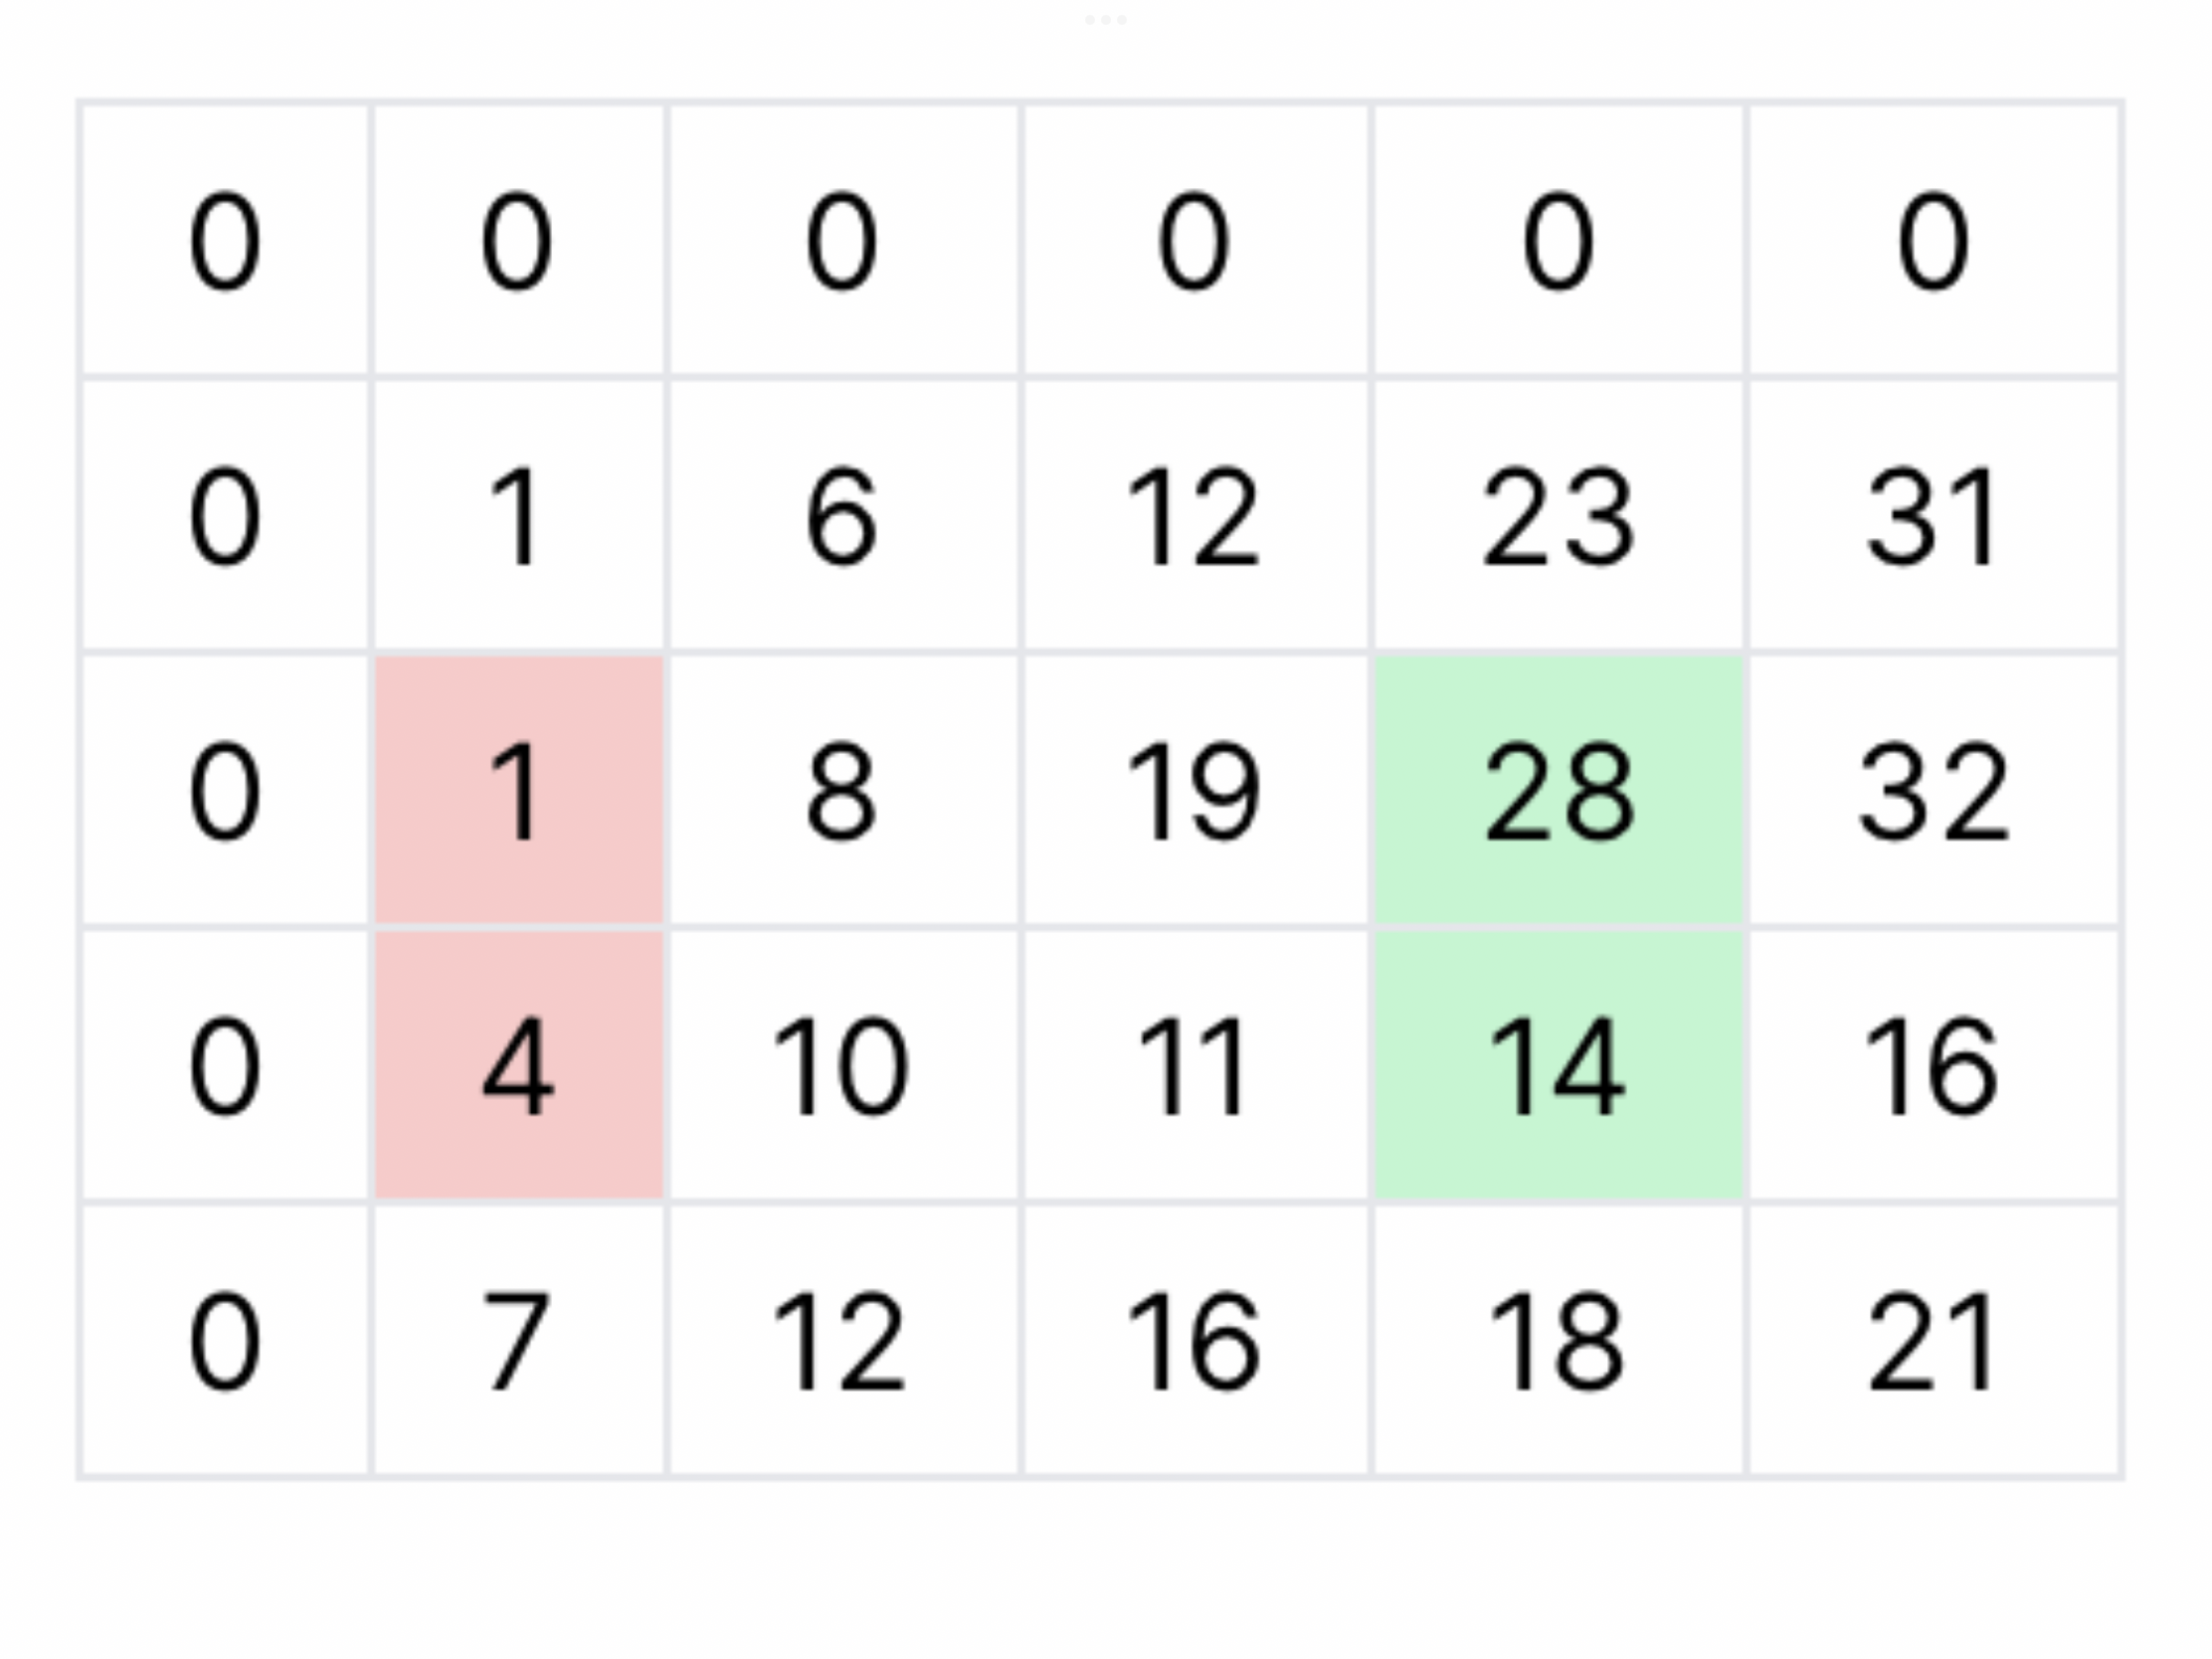
\includegraphics[width=8cm]{pr2.png}% Joonise suurus, joonise fail
    \caption{Summa leidmine kasutades 1D prefiksi summa võtet}% Allkiri
    \allikas{USACO Guide}% Allikas
    \label{EMaxx}% Selle järgi viidatakse, pärast käsku \caption
\end{figure}

Võimalik on leida 2D prefiksi summat, $O(1)$ ajakeerukusega peale $O(NM)$ eelarvutamist.


Saame võimaldada seda, kui teeme enne päringuid operatsiooni kujul:
$$
\texttt{prefix}[a][b]=\sum_{i=1}^{a} \sum_{j=1}^{b} \texttt{arr}[i][j].
$$

Ehk saame:
$$
\begin{aligned}
\texttt{prefix}[i][j] =& \, \texttt{prefix}[i-1][j]+ \texttt{prefix}[i][j-1] \\
	&- \texttt{prefix}[i-1][j-1]+ \texttt{arr}[i][j]
\end{aligned}
$$

Nüüd saame võimaldada päringuid järgneval kujul:
$$
\begin{aligned}
\sum_{i=a}^{A} \sum_{j=b}^{B} \texttt{arr}[i][j]=&\,\texttt{prefix}[A][B]
		- \texttt{prefix}[a-1][B] \\
		&- \texttt{prefix}[A][b-1] + \texttt{prefix}[a-1][b-1]
\end{aligned}
$$


Järgneval näidismassiivi summeerides rohelise ruudu väärtuse, lahutades punaste ruutude summa, ning seejärel liites halli ruudu väärtuse, saame:
$$
65-23-6+1 = 37,
$$
\begin{figure}[H]% [] sisse märgitakse paigutus H
    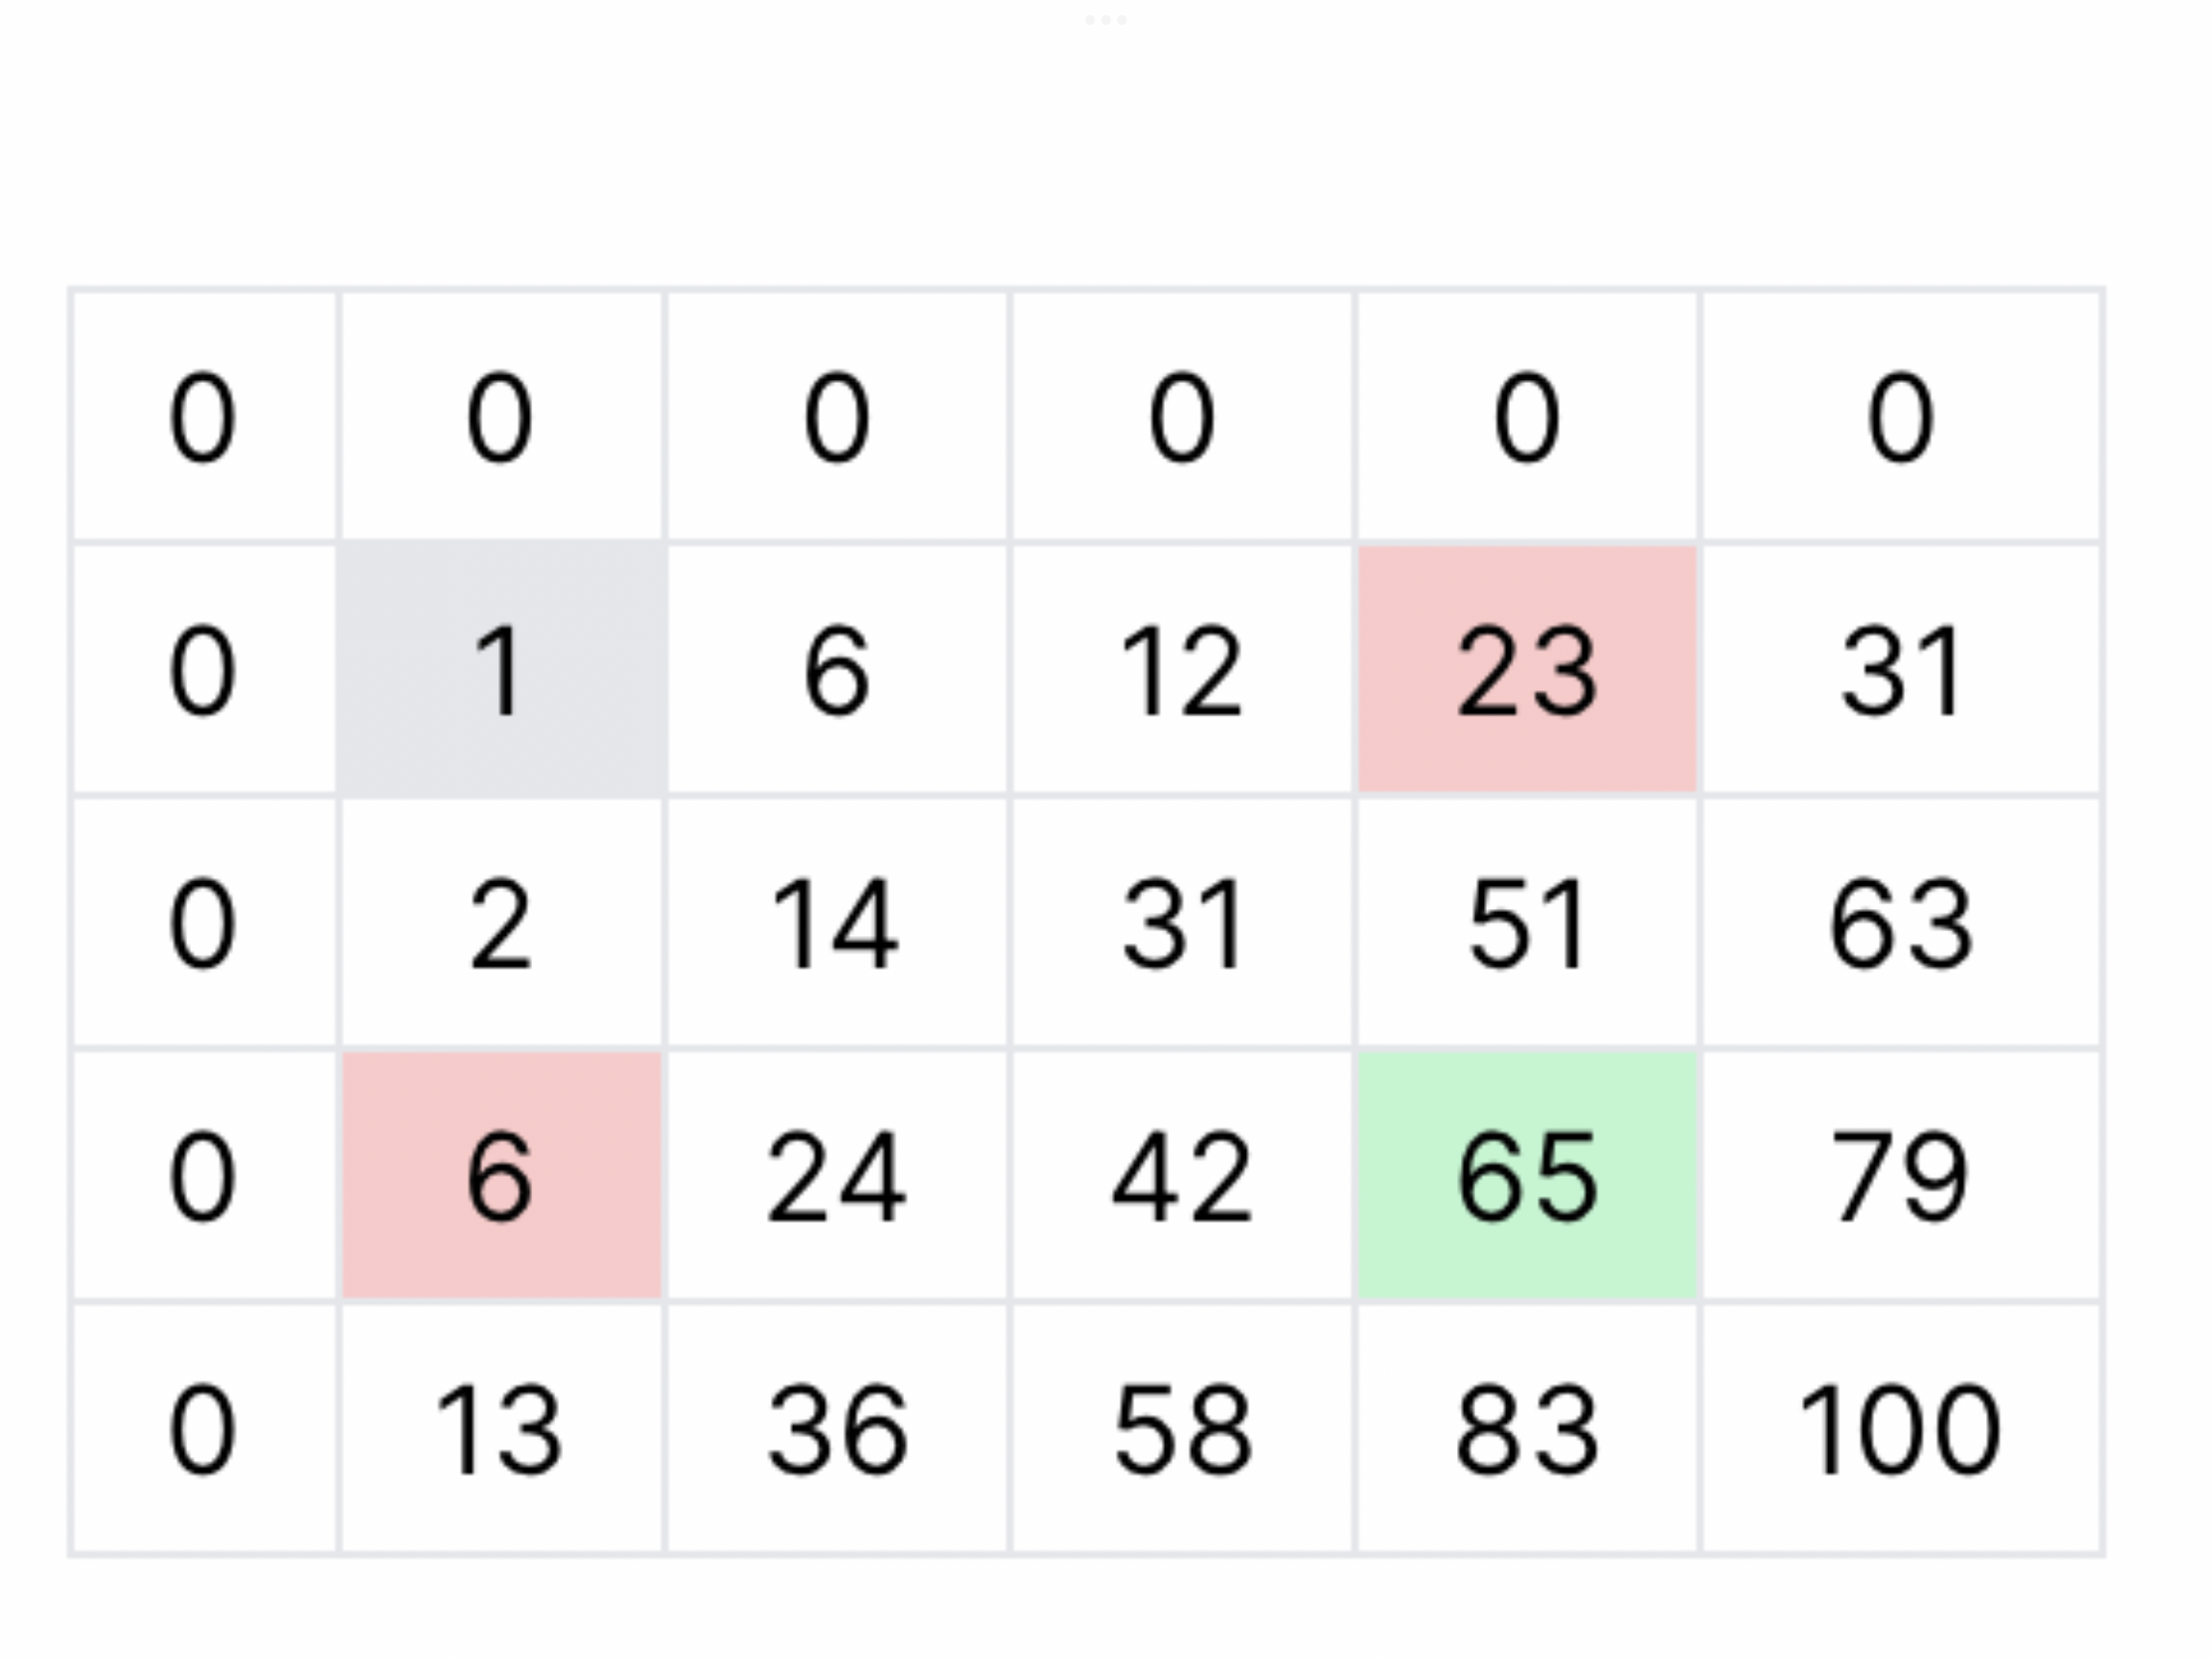
\includegraphics[width=8cm]{pr3.png}% Joonise suurus, joonise fail
    \caption{Summa leidmine effektiivselt 2D prefiksi summa võtte abil}% Allkiri
    \allikas{USACO Guide}% Allikas
    \label{EMaxx}% Selle järgi viidatakse, pärast käsku \caption
\end{figure}

 \chapter{Indekseeritud hulk ehk order statistic tree andmestruktuur}\label{lisa13}
    \tiny
    \normalsize
Indexed set on policy-based andmestruktuur mis ei ole C++ standardi osa, kuid on GNU kompilaatoriga kaasas(kusjuures GNU on kasutusel ka Eesti Informaatikaolümpiaadil).

Andmestruktuuri eelis seisneb selles, et see saab täita mõningaid lõikude puu ülesandeid sama hea ajakeerukusega, kuid vähesema koodiga.
Näiteks saab lahendada võistlusprogrammeerimises inversioonide arvu leidmise ja $k$-nda elemendi otsimise ülesannet sobiliku kiirusega.

Indexed set andmestruktuuri operatsioonidele on üldjuhul omane ajakeerukus $O(\log N)$.

Andmestruktuur on omadustelt sarnane std::set konteinerile, ehk konteineri elemendi on sorteeritud suurenevas järjekorras, ning duplikaadid ei ole lubatud.
Eelis std::set ees seisneb kahes lisa funktsionaalsuses:
\begin{enumerate}
    \item order\_of\_key(x) -- funktsioon leiab elemendi $x$ asukoha massiivis, juhul kui elementi ei ole massiivis siis tagastatakse elemendi asukoht juhul kui ta oleks massiivis. 
    \item find\_by\_order(x) -- funktsioon leiab mis element on asukohal $x$(loendamine algab nullist), tagastatakse viide elemendile.
\end{enumerate}

Andmestruktuuri peamine miinus tuleneb selle suurest mälukasutusest(nn masinapool on kasutusel tasakaalustatud puu, mis ehitab üleliigseid tippe).

Järgnev koodilõik näitab kuidas importida andmestruktuuri ja kasutada seda koodis:

\begin{cclol}
    #include <bits/stdc++.h>
    using namespace std;

    // Importimine ja vormi spetsifitseerimine
    #include <ext/pb_ds/assoc_container.hpp>
    using namespace __gnu_pbds;
    
    typedef tree<int, null_type, less<int>, rb_tree_tag, 
    order_statistic_tree_node_update> inset;
//Kusjuures typedef juures saad ka määrata ära näiteks missuguseid 
//andmeid inset kasutab(nt saad asendada int-i, pair<int, int>-ga), 
//veel saab muuta sorteerimist 
//asendades less<int>, greater<int> vastu.

    int main(){
    inset hulk; // see on meie indexed set
    hulk.insert(1); hulk.insert(3); hulk.insert(2);
    cout << order_of_key(3); // saame vastuseks 2
    cout << *find_by_order(0); // saame vastuseks 1
    
    return 0;
    }
    \end{cclol}
    \begin{kk}[H]
    \caption{Order statistic tree}% Allkiri
    \allikas{Autori implementatsioon}% Allikas
    \end{kk}


    Tihti on vaja ülesannetes kasutada mitmeid sama väärtudega elemente, sel juhul on parim variant kasutada std::pair kus teine element on nt elemendi sisendisse võtmise indeks for-loopis.

\textbf{Ülesanded}
\begin{itemize}
\item Mega Inversions(vt peatükk 2.2.3.2.4.)
\item Why did the Cow Cross the Road III(vt peatükk 2.2.3.2.5.)
\item List Removals(vt peatükk 2.2.3.2.1.)
\item Salary Queries(vt peatükk 2.2.3.2.3.)
\item Inversions(vt peatükk 2.2.3.2.2.)
\item Balanced Photo(vt peatükk 2.2.3.2.6.)
\item Haircut(vt peatükk 2.2.3.2.7.)
\item Sleepy Cow Sorting(vt peatükk 2.2.3.2.8.)
\end{itemize}
 \chapter{Testide genereerimine}\label{lisa14}
    \tiny
    \normalsize

    Testide genereerimiseks kõige lihtsam viis(kui neid väga palju ei taha teha), on teha programm, mis väljastab suvalisi arve ülesande tekstis märgitud vahemikus.

    Selle jaoks saab kasutada alumist koodilõiku:
    \begin{cclol}
    int b = 1000000; // maksimaalne väärtus
    int c = 1;      // minimaalne väärtus
    int a = rand() % b + c; cout << a;
    \end{cclol}
    \begin{kk}[H]
    \caption{rand() funktsiooni kasutamine}% Allkiri
    \allikas{Autori implementatsioon}% Allikas
    \end{kk}

\chapter{Eesti Informaatikaolümpiaad 2022/23 II valikvõistlus, ülesanne "Kaardid"}\label{lisa15}
    \tiny
    \normalsize
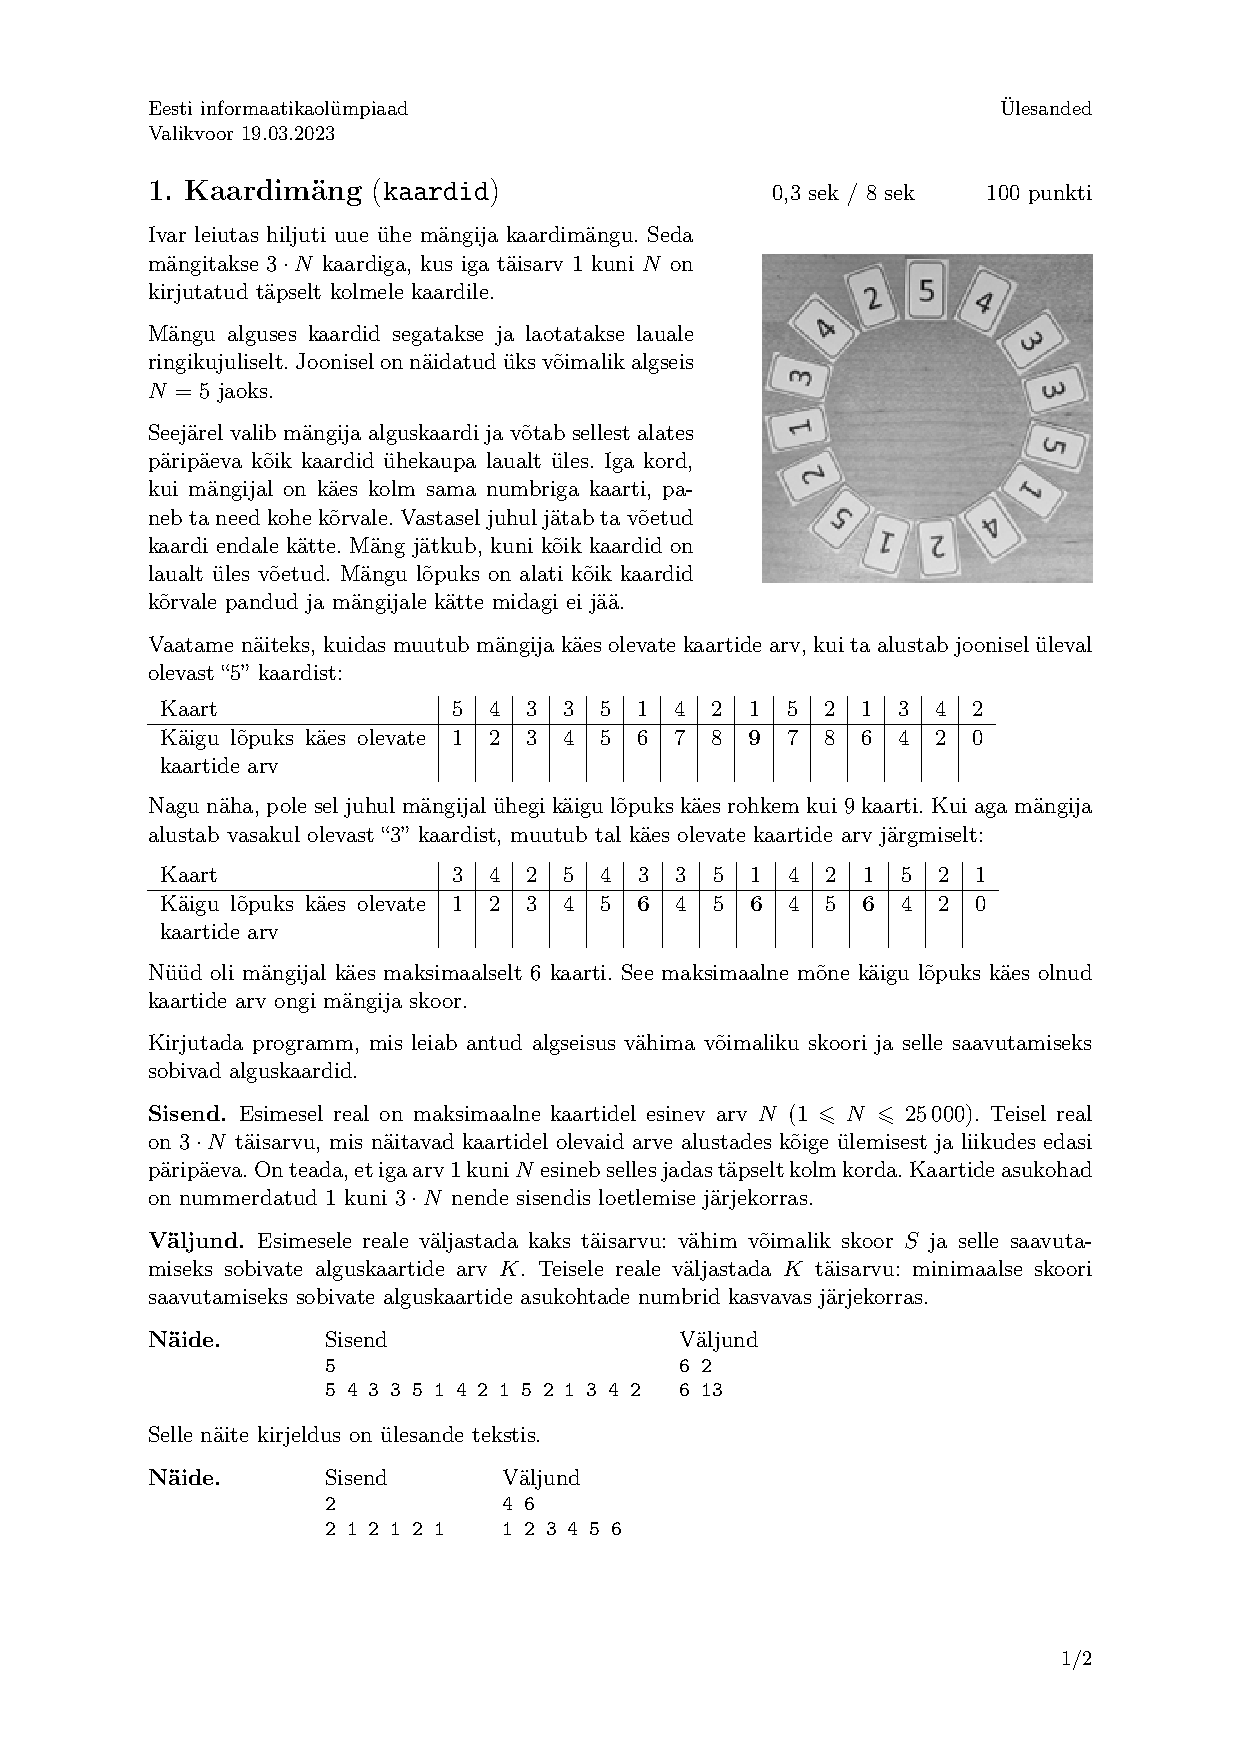
\includepdf[pages=-]{kaardid (et).pdf}
\end{appendices}


\addchap{Resümee}

Lõikude puule leidub väga palju väljundeid võistlusprogrammeerimises, ning juhul kui lugeja on piisavalt kaugel oma tasemega, on tegu vajaliku teadmisega, et saavutada häid tulemusi olümpiaadidel. Kuigi töös on kõigile ülesannetele toodud ka välja lahendus ja implementatsioon, soovitab autor siiski proovida ülesandeid ise lahendada, enne muidugi tutvudes vajaliku teooriaga.

Uurimistöö eesmärgiks oli koostada põhjalik eestikeelne materjal lõikude puu kohta võistlusprogrammeerimises. Tegu on hea lisamaterjaliga lõikude puuga tutvumiseks, olles kas lihtsalt huvitatud teemast või harjutamas Eesti Informaatikaolümpiaadi jaoks. Eriti kasulik on materjal neile kelle inglise keele tase pole piisavalt hea, et kasutada teisi materjale, sellel juhul on tegu ainsa nii põhjaliku allikaga teemal.

\addchap{Abstract}

\textbf{Segment tree in competitive programming}

Segment trees have numerous practical applications in competitive programming. Acquiring knowledge of segment trees is crucial for achieving good results in Olympiad competitions. Although the solutions and implementations of all tasks are readily available in the work, the author encourages readers to attempt solving the tasks themselves, after becoming familiar with the necessary theory.

The purpose of this paper is to provide a comprehensive resource in Estonian for understanding the uses of segment trees in competitive programming. It serves as a valuable additional resource for those interested in the topic or preparing for the Estonian Informatics Olympiad. This material is especially useful for individuals with limited proficiency in English, as it is the only comprehensive source available on the subject in Estonian.

\kinnitusleht


\end{document}
